% ------------------ DOCUMENT SETUP ------------------ 
\documentclass{report} % Document class and options
% ------------------ PACKAGES ------------------ 

% Packages add extra commands and features to your LaTeX document. 
% Here are some of the most common packages for a thesis document.

% Floating environments for figures and tables
\usepackage{float}

% Color support
\usepackage{color}

% Epigraphs
\usepackage{epigraph}

% Color support for tables
\usepackage[table,xcdraw]{xcolor}

% Mathematical typesetting
\usepackage{amsthm}

% Theorem environments
\newtheorem{corollary}{Corollary}[section]
\newtheorem{definition}{Definition}[section]
\newtheorem{theorem}{Theorem}[section]
\newtheorem{lemma}{Lemma}[section]
\newtheorem{proposition}{Proposition}[section]
\newtheorem{example}{Example}[section]

% Remark environment
\theoremstyle{remark}
\newtheorem{remark}{Remark}

% Restatable theorems
\usepackage{thmtools}
\usepackage{thm-restate}
\declaretheorem[name=Proposition,numberwithin=section]{proprep}
\newtheorem{thm}{Theorem}

% Algorithms
\usepackage[ruled,vlined]{algorithm2e}
\usepackage{algorithmic}

% Vector arrows
\usepackage{esvect}

% TikZ for diagrams
\usepackage{tikz}
\usetikzlibrary{patterns, bayesnet, arrows, backgrounds}

% Hyperlinks
\usepackage{hyperref}
\hypersetup{
    citecolor = blue
}

% Multi-row tables
\usepackage{multirow}

% Appendices
\usepackage[toc,page]{appendix}

% Captioning figures and tables
\usepackage[format=hang,font=normalsize,labelfont=bf,labelsep=colon,singlelinecheck=off, justification=centering]{caption}
\usepackage{subcaption}

% Long tables
\usepackage{longtable}

% Glossaries and acronyms
\usepackage[acronym]{glossaries}

% Font settings
\usepackage[scaled]{helvet}
\usepackage[T1]{fontenc}
\renewcommand\familydefault{\sfdefault}

% Input encoding
\usepackage[utf8]{inputenc}

% Empty pages
\usepackage{emptypage}

% Importing files
\usepackage{import}

% Table of Contents customization
\usepackage{tocloft}

% Title customization
\usepackage{titlesec}

% Table of Contents title customization
\usepackage{titletoc}

% Alternative implementations for LaTeX commands
\usepackage{etoolbox}

% Header and footer control
\usepackage{fancyhdr} 

% Typography enhancements
\usepackage{microtype}

% PDF bookmarks
\usepackage{bookmark}

% Units and symbols
\usepackage{gensymb}
\usepackage{textcomp}

% Bibliography
\usepackage[natbib,style=authoryear,natbib=true]{biblatex}
\addbibresource{publications.bib} % Add the .bib file that contains the references
\addbibresource{References.bib} % Add the .bib file that contains the references

% Sample text
\usepackage{blindtext}

% Tables
\usepackage{booktabs}

% Code listings
\usepackage{listings}
\usepackage{minted}

% Math symbols
\usepackage{amsmath,amsfonts,bm}
\usepackage{amssymb}

% Clever referencing
\usepackage[capitalize,noabbrev]{cleveref}

% Graphics
\usepackage{graphicx}
\usepackage{svg}

% Restating theorems
\usepackage{thm-restate}

% Line spacing control
\usepackage{setspace}

% Mini table of contents
\usepackage{minitoc} 

% Mini TOC font settings
\renewcommand{\mtifont}{\large\sffamily}
\renewcommand{\mtcfont}{\small\sffamily}
\renewcommand{\mtcSfont}{\small\sffamily}
\renewcommand{\mtcSSfont}{\small\sffamily}
\renewcommand{\mtcSSSfont}{\small\sffamily}

% Add to table of contents
\newcommand\addtotoc[1]{
  \refstepcounter{dummy}
  \addcontentsline{toc}{chapter}{#1}
}
 % Include packages
%%%%% NEW MATH DEFINITIONS %%%%%

\usepackage{amsmath,amsfonts,bm}

% Mark sections of captions for referring to divisions of figures
\newcommand{\figleft}{{\em (Left)}}
\newcommand{\figcenter}{{\em (Center)}}
\newcommand{\figright}{{\em (Right)}}
\newcommand{\figtop}{{\em (Top)}}
\newcommand{\figbottom}{{\em (Bottom)}}
\newcommand{\captiona}{{\em (a)}}
\newcommand{\captionb}{{\em (b)}}
\newcommand{\captionc}{{\em (c)}}
\newcommand{\captiond}{{\em (d)}}

% Highlight a newly defined term
\newcommand{\newterm}[1]{{\bf #1}}


% Figure reference, lower-case.
\def\figref#1{figure~\ref{#1}}
% Figure reference, capital. For start of sentence
\def\Figref#1{Figure~\ref{#1}}
\def\twofigref#1#2{figures \ref{#1} and \ref{#2}}
\def\quadfigref#1#2#3#4{figures \ref{#1}, \ref{#2}, \ref{#3} and \ref{#4}}
% Section reference, lower-case.
\def\secref#1{section~\ref{#1}}
% Section reference, capital.
\def\Secref#1{Section~\ref{#1}}
% Reference to two sections.
\def\twosecrefs#1#2{sections \ref{#1} and \ref{#2}}
% Reference to three sections.
\def\secrefs#1#2#3{sections \ref{#1}, \ref{#2} and \ref{#3}}
% Reference to an equation, lower-case.
\def\eqref#1{equation~\ref{#1}}
% Reference to an equation, upper case
\def\Eqref#1{Equation~\ref{#1}}
% A raw reference to an equation---avoid using if possible
\def\plaineqref#1{\ref{#1}}
% Reference to a chapter, lower-case.
\def\chapref#1{chapter~\ref{#1}}
% Reference to an equation, upper case.
\def\Chapref#1{Chapter~\ref{#1}}
% Reference to a range of chapters
\def\rangechapref#1#2{chapters\ref{#1}--\ref{#2}}
% Reference to an algorithm, lower-case.
\def\algref#1{algorithm~\ref{#1}}
% Reference to an algorithm, upper case.
\def\Algref#1{Algorithm~\ref{#1}}
\def\twoalgref#1#2{algorithms \ref{#1} and \ref{#2}}
\def\Twoalgref#1#2{Algorithms \ref{#1} and \ref{#2}}
% Reference to a part, lower case
\def\partref#1{part~\ref{#1}}
% Reference to a part, upper case
\def\Partref#1{Part~\ref{#1}}
\def\twopartref#1#2{parts \ref{#1} and \ref{#2}}

\def\ceil#1{\lceil #1 \rceil}
\def\floor#1{\lfloor #1 \rfloor}
\def\1{\bm{1}}
\newcommand{\train}{\mathcal{D}}
\newcommand{\valid}{\mathcal{D_{\mathrm{valid}}}}
\newcommand{\test}{\mathcal{D_{\mathrm{test}}}}

\def\eps{{\epsilon}}


% Random variables
\def\reta{{\textnormal{$\eta$}}}
\def\ra{{\textnormal{a}}}
\def\rb{{\textnormal{b}}}
\def\rc{{\textnormal{c}}}
\def\rd{{\textnormal{d}}}
\def\re{{\textnormal{e}}}
\def\rf{{\textnormal{f}}}
\def\rg{{\textnormal{g}}}
\def\rh{{\textnormal{h}}}
\def\ri{{\textnormal{i}}}
\def\rj{{\textnormal{j}}}
\def\rk{{\textnormal{k}}}
\def\rl{{\textnormal{l}}}
% rm is already a command, just don't name any random variables m
\def\rn{{\textnormal{n}}}
\def\ro{{\textnormal{o}}}
\def\rp{{\textnormal{p}}}
\def\rq{{\textnormal{q}}}
\def\rr{{\textnormal{r}}}
\def\rs{{\textnormal{s}}}
\def\rt{{\textnormal{t}}}
\def\ru{{\textnormal{u}}}
\def\rv{{\textnormal{v}}}
\def\rw{{\textnormal{w}}}
\def\rx{{\textnormal{x}}}
\def\ry{{\textnormal{y}}}
\def\rz{{\textnormal{z}}}

% Random vectors
\def\rvepsilon{{\mathbf{\epsilon}}}
\def\rvtheta{{\mathbf{\theta}}}
\def\rva{{\mathbf{a}}}
\def\rvb{{\mathbf{b}}}
\def\rvc{{\mathbf{c}}}
\def\rvd{{\mathbf{d}}}
\def\rve{{\mathbf{e}}}
\def\rvf{{\mathbf{f}}}
\def\rvg{{\mathbf{g}}}
\def\rvh{{\mathbf{h}}}
\def\rvu{{\mathbf{i}}}
\def\rvj{{\mathbf{j}}}
\def\rvk{{\mathbf{k}}}
\def\rvl{{\mathbf{l}}}
\def\rvm{{\mathbf{m}}}
\def\rvn{{\mathbf{n}}}
\def\rvo{{\mathbf{o}}}
\def\rvp{{\mathbf{p}}}
\def\rvq{{\mathbf{q}}}
\def\rvr{{\mathbf{r}}}
\def\rvs{{\mathbf{s}}}
\def\rvt{{\mathbf{t}}}
\def\rvu{{\mathbf{u}}}
\def\rvv{{\mathbf{v}}}
\def\rvw{{\mathbf{w}}}
\def\rvx{{\mathbf{x}}}
\def\rvy{{\mathbf{y}}}
\def\rvz{{\mathbf{z}}}

% Elements of random vectors
\def\erva{{\textnormal{a}}}
\def\ervb{{\textnormal{b}}}
\def\ervc{{\textnormal{c}}}
\def\ervd{{\textnormal{d}}}
\def\erve{{\textnormal{e}}}
\def\ervf{{\textnormal{f}}}
\def\ervg{{\textnormal{g}}}
\def\ervh{{\textnormal{h}}}
\def\ervi{{\textnormal{i}}}
\def\ervj{{\textnormal{j}}}
\def\ervk{{\textnormal{k}}}
\def\ervl{{\textnormal{l}}}
\def\ervm{{\textnormal{m}}}
\def\ervn{{\textnormal{n}}}
\def\ervo{{\textnormal{o}}}
\def\ervp{{\textnormal{p}}}
\def\ervq{{\textnormal{q}}}
\def\ervr{{\textnormal{r}}}
\def\ervs{{\textnormal{s}}}
\def\ervt{{\textnormal{t}}}
\def\ervu{{\textnormal{u}}}
\def\ervv{{\textnormal{v}}}
\def\ervw{{\textnormal{w}}}
\def\ervx{{\textnormal{x}}}
\def\ervy{{\textnormal{y}}}
\def\ervz{{\textnormal{z}}}

% Random matrices
\def\rmA{{\mathbf{A}}}
\def\rmB{{\mathbf{B}}}
\def\rmC{{\mathbf{C}}}
\def\rmD{{\mathbf{D}}}
\def\rmE{{\mathbf{E}}}
\def\rmF{{\mathbf{F}}}
\def\rmG{{\mathbf{G}}}
\def\rmH{{\mathbf{H}}}
\def\rmI{{\mathbf{I}}}
\def\rmJ{{\mathbf{J}}}
\def\rmK{{\mathbf{K}}}
\def\rmL{{\mathbf{L}}}
\def\rmM{{\mathbf{M}}}
\def\rmN{{\mathbf{N}}}
\def\rmO{{\mathbf{O}}}
\def\rmP{{\mathbf{P}}}
\def\rmQ{{\mathbf{Q}}}
\def\rmR{{\mathbf{R}}}
\def\rmS{{\mathbf{S}}}
\def\rmT{{\mathbf{T}}}
\def\rmU{{\mathbf{U}}}
\def\rmV{{\mathbf{V}}}
\def\rmW{{\mathbf{W}}}
\def\rmX{{\mathbf{X}}}
\def\rmY{{\mathbf{Y}}}
\def\rmZ{{\mathbf{Z}}}

% Elements of random matrices
\def\ermA{{\textnormal{A}}}
\def\ermB{{\textnormal{B}}}
\def\ermC{{\textnormal{C}}}
\def\ermD{{\textnormal{D}}}
\def\ermE{{\textnormal{E}}}
\def\ermF{{\textnormal{F}}}
\def\ermG{{\textnormal{G}}}
\def\ermH{{\textnormal{H}}}
\def\ermI{{\textnormal{I}}}
\def\ermJ{{\textnormal{J}}}
\def\ermK{{\textnormal{K}}}
\def\ermL{{\textnormal{L}}}
\def\ermM{{\textnormal{M}}}
\def\ermN{{\textnormal{N}}}
\def\ermO{{\textnormal{O}}}
\def\ermP{{\textnormal{P}}}
\def\ermQ{{\textnormal{Q}}}
\def\ermR{{\textnormal{R}}}
\def\ermS{{\textnormal{S}}}
\def\ermT{{\textnormal{T}}}
\def\ermU{{\textnormal{U}}}
\def\ermV{{\textnormal{V}}}
\def\ermW{{\textnormal{W}}}
\def\ermX{{\textnormal{X}}}
\def\ermY{{\textnormal{Y}}}
\def\ermZ{{\textnormal{Z}}}

% Vectors
\def\vzero{{\bm{0}}}
\def\vone{{\bm{1}}}
\def\vmu{{\bm{\mu}}}
\def\vtheta{{\bm{\theta}}}
\def\va{{\bm{a}}}
\def\vb{{\bm{b}}}
\def\vc{{\bm{c}}}
\def\vd{{\bm{d}}}
\def\ve{{\bm{e}}}
\def\vf{{\bm{f}}}
\def\vg{{\bm{g}}}
\def\vh{{\bm{h}}}
\def\vi{{\bm{i}}}
\def\vj{{\bm{j}}}
\def\vk{{\bm{k}}}
\def\vl{{\bm{l}}}
\def\vm{{\bm{m}}}
\def\vn{{\bm{n}}}
\def\vo{{\bm{o}}}
\def\vp{{\bm{p}}}
\def\vq{{\bm{q}}}
\def\vr{{\bm{r}}}
\def\vs{{\bm{s}}}
\def\vt{{\bm{t}}}
\def\vu{{\bm{u}}}
\def\vv{{\bm{v}}}
\def\vw{{\bm{w}}}
\def\vx{{\bm{x}}}
\def\vy{{\bm{y}}}
\def\vz{{\bm{z}}}

% Elements of vectors
\def\evalpha{{\alpha}}
\def\evbeta{{\beta}}
\def\evepsilon{{\epsilon}}
\def\evlambda{{\lambda}}
\def\evomega{{\omega}}
\def\evmu{{\mu}}
\def\evpsi{{\psi}}
\def\evsigma{{\sigma}}
\def\evtheta{{\theta}}
\def\eva{{a}}
\def\evb{{b}}
\def\evc{{c}}
\def\evd{{d}}
\def\eve{{e}}
\def\evf{{f}}
\def\evg{{g}}
\def\evh{{h}}
\def\evi{{i}}
\def\evj{{j}}
\def\evk{{k}}
\def\evl{{l}}
\def\evm{{m}}
\def\evn{{n}}
\def\evo{{o}}
\def\evp{{p}}
\def\evq{{q}}
\def\evr{{r}}
\def\evs{{s}}
\def\evt{{t}}
\def\evu{{u}}
\def\evv{{v}}
\def\evw{{w}}
\def\evx{{x}}
\def\evy{{y}}
\def\evz{{z}}

% Matrix
\def\mA{{\bm{A}}}
\def\mB{{\bm{B}}}
\def\mC{{\bm{C}}}
\def\mD{{\bm{D}}}
\def\mE{{\bm{E}}}
\def\mF{{\bm{F}}}
\def\mG{{\bm{G}}}
\def\mH{{\bm{H}}}
\def\mI{{\bm{I}}}
\def\mJ{{\bm{J}}}
\def\mK{{\bm{K}}}
\def\mL{{\bm{L}}}
\def\mM{{\bm{M}}}
\def\mN{{\bm{N}}}
\def\mO{{\bm{O}}}
\def\mP{{\bm{P}}}
\def\mQ{{\bm{Q}}}
\def\mR{{\bm{R}}}
\def\mS{{\bm{S}}}
\def\mT{{\bm{T}}}
\def\mU{{\bm{U}}}
\def\mV{{\bm{V}}}
\def\mW{{\bm{W}}}
\def\mX{{\bm{X}}}
\def\mY{{\bm{Y}}}
\def\mZ{{\bm{Z}}}
\def\mBeta{{\bm{\beta}}}
\def\mPhi{{\bm{\Phi}}}
\def\mLambda{{\bm{\Lambda}}}
\def\mSigma{{\bm{\Sigma}}}

% Tensor
\DeclareMathAlphabet{\mathsfit}{\encodingdefault}{\sfdefault}{m}{sl}
\SetMathAlphabet{\mathsfit}{bold}{\encodingdefault}{\sfdefault}{bx}{n}
\newcommand{\tens}[1]{\bm{\mathsfit{#1}}}
\def\tA{{\tens{A}}}
\def\tB{{\tens{B}}}
\def\tC{{\tens{C}}}
\def\tD{{\tens{D}}}
\def\tE{{\tens{E}}}
\def\tF{{\tens{F}}}
\def\tG{{\tens{G}}}
\def\tH{{\tens{H}}}
\def\tI{{\tens{I}}}
\def\tJ{{\tens{J}}}
\def\tK{{\tens{K}}}
\def\tL{{\tens{L}}}
\def\tM{{\tens{M}}}
\def\tN{{\tens{N}}}
\def\tO{{\tens{O}}}
\def\tP{{\tens{P}}}
\def\tQ{{\tens{Q}}}
\def\tR{{\tens{R}}}
\def\tS{{\tens{S}}}
\def\tT{{\tens{T}}}
\def\tU{{\tens{U}}}
\def\tV{{\tens{V}}}
\def\tW{{\tens{W}}}
\def\tX{{\tens{X}}}
\def\tY{{\tens{Y}}}
\def\tZ{{\tens{Z}}}


% Graph
\def\gA{{\mathcal{A}}}
\def\gB{{\mathcal{B}}}
\def\gC{{\mathcal{C}}}
\def\gD{{\mathcal{D}}}
\def\gE{{\mathcal{E}}}
\def\gF{{\mathcal{F}}}
\def\gG{{\mathcal{G}}}
\def\gH{{\mathcal{H}}}
\def\gI{{\mathcal{I}}}
\def\gJ{{\mathcal{J}}}
\def\gK{{\mathcal{K}}}
\def\gL{{\mathcal{L}}}
\def\gM{{\mathcal{M}}}
\def\gN{{\mathcal{N}}}
\def\gO{{\mathcal{O}}}
\def\gP{{\mathcal{P}}}
\def\gQ{{\mathcal{Q}}}
\def\gR{{\mathcal{R}}}
\def\gS{{\mathcal{S}}}
\def\gT{{\mathcal{T}}}
\def\gU{{\mathcal{U}}}
\def\gV{{\mathcal{V}}}
\def\gW{{\mathcal{W}}}
\def\gX{{\mathcal{X}}}
\def\gY{{\mathcal{Y}}}
\def\gZ{{\mathcal{Z}}}

% Sets
\def\sA{{\mathbb{A}}}
\def\sB{{\mathbb{B}}}
\def\sC{{\mathbb{C}}}
\def\sD{{\mathbb{D}}}
% Don't use a set called E, because this would be the same as our symbol
% for expectation.
\def\sF{{\mathbb{F}}}
\def\sG{{\mathbb{G}}}
\def\sH{{\mathbb{H}}}
\def\sI{{\mathbb{I}}}
\def\sJ{{\mathbb{J}}}
\def\sK{{\mathbb{K}}}
\def\sL{{\mathbb{L}}}
\def\sM{{\mathbb{M}}}
\def\sN{{\mathbb{N}}}
\def\sO{{\mathbb{O}}}
\def\sP{{\mathbb{P}}}
\def\sQ{{\mathbb{Q}}}
\def\sR{{\mathbb{R}}}
\def\sS{{\mathbb{S}}}
\def\sT{{\mathbb{T}}}
\def\sU{{\mathbb{U}}}
\def\sV{{\mathbb{V}}}
\def\sW{{\mathbb{W}}}
\def\sX{{\mathbb{X}}}
\def\sY{{\mathbb{Y}}}
\def\sZ{{\mathbb{Z}}}

% Entries of a matrix
\def\emLambda{{\Lambda}}
\def\emA{{A}}
\def\emB{{B}}
\def\emC{{C}}
\def\emD{{D}}
\def\emE{{E}}
\def\emF{{F}}
\def\emG{{G}}
\def\emH{{H}}
\def\emI{{I}}
\def\emJ{{J}}
\def\emK{{K}}
\def\emL{{L}}
\def\emM{{M}}
\def\emN{{N}}
\def\emO{{O}}
\def\emP{{P}}
\def\emQ{{Q}}
\def\emR{{R}}
\def\emS{{S}}
\def\emT{{T}}
\def\emU{{U}}
\def\emV{{V}}
\def\emW{{W}}
\def\emX{{X}}
\def\emY{{Y}}
\def\emZ{{Z}}
\def\emSigma{{\Sigma}}

% entries of a tensor
% Same font as tensor, without \bm wrapper
\newcommand{\etens}[1]{\mathsfit{#1}}
\def\etLambda{{\etens{\Lambda}}}
\def\etA{{\etens{A}}}
\def\etB{{\etens{B}}}
\def\etC{{\etens{C}}}
\def\etD{{\etens{D}}}
\def\etE{{\etens{E}}}
\def\etF{{\etens{F}}}
\def\etG{{\etens{G}}}
\def\etH{{\etens{H}}}
\def\etI{{\etens{I}}}
\def\etJ{{\etens{J}}}
\def\etK{{\etens{K}}}
\def\etL{{\etens{L}}}
\def\etM{{\etens{M}}}
\def\etN{{\etens{N}}}
\def\etO{{\etens{O}}}
\def\etP{{\etens{P}}}
\def\etQ{{\etens{Q}}}
\def\etR{{\etens{R}}}
\def\etS{{\etens{S}}}
\def\etT{{\etens{T}}}
\def\etU{{\etens{U}}}
\def\etV{{\etens{V}}}
\def\etW{{\etens{W}}}
\def\etX{{\etens{X}}}
\def\etY{{\etens{Y}}}
\def\etZ{{\etens{Z}}}

% The true underlying data generating distribution
\newcommand{\pdata}{p_{\rm{data}}}
% The empirical distribution defined by the training set
\newcommand{\ptrain}{\hat{p}_{\rm{data}}}
\newcommand{\Ptrain}{\hat{P}_{\rm{data}}}
% The model distribution
\newcommand{\pmodel}{p_{\rm{model}}}
\newcommand{\Pmodel}{P_{\rm{model}}}
\newcommand{\ptildemodel}{\tilde{p}_{\rm{model}}}
% Stochastic autoencoder distributions
\newcommand{\pencode}{p_{\rm{encoder}}}
\newcommand{\pdecode}{p_{\rm{decoder}}}
\newcommand{\precons}{p_{\rm{reconstruct}}}

\newcommand{\laplace}{\mathrm{Laplace}} % Laplace distribution

\newcommand{\E}{\mathbb{E}}
\newcommand{\Ls}{\mathcal{L}}
\newcommand{\R}{\mathbb{R}}
\newcommand{\emp}{\tilde{p}}
\newcommand{\lr}{\alpha}
\newcommand{\reg}{\lambda}
\newcommand{\rect}{\mathrm{rectifier}}
\newcommand{\softmax}{\mathrm{softmax}}
\newcommand{\sigmoid}{\sigma}
\newcommand{\softplus}{\zeta}
\newcommand{\KL}{D_{\mathrm{KL}}}
\newcommand{\Var}{\mathrm{Var}}
\newcommand{\standarderror}{\mathrm{SE}}
\newcommand{\Cov}{\mathrm{Cov}}
% Wolfram Mathworld says $L^2$ is for function spaces and $\ell^2$ is for vectors
% But then they seem to use $L^2$ for vectors throughout the site, and so does
% wikipedia.
\newcommand{\normlzero}{L^0}
\newcommand{\normlone}{L^1}
\newcommand{\normltwo}{L^2}
\newcommand{\normlp}{L^p}
\newcommand{\normmax}{L^\infty}

\newcommand{\parents}{Pa} % See usage in notation.tex. Chosen to match Daphne's book.

\DeclareMathOperator*{\argmax}{arg\,max}
\DeclareMathOperator*{\argmin}{arg\,min}

\DeclareMathOperator{\sign}{sign}
\DeclareMathOperator{\Tr}{Tr}
\let\ab\allowbreak

\DeclareMathSymbol{\shortminus}{\mathbin}{AMSa}{"39}
\newcommand{\ppart}[1]{\textcolor{violet}{\max\Bigl(}{#1}\textcolor{violet}{,0\Bigr)}}
% bbm for indicator
\usepackage{bbm}
\newcommand{\ind}[1]{\mathbbm{1}_{\{{#1}\}}}
\newcommand{\ones}[1]{\mathrm{1}_{{#1}}}
\newcommand{\order}[1]{\mathcal{O}\left({#1}\right)}
% mathtools for defeq and eqdef
\usepackage{mathtools}
\newcommand{\defeq}{\vcentcolon=}
\newcommand{\eqdef}{=\vcentcolon}
% xfrac
\usepackage{xfrac}
\newcommand{\mhalf}{{\shortminus \sfrac{1}{2}}}
\newcommand{\half}{{\sfrac{1}{2}}}
\DeclarePairedDelimiter{\norm}{\lVert}{\rVert}
\newcommand{\tr}{\operatorname{trace}}
\newcommand{\diag}{\operatorname{diag}}
%\newcommand{\cspan}{{\operatorname{span}}}
\newcommand{\cspan}[1]{{\operatorname{span}\{{#1}\}}}
\newcommand{\PD}[1]{\mathbf{S}^{#1}_{++}}
\newcommand{\PSD}[1]{\mathbf{S}^{#1}_{+}}

\newcommand{\CCA}{\operatorname{CCA}}
\newcommand{\MCCA}{\operatorname{MCCA}}
\newcommand{\Corr}{\operatorname{Corr}}
\newcommand{\empCov}{\widehat{\Cov}}
\newcommand{\empVar}{\widehat{\Var}}
\newcommand{\empCorr}{\widehat{\Corr}}
\newcommand{\bGaminds}[1]{\textcolor{blue}{\Gamma_{#1}}}
\newcommand{\bGam}{\textcolor{blue}{\Gamma}}
\newcommand{\Sigxx}{\Sigma_{xx}}
\newcommand{\Sigxy}{\Sigma_{xy}}
\newcommand{\Sigyx}{\Sigma_{yx}}
\newcommand{\Sigyy}{\Sigma_{yy}}

\newcommand{\tilU}{\Tilde{U}}
\newcommand{\tilV}{\Tilde{V}}
\newcommand{\tilW}{\Tilde{W}}

\newcommand{\X}{\mathbf{X}}
\newcommand{\Y}{\mathbf{Y}}
\newcommand{\Z}{\mathbf{Z}}
\newcommand{\Xb}{\mathbf{X}^{(b)}}
\newcommand{\Yb}{\mathbf{Y}^{(b)}}
\newcommand{\sps}[1]{^{(#1)}} % convenient super scripts
\newcommand{\spsT}[1]{^{(#1)\,T}}
% \newcommand{\Xs}[1]{X^{({#1})}}
% \newcommand{\Zs}[1]{Z^{({#1})}}
\newcommand{\ninv}{\tfrac{1}{N}}

% Loss functions specific for this paper
\newcommand{\LBT}{\mathcal{L}_\text{BT}}
\newcommand{\LVR}{\mathcal{L}_\text{VR}}
\newcommand{\barLVR}{\bar{\mathcal{L}}_\text{VR}}
\newcommand{\barLBT}{\bar{\mathcal{L}}_\text{BT}}
\newcommand{\LEY}{\mathcal{L}_\text{EY}}
\newcommand{\LEYGEP}{\mathcal{L}_\text{EY-GEP}}
\newcommand{\empLEY}{\hat{\mathcal{L}}_\text{EY}}
\newcommand{\empLBT}{\hat{\mathcal{L}}_\text{BT}}
\newcommand{\empLVR}{\hat{\mathcal{L}}_\text{VR}}


% conditional expectations from
% https://tex.stackexchange.com/questions/187162/vertical-bar-for-absolute-value-and-conditional-expectation/187363#187363
% thank you to egreg!
% then augmented with chatGPT to allow subscripts also
% expect* gives automatic scaling, but warned to use sparingly

\NewDocumentCommand{\expect}{e{^}e{_} s o >{\SplitArgument{1}{|}}m }{%
  \mathbb{E}%     the expectation operator
  \IfValueT{#1}{^{#1}}% previously had {\!} to add thin negative spacing before the superscript
  \IfValueT{#2}{_{#2}}% previously had {\!} add thin negative spacing beforethe subscript
  \IfBooleanTF{#3}{% *-variant for automatic scaling
    \expectarg*{\expectvar#5}%
  }{% no *-variant
    \IfNoValueTF{#4}{% no optional argument for custom size
      \expectarg{\expectvar#5}%
    }{% optional argument for custom size
      \expectarg[#4]{\expectvar#5}%
    }%
  }%
}
\NewDocumentCommand{\expectvar}{mm}{%
  #1\IfValueT{#2}{\nonscript\;\delimsize\vert\nonscript\;#2}%
}
\DeclarePairedDelimiterX{\expectarg}[1]{[}{]}{#1}

 % Optional math commands

% Document metadata
\author{James Chapman}

% Glossary and symbols
\newglossary*{symbols}{Symbol List}
\makeglossaries

% ------------------ DOCUMENT CONFIGURATIONS ------------------
% Counter settings
\setcounter{secnumdepth}{3}
\setcounter{tocdepth}{1}

% TOC formatting
\renewcommand{\cftchapaftersnum}{.}
\renewcommand{\cftsecaftersnum}{.}
\renewcommand{\cftsubsecaftersnum}{.}
\renewcommand{\cftdotsep}{0.3}

% Chapter and section numbering
\renewcommand\thechapter{\Roman{chapter}}
\renewcommand\thesection{\arabic{section}}

% Document title settings
\renewcommand{\contentsname}{\normalfont\bfseries\LARGE{CONTENTS}}
\renewcommand{\listfigurename}{\normalfont\bfseries\LARGE{LIST OF FIGURES}}
\renewcommand{\listtablename}{\normalfont\bfseries\LARGE{LIST OF TABLES}}

% ------------------ HEADER AND FOOTER SETUP ------------------
\pagestyle{fancy} % Header and Footer Style
\fancyhf{} % Clear header/footer
\fancyhead[L]{James Chapman} % Left header
\fancyhead[R]{December 2023} % Right header
\fancyfoot[C]{\thepage} % Center footer
\renewcommand{\headrulewidth}{0pt} % No horizontal line in header

% Figure and table numbering within chapter/section
\numberwithin{figure}{chapter}
\numberwithin{table}{section}

% ------------------ PRE-CONTENT FILES ------------------
\newacronym{gcd}{GCD}{Greatest Common Divisor}
\newacronym{lcm}{LCM}{Least Common Multiple}
\newacronym{cca}{CCA}{Canonical Correlation Analysis}
\newacronym{kcca}{KCCA}{Kernel Canonical Correlation Analysis}
\newacronym{dcca}{DCCA}{Deep Canonical Correlation Analysis}
\newacronym{rcca}{RCCA}{Regularized Canonical Correlation Analysis}
\newacronym{lda}{LDA}{Linear Discriminant Analysis}
\newacronym{pls}{PLS}{Partial Least Squares}
\newacronym{pca}{PCA}{Principal Component Analysis}
\newacronym{svm}{SVM}{Support Vector Machine}
\newacronym{ml}{ML}{Machine Learning}
\newacronym{gfa}{GFA}{Group Factor Analysis}
\newacronym{spls}{sPLS}{Sparse Partial Least Squares}
\newacronym{ssl}{SSL}{Self-Supervised Learning}
\newacronym{frals}{FRALS}{Flexible Regularised Alternating Least Squares}
\newacronym{mcca}{MCCA}{Multiset Canonical Correlation Analysis}
\newacronym{sgd}{SGD}{Stochastic Gradient Descent}
\newacronym{hcp}{HCP}{Human Connectome Project}
\newacronym{fmri}{fMRI}{functional Magnetic Resonance Imaging}
\newacronym{adni}{ADNI}{Alzheimer's Disease Neuroimaging Initiative}
\newacronym{abide}{ABIDE}{Autism Brain Imaging Data Exchange}
\newacronym{abcd}{ABCD}{Adolescent Brain Cognitive Development}

\newglossaryentry{u_k}{
    name={\ensuremath{u_{k}}},
    description={
        The weights of the $k$th latent variable or score are the coefficients of the linear combination of the observed variables that make up the latent variable.
},
type=symbols
}

\newglossaryentry{w_k}{
name={\ensuremath{w_{k}}},
description={
The loadings of the $k$th latent variable or score on the $i$th observed variable are the correlations between the latent variable and the observed variable.
},
type=symbols
}

\newglossaryentry{z_k}{
name={\ensuremath{z_{k}}},
description={
The $k$th latent variable or score is a linear combination of the observed variables.
},
type=symbols
}
\newglossaryentry{Corr}{
name={\ensuremath{\Corr}},
description={
The correlation operator used to denote the correlation between two variables or sets of variables.
},
type=symbols
}

\newglossaryentry{norm}{
name={\ensuremath{\norm{\cdot}}},
description={
Represents the norm of a vector, which is a measure of the vector's length or magnitude.
},
type=symbols
}

\newglossaryentry{Sigxx}{
name={\ensuremath{\Sigxx}},
description={
Covariance matrix of variable $x$ with itself, representing the variance within $x$.
},
type=symbols
}

\newglossaryentry{Sigxy}{
name={\ensuremath{\Sigxy}},
description={
Covariance matrix between variables $x$ and $y$, representing the variance shared between $x$ and $y$.
},
type=symbols
}

\newglossaryentry{Sigyx}{
name={\ensuremath{\Sigyx}},
description={
Covariance matrix between variables $y$ and $x$, typically equivalent to $\Sigxy$ in a symmetric context.
},
type=symbols
}

\newglossaryentry{Sigyy}{
name={\ensuremath{\Sigyy}},
description={
Covariance matrix of variable $y$ with itself, representing the variance within $y$.
},
type=symbols
}

\newglossaryentry{tilU}{
name={\ensuremath{\tilU}},
description={
Represents a transformed or modified version of the matrix or vector $U$.
},
type=symbols
}

\newglossaryentry{tilV}{
name={\ensuremath{\tilV}},
description={
Represents a transformed or modified version of the matrix or vector $V$.
},
type=symbols
}

\newglossaryentry{tilW}{
name={\ensuremath{\tilW}},
description={
Represents a transformed or modified version of the matrix or vector $W$.
},
type=symbols
}

\newglossaryentry{LBT}{
name={\ensuremath{\LBT}},
description={
A specific loss function or mathematical formulation denoted as $\mathcal{L}_\text{BT}$.
},
type=symbols
}

\newglossaryentry{LVR}{
name={\ensuremath{\LVR}},
description={
A specific loss function or mathematical formulation denoted as $\mathcal{L}_\text{VR}$.
},
type=symbols
}



\newglossaryentry{weights} {
    name={weights},
    description={
        The weights of a latent variable or score are the coefficients of the linear combination of the observed variables that make up the factor.
    },
}

\newglossaryentry{loadings} {
    name={loadings},
    description={
        The loadings of a latent variable or score are the correlations between the latent variable or score and the observed variables.
    },
}

% ------------------ MAIN DOCUMENT START ------------------
\begin{document}

% ------------------ TITLE PAGE -------------------
\begin{titlepage}
    \centering
    {\LARGE\textbf{Towards Scalable, Flexible, and Interpretable Self-Supervised Learning for Multiview Biomedical Data}}
    \vspace{0.8cm}
    by
    \vspace{0.8cm}
    {\LARGE\textbf{James Chapman}}
    \vspace{1.5cm}
    {\LARGE\textbf{December 2023}}
    \vfill
    \textbf{\setstretch{2.0}
        PhD Thesis\\
        \vspace{1cm}
        i4health CDT\\
        University College London}
    \vspace{2cm}
\end{titlepage}

\onehalfspacing

% ------------------ PRELIMINARY SECTIONS ------------------
\newpage
I, James Chapman, confirm that the work presented in my thesis is my own.
Where information has been derived from other sources, I confirm that this has been indicated in the thesis.  % Declaration
\chapter*{Abstract} % the Asterix (*) indicates that this section will be added to the table of contents but no number will be present beside it.
% \addcontentsline{toc}{chapter}{Abstract}

Biomedical data are critical for enhancing our understanding and practices in medicine and healthcare. Yet, the complexity, heterogeneity, high-dimensionality, and label scarcity in these datasets present significant analytical challenges. This thesis introduces innovative approaches to self-supervised learning (SSL), focusing on multiview SSL, where data are represented by multiple distinct feature groups or modalities. To overcome these challenges, self-supervised learning (SSL) has emerged as a promising
paradigm for learning from unlabeled data by leveraging inherent structures or patterns in the data. SSL methods can exploit different forms of supervision signals
derived from the data itself, such as contrastive learning, reconstruction, prediction,
or clustering. SSL methods can also benefit from deep neural networks that can
learn expressive and flexible representations from complex and high-dimensional
data

Central to this thesis are four research questions addressing the enhancement of multiview SSL: (1) How can regularization or prior knowledge be integrated into subspace learning methods for improved quality and robustness? (2) How can the data generation process aid in interpreting multiview models and validating their quality? (3) How can subspace learning methods be scaled up to large datasets using gradient-based optimization techniques? (4) How can these methods be extended to nonlinear functions with deep neural networks?

Our contributions include:

A framework for incorporating various forms of regularization or prior knowledge into subspace learning, enhancing the quality and robustness of these methods. A unification of simulated data generation literature for multiview learning, facilitating model interpretation and quality validation. A scalable and flexible subspace learning method for multiview SSL, adaptable to large-scale datasets through modern optimization techniques. An innovative extension of subspace learning to nonlinear functions using deep neural networks. A high quality open source software implementation of the canonical correlation analysis family of methods, enabling reproducible research and facilitating adoption by the community.

This research advances the field of biomedical data analysis by providing scalable, flexible, and interpretable solutions for multiview SSL challenges, harnessing the power of modern computational techniques and deep learning and making them accessible through open source software.  % Abstract
\chapter*{Impact Statement}

This thesis contributes to the advancement of machine learning and biomedical data analysis by developing novel methods for multiview self-supervised learning that are scalable, flexible, and interpretable. The proposed methods can help researchers and practitioners to analyze complex and high-dimensional biomedical data more efficiently and effectively, and to discover new insights and opportunities for improving health outcomes. The proposed methods can also be applied to other domains where multiview data are available or desirable, such as natural language processing, computer vision, multimedia analysis, and social network analysis. This thesis also provides a valuable reference for future research on multiview self-supervised learning and related topics.
  % Impact Statement

% ------------------ ACKNOWLEDGEMENTS ------------------
\chapter*{Acknowledgements}

Thanks to my supervisors, Professor Janaina Mourao-Miranda and Professor John Shawe-Taylor, for their contributions. 
I am very grateful to the EPSRC UCL Centre for Doctoral Training (CDT) in Intelligent, Integrated Imaging in Healthcare (i4Health) and NIHR UCLH Biomedical
Research Centre for funding this research.
Thanks to G-Research for funding my trip to NeurIPS 2023 to present my work.

To my incredible friends and coauthors, Ana and Lennie, I couldn't have done this without you. Ana, you kept our paper alive when I had given up on it (as well as the PhD). Lennie, your brutal honesty about the work being rubbish made it infinitely better. Florence, I was honored to be included on Fusili and for the hard lessons you taught me in marketing.

To members of the Machine Learning for Neuroimaging group at UCL, the Centre for Medical Imaging Computing, and all of the friends from 90 High Holborn.
Cemre, we could and should have done so much more together, but I am grateful for your advice before you left. 
Agoston, I was inspired your immense knowledge of the field.
Rick, you were everpresent in the office whenever the pandemic allowed, and I am grateful for your advice.
To the Mojo Dojo Casa House, thank you for making my NeurIPS 2023 experience unforgettable.

To the boat clubs of University College London, University of London, and Vesta Rowing Club who have provided an outlet that gave me a sense of progress, purpose, and community, even when academia had me down. Thanks also to all of the friends from the $\frac{1}{2}$ pint club, M\&G, and otherwise who have listened to me complain about my PhD.

Thanks to my mum and dad, obviously this has been a bit of a rollercoaster, but I am grateful for every helpful conversation we have had. And finally with love to Rebecca. On about our third date, you came to visit Leamington Spa to scout out PhDs. You have experienced every good and bad moment. You have been proud of me. We got through this together and we will get through the next thing together too.

  % Acknowledgements

% ------------------ PUBLICATIONS ------------------
\newpage
\begin{refsection}
    % software
\nocite{chapman2021cca}
\nocite{Chapman_ProxTorch_2023}
\nocite{florence_townend_2023_10228564}
% conference
\nocite{chapman2023efficient}
% workshop and abstract
\nocite{chapman2023cca}
\nocite{chapman2023als}
% preprint
\nocite{chapman2022generalized}
% journal
\nocite{mihalik2022canonical}
% coauthor conference
\nocite{lawry2022conditional}
\nocite{lawry2023multi}
\printbibheading[title={List of Publications}]
\printbibliography[
    heading=subbibliography,
    title={First Author Peer Reviewed Conference Proceedings},
    keyword={conference}
]
\printbibliography[
    heading=subbibliography,
    title={First Author Peer Reviewed Conference workshop and Abstract},
    keyword={workshop}
]
\printbibliography[
    heading=subbibliography,
    title={First Author Pre-Print},
    keyword={preprint}
]
\printbibliography[
    heading=subbibliography,
    title={Co-Authored Peer Reviewed Journal},
    keyword={journal}
]
\printbibliography[
    heading=subbibliography,
    title={Co-Authored Peer Reviewed Conference Proceedings},
    keyword={coconference}
]
\end{refsection}
  % Publications

% ------------------ RESEARCH PAPER DECLARATIONS ------------------
\newpage
%	Self-plagiarism declaration form template for these typeset in LaTeX
%	Prepared by David Sheard 2022 and made available free of copyright

%	If you use the results of your own published, accepted or submitted data (text or figures) in your final 
%	doctoral thesis, you have to give a clear indication of the previous work, stating the exact source of the 
%	previous material, irrespective of whether copyright is owned by you or by a publisher. This indication 
%	should take the form of 
%		a) an appropriate citation of the original source in the relevant Chapter; and 
%		b) completion of the UCL Research Paper Declaration form---this should be embedded after the 
%		Acknowledgements page in the thesis.

%	For mor information consult the following links:
%	\url{https://www.grad.ucl.ac.uk/essinfo/guidance-on-selfplagiarism/?utm_source=Students\%27+Union+UCL\&utm_campaign=2ed9e73ab7-\&utm_medium=email\&utm_term=0_fe8c0cbcf2-2ed9e73ab7-209240456\&mc_cid=2ed9e73ab7\&mc_eid=0496c22bfc}
%	\url{https://www.grad.ucl.ac.uk/essinfo/guidance-on-selfplagiarism/Declaration-form_published-work-in-thesis.docx}

%	I recommend using this template by simply copying everything between \begin{document} and \end{document} 
%	into your thesis after the acknowledgements section. By changing the preamble appropriately this template 
%	may ablso be altered to work using \input{...} or the subfiles package.

% \documentclass[12pt, twoside]{article}

% \usepackage[a4paper,inner=40mm,outer=20mm, top=30mm, bottom=30mm]{geometry}
% \usepackage{amssymb}
% \usepackage{array}
% \usepackage{setspace}
% 	\setstretch{1.5}

% \begin{document}
	
	\section*{UCL Research Paper Declaration Form: referencing the doctoral candidate’s own published work(s)}
	
	% Uncomment the following line if you would like to add this declaration to your table of contents
%	\addcontentsline{toc}{section}{UCL Research Paper Declaration Form}
	
%	Please use this form to declare if parts of your thesis are already available in another format, 
%	e.g. if data, text, or figures:
%	•	have been uploaded to a preprint server 
%	•	are in submission to a peer-reviewed publication 
%	•	have been published in a peer-reviewed publication, e.g. journal, textbook.  

%	This form should be completed as many times as necessary. For instance, if a student had seven 
%	thesis chapters, two of which having material which had been published, they would complete this form twice. 
	
	\begin{enumerate}\itemsep0em
%		
		\item \textbf{1.	For a research manuscript that has already been published} (if not yet published, please skip to section 2)\textbf{:}
%
		\begin{enumerate}\itemsep0em
%			
			\item \textbf{What is the title of the manuscript?}
			{CCA} with Shared Weights for Self-Supervised Learning
			\item \textbf{Please include a link to or doi for the work:}
			% Answer here
			\item \textbf{Where was the work published?}
			4th Workshop on Self-Supervised Learning: Theory and Practice
			\item \textbf{Who published the work?}
			% Answer here: e.g. Elsevier/Oxford University Press
			\item \textbf{When was the work published?}
			December 2023
			\item \textbf{List the manuscript's authors in the order they appear on the publication:}
			James Chapman and Lennie Wells
			\item \textbf{Was the work peer reviewd?}
			Yes
			\item \textbf{Have you retained the copyright?}
			Yes
			\item \textbf{Was an earlier form of the manuscript uploaded to a preprint server (e.g. medRxiv)? If ‘Yes’, please give a link or doi} 
	    	% Answer here:
			\\
			If ‘No’, please seek permission from the relevant publisher and check the box next to the below statement:
%			
			\begin{itemize}\itemsep0em
				% To check this box, replace \Box with \boxtimes
				\item[$\boxtimes$] {\itshape I acknowledge permission of the publisher named under 1d to include in this thesis portions of the publication named as included in 1c.}
			\end{itemize}
%		
		\end{enumerate}
%	
		\item \textbf{For a research manuscript prepared for publication but that has not yet been published} (if already published, please skip to section 3)\textbf{:}
%		
		\begin{enumerate}\itemsep0em
			%			
			\item \textbf{What is the current title of the manuscript?}
			% Answer here:
			\item \textbf{Has the manuscript been uploaded to a preprint server 'e.g. medRxiv'? 
			\\
			If 'Yes', please please give a link or doi:}
			% Answer here:
			\item \textbf{Where is the work intended to be published?}
			% Answer here: e.g. journal name
			\item \textbf{List the manuscript's authors in the intended authorship order:}
			% Answer here
			\item \textbf{Stage of publication:}
			% answer here: e.g. in submission
		%		
		\end{enumerate}
		
		\item \textbf{For multi-authored work, please give a statement of contribution covering all authors} (if single-author, please skip to section 4)\textbf{:}
		% Answer here
		\item \textbf{In which chapter(s) of your thesis can this material be found?}
		% Answer here
		%
	\end{enumerate}

		\textbf{e-Signatures confirming that the information above is accurate}
		(this form should be co-signed by the supervisor/ senior author unless this is not appropriate, e.g. if the paper was a single-author work)\textbf{:}\\
		\textbf{James Chapman}\\ 
		\textbf{Candidate: James Chapman}\\
		\textbf{Date: 17/04/2024}\\	


% \end{document}
  % NeurIPS Declaration
%	Self-plagiarism declaration form template for these typeset in LaTeX
%	Prepared by David Sheard 2022 and made available free of copyright

%	If you use the results of your own published, accepted or submitted data (text or figures) in your final 
%	doctoral thesis, you have to give a clear indication of the previous work, stating the exact source of the 
%	previous material, irrespective of whether copyright is owned by you or by a publisher. This indication 
%	should take the form of 
%		a) an appropriate citation of the original source in the relevant Chapter; and 
%		b) completion of the UCL Research Paper Declaration form---this should be embedded after the 
%		Acknowledgements page in the thesis.

%	For mor information consult the following links:
%	\url{https://www.grad.ucl.ac.uk/essinfo/guidance-on-selfplagiarism/?utm_source=Students\%27+Union+UCL\&utm_campaign=2ed9e73ab7-\&utm_medium=email\&utm_term=0_fe8c0cbcf2-2ed9e73ab7-209240456\&mc_cid=2ed9e73ab7\&mc_eid=0496c22bfc}
%	\url{https://www.grad.ucl.ac.uk/essinfo/guidance-on-selfplagiarism/Declaration-form_published-work-in-thesis.docx}

%	I recommend using this template by simply copying everything between \begin{document} and \end{document} 
%	into your thesis after the acknowledgements section. By changing the preamble appropriately this template 
%	may ablso be altered to work using \input{...} or the subfiles package.

% \documentclass[12pt, twoside]{article}

% \usepackage[a4paper,inner=40mm,outer=20mm, top=30mm, bottom=30mm]{geometry}
% \usepackage{amssymb}
% \usepackage{array}
% \usepackage{setspace}
% 	\setstretch{1.5}

% \begin{document}
	
\section*{UCL Research Paper Declaration Form: referencing the doctoral candidate’s own published work(s)}
	
% Uncomment the following line if you would like to add this declaration to your table of contents
%	\addcontentsline{toc}{section}{UCL Research Paper Declaration Form}

%	Please use this form to declare if parts of your thesis are already available in another format, 
%	e.g. if data, text, or figures:
%	•	have been uploaded to a preprint server 
%	•	are in submission to a peer-reviewed publication 
%	•	have been published in a peer-reviewed publication, e.g. journal, textbook.  

%	This form should be completed as many times as necessary. For instance, if a student had seven 
%	thesis chapters, two of which having material which had been published, they would complete this form twice. 

\begin{enumerate}\itemsep0em
%		
	\item \textbf{1.	For a research manuscript that has already been published} (if not yet published, please skip to section 2)\textbf{:}
%
	\begin{enumerate}\itemsep0em
%			
		\item \textbf{What is the title of the manuscript?}
		Unconstrained Stochastic CCA: Unifying Multiview and Self-Supervised Learning
		\item \textbf{Please include a link to or doi for the work:}
		https://iclr.cc/virtual/2024/poster/18714
		\item \textbf{Where was the work published?}
		Proceedings of the International Conference on Learning Representations
		\item \textbf{Who published the work?}
		International Conference on Learning Representations
		\item \textbf{When was the work published?}
		May 2024
		\item \textbf{List the manuscript's authors in the order they appear on the publication:}
		James Chapman and Lennie Wells and Ana Lawry Aguila
		\item \textbf{Was the work peer reviewd?}
		Yes
		\item \textbf{Have you retained the copyright?}
		Yes
		\item \textbf{Was an earlier form of the manuscript uploaded to a preprint server (e.g. medRxiv)? If ‘Yes’, please give a link or doi} 
		https://arxiv.org/abs/2310.01012
		\\
		If ‘No’, please seek permission from the relevant publisher and check the box next to the below statement:
%			
		\begin{itemize}\itemsep0em
			% To check this box, replace \Box with \boxtimes
			\item[$\boxtimes$] {\itshape I acknowledge permission of the publisher named under 1d to include in this thesis portions of the publication named as included in 1c.}
		\end{itemize}
%		
	\end{enumerate}
%	
	\item \textbf{For a research manuscript prepared for publication but that has not yet been published} (if already published, please skip to section 3)\textbf{:}
%		
	\begin{enumerate}\itemsep0em
		%			
		\item \textbf{What is the current title of the manuscript?}
		% Unconstrained Stochastic CCA: Unifying Multiview and Self-Supervised Learning
		\item \textbf{Has the manuscript been uploaded to a preprint server 'e.g. medRxiv'? 
		\\
		If 'Yes', please please give a link or doi:}
		% Answer here:
		\item \textbf{Where is the work intended to be published?}
		% Answer here: e.g. journal name
		\item \textbf{List the manuscript's authors in the intended authorship order:}
		% Answer here
		\item \textbf{Stage of publication:}
		% answer here: e.g. in submission
	%		
	\end{enumerate}
	
	\item \textbf{For multi-authored work, please give a statement of contribution covering all authors} (if single-author, please skip to section 4)\textbf{:}
	% Answer here
	\item \textbf{In which chapter(s) of your thesis can this material be found?}
	5,6
	%
\end{enumerate}

	\textbf{e-Signatures confirming that the information above is accurate}
	(this form should be co-signed by the supervisor/ senior author unless this is not appropriate, e.g. if the paper was a single-author work)\textbf{:}\\
	\textbf{James Chapman}\\ 
	\textbf{Candidate: James Chapman}\\
	\textbf{Date: 17/04/2024}\\


% \end{document}
  % ICLR Declaration

% ------------------ TABLE OF CONTENTS ------------------
\newpage
\dominitoc  % Initialization for mini-TOC
\tableofcontents  % Main Table of Contents
\setcounter{tocdepth}{2}

% ------------------ LIST OF FIGURES AND TABLES ------------------
\newpage
\listoffigures  % List of Figures
\newpage
\listoftables  % List of Tables

% ------------------ GLOSSARIES ------------------
\newpage
\printglossary[type=\acronymtype, title=Acronyms]  % Acronyms
\newpage
\printglossary[type=symbols, title=Symbols List]  % Symbols List
\glsaddallunused[symbols]
\newpage
\printglossary[type=main, title=Definitions]  % Definitions
\glsaddallunused[main]

% ------------------ MAIN CONTENT SECTIONS ------------------
\graphicspath{{chapters/introduction/}}


\chapter{Introduction}\label{chap:introduction}

In the middle of my PhD journey, in June 2021, I self-referred to the Community Living Well service in London, UK, for help with my mental health. I was assigned a therapist, who I met with weekly for 12 weeks. During our sessions, we discussed my mental health and the challenges I was facing. I was also asked to complete a questionnaire at the beginning and end of each session, which asked me to rate my mood and answer questions about my mental health. Each time I did this, I questioned how well these subjective numbers truly represented my feelings.

A keen sportsperson, I also wear a Garmin watch that tracks my heart rate, my sleep, and my activity levels. I use this data to monitor my health and fitness, and I have found it to be a useful tool in my training. Using a physical `stress level' metric based on Heart Rate Variability (HRV), I can see how alcohol affects my sleep\footnote{badly}, how well I have slept, and I know I am about to get sick before I feel it.

Furthermore, as a type 1 diabetic, I rely on a continuous glucose monitor. This tool provides real-time blood sugar readings every five minutes, offering insights into trends and helping me fine-tune my insulin management.

These personal experiences underscore a broader issue in health data analysis: the challenge of integrating diverse health metrics, from subjective self-assessments to objective biometric readings, in a meaningful and interpretable way. This thesis focuses on resolving this challenge using self-supervised learning. By applying these techniques to Brain-Behavior associations, I aim to demonstrate how integrating various health data streams can improve personal health management and understanding.


\section{Thesis Structure and Contributions}


This thesis presents novel methodologies to scale the fusion of multiview data in large datasets, revolutionizing the analysis and comprehension of biomedical data. Utilizing advancements in self-supervised and multiview learning, I explore the integration of diverse data sources, as exemplified by my mental health, physical activity, and diabetes management data.

A key goal is to develop practical, user-friendly methodological improvements. We focus on creating tools and methods that are not only theoretically sound but also intuitive for use in real-world scenarios. This enables practitioners in biomedical research and other fields to fully utilize their data without needing in-depth technical expertise in data analysis algorithms.

This thesis contributes in four ways:

\begin{itemize}
    \item Developing a framework for regularised Canonical Correlation Analysis (CCA) using structured priors, like the Elastic Net, enhancing interpretability.
    \item Unifying proposed simulated data generation methods for CCA from the literature, demonstrating that they can all be viewed as latent variable models, and improving our ability to interpret CCA results.
    \item Formulating a new gradient descent approach for CCA and other fundamental generalised eigenvalue problems, tailored for large datasets.
    \item Extending the gradient descent approach to Deep CCA and modern Joint Embedding Self-Supervised Learning.
\end{itemize}

These contributions offer practical benefits. For instance, the improved CCA method allows clinicians to more accurately correlate brain imaging data with behavioral assessments and interpret the (sparse) model parameters, aiding in the diagnosis and treatment of neurological disorders. The gradient descent approach for large datasets enables researchers to analyze extensive health databases, like the UK Biobank, more efficiently, leading to faster and more accurate health insights. Finally, the Deep CCA extension wil allow researchers to integrate diverse data sources, such as images and text, in a scalable way.application

\subsection{Chapter Summaries}

\textbf{Chapter \ref{ch:background}} reviews multiview and self-supervised learning techniques, focusing on their application in biomedical data.

\textbf{Chapter \ref{ch:als}} introduces a method to regularize CCA using structured priors, demonstrated with Human Connectome Project and Alzheimer's Disease Neuroimaging Initiative data.

\textbf{Chapter \ref{ch:loadings}} examines the relationship between loadings and weights in CCA, using simulated data to show the advantages of loadings for interpretability.

\textbf{Chapter \ref{ch:gradient_descent}} presents a new gradient descent algorithm for generalized eigenvalue problems, demonstrated with Multiview CCA and PLS. We show how our algorithm can be applied to large datasets, using the UK Biobank as an example.

\textbf{Chapter \ref{ch:deep_learning}} extends the algorithm from Chapter \ref{ch:gradient_descent} to deep learning, showing its application in scaling deep CCA. We demonstrate state-of-the-art results on CIFAR-10 and CIFAR-100 benchmarks, illustrating the potential of Deep CCA in Self-Supervised Learning.

\textbf{Chapter \ref{ch:software}} introduces CCA-Zoo, a Python package implementing the methodologies of this thesis, and discusses its role in the Python ecosystem and biomedical research.

\textbf{Chapter \ref{ch:discussion}} discusses the implications, challenges, and future directions for the research presented in this thesis.

Through this thesis, I aspire to bridge the gap between the potential of biomedical data and the current capabilities of analytical methods, enhancing our ability to understand and manage personal health.

\graphicspath{{chapters/background/}}


\chapter{Background: Multiview Machine Learning: Concepts, Methods, and Limitations}\label{ch:background}
 \epigraph{Principal Component Analysis is a dimensionally invalid method that gives people a delusion that they are doing something useful with their data. If you change the units that one of the variables is measured in, it will change all the “principal components”! It’s for that reason that I made no mention of PCA in my book.}{Professor David MacKay}
\minitoc

\section{Introduction}

This chapter provides the foundational knowledge needed to understand the thesis as a whole, while the individual chapters will provide more specific background information as needed.

\section{Machine Learning and Multiview Learning}

Machine learning encompasses methods that enable models to learn patterns and make decisions from data.
Machine learning methods are typically categorised by a training set of data, which is used to learn a model, and a test set of data, which is used to evaluate the model.
Arguably the most common machine learning paradigm is supervised learning, where the training data consists of pairs of inputs and outputs, and the model learns to predict a function which maps the inputs to the outputs.
This function is then used to predict the outputs for new inputs.
The goal of supervised learning is to learn a function that generalizes well to new data, i.e. to make accurate predictions on unseen data.
Unsupervised and self-supervised learning are common machine learning paradigms where the training data consists of inputs only, and the model learns to find patterns in the data.
While the distinction between the two is somtimes blurred, unsupervised learning has been used to describe dimensionality reduction, clustering, and generative modelling algorithms.
Self-supervised learning (SSL) has been used to describe a special case of unsupervised learning, where labels are generated from the data itself, rather than being provided by an external source.
SSL  is a paradigm where the training signal is derived from the data itself, rather than relying on external labels \citep{balestriero2023cookbook}.
The cornerstone of SSL is the concept of a `pretext task', a learning task created from the data that trains the model to capture useful features or representations.
Most famously, SSL is the backbone to the success of Large Language Models \citep{vaswani2017attention} and in particular ChatGPT \citep{chatgpt}, a language model trained on a pretext task of predicting masked words in a sentence.
SSL methods have also recently been shown to outperform supervised methods for certain computer vision tasks for large datasets \citep{goyal2019scaling}.


\subsection{Multiview Machine Learning}
This thesis is focussed on multiview machine learning.
Here, data from different sources or modalities, referred to as \gls{views}, such as neuroimaging, genomics, and clinical records, are analyzed collectively to unveil underlying patterns.
Multiview machine learning encompasses a variety of techniques aimed at learning from data that have multiple sources or modalities, also known as \gls{views}.
These techniques can also be broadly classified into supervised and self-supervised multiview learning, with some algorithms straddling the boundary between the two.

\subsubsection{Supervised Multiview Learning}

In supervised multiview learning, the goal is to integrate information from multiple distinct views or feature sets to improve the predictive performance of a model. This approach often involves using one view as the target, with other views serving as inputs. For instance, in the context of mental health, we can consider behavioural data as a dependent variable influenced by multiple independent variables like brain activity and demographics. Figure \ref{fig:mentalhealthsupervised} illustrates this concept, where behavioural patterns ($y_1$) are predicted based on features from brain activity ($x_1$) and demographic information ($x_2$).

\begin{figure}
    \centering
    \tikz{
    % nodes
        \node[obs, minimum size=3cm, align=center] (y1) {Behaviour\\$y_1$}; % Behaviour node as y1
        \node[obs, left=of y1, minimum size=3cm, align=center] (x1) {Brain\\$x_1$}; % Brain node as x1
        \node[obs, below=of x1, minimum size=3cm, align=center] (x2) {Demographics\\$x_2$};
        \edge{x1} {y1}
        \edge{x2} {y1}}
        \caption[Independent and Dependent Variable Model of Mental Health]{\textit{\textbf{Independent and Dependent Variable Model of Mental Health:}} From this perspective, behavioural data is considered to be dependent on brain activity and demographics}\label{fig:mentalhealthsupervised}
\end{figure}

Multiple Kernel Learning (MKL) \citep{gonen2011multiple} is a prominent example of supervised multiview learning, where the algorithm learns to combine kernel representations of the different views.
This enhances the model's predictive capabilities compared to using a single kernel.
With the advent of deep learning, the underlying concept of MKL has been extended to deep learning architectures.
These architectures enable the model to learn and combine representations from various views more effectively \citep{guo2019deep}.
I contributed to this line of research through the software package Fusili \citep{florence_townend_2023_10228564}, which implements a number of deep-learning based multi-modal data fusion methods for supervised learning.

\subsubsection{Self-Supervised Multiview Learning}

In contrast to supervised multiview learning, where explicit labels guide the learning process, self-supervised multiview learning operates under the hypothesis that different views are manifestations of a shared, yet hidden, latent variable \citep{zong2023self}.
This approach, as evidenced in the latent variable model of mental health illustrated in Figure \ref{fig:mentalhealthselfsupervised}, suggests that both neuroimaging and behavioural data are influenced by an underlying factor, such as the severity of a mental health condition, which remains unobserved.

\begin{figure}
    \centering
    \tikz{
    % nodes
        \node[latent, align=center, minimum size=2cm] (Z) {Severity\\z};
        %
        \node[obs, below left=of Z, minimum size=2cm, align=center] (x1) {Brain\\$x^{(1)}$};
        \node[obs, below right=of Z, minimum size=2cm, align=center] (x2) {Behaviour\\$x^{(2)}$};
        % edges
        \edge{Z} {x1}
        \edge{Z} {x2}}
    \caption[Latent Variable Model of Mental Health]{\textit{\textbf{Latent Variable Model of Mental Health:}} From this perspective the neuroimaging modality and behavioural data are both considered to have been generated with distributions conditioned on the severity of a mental health condition}\label{fig:mentalhealthselfsupervised}
\end{figure}

A key challenge in self-supervised learning is designing pretext tasks to infer this latent source from the available views.
A common approach is to estimate a common low-dimensional representation of the variance in the data from both \gls{views}.
In most objectives of this form, this ammounts to identifying the mutual information between the \gls{views}.
These representations may be informative for their own sake, identifying common factors between the \gls{views}, or they may be used as inputs to a downstream task, such as classification or regression.

\subsection{Conditional Independence, Causality, and Multiview Learning}

The graphical model in Figure \ref{fig:mentalhealthsupervised} represents the assumption that the brain and demographics are independent variables, and that the behaviour is a conditional variable, dependent on both the brain and demographics.

On the other hand, the graphical model in Figure \ref{fig:mentalhealthselfsupervised} represents the assumption that the brain and behaviour are conditionally independent given the severity of an unobserved `latent' mental health condition.

\citet{reichenbach1956direction} introduced the epoynmous Reichenbach's principle, which states that if two variables are correlated, then either one causes the other, or both are caused by a third variable.
While the relationship between conditional independence and causality is nuanced \citep{pearl2009causality}, it is clear that our assumptions about the causal structure of the data can inform our choice of multiview learning algorithm.
In particular, we could envision a number of causal structures that could give rise to the observed data in Figure \ref{fig:mentalhealthselfsupervised}:

\begin{itemize}
    \item direct causation (brain influencing behavior or vice versa or even both)
    \item both being influenced by a common, possibly unobserved, cause
    \item no direct causal link between them
\end{itemize}

In the first case, we might be more inclined to use a supervised multiview learning algorithm to predict one view from the other.
In the second case, we might be more inclined to use a self-supervised multiview learning algorithm to estimate the latent variable.

\subsubsection{Complementary and Redundant Information}
The nature of the information provided by different \gls{views} (such as neuroimaging and behavioral data) is important for understanding multiview learning models.
A particularly useful distinction is between complementary and redundant information \citep{nguyen2020multiview,lyu2021understanding, chen2022representation}.
The complementary information in views offers unique insights into different aspects of the same subject. For instance, in mental health studies, neuroimaging might reveal structural changes in the brain that are not (yet) present in presented behavioural phenotypes, while behavioral data could be influenced by demographic factors that do not present as structural differences in the brain. Both these views together provide a more holistic understanding of a mental health condition.
Conversely, redundant information in different views refers to overlapping or similar data presented from various angles. For instance, a specific mental health condition may manifest in both observable behavioral changes and detectable neuroimaging markers. While each view alone could suggest the presence of the condition, their combination, due to redundancy, can enhance the reliability of the diagnosis. This redundancy is not merely repetitive; it plays a crucial role in denoising and validating findings. In essence, if both neuroimaging and behavioral data independently point to the same diagnosis, the confidence in this diagnosis increases.
The `Wisdom of Crowds' phenomenon, where the collective average of multiple estimates tends to be more accurate than individual estimates, exemplifies the strength of redundant information \citep{galton1907vox}, as illustrated in Figure \ref{fig:wisdomofcrowds}. This principle is akin to the redundancy in multiview data, where multiple views converge to a more accurate or robust conclusion than any single view alone.

\begin{figure}
    \centering
    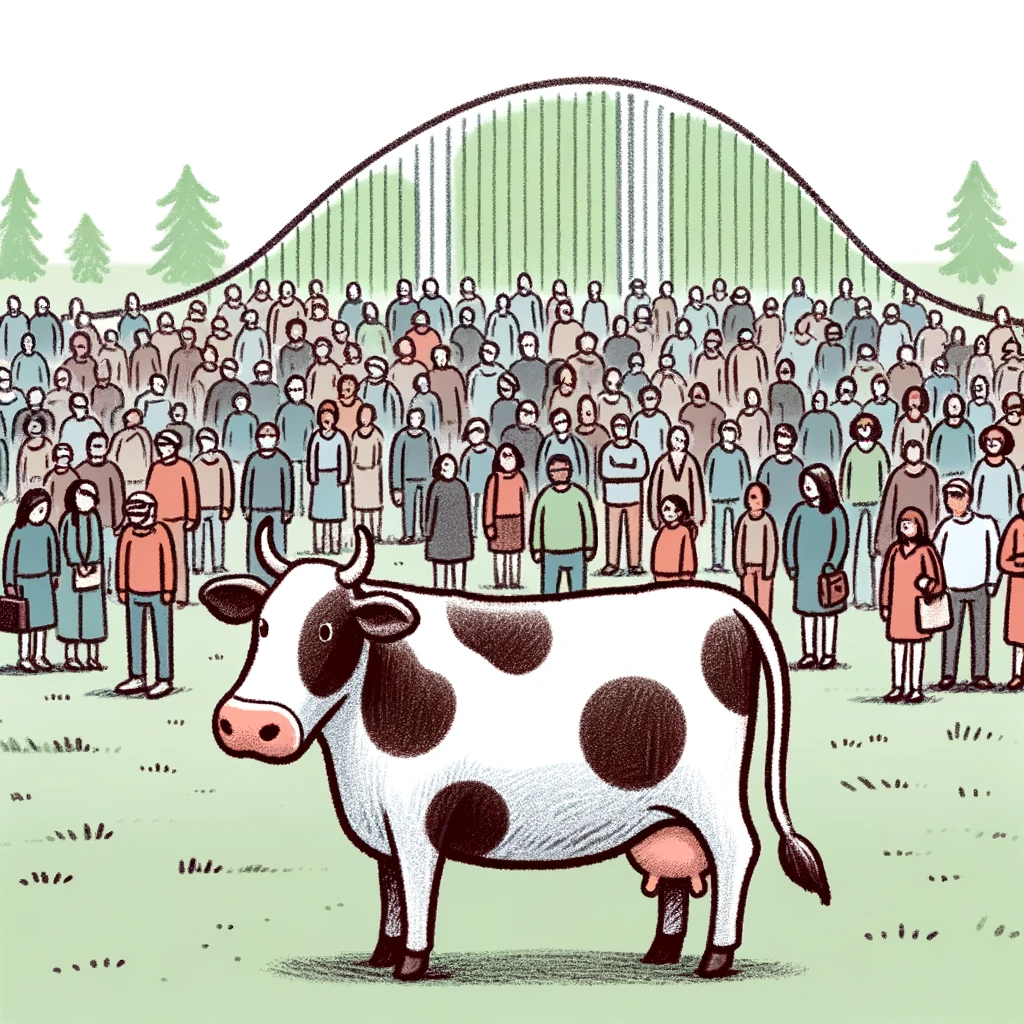
\includegraphics[width=0.5\textwidth]{figures/cow.png}
    \caption[The Wisdom of Crowds]{\textit{\textbf{The Wisdom of Crowds:}} The average of multiple noisy estimates of the weight of a cow is more accurate than any individual estimate. Created with the assistance of DALL·E 2}\label{fig:wisdomofcrowds}
\end{figure}

In this thesis, we will explore Canonical Correlation Analysis, a multiview learning method predicated on the assumption that different \gls{views} provide complementary information about latent variables. The following sections will establish a formal framework for representation learning and motivate the use of Canonical Correlation Analysis in harnessing complementary information from multiview data.

\section{Learning Representations: Definitions and Notation}

Suppose we have a sequence of vector-valued random variables $X\sps{i} \in \R^{D_i}$ for $i \in \{1, \dots, I \}$
We want to learn meaningful $K$-dimensional representations
\begin{equation}
    \label{eq:general-form-of-representations}
    Z\sps{i} = f\sps{i}( X\sps{i}; \theta\sps{i}).
\end{equation}
For convenience, define $D = \sum_{i=1}^I D_i$ and $\theta = \left(\theta\sps{i}\right)_{i=1}^I$.
Without loss of generality take $D_1 \geq D_2 \geq \cdots \geq D_I$.
We will consistently use the subscripts $i,j \in [I]$ for \gls{views};
$d \in [D_i]$ for dimensions of input variables;
and $l,k \in [K]$ for dimensions of representations - i.e. to subscript dimensions of $Z\sps{i}, f\sps{i}$.
Later on we will introduce total number of samples $N$.

In this report, when the functions $f$ are linear, we will typically refer to $u_k$ as \gls{weights}, $Z_k = X_k u_k$ as \gls{representations} or \gls{latent variables} (noting that in the CCA literature they are sometimes referred to as canonical variables \citep{borga_learning_1998}), depending on the context.
We will sometimes consider a matrix $U = \left(u_1, \dots, u_K\right) \in \R^{D \times K}$ of \gls{weights}, and a matrix $Z = \left(Z_1, \dots, Z_K\right) \in \R^{N \times K}$ of representations.
We will refer to the Pearson correlation between features and their respective latent variable $\Corr(X\sps{i}_j, Z_k)$ as the \gls{loadings} of $X\sps{i}_j$ on $Z_k$ \citep{rosipal2005overview, alpert1972interpretation, borga_learning_1998}, noting that the same concept has also been referred to as structure correlations \citep{meredith1964canonical}.

%Covariance matrices
We will use the notation $\Sigma_{ij}=\Cov(X\sps{i}, X\sps{j})$ for the population covariance matrix between the random variables associated with view $i$ and $j$. We will also use $\Sigma_{ii}= \Cov(X\sps{i})$ for the population covariance matrix of the random variables associated with view $i$ with each other.

\subsection{Generalized Eigenvalue Problems in linear algebra}
A Generalized Eigenvalue Problem (GEP) is defined by two symmetric matrices $A,B\in \mathbb{R}^{D\times D}$ \citep{stewart_matrix_1990}\footnote{more generally, $A,B$ can be Hermitian, but we are only interested in the real case}.
They are usually characterized by the set of solutions to the equation:
\begin{align}
    \label{eq:igep}
    Au=\lambda Bu
\end{align}
with $\lambda \in \R, u \in \R^D$, called (generalized) eigenvalue and (generalized) eigenvector respectively.
When $B$ is positive definite, then the GEP becomes equivalent to an eigen-decomposition of the symmetric matrix $B^\mhalf A B^\mhalf$ \citep{ghojogh2019eigenvalue}.
In addition, one can find a basis of eigenvectors spanning $\R^D$.
We define a top-$K$ subspace to be one spanned by some set of eigenvectors {$u_1,\dots,u_K$} with the top-$K$ associated eigenvalues $\lambda_1 \geq \dots \geq \lambda_K$.
We say a matrix $U \in \R^{D \times K}$ defines a top-$K$ subspace if its columns span one.

\paragraph{Uniqueness}
In GEPs, the eigenvectors $u$ are not in general unique, but the generalized eigenvalues $1 \geq \lambda_1 \geq \lambda_2 \geq \dots \geq 0$ are unique \citep{mills1988calculation}.

\subsection{Principal Components Analysis}

Principal Components Analysis \citep{hotelling1933analysis} (\acrshort{pca}) is a classical method in unsupervised machine learning for representation learning.
It is widely used for dimensionality reduction and feature extraction.
The primary goal of \acrshort{pca} is to transform the original high-dimensional data into a new coordinate system defined by orthogonal axes, capturing the most relevant aspects of the data.

In \acrshort{pca}, the representations are constrained to be linear transformations of the form:
\begin{equation}
    \label{eq:pca-linear-function-def}
    Z_k = X u_k,
\end{equation}
where $u_k$ are orthonormal basis vectors such that:
\begin{equation}
    \label{eq:pca-orthonormality-constraint}
    u_k^\top u_k = 1, \quad
    u_k^\top u_l = \delta_{kl} \text{ for } k \neq l.
\end{equation}

The primary goal of \acrshort{pca} is to maximize the variance of the representations \(Z_k\), finding the directions of maximal variance in the data.

\subsubsection{Optimization and Solution}
Mathematically, for the first principal component, this can be formulated as:

\begin{align}
    u_{\text{opt}} & = \underset{u}{\text{argmax}} \left( u^\top \Sigma u \right) \\
    \text{subject to:} \notag                                                     \\
    u^\top u       & = 1 \notag
\end{align}

Where \(\Sigma = \mathbb{E}[X^\top X]\) is the population covariance matrix of the single view data $X$.

The Lagrangian for this problem is:
\begin{equation}
    f(u,\lambda) = u^\top \Sigma u + \lambda(1 - u^\top u),
\end{equation}
where \(\lambda\) is the Lagrange multiplier.
Differentiating the Lagrangian yields the first-order conditions:
\begin{align}
    \Sigma u & = \lambda u, \\
    u^\top u & = 1.
\end{align}

\paragraph{Eigenvalue Problem}

This transforms the problem into an eigenvalue equation for the covariance matrix \(\Sigma\), which can be efficiently solved using standard libraries such as scikit-learn \citep{pedregosa2011scikit}.

The first principal component therefore corresponds to the eigenvector associated with the largest eigenvalue \(\lambda\).
Subsequent components are the remaining eigenvectors ordered by their corresponding eigenvalues.

\subsubsection{Limitations}
There are two major limitations of \acrshort{pca} that are relevant to this thesis.
The first is revealed by the epigraph of this chapter, which highlights the fact that \acrshort{pca} is not scale invariant.
This means that the principal components are sensitive to the scale of the data, and therefore the units in which the data is measured.
Furthermore, the interpretation of the principal components is challenging; they are linear combinations of all of the original features. For this reason, sparse variants of \acrshort{pca} have been developed \citep{zou2006sparse,zou2018selective}, which aim to find sparse linear combinations of the original features; interpretable as a subset of the original features contributing to a significant proportion of the variance in the data.
Another major limitation of \acrshort{pca} in the context of multiview learning is that it does not explicitly take advantage of either the redundancy or the complementary information in multiview data, even if we concatenate the views into a single random variable $X$.
Nevertheless, \acrshort{pca} remains a popular tool in practice \citep{greenacre2022principal} and is a useful baseline for multiview learning methods, and we will use it as a point of comparison throughout this thesis.

\subsection{Partial Least Squares}

Partial Least Squares (PLS) \citep{wold1975path} aims to maximize the shared covariance between two paired sets of data, referred to as \gls{views}. \acrshort{pls} can be seen as a generalization of \acrshort{pca}, where \acrshort{pca} becomes a special case when the two \gls{views} are identical.

\acrshort{pls} optimises for the dot product between the two views, a measure of similarity.

\begin{align}
    \label{eq:dot-product}
    \langle X\sps{1}u^{(1)}, X\sps{2}u^{(2)} =\sqrt{u\spsT{1}\Sigma_{11}u\sps{1}} \sqrt{u\spsT{2}\Sigma_{22}u\sps{2}} \cos(\theta)
\end{align}

Where $\theta$ is the angle between the two representations.
In order to constrain the problem, we set the norms of the weights to 1.

\subsubsection{Optimization and Solution}

The constrained optimization problem for \acrshort{pls} can therefore be formulated as:

\begin{align}
    u\sps{1}_{\text{opt}} & = \underset{u\sps{1}}{\mathrm{argmax}} \{ u\spsT{1} \Sigma_{12} u\sps{2} \} \\
    \text{subject to:} \notag                                                                             \\
    u\spsT{1}u\sps{1}   & = 1 \notag                                                                    \\
    u\spsT{2}u\sps{2}   & = 1 \notag
\end{align}

The Lagrangian for this optimization problem can be formulated as:

\begin{equation}
    f(u\sps{1}, \lambda) = u\spsT{1} \Sigma_{12} u\sps{2} + \lambda_1 (1 - u\spsT{1}u\sps{1}) + \lambda_2 (1 - u\spsT{2}u\sps{2})
\end{equation}

Upon deriving the first order conditions, we get:

\begin{align}
    \Sigma_{21} u\sps{1} & = \lambda_2 u\sps{2} \\
    \Sigma_{12} u\sps{2} & = \lambda_1 u\sps{1} \\
    u\spsT{1}u\sps{1}  & = 1                  \\
    u\spsT{2}u\sps{2}  & = 1
\end{align}

By substituting the constraint conditions into these equations, we find that \( \lambda_1 = \lambda_2 = \lambda \) by symmetry. Further simplification yields:

\begin{align}
    \Sigma_{21} \Sigma_{12} u\sps{2} & = \lambda^2 u\sps{2} \\
    \Sigma_{12} \Sigma_{21} u\sps{1} & = \lambda^2 u\sps{1}
\end{align}

\paragraph{Eigenvalue Problem}

Once again, we see that solving these equations will yield the \( u\sps{1} \) and \( u\sps{2} \) vectors as eigenvectors, this time of \( \Sigma_{12} \Sigma_{21} \) and \( \Sigma_{21} \Sigma_{12} \), respectively \citep{hoskuldsson1988pls}.

\paragraph{Generalized Eigenvalue Problem}

We can also represent the system of equations in matrix form as follows:

\begin{align}
    \begin{pmatrix}
        0           & \Sigma_{12} \\
        \Sigma_{21} & 0
    \end{pmatrix}
    \begin{pmatrix}
        u\sps{1} \\
        u\sps{2}
    \end{pmatrix}
    =
    \lambda
    I
    \begin{pmatrix}
        u\sps{1} \\
        u\sps{2}
    \end{pmatrix}
\end{align}

Which is of the form $A v = \lambda B v$. \acrshort{pls} is therefore also defined by the solution to a single generalized eigenvalue problem.

Given the notions of uniqueness in GEPs, the weights $u$ are not in general unique but we can write the vector of generalized eigenvalues $(\lambda_1, \dots, \lambda_K)$ representing covariances as:

\begin{align}
    \label{eq:pls-vector-of-correlations-def}
    \PLS_K(X^{(1)},X^{(2)}) \defeq (\lambda_k)_{k=1}^K
\end{align}

\subsubsection{Limitations} Like \acrshort{pca}, a major problem with applying \acrshort{pls} to neuroimaging and behavioural modalities is that \acrshort{pls} is not scale invariant.
This is because the dot product in equation~\ref{eq:dot-product} is not scale invariant since it is not normalized by the norms of the representations.
Since representations with larger norms will have larger dot products, \acrshort{pls} is biased towards larger representations.
It is therefore also biased towards the largest principal components in the data \citep{helmer2020stability}.
This is particularly problematic when there is a low signal to noise ratio since \acrshort{pls}.
Like \acrshort{pca}, another issue is the lack of sparsity in the \acrshort{pls} solution which has been an active area of research \citep{chun2010sparse, witten2009penalized}.

\subsection{Canonical Correlation Analysis}\label{sec:cca}

In Canonical Correlation Analysis (\acrshort{cca}), we aim to find the directions that maximize correlation, as opposed to maximizing covariance between two \gls{views} of a dataset.
This can be viewed as maximizing the cosine similarity between the two views, rather than the dot product, as in \acrshort{pls}.
Rearranging equation~\ref{eq:dot-product} yields:

\begin{align}
    \label{eq:cosine-similarity}
    \cos(\theta) = \frac{\langle X\sps{1}u^{(1)}, X\sps{2}u^{(2)}}{\sqrt{\langle X\sps{1}u^{(1)}, X\sps{1}u^{(1)}}\cdot \sqrt{\langle X\sps{2}u^{(2)}, X\sps{2}u^{(2)}}}= \frac{u\spsT{1}\Sigma_{12}u\sps{2}}{\sqrt{u\spsT{1}\Sigma_{11}u\sps{1}} \sqrt{u\spsT{2}\Sigma_{22}u\sps{2}}}
\end{align}

and we can see that the dot product from equation~\ref{eq:dot-product} is normalised by the inner products so that \acrshort{cca} is scale invariant, unlike \acrshort{pls}.
All that matters is the angle between the representations, not their magnitude.
Once again, in order to constrain the problem, we this time set the norms of the representations to 1.

\subsubsection{Optimization and Solution}
The optimization problem for \acrshort{cca} can be expressed as:

\begin{align}
    & u_{\text{opt}}=\underset{u}{\mathrm{argmax}}\{ u\spsT{1}X\spsT{1}X\sps{2}u\sps{2} \} \\
    & \text{subject to:} \notag                                                                \\
    & u\spsT{1}\Sigma_{11}u\sps{1}=1 \notag                                                  \\
    & u\spsT{2}\Sigma_{22}u\sps{2}=1 \notag
\end{align}

Although non-convex, numerous methods exist for solving the \acrshort{cca} problem, including eigendecomposition and generalized eigendecomposition solvers \citep{uurtio2017tutorial} and block coordinate descent via alternating least squares regressions \citep{golub1995canonical,sun2008least}.

The first-order conditions derived in the same manner as the \acrshort{pls} case are:

\begin{align}
    \label{CCA:FOCs}
    & \Sigma_{21}u\sps{1}=\lambda\sps{2} \Sigma_{22}u\sps{2} \\
    & \Sigma_{12}u\sps{2}=\lambda\sps{1} \Sigma_{11}u\sps{1} \\
    & u\spsT{1}\Sigma_{11}u\sps{1}=1                       \\
    & u\spsT{2}\Sigma_{22}u\sps{2}=1
\end{align}

\paragraph{Eigenvalue Problems}

Substituting the second two conditions into the first two, we get \(\lambda\sps{1}=\lambda\sps{2}=\lambda\). Finally, substituting the first two conditions into each other, we find the eigenvalue problems:

\begin{align}\label{eq:cca-eigenvalue-problems}
    & \Sigma_{11}^{-1}\Sigma_{12}\Sigma_{22}^{-1}\Sigma_{21}u\sps{1}=\lambda^2u\sps{1} \\
    & \Sigma_{22}^{-1}\Sigma_{21}\Sigma_{11}^{-1}\Sigma_{12}u\sps{2}=\lambda^2u\sps{2}
\end{align}

An alternative form of the \acrshort{cca} problem can be developed by reparameterizing \(u\sps{i*}=\Sigma_{ii}^{-\frac{1}{2}}u\sps{i}\). The optimization problem then becomes:

\begin{align}\label{eq:cca-reparameterized}
    & u_{\text{opt}}=\underset{u}{\mathrm{argmax}}\{ u\spsT{1}\Sigma_{11}^{-\frac{1}{2}}\Sigma_{12}\Sigma_{22}^{-\frac{1}{2}}u\sps{2} \} \\
    & \text{subject to:} \notag                                                                                                            \\
    & u\spsT{1}u\sps{1}=1 \notag                                                                                                         \\
    & u\spsT{2}u\sps{2}=1 \notag
\end{align}

This reparameterized form will later underpin Deep Canonical Correlation Analysis (\acrshort{dcca}) through the matrix $T=\Sigma_{11}^{-\frac{1}{2}}\Sigma_{12}\Sigma_{22}^{-\frac{1}{2}}$.
This form also shows that \acrshort{pls} and \acrshort{cca} can be made equivalent by whitening the data matrices before constructing the covariance matrix.
When the number of features exceeds the number of samples (\(p>n\)), \acrshort{cca} becomes degenerate because the within-view covariance matrices cannot be inverted—contrasting with \acrshort{pls}, which is always computable.

\paragraph{Generalized Eigenvalue Problem}

We can also represent the system of equations in equation~\ref{CCA:FOCs} as a matrix equation:

\begin{align}
    \begin{pmatrix}
        0           & \Sigma_{12} \\
        \Sigma_{21} & 0
    \end{pmatrix}
    \begin{pmatrix}
        u\sps{1} \\
        u\sps{2}
    \end{pmatrix}
    =
    \lambda
    \begin{pmatrix}
        \Sigma_{11} & 0           \\
        0           & \Sigma_{22}
    \end{pmatrix}
    \begin{pmatrix}
        u\sps{1} \\
        u\sps{2}
    \end{pmatrix}
\end{align}

Which is once again of the form $A u = \lambda B u$. \acrshort{cca}, like \acrshort{pls}, is therefore also defined by the solution to a single generalized eigenvalue problem.

\paragraph{Canonical Correlations}
In the case of \acrshort{cca}, the generalized eigenvalues $\lambda$ are generally called canonical correlations \citep{hotelling1935canonical, hotelling1992relations}.
Given the notions of uniqueness in GEPs, the weights $u$ are not in general unique but we can write the vector of generalized eigenvalues or canonical correlations as:
\begin{align}
    \label{eq:cca-vector-of-correlations-def}\small
    \CCA_K(X^{(1)},X^{(2)}) \defeq (\rho_k)_{k=1}^K
\end{align}

\subsubsection{Limitations}

A major limitation of \acrshort{cca} is revealed by the forms in equations \ref{eq:cca-eigenvalue-problems} and equation~\ref{eq:cca-reparameterized}; \acrshort{cca} in general requires the inversion of covariance matrices, which is computationally expensive, potentially numerically unstable, and impossible when the number of features exceeds the number of samples such that the covariance matrices are not full rank.

\subsection{Multiview \acrshort{cca}}

Multiview \acrshort{cca} or \acrshort{mcca} is a straightforward extension of \acrshort{cca} to the case of 3-or more datasets.
The goal is to find a set of directions \(u\sps{i}\) such that the pairwise correlations between the views are maximized.

\subsubsection{Optimization and Solution}

The optimization problem for \acrshort{mcca} can be stated as:
\begin{align}
    & u_{\text{opt}} = \underset{u}{\mathrm{argmax}} \sum_{i=1}^{m} \sum_{j=1, j \neq i}^{m} u\spsT{i} \Sigma_{ij} u\sps{j} \\
    & \text{subject to:} \notag                                                                                               \\
    & \sum_{i=1}^{m} u\spsT{i} \Sigma_{ii} u\sps{i} = 1 \notag
\end{align}

\paragraph{Generalized Eigenvalue Problem}

The generalized eigenvalue problem (GEP) for MCCA can be written in matrix form as follows:

\begin{align}
    \small
    \begin{pmatrix}
        0           & \Sigma_{12} & \cdots & \Sigma_{1m} \\
        \Sigma_{21} & 0           & \cdots & \Sigma_{2m} \\
        \vdots      & \vdots      & \ddots & \vdots      \\
        \Sigma_{m1} & \Sigma_{m2} & \cdots & 0
    \end{pmatrix}
    \begin{pmatrix}
        u\sps{1} \\
        u\sps{2} \\
        \vdots   \\
        u\sps{m}
    \end{pmatrix}.
    =
    \lambda
    \begin{pmatrix}
        \Sigma_{11} & 0           & \cdots & 0           \\
        0           & \Sigma_{22} & \cdots & 0           \\
        \vdots      & \vdots      & \ddots & \vdots      \\
        0           & 0           & \cdots & \Sigma_{mm}
    \end{pmatrix}
    \begin{pmatrix}
        u\sps{1} \\
        u\sps{2} \\
        \vdots   \\
        u\sps{m}
    \end{pmatrix}.
\end{align}

This GEP formulation of MCCA can be presented in a unified framework generalizing CCA and ridge-regularized extensions. Indeed, we now take $A,B_\alpha \in \R^{D \times D}$ to be block matrices $A = (A\sps{ij})_{i,j=1}^I, B_\alpha = (B_\alpha\sps{ij})_{i,j=1}^I$ where the diagonal blocks of $A$ are zero, the off-diagonal blocks of $B_\alpha$ are zero, and the remaining blocks are defined by:
\begin{align}
    \label{eq:gep-most-general-formulation}%\small
    A^{(ij)} &= \Cov(X\sps{i}, X\sps{j}) \text{ for } i \neq j, \quad % \text{ for } i,j \in [I], ; \:\:
    B_\alpha^{(ii)} = \alpha_i I_{D\sps{i}} + (1-\alpha_i) \Var(X\sps{i})  %\text{ for } i \in [I]
\end{align}
Where $\alpha \in [0,1]^I$ is a vector of ridge penalty parameters: taking $\alpha_i = 0 \: \forall i$ recovers CCA and $\alpha = 1 \: \forall i$ recovers PLS.
We may omit the subscript $\alpha$ when $\alpha=0$ and we recover the `pure CCA' setting; in this case, following \ref{eq:cca-vector-of-correlations-def} we can define

\begin{align}
    \MCCA_K(X\sps{1},\dots,X\sps{I})
\end{align}

to be the vector of the top-$K$ generalized eigenvalues which are the average of the top-$K$ correlations between each pair of views.

\subsection{Linear Discriminant Analysis LDA}

Linear Discriminant Analysis (LDA) can be viewed as a special case of Canonical Correlation Analysis (CCA) where \(X^{(2)}\) is a one-hot encoded matrix representing the class labels.
This allows us to draw a connection between the unsupervised learning framework of \acrshort{cca} and the supervised framework of LDA\citep{balakrishnama1998linear,riffenburgh1957linear}, thus expanding the understanding of both algorithms.

\textbf{Intuition:} In LDA, the aim is to find a lower-dimensional subspace where the classes are maximally separated. This objective can be viewed through the lens of \acrshort{cca}, where the optimal directions \(u^{(1)}\) and \(u^{(2)}\) in the original and one-hot encoded spaces aim to maximize correlation. In the LDA context, \(u^{(1)}\) would maximize the separation between classes.

\subsubsection{Optimization and Solution}

Mathematically, LDA is reduced to solving a generalized eigenvalue problem involving the between-class scatter matrix \(S_B\) and the within-class scatter matrix \(S_W\):

\[
    \hat{S_B} = \sum_{i=1}^{c} n_i (\mu_i - \mu)(\mu_i - \mu)\top
\]

\[
    \hat{S_W} = \sum_{i=1}^{c} \sum_{x \in X_i} (x - \mu_i)(x - \mu_i)\top
\]

\textbf{Connection to \acrshort{cca}:} When \(X^{(2)}\) is the one-hot encoded matrix of class labels, the \acrshort{cca} problem effectively tries to maximize the correlation between the feature vectors and their corresponding labels.
This turns out to be equivalent to maximizing the between-class variance in LDA while minimizing the within-class variance.
Thus, LDA can be thought of as a constrained form of \acrshort{cca}, tailored to classification tasks.

This perspective unifies the two algorithms and shows that the core objective—finding meaningful relationships or directions in the data—is shared between both \acrshort{cca} and LDA.

\subsection{Sample Covariance and Population Covariance}
In the previous sections, the methods were described in terms of population covariance matrices such as \(\Sigma_{11}=\mathbb{E}[X\spsT{1} X\sps{1}]\), \(\Sigma_{22}=\mathbb{E}[X\spsT{2} X\sps{2}]\), and \(\Sigma_{12}=\mathbb{E}[X\spsT{1} X\sps{2}]\).
These population covariances assume an underlying probability distribution from which the data are drawn.

\textbf{Sample Covariance:} In practical settings, we often do not have access to the entire population but only to a sample. Hence, we can use the Sample Average Approximation to estimate these covariances:

\[
    \hat{\Sigma}\sps{12} = \frac{1}{b-1} \bar{\mathbf{X}\sps{1}} \bar{\mathbf{X}\sps{2}}\top
\]

Here, \(b\) denotes the size of the minibatch, and \(\mathbf{X}\sps{1} \in \mathbb{R}^{p \times b}\) and \(\mathbf{X}\sps{2} \in \mathbb{R}^{q \times b}\) are the data matrices for the samples from \(X\sps{1}\) and \(X\sps{2}\), respectively. The bar over \(\mathbf{X}\sps{1}\) and \(\mathbf{X}\sps{2}\) signifies that these are centered versions of the matrices, i.e., the mean has been subtracted from each column.
For the ease of both reader and writer, we will drop the bars for the remainder of the thesis and assume that the data are always centered without loss of generality.

\textbf{Practical Implications:} Using sample covariance matrices introduces some estimation error but allows us to apply the methods in real-world scenarios where population-level data are unattainable.
Additionally, the use of minibatches (chunks of data) in later chapters provides a computationally efficient way to estimate these covariances in large-scale problems, at the cost of some additional statistical noise.

\textbf{Connection to Previous Methods:} The use of sample covariance matrices is directly applicable to algorithms like \acrshort{cca} and LDA. When replacing the population covariances \(\Sigma\sps{ij}\) with sample estimates, the optimization problems remain structurally similar but are solved using the sample data.

This dual perspective—considering both population and sample covariance matrices—enables a more robust and flexible approach to the methods discussed, bridging the gap between theoretical analysis and practical application.
It will be particularly useful in the context of chapter \ref{ch:loadings} where we will use population variables as ground truth while estimating the models using sample data.


\section{Practical Frameworks for Evaluating Multiview Learning Methods}

At this point, we have introduced the theoretical foundations of multiview learning, and a number of classical representation learning algorithms including \acrshort{cca} and its variants.
However, it is not yet clear how we should evaluate these methods in practice.
In this section, we compare the machine learning and the statistical approach of permutation testing.
These two approaches are not mutually exclusive, and statistical learning theory has emerged as a unifying framework for both perspectives \citep{vapnik1999nature, hastie2009elements}.

\subsubsection{Permutation Testing}

\begin{figure}
    \centering
    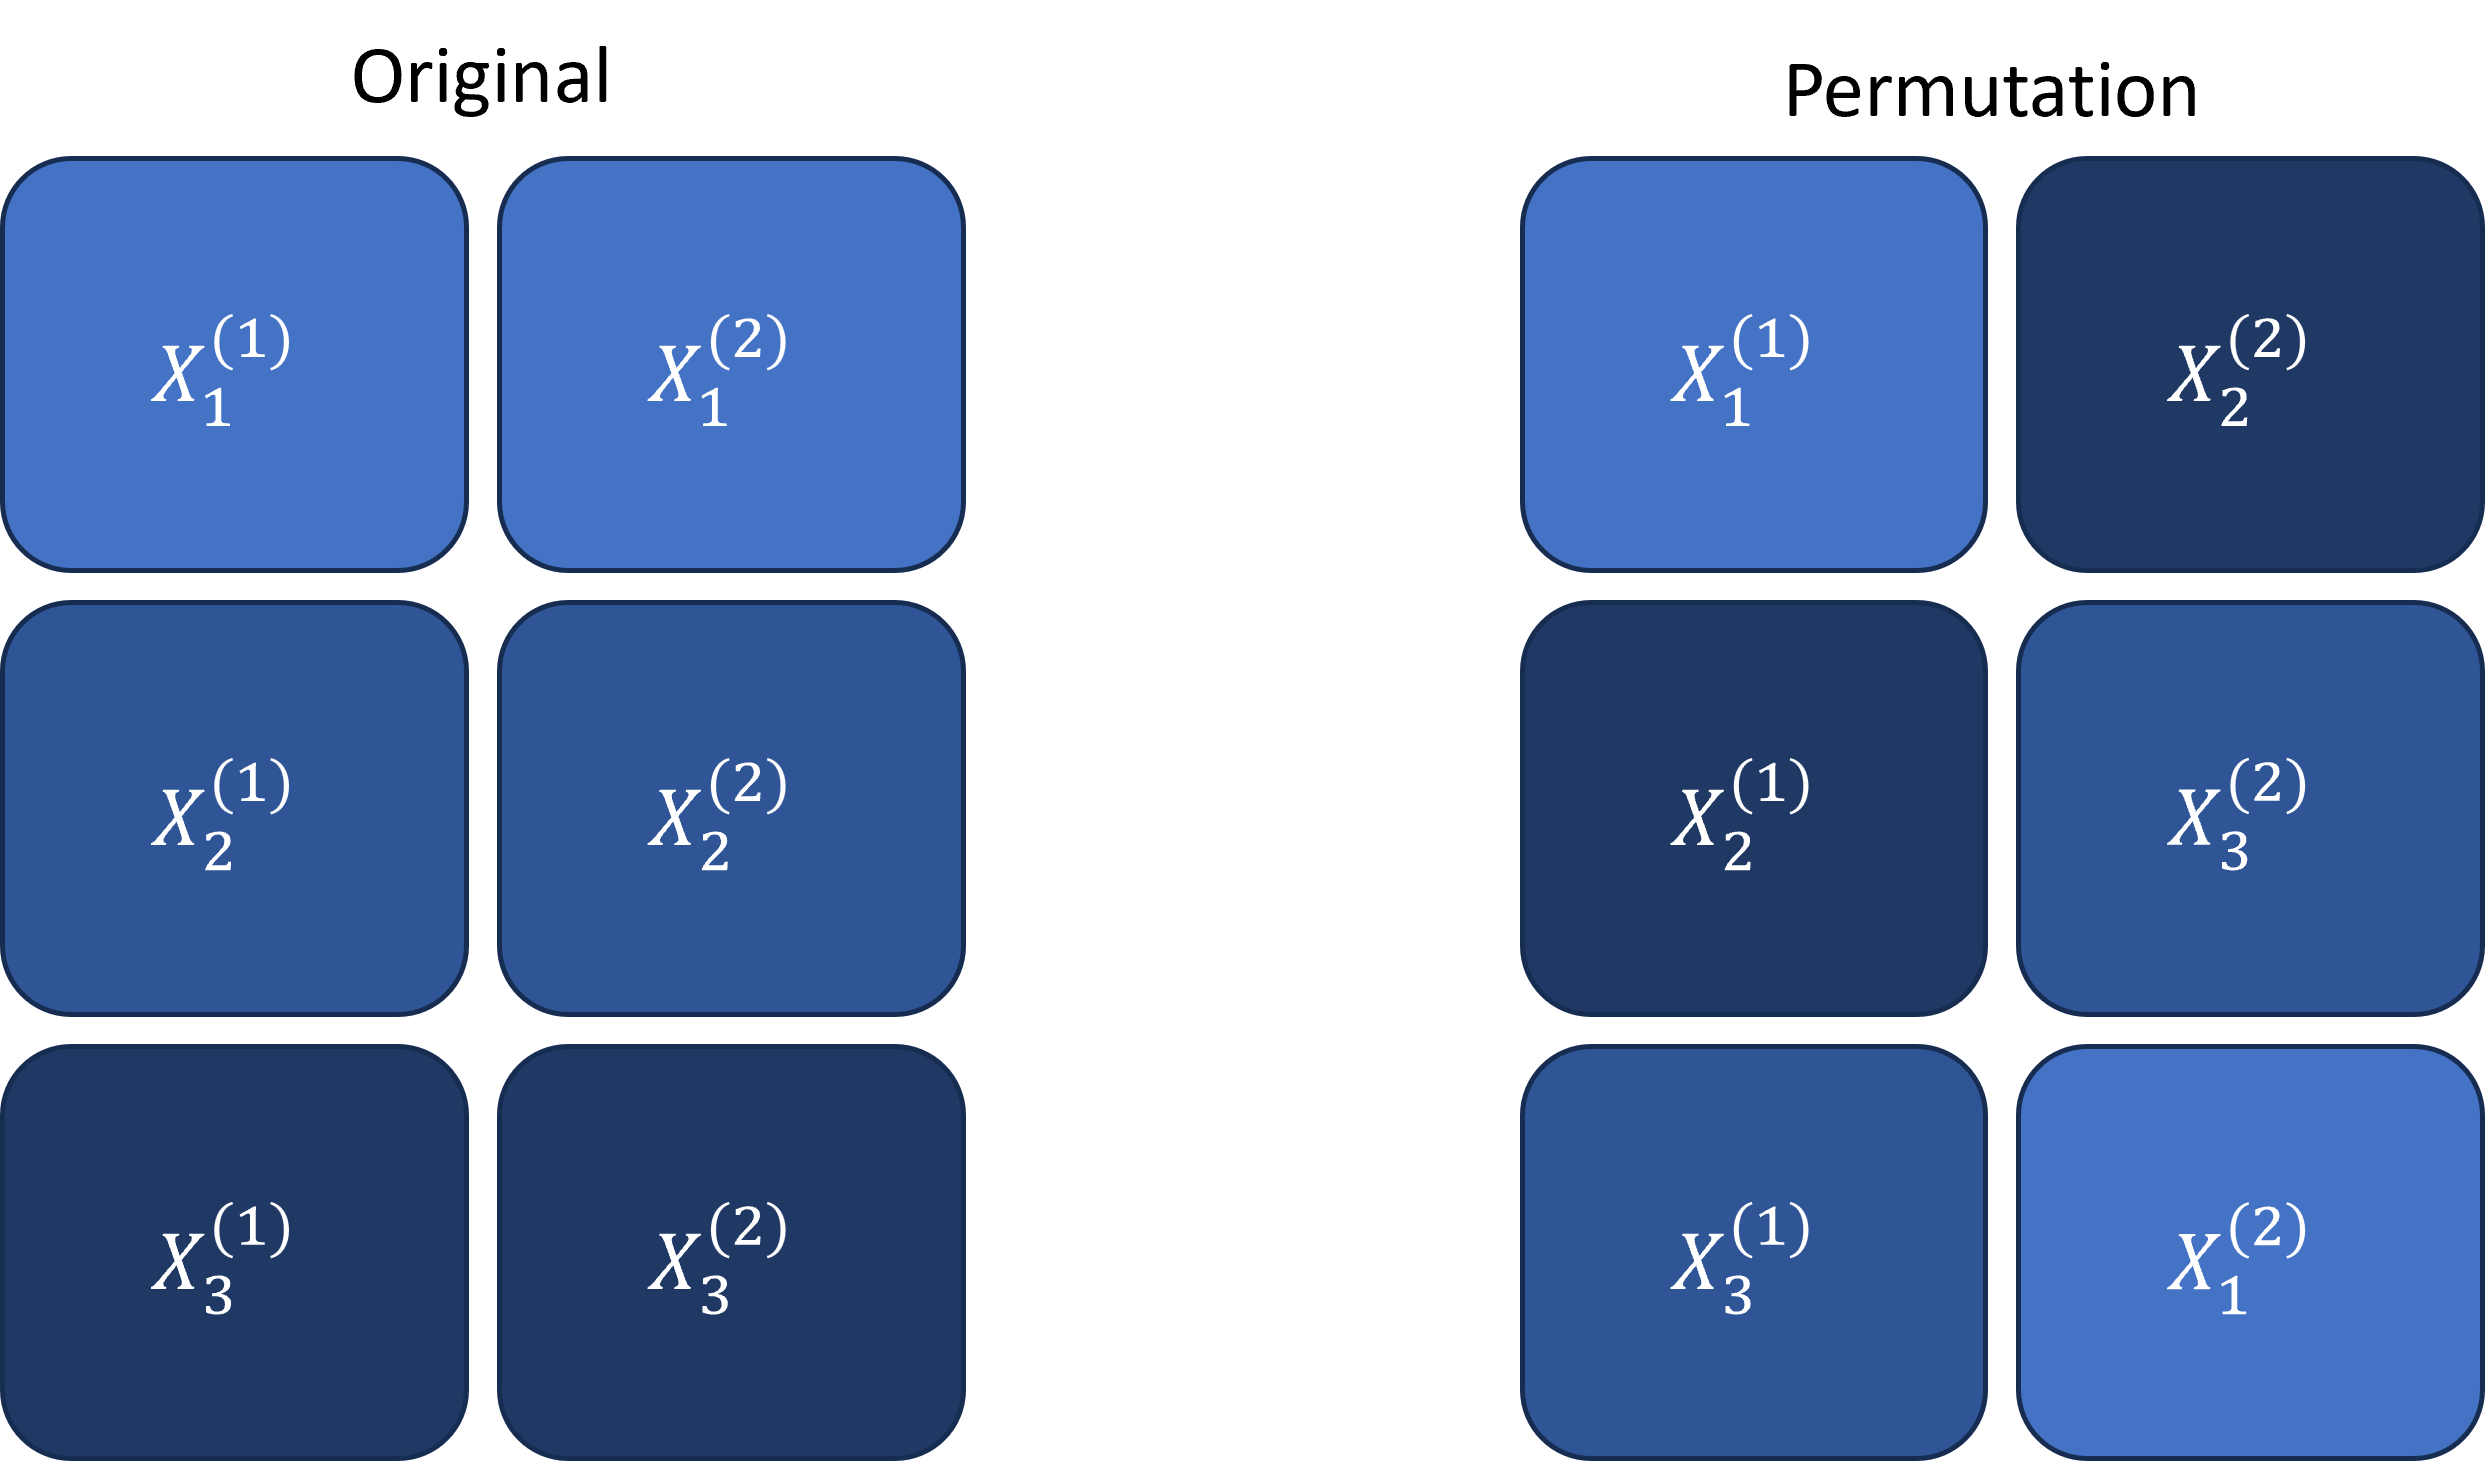
\includegraphics[width=0.8\textwidth]{figures/permutation_test.png}
    \caption{Schematic of the permutation testing procedure. The original data are randomly shuffled, and the model is retrained on the shuffled data. This process is repeated multiple times, and the model's performance on the original data is compared to the distribution of performances on the shuffled data.}
    \label{fig:statistical-inference}
\end{figure}

Permutation testing offers a robust way to evaluate the significance of the results obtained by multiview learning methods and, for a single component, is a relatively simple process \citep{winkler2020permutation}.
As illustrated in Figure~\ref{fig:statistical-inference}, the views are randomly and separately shuffled, and the model is then trained and tested on this permuted data.
This process is repeated multiple times, generating a distribution of performance metrics under the null hypothesis, where there is no relationship between the views.
The actual performance of the model on the unshuffled data is then compared to this distribution.
If the actual performance is significantly better than the permuted performance, it suggests that the model is capturing meaningful relationships in the data.

\subsubsection{Machine Learning}

\begin{figure}
    \centering
    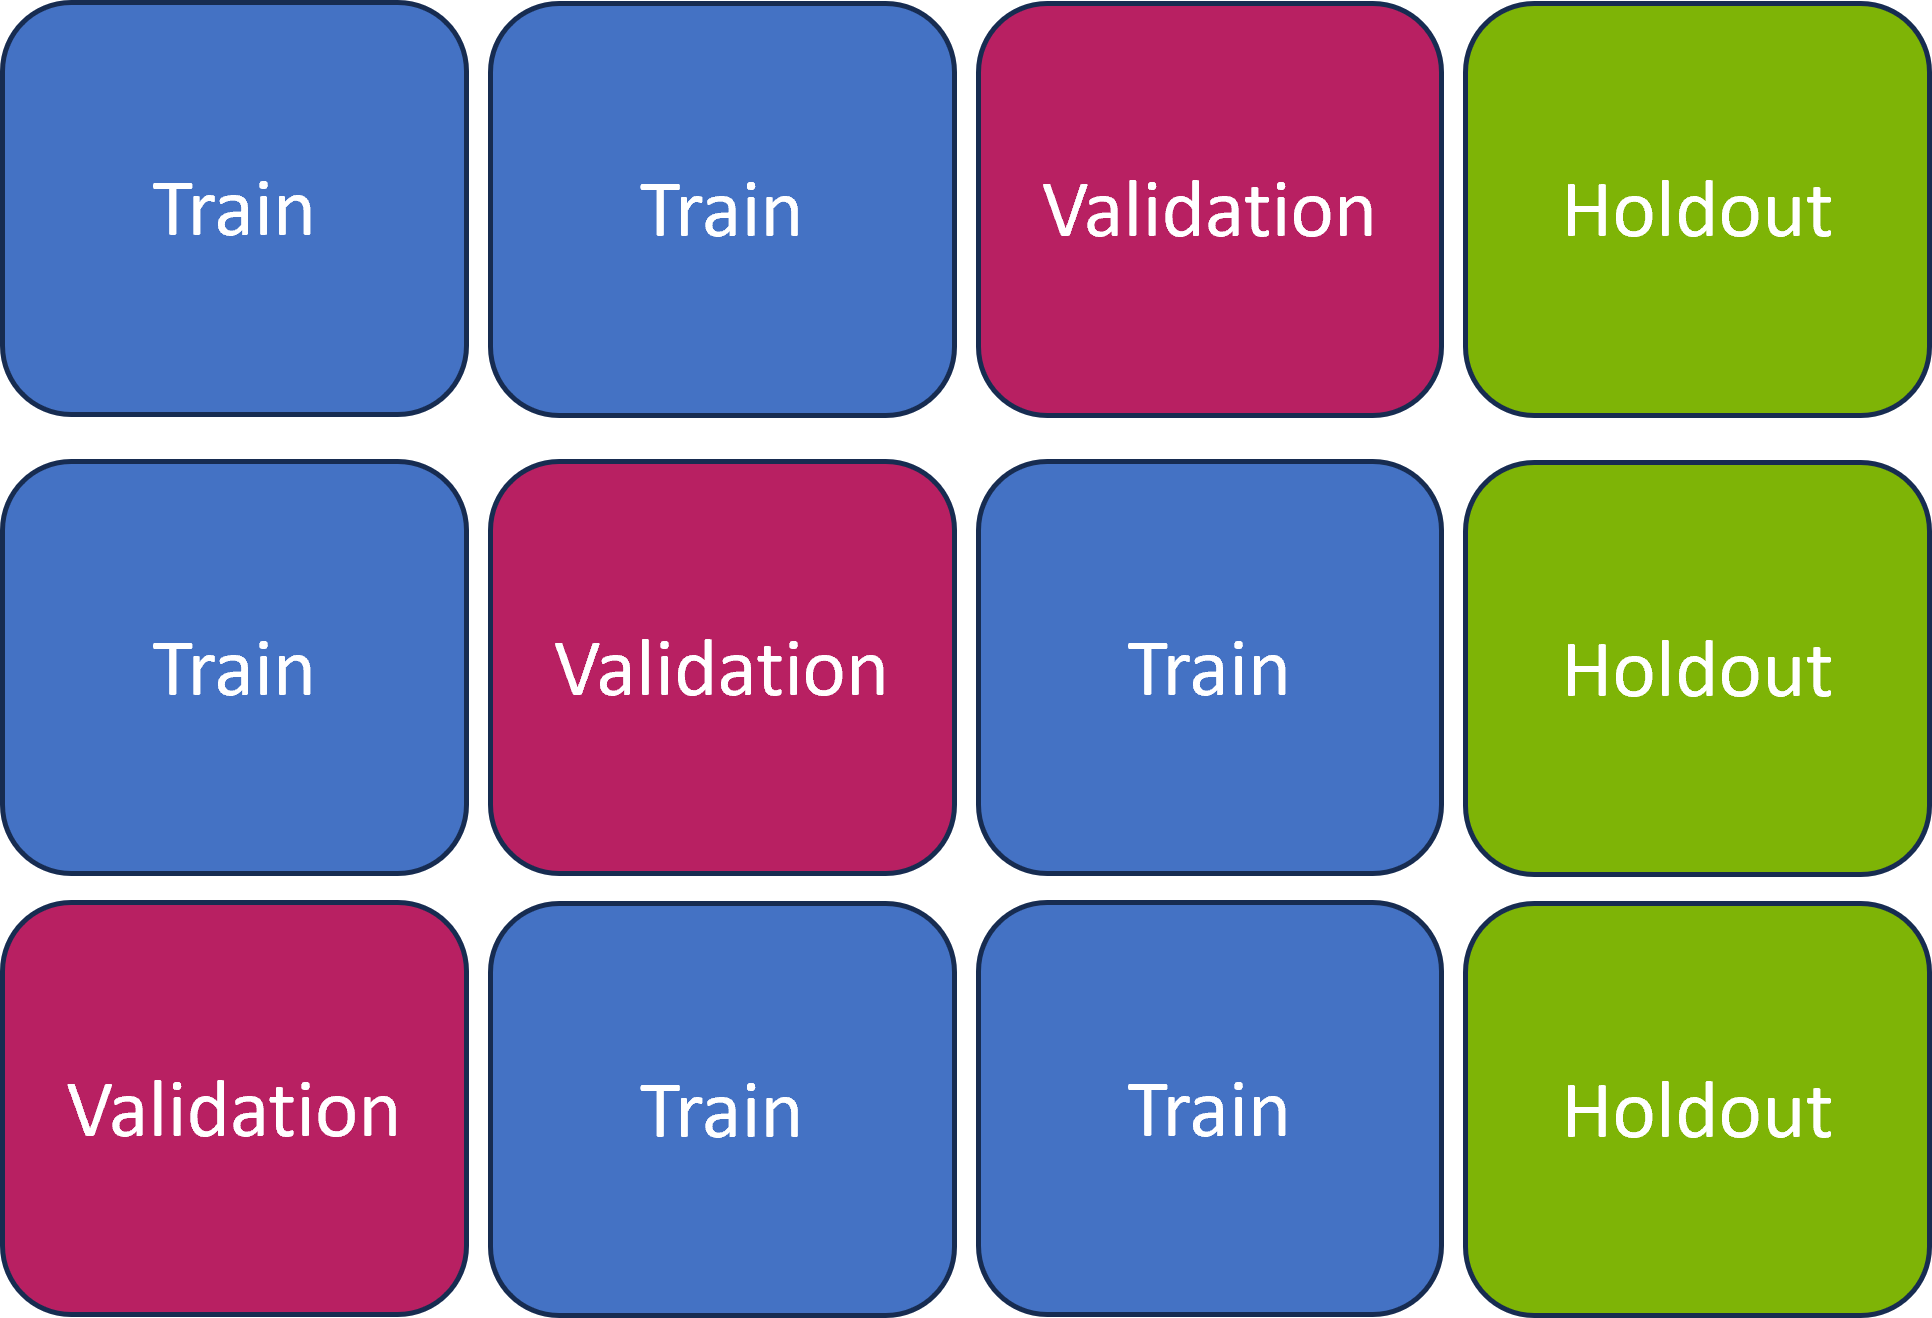
\includegraphics[width=0.8\textwidth]{figures/cross-validation.png}
    \caption{Schematic of the cross-validation procedure. The original data are partitioned into training and test sets. In cross-validation, the training set is further partitioned into training and validation sets. The model is trained on the training set and evaluated on the validation set for different parameter values. The parameter value with the best performance on the validation set is selected, and the model is retrained on the entire training set. The final model is evaluated on the single test or holdout set.}
    \label{fig:machine-learning}
\end{figure}

The machine learning approach to evaluating multiview learning methods is to use a holdout or test set to estimate the out-of-sample performance of the model.
Within the training set, where necessary, cross-validation is used to select the best model hyperparameters.
Cross-validation involves partitioning the training set into training and validation sets, training the model on the training set, and evaluating the model on the validation set.
When this is performed for multiple subsets of the training set, it is referred to as \(k\)-fold cross-validation as illustrated in figure \ref{fig:machine-learning}.
The model hyperparameters are then selected based on the performance across the validation sets.
The model is then retrained on the entire training set using the best hyperparameters, and evaluated on the test set.

In this thesis, we will use the machine learning approach throughout.
This is because in scaling up to large datasets, permutation testing becomes computationally intractable.
This is because permutation testing requires retraining the model multiple times on the permuted data.
This comes at the cost of only being able to evaluate models with a point estimate of performance, rather than a distribution.
In chapter \ref{ch:loadings}, we observe and argue that signals of interest have a large effect size, and therefore permutation testing is not necessary to evaluate the significance of the results.

\subsection{Components and Subspaces in CCA}

\subsubsection{Eigenvalue Problems in CCA}

While our focus so far has primarily been on the top-1 eigenvector-eigenvalue pair, it's important to note that the methodology also extends to the top-k subspace problem. This broader approach involves identifying the top-k eigenvectors and their corresponding eigenvalues.

\subsubsection{Addressing the Top-k Problem}

Transitioning from a focus on the top-1 component to exploring the top-k subspace introduces additional complexities. One common method to solve the top-k problem is to identify the top-1 component and then apply a deflation process to find subsequent orthogonal components.
Deflation involves removing the top-1 component from the data and then repeating the process to find the next top-1 component. This process is repeated until the desired number of components is found.
For instance, Hotelling's Deflation \citep{hotelling1933analysis} involves removing the top-1 component from the data, while Projection Deflation \citep{mackey2008deflation} involves projecting the data onto the orthogonal complement of the top-1 component.
Different deflation methods enforce different forms of orthogonality, which can impact the resulting components and their interpretation, particularly when the first component is not a true eigenvector.

\subsubsection{Non-Uniqueness of Components}

Furthermore, non-uniqueness is a significant challenge in representation learning, particularly when eigenvectors have repeated eigenvalues. Imagine a scenario where the top-1 eigenvalue is repeated \(k\) times. In this case, there are \(k\) possible eigenvectors that can be associated with the top-1 eigenvalue. While this is unlikely to occur in practice, the eigenvalues can in practice be very close to each other, leading to numerical instability and non-uniqueness in the components. Particularly true in cross-validation settings, this non-uniqueness can lead to instability in the components, complicating their interpretation and comparison.
For example, the top-1 component in one analysis might be the second component in another analysis, making it difficult to compare the results.

This non-uniqueness also has a grounding in the probabilistic perspectives on PCA and CCA (introduced in chapter \ref{ch:loadings}), where the latent variables are considered unique only up to a rotation.
This perspective further reinforces the subspace approach, emphasizing the identification of a subspace rather than specific directions within it.

\paragraph{Thesis Approach: Concentrating on the Top-1 Component}

In this thesis, we focus on the top-1 component in CCA to align with and facilitate comparison with typical componentwise studies in brain-behavior research.
This choice is driven by the complexity associated with the top-k problem and the variety of methods available to address it.
Under the assumption of a significant eigengap\footnote{An `eigengap' refers to the difference in magnitude between consecutive eigenvalues in an eigenvalue problem. A significant eigengap between the first and second eigenvalues suggests that the first eigenvalue (and its corresponding eigenvector) is distinctly more significant than the next, lending credence to its uniqueness and importance.}, the first component can be considered equivalent to the top-1 subspace.
This equivalence allows for a clear and interpretable analysis, making the top-1 subspace a straightforward and reliable choice for studying multivariate data.
It is important to note that while we focus on the top-1 component, the later sections of the thesis introduce a method for simultaneously solving the complete subspace, addressing broader subspace analyses.


\section{Multiview Learning in Neuroimaging}

Finally, we review important applications of multiview learning from the literature in neuroimaging, which will be our reference in chapters \ref{ch:als} and \ref{ch:loadings}.

\subsection{Multiview Data in Neuroscience and Genetics}

In neuroscience and genetics, two specific types of multiview studies are particularly relevant to this thesis: brain-behavior studies and imaging-genetics.
Both involve the integration of data from multiple sources, offering rich insights into complex phenomena.

Brain-behavior studies typically involve pairing neuroimaging data, such as that obtained from Structural MRI (sMRI) or Functional MRI (fMRI), with non-imaging data like responses from questionnaires, cognitive test results, and other behavioral assessments.
sMRI provides detailed anatomical brain images, essential for understanding brain structure and neurological disorders \citep{kanai2011structural}, while fMRI focuses on brain function by mapping activity during cognitive tasks \citep{miranda2021systematic}.
The integration of these imaging techniques with behavioral data offers a comprehensive view of how brain structures and functions correlate with behavioral and cognitive patterns \citep{rypma2001age,genon2022linking}.

Imaging-Genetics, another critical multiview approach, combines neuroimaging data with genetics and omics information \citep{le2008sparse}.
This interdisciplinary field seeks to understand the genetic influences on brain structure and function, thereby illuminating the genetic basis of neuropsychiatric disorders and cognitive traits \citep{bogdan2017imaging}.
Studies in this area can explore how specific genetic variations correlate with differences in brain morphology or activity patterns observed in neuroimaging \citep{liu2014review}.

Together, these multiview approaches are fundamental in advancing our understanding of the brain's structure, function, and its interactions with genetic and behavioral factors.
They represent key applications of SSL in neuroscience and genetics, providing comprehensive insights that underpin developments in these fields.

\subsection{Applications of Multiview Learning in Neuroimaging}

There have been a number of applications of \acrshort{cca} and related methods to multiview problems in neuroimaging.
Using resting state fMRI data, modes of correlation have been found that relate to differences in sex and age relating to drug and alcohol abuse, depression and self harm \citep{mihalik2019brain}.
A similar mode relating to `positive-negative' wellbeing has been found across studies \citep{smith2015positive} suggesting that mental wellbeing has a relationship (though not necessarily causally) with functional connectivity between networks in the brain.
Later in this dissertation we will replicate and build on the findings from this paper by using regularised and non-linear \acrshort{cca} methods.
Owing to the high dimensionality of neuroimaging data, regularisation has been a particular focus of multiview learning in neuroimaging. \citet{mihalik2022canonical} reviews the application of \acrshort{cca} to neuroimaging data and highlights the importance of regularisation in this context. \citet{bilenko2016pyrcca} 
CCA has also been used as a preprocessing step in order to identify groups of subjects in the latent variable space.

In particular, \acrshort{cca} and clustering have been used to identify depression using fMRI data \citep{dinga2019evaluating,drysdale2017resting}.
CCA has also been used in the manner we described to denoise two \gls{views} of a dataset such as separate measures of neuroimaging data \citep{zhuang2020technical} to remove artefacts.
Deep \acrshort{cca} has recently been used to extract features for the diagnosis of schizophrenia\citep{qi2016deep}.

%\section{Open challenges in Multiview Learning and CCA}
%
%This thesis has been motivated by a number of open challenges in multiview learning and canonical correlation analysis.
%Chapter \ref{ch:als} and \ref{ch:loadings} will address the first challenge, which is the regularisation of \acrshort{cca} in high dimensional settings and the interpretation of the resulting components.
%Chapters \ref{ch:gradient_descent}, \ref{ch:deep_learning}, and \ref{ch:software} will address the second challenge, the efficient application of \acrshort{cca} to big data.
%Finally \ref{ch:deep_learning} will also address the third challenge, extending \acrshort{cca} to Deep Self-Supervised Learning.
%
%\subsection{Interpretability and Regularization}
%
%\textcolor{red}{TODO: Add a paragraph on interpretability and regularization}
%
%\subsection{Efficient Algorithms for High-Dimensional Data}
%
%\textcolor{red}{TODO: Add a paragraph on efficient algorithms for high-dimensional data}
%
%\subsection{Non-linear \acrshort{cca} and Joint Embedding Self-Supervised Learning}
%
%\textcolor{red}{TODO: Add a paragraph on non-linear \acrshort{cca} and Joint Embedding Self-Supervised Learning}
%
%






\graphicspath{{chapters/regularisation}}


\chapter{Regularisation of CCA Models}\label{chap:als}
%\epigraph{All models are wrong, some are useful.}{\textit{G. Box}}
\minitoc
% chktex-file 44 
% chktex-file 3
\section*{Preface}

This chapter expands on my work previously showcased at the OHBM conference and draws connections to a tutorial paper I co-authored, where I contributed a number of simulations \citep{mihalik2022canonical}.

This chapter explores the role of regularisation in improving the performance and interpretation of \acrshort{cca} using simulated and brain-behaviour data.
We develop a framework for regularised CCA which allows us to incorporate any regularised least squares solver to efficiently implement a wide range of regularisation functions using any scikit-learn compatible solver, but in particular allows us to efficiently implement the elastic net penalty with controllable L2 and L1 penalties so that we can control the bias towards the largest principal components while still encouraging sparsity in the weights in contrast to most previous work on sparse Brain-Behavior analysis which has used a PLS objective with lasso constraints (SPLS), which inherits a bias towards the largest principal components from PLS.


\section{Introduction}\label{sec:introduction}

Large datasets neuroimaging datasets including the Human Connectome Project (\acrshort{hcp}) and Alzheimer's Disease Neuroimaging Initiative (\acrshort{adni}) datasets as well as the UK Biobank and Adolescent Brain Cognitive Development (ABCD) datasets \footnote{Not covered in this chapter} appear to offer unprecedented opportunities for understanding the relationship between brain structure and function and behavior \citep{SMITH2018263,BZDOK2017549,wang2020finding}.
Despite the impressive scale of these modern neuroimaging studies, the number of subjects is still often orders of magnitude smaller than the number of features in the data; the \acrshort{adni} dataset we use in this chapter, for example, has 592 subjects and 168,130 structural MRI voxels.
In this context, CCA models are prone to overfitting, leading to spurious correlations and poor generalisation \citep{helmer2020stability,mihalik2020multiple}.
But given the reproducibility crisis in neuroscience \citep{button2013power}, it is important to ensure that our models generalize well to new data.

Regularisation, having been extensively studied and well-understood in the contexts of Linear Regression and Inverse Problems \citep{engl1996regularisation}, introduces a deliberate bias to guide models towards more generalizable solutions, can be a powerful tool for addressing these problems.
Furthermore, regularisation can help us improve the interpretability of the results by imposing structure on the solutions, perhaps most obviously by encouraging sparsity\citep{bzdok2019towards}.
However, due to the complexity of the CCA problem, regularisation is not as straightforward as in Linear Regression.
The most popular approaches to `sparse CCA' have, in practice, been based on Partial Least Squares (PLS), which simplifies the optimisation problem but, as we shall see, causes the model to inherit a bias towards the largest principal components from PLS.

With this perspective in mind, we propose a flexible regularised alternating least squares (FRALS) framework for CCA which allows us to incorporate any regularised least squares solver to efficiently implement a wide range of regularisation functions, but in particular allows us to efficiently implement the elastic net penalty with controllable L2 and L1 penalties so that we can control the bias towards the largest principal components while still encouraging sparsity in the weights.
This is in contrast to much of the previous work on sparse Brain-Behavior analysis which has used a PLS objective with lasso constraints (SPLS), which inherits a bias towards the largest principal components from PLS.

We apply FRALS with Elastic Net regularisation to the \acrshort{hcp} and \acrshort{adni} datasets.
We show that it outperforms other CCA models in terms of out-of-sample canonical correlation.
We also show that the identified mode of variation is distinct from previous work which identified latent variables with \gls{weights} related to cognitive tests and negatively related to cigarette, tobacco or alcohol\citep{smith2015positive}.
FRALS has stronger correlations with the Line Orientation test, which measures visuospatial abilities, and the parietal lobe, which is known to be involved in visuospatial processing.


\section{Background: Regularisation for High-Dimensional and Structured Data}\label{sec:background}

In this section, we review a number of regularisation techniques that have been applied to CCA and related methods.

\subsection{The Bias-Variance Tradeoff}

A key principle in machine learning is the bias-variance tradeoff.
This concept posits that a tradeoff exists between the bias and variance of a model: high-bias models typically exhibit low variance, and vice versa.
High-bias models are generally simpler and more stable, but they might oversimplify the problem, leading to underfitting.
Conversely, low-bias, complex models are sensitive to data changes and prone to overfitting.
As the number of features increases, there are more parameters to estimate, and models tend to become more complex, leading to higher variance and lower bias.
This relationship highlights the importance of balancing model complexity to avoid overfitting, particularly in high-dimensional scenarios with a low signal-to-noise ratio \citep{mcintosh2021comparison}\footnote{It's worth noting that the number of model parameters, often used as a proxy for complexity, does not always directly correlate with model behavior, as illustrated by the `double descent' phenomenon.}.
Regularisation can be understood as a method for reducing the variance of a model by introducing a bias towards simpler models.
This means regularisation can improve the generalizability of models in high-dimensional settings.

\paragraph{Implicit and Explicit Regularisation}

We can implement regularisation in two different ways.
\textit{Explicit} regularisation is achieved by adding a penalty term to the objective function. Weights the objective function against a term that penalizes complexity.

\textit{Implicit} regularisation is achieved by changing the optimisation algorithm.

\subsection{Shrinkage Regularisation}

Shrinkage regularisation is a form of regularisation that penalizes the magnitude of the model parameters.
This technique is particularly effective in enhancing the performance of linear models in situations characterised by high dimensionality, multicollinearity, or low signal-to-noise ratios.

In high-dimensional situations where the number of features exceeds the number of observations in either view, Like Linear Regression, Canonical Correlation Analysis is non-identifiable, meaning there is no unique solution.
This is because we can find perfectly correlated latent variables using a linear combination of the features, but there are many different linear combinations that will achieve this.
Some of these linear combinations will generalize better than others, but there is no way to distinguish between them using the training data alone.

Even in low-dimensional situations, if features exhibit multicollinearity, they can also be non-identifiable or, at best, estimates of the parameters are unstable.
Mathematically, this is because in both cases the covariance matrix of the features is not full rank and therefore is not invertible (non-identifiable) or ill-conditioned (matrix inversion is unstable).
To capture this intuition, if two features are perfectly correlated, the model is not identifiable (has no unique solution) because we can arbitrarily swap the \gls{weights} between the two features without changing the latent variables (\acrshort{cca}) or the predictions (regression).
In practice, features are rarely perfectly correlated, but even when features are highly correlated, the model can be unstable \citep{mihalik2020multiple}, and small changes in the data can lead to large changes in the model parameters.
Once again, some of these linear combinations will generalize better than others, but we might expect a model to generalize better if it spreads the \gls{weights} across the correlated features rather than concentrating them on a single feature.

Finally, even in low-dimensional settings with little multicollinearity, the model parameters can sensitive to noise in the data, and once again small changes in the data can lead to large changes in the model parameters.
For example, parameters associated with noisy features might `cancel out' in the training set, but not in the test set, leading to poor generalisation.

The premise of shrinkage regularisation in all these cases is that the latent variables or predictions are too sensitive to small changes in the data because the model parameters are too large.
Shrinkage regularisation works by shrinking the model parameters towards zero, so that small changes in the data do not lead to large changes in the model estimates.

\paragraph{PLS as Shrinkage Regularisation} PLS can be interpreted as a form of shrinkage regularisation applied to CCA. We can explain this by considering an analogy between CCA and \textit{Linear Regression}\footnote{indeed Linear Regression is a special case of CCA where \(X^{(2)}\) has one feature}.

In Linear Regression, the ridge regression solution is given by:
\begin{align}
    \hat{\beta}_{\text{ridge}} = ((1-c)\Sigma_{X,X} + c I)^{-1} \Sigma_{X,y}
\end{align}
Where \(c\) is the regularisation parameter between 0 and 1\footnote{It is more common to see $(\Sigma_{X,X} + c I)^{-1} \Sigma_{X,y}$ but these are equivalent up to a scalar factor and this form helps us later on}.
The ridge penalty acts in three important ways:
\begin{itemize}
    \item It shrinks the \gls{weights} towards zero.
    \item It shrinks the \gls{weights} of correlated features towards each other.
    \item It biases the solution to high covariance directions rather than high correlation directions.
\end{itemize}

As $c$ becomes large, $\lim_{c \to \infty} (\Sigma_{X,X} + c I)^{-1} = (c I)^{-1}$
, so that $\hat{\beta}_{\text{ridge}}=\frac{\Sigma_{X,y}}{c}$, which is precisely the covariance of the features of $X$ with $Y$ scaled by $c$ (and shrunk towards zero for $c \geq 1$).
Notice that the ridge regression solution is no longer sensitive to the correlation of features in $X$.
Additionally, notice that for sufficiently large $c$, $(\Sigma_{X,X} + c I)$ is invertible even if $\Sigma_{X,X}$ is not invertible, so that ridge regression is always identifiable even when the number of features exceeds the number of observations.

Now consider the CCA problem.
Firstly, recall that PLS and CCA are equivalent up to a scaling when the covariance matrices are identity matrices, a similar relationship to the relationship between Linear and Ridge Regression.
Consider the well-known form of CCA given in equation~\ref{eq:cca}\citep{mihalik2022canonical} (formed by reparameterizing \(u\sps{i}=(\Sigma_{ii})^{-\frac{1}{2}}u\sps{i}\)):

\begin{align}
    \label{eq:cca}
    & u_{\text{opt}}=\underset{u}{\mathrm{argmax}}\{ u\spsT{1}(\Sigma_{11}+ c I)^{-\frac{1}{2}}\Sigma_{12}(\Sigma_{22}+c I)^{-\frac{1}{2}}u\sps{2} \} \\
    & \text{subject to:} \notag \\
    & u\spsT{1}u\sps{1}=1, u\spsT{2}u\sps{2}=1 \notag
\end{align}

As we increase $c$, $\lim_{c \to \infty} (\Sigma_{ii}+ c I)^{-\frac{1}{2}}= (c I)^{-1}$ so that the objective approaches:

\begin{align}
    & u_{\text{opt}}=\underset{u}{\mathrm{argmax}}\{ u\spsT{1}(c I)^{-1}\Sigma_{12}(c I)^{-1}u\sps{2} \} \\
    & \text{subject to:} \notag \\
    & u\spsT{1}u\sps{1}=1, u\spsT{2}u\sps{1}=1 \notag
\end{align}

Which is precisely the PLS objective and constraints with an arbitrary scaling of the covariance matrix $\Sigma_{12}$ by $\frac{1}{c^2}$.
For this reason, we can consider PLS as an explicit shrinkage method for CCA, equivalent to adding a maximal ridge regularisation term.
The downside of using PLS as a regularised CCA is precisely its very high bias.
By strongly guiding the model towards high covariance solutions, it strongly biases the solution towards only the largest principal components.
But what if the correlation between the views is not concentrated in the largest principal components?
Although one would rarely resort to maximally regularised ridge regression except in extremely low sample sizes or high-dimensional data, it has become almost standard practice to use PLS in neuroimaging and genetics \citep{cruciani2022pls, krishnan2011partial}.
One of the core contributions of this chapter will be to demonstrate that PLS is usually a poor choice for regularisation even in these very high-dimensional settings and that more nuanced regularisation methods can offer significant improvements in performance and interpretability.
PLS is evidently not a nuanced tool for regularisation because it offers no control over the degree of regularisation applied.

\paragraph{Ridge Regularisation} For this reason, \citet{vinod1976canonical} proposed the \textit{Canonical Ridge} or \textit{Ridge CCA}, which combined the PLS and CCA constraints in a single constrained optimisation:

\begin{align}
    & u\sps{1}_{\text{opt}} = \underset{u\sps{1}}{\mathrm{argmax}} \{ u\spsT{1} \hat{\Sigma_{12}} u\sps{2} \} \\
    & \text{subject to:} \notag \\
    & (1 - c_1) u\spsT{1} \hat{\Sigma_{11}} u\sps{1} + c_1 u\spsT{1} u\sps{1} = 1 \notag \\
    & (1 - c_2) u\spsT{2} \hat{\Sigma_{22}} u\sps{2} + c_2 u\spsT{2} u\sps{2} = 1 \notag
\end{align}

Where $c_1$ and $\tau_2$ are the ridge regularisation parameters for the first and second views respectively.
By tuning these parameters, we can control the degree of regularisation applied to each view independently.
If we set $c_1$ and $c_2$ to zero, we recover the standard CCA objective while if we set $c_1$ and $c_2$ to one, we recover the PLS objective.
This allows us to interpolate between the two extremes, allowing us to control the level of shrinkage and therefore the level of bias towards the largest principal components

\paragraph{PCA-CCA} PCA be can be used as an implicit regularisation method for CCA.

Most obviously, by using only the first \( k \) principal components of each view as the input to CCA, we can reduce the dimensionality of the data and therefore reduce the number of parameters in the model.
Moreover, by working with the principal components, we remove the correlation between the features, which can improve the conditioning of the problem.

\paragraph{A Visual Comparison of Shrinkage Techniques}

The distinct effects of Ridge and PCA on the eigenvalues of the effective covariance matrices can be clearly visualised with a simple visualisation.
We plot the eigenvalues of covariance matrices as perceived by models with different regularisation techniques \footnote{e.g. the eigenvalues of $(1 - c_i) \hat{\Sigma_{ii}} + c_i I$ for ridge and $\hat{\Sigma_{ii}}$ truncated to include only the largest $k$ principal components for PCA}.
As shown in Figure~\ref{fig:shrinkage}, Ridge regularisation reduces the magnitude of the largest eigenvalues in the effective covariance matrix towards 1, and increases the magnitude of the smallest eigenvalues towards 1.
On the other hand, PCA-CCA, leaves the largest eigenvalues unchanged, and ignores the smallest eigenvalues (we could have represented this by setting them to infinity).

\begin{figure}[h]
    \centering
    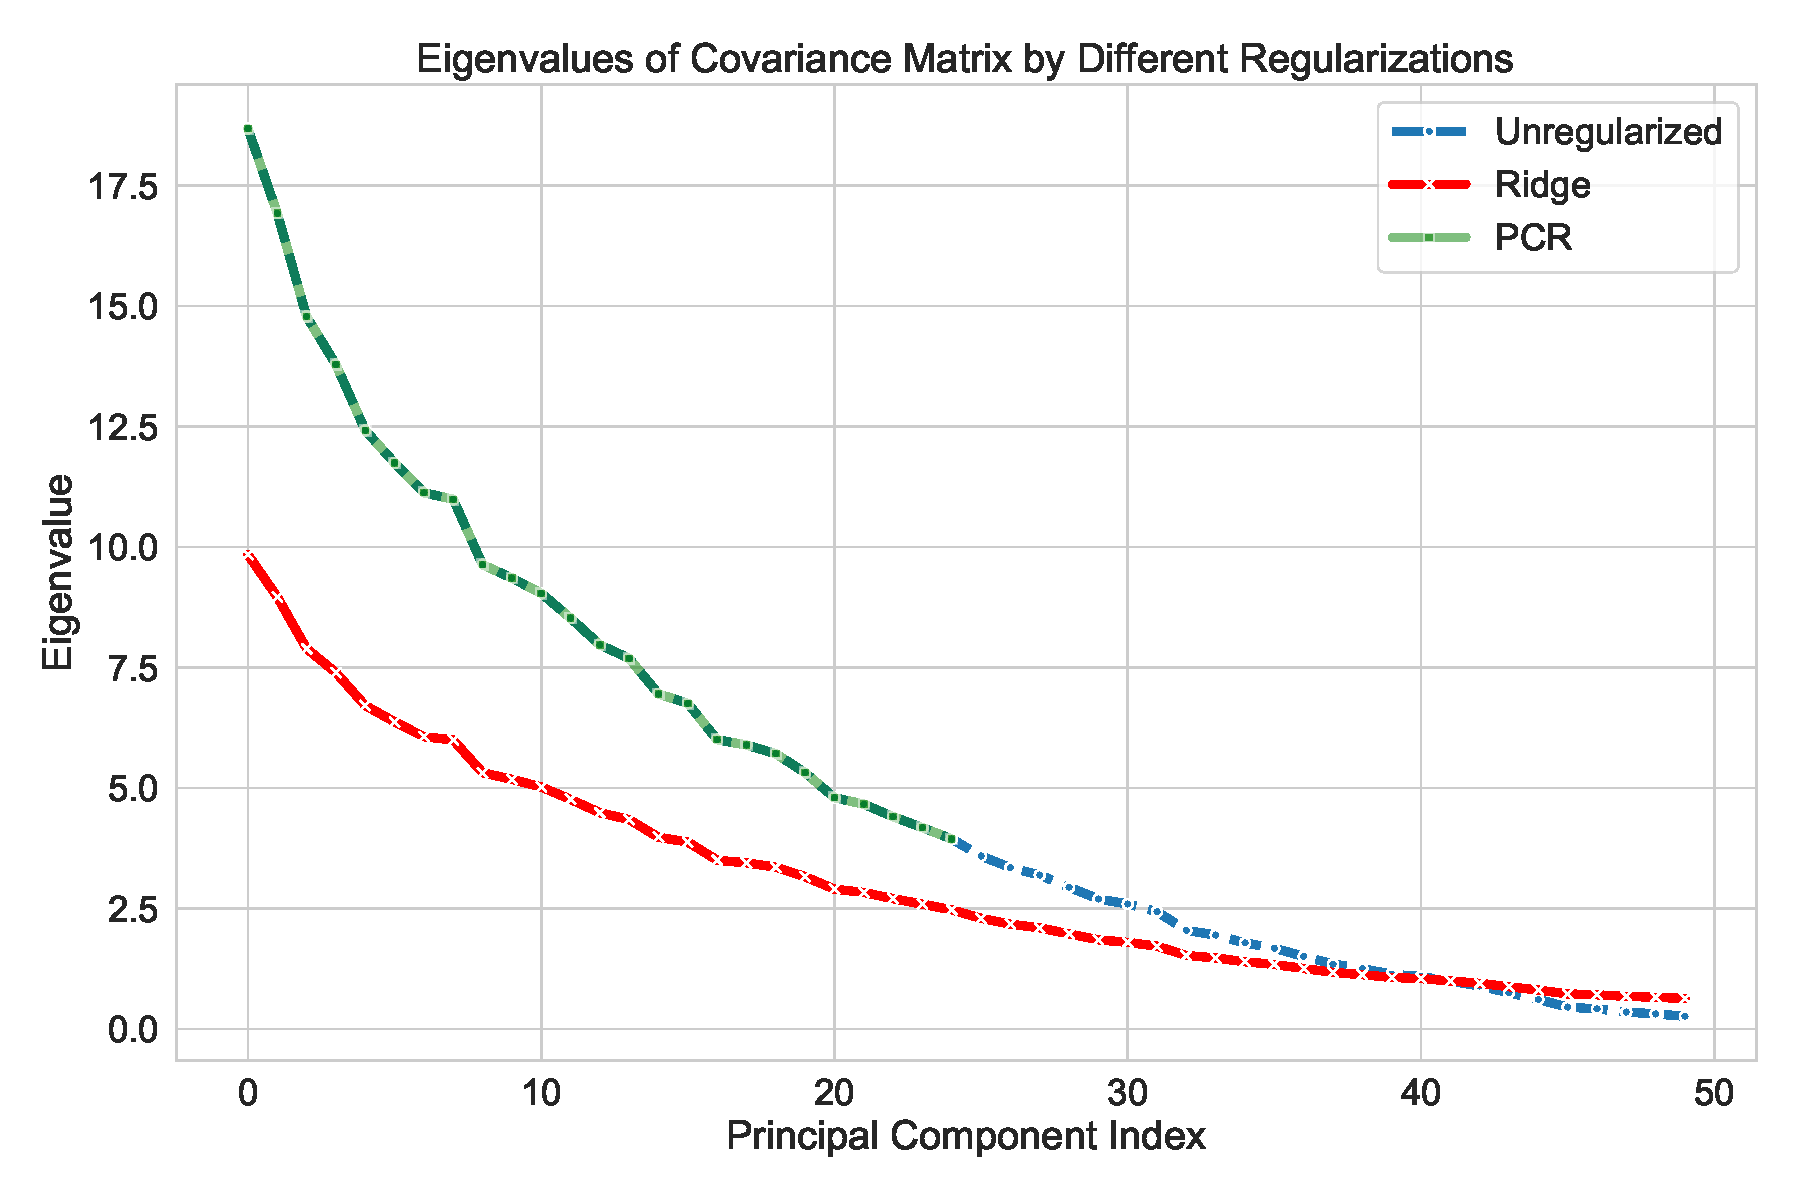
\includegraphics[width=0.8\textwidth]{figures/shrinkage/shrinkage}
    \caption{Comparison of the effect of OLS, Ridge, and PCA regularisation on the eigenvalues of the covariance matrix.}\label{fig:shrinkage}
\end{figure}

When these effective covariance matrices are inverted to form the CCA objective, these effects are reversed.
Ridge regularisation increases the magnitude of the weights associated with the largest eigenvalues and decreases the magnitude of the smallest eigenvalues.
PCA maintains the weights associated with the largest eigenvalues and sets the weights associated with the smallest eigenvalues to zero.
The visualisation underscores the intrinsic nature of each regularisation method:
\begin{itemize}
    \item \textbf{Unregularised}: Presents the unaltered spectrum, making it susceptible to noise but preserving potential subtle patterns.
    \item \textbf{Ridge}: Warps the spectrum, shrinking the largest eigenvalues and expanding the smallest eigenvalues, potentially missing subtle patterns but offering a cleaner representation of stronger associations.
    \item \textbf{PCA}: Truncates the spectrum, ignoring the smallest eigenvalues and preserving the largest eigenvalues, potentially missing subtle patterns but offering a cleaner representation of stronger associations.
\end{itemize}

However, while these shrinkage techniques can improve the performance of CCA, they do not obviously improve the interpretability of the results.
Weights are shrunk towards zero, but they are not set to zero.
This means that the model still uses all the features, and the results are not sparse.

\subsection{Sparse Regularisation}

Sparse regularisation is a powerful tool for improving the performance and interpretability of linear models.
Sparse regularisation encourages the model to use only a subset of the features, which can both help to avoid overfitting and improve the interpretability of the model.
Sparse regularisation works on the premise that only a subset of the features are relevant to the model.
Sparsity is typically achieved by adding either an L1 penalty or constraint\footnote{The L0 norm of the weight vector is the number of non-zero elements in the vector and is arguably a closer match to the goal, but the L0 norm is (a) not a proper norm in the mathematical sense and (b) not convex and so is difficult to optimize.}.
The L1 penalty is defined as:

\begin{align}
    \|u\|_1 = \sum_i |u_i|
\end{align}

Intuitively, this is the sum of the absolute values of the elements of the vector.
Now, with a foundational understanding of sparse regularisation, we review a number of approaches to adding sparsity to the CCA problem.

\paragraph{Sparse PLS: Penalised Matrix Decomposition}
Penalised Matrix Decomposition (PMD)~\citep{witten2009penalised} provides an approximate solution to the sparse CCA problem by altering the constraints of the classical CCA formulation.
Specifically, PMD replaces the constraints \(u\spsT{i} \hat{\Sigma_{ii}} u\sps{i} = 1\) with the PLS constraints \(u\spsT{i} u\sps{i}= 1\) and additionally imposes \(\|u\spsT{i}\|_1 \leq \tau\).
The optimisation problem for PMD is then given by:

\begin{align}
    & u^{opt}=\underset{u}{\mathrm{argmax}}\{ u\spsT{1} \hat{\Sigma_{12}} u\sps{2} \} \\
    & \text{subject to:} \notag \\
    & u\spsT{1} u\sps{1} = 1 , u\spsT{2} u\sps{2} = 1 \notag \\
    & \|u\sps{1}\|_1 \leq \tau_1 , \|u\sps{2}\|_1 \leq \tau_2 \notag
\end{align}

This Sparse PLS (SPLS) approximation has been highly influential as a form of Sparse CCA because it is extremely computationally efficient method \footnote{it can be solved by a variant of the power method; iteratively multiplying $u\sps{1}$ by $\hat{\Sigma_{12}}$ and soft-thresholding}.
There are a number of other sparse CCA methods that employ the PLS approximation\citep{parkhomenko2009sparse, waaijenborg2008quantifying, lindenbaum2021l0}.
However, while the PLS approximation is efficient, it means these methods inherit a bias towards the largest principal components from PLS.

To address these problems and truly tackle the sparse CCA optimisation, another class of approaches have adopted a penalised least squares approach.

\paragraph{Sparse CCA: Least Squares Approaches}

It is well known that the CCA problem can be formulated as a constrained least squares problem with the intuition that
for \(X\sps{1} u\sps{1}=1\) and \(X\sps{2} u\sps{2}=1\), correlation is maximised when the squared distance
between \(X\sps{1} u\sps{1}\) and \(X\sps{2} u\sps{2}\) is minimised. \citep{golub1995canonical} proved the
convergence of a simple algorithm which alternates between solving the least squares problem for \(u\sps{1}\) and
\(u\sps{2}\) while keeping the other fixed.

With this intuition, \cite{wilms2015sparse} and \cite{mai2019iterative} separately proposed iterative penalised least
squares methods for sparse CCA\@.

\begin{align}
    \label{eq:mai}
    u^{opt} &= \underset{u}{\mathrm{argmin}} \left\{ \|X\sps{1}u\sps{1} - X\sps{2}u\sps{2}\|_2^2 + P(u) \right\} \\
    &\text{subject to:} \notag \\
    &u\spsT{1} \hat{\Sigma_{11}} u\sps{1}=1 \notag \\
    &u\spsT{2} \hat{\Sigma_{22}} u\sps{2}=1 \notag
\end{align}

Where \(P(u)\) is a penalty function.
The penalty term can be any function that penalizes the norm of the vector \(u\).
\citep{mai2019iterative} proved that solving the subproblems where one of $u\sps{i}$ is fixed is easy for one-homogenous $P$ where
\( P((\mu + 1)\theta) = (\mu + 1)P(\theta) \) which notably includes the lasso penalty.
This means a sparse CCA based
on alternating lasso regressions can be solved relatively efficiently using existing solvers.
However, the one homogenous penalty in practice limits the flexibility of the method.
For example, the elastic net penalty is not one-homogenous and therefore cannot be used with this method.
\citet{6556581} and \cite{Mullins2021} added ridge penalties to the subproblems to improve the conditioning of the problem in a way that could be considered a form of elastic net regularisation but the subproblems no longer correctly optimize the global objective\footnote{when rescaling the penalised solutions back to unit variance}.

\paragraph{Sparse CCA: Proximal Gradient Descent and ADMM}
\citet{kanatsoulis2018structured} proposed solving equation~\ref{eq:mai} for more general classes of $P$ using the alternating direction method of multipliers (ADMM)~\citep{boyd2011distributed}.
\cite{fu2017scalable} propose a regularised CCA based on an alternative classical CCA formulation, sometimes called the MAXVAR formulation, which views the problem as a constrained least squares with an auxiliary representation $T$\citep{carroll1968generalisation,kettenring1971canonical}.

\begin{align}
    \label{eq:fu}
    \underset{U, T}{\mathrm{argmin}}\left\{\sum_i \|X\sps{i} U\sps{i} - T\|_F^2\right\}\\
    \text{subject to: }T^\top T = I\\
\end{align}

In this formulation, \(U\sps{i}\) represents the \gls{weights} for the $i^{\text{th}}$ view, and \(T\) denotes the latent variable matrix.
The premise is that when \(T\) closely mirrors \(X\sps{i} U\sps{i}\) across all \(i\), the scores correlate.
Notably, this method is adaptable to multiple views.
The authors employed proximal gradient descent for regularisation, specifically suited for penalties like the lasso.
While these methods are flexible, they don't have the plug-and-play nature of the penalised least squares methods.
Not just a matter of convenience, this means that these methods are not compatible with existing solvers for regularised least squares problems like for example total variation regularisation solvers in nilearn, which are often highly optimised for specific problems and modalities.

\paragraph{Structured Regularisation}

As highly structured data, linear models using both Structural and Functional \acrshort{mri} data have been shown to benefit from structured regularisation methods but notably these methods have not been applied to CCA.
Total variation regularisation, which biases spatially neighboring weights to be similar, has been shown to improve the performance of PCA \citep{de2017structured} and regression \citep{michel2011total,dohmatob2014benchmarking, baldassarre2012structured}.
Similarly, Laplacian (or \textit{GraphNet}) regularisation, which induces a similar spatial bias with additional smoothness, has been shown to improve the performance of CCA on functional MRI data \citep{grosenick2013interpretable}.

Having discussed the benefits of both shrinkage (e.g., PCA-CCA, Ridge CCA, PLS), sparsity (SPLS, Sparse CCA), and structure (Total Variation, Laplacian) in handling high-dimensional, noisy, and structured data, a natural progression is to integrate these advantages.
Specifically, the challenge lies in creating a framework that allows for users to match the regularisation method to their data and research question, enhancing the interpretability and performance of Brain-Behaviour association models.
The solution?
A method that employs readily available regularised regression solvers, allowing for flexible and tunable regularisation in CCA.
This leads us to propose the Flexible Regularised Alternating Least Squares (FRALS).

\section{Methods - Flexible Regularised Alternating Least Squares (FRALS)}\label{subsec:flexible-regularised-alternating-least-squares-(frals)}

The primary goal of our Flexible Regularised Alternating Least Squares framework is to provide a versatile and user-friendly interface for Canonical Correlation Analysis (CCA). This is achieved by designing the framework to be compatible with any scikit-learn compatible regularised least squares solver. This compatibility is pivotal as it allows researchers and practitioners to leverage the extensive range of solvers available in scikit-learn, a popular machine learning library in Python.

This approach marks a significant departure from traditional methodologies in CCA, which often focused on developing or utilizing specific solvers tailored for particular types of data or computational constraints.
By contrast, \acrshort{frals} democratizes access to advanced CCA techniques, allowing users to select solvers that best fit their specific data characteristics, computational needs, or familiarity.
Such flexibility is particularly advantageous in interdisciplinary fields like neuroimaging, where diverse datasets and varying levels of technical expertise are common.

For example, users dealing with high-dimensional, sparse neuroimaging data could opt for solvers optimised for such datasets, while those needing parallel computation for large data sets might choose solvers with GPU acceleration capabilities.
In principle, \acrshort{frals} can even be used with Neural Network-based solvers, which are becoming increasingly popular in machine learning\footnote{Though for reasons that will later become clear, we do not reccommend this!}.
This adaptability enhances \acrshort{frals}' accessibility and future-proofs the framework against evolving computational technologies and data analysis needs.

In the \acrshort{frals} framework, we consider the formulation for a single latent variable \(t\) with regularisation \(\lambda_i P_i\) on the weights \(u^{(i)}\):

\begin{align}
    \underset{u}{\mathrm{argmin}}\left\{\sum_i \|X^{(i)} u^{(i)} - t\|_2^2 + \textcolor{red}{\lambda_i P_i(u^{(i)})} \right\}\\
    \text{subject to: }t^\top t = 1 \notag
\end{align}

This problem can be decomposed into three subproblems.
The first subproblem for the auxiliary variable \(t\):

\begin{align}
    \underset{t}{\mathrm{argmin}}\left\{\sum_i \|X^{(i)} u^{(i)} - t\|_2^2\right\}\\
    \text{subject to: }t^\top t = 1 \notag
\end{align}

is a standard least squares problem and can be solved in closed form by averaging \(X^{(i)} u^{(i)}\) and normalizing i.e. \(t = \frac{\sum_i X^{(i)} u^{(i)}}{\|\sum_i X^{(i)} u^{(i)}\|_2}\).
As shown earlier this makes \(t\) an estimate of the latent variables of a generative CCA model.

The subproblems for the weights \(u^{(i)}\):

\begin{align}
    \underset{u^{(i)}}{\mathrm{argmin}}\left\{\|X^{(i)} u^{(i)} - t\|_2^2 + \textcolor{red}{\lambda_i P_i(u^{(i)})} \right\}
\end{align}

are regularised least squares problems that can be solved using any suitable regularised least squares solver\footnote{We could also in principle replace $X^{(i)} u^{(i)}$ with $f(X^{(i)})$ for any function $f$ including kernels, neural networks, or random forests}.

In this chapter, we illustrate the power of the \acrshort{frals} framework by implementing the well-tested Elastic Net solver from the \texttt{scikit-learn} package~\citep{pedregosa2011scikit}, where \(P_i = \alpha_i \times \text{l1\_ratio} \|u^{(i)}\|_1 + \alpha_i \times (1-\text{l1\_ratio}) \|u^{(i)}\|_2^2\), allowing for independent tuning of shrinkage and sparsity of the weights in both views.

In summary, the \acrshort{frals} framework is a flexible and user-friendly interface for CCA that allows users to combine scikit-learn compatible regularised least squares solvers to solve regularised CCA problems.


\section{Experiments}

In this section, we outline the methodologies employed in our study of \acrshort{frals} and related techniques.

\subsection{Datasets}\label{subsec:datasets}

For this chapter, we chose the \acrshort{hcp} and the \acrshort{adni} datasets to facilitate comparison with two influential brain-behaviour studies \citep{smith2015positive, monteiro2016multiple} as well as the tutorial paper that this chapter is loosely related to \citep{mihalik2022canonical}.
We are particularly interested in the performance of an Elastic Net \acrshort{frals}  on these datasets as Ridge CCA has been shown to outperform PLS \citep{mihalik2022canonical}, implying that shrinkage regularisation is beneficial, and Sparse PLS has been shown to outperform PLS\cite{monteiro2016multiple}, implying that sparsity is beneficial.
We therefore expect that Elastic Net \acrshort{frals} will outperform PLS, Ridge CCA, and Sparse PLS on these datasets.

\subsubsection{The Human Connectome Project (\acrshort{hcp})}

The \acrshort{hcp} offers publicly available resting-state functional MRI (rs-fMRI) and non-imaging measures like demographics, psychometrics, and other behavioral measures.
Specifically, we sourced data from 1003 subjects out of the 1200-subject data release of the \acrshort{hcp}.
The rs-fMRI data provided brain connectivity matrices. These were derived from pairwise partial correlations between subject components obtained through group independent component analysis (ICA), utilizing 25 components. This resulted in 300 brain variables, corresponding to the lower triangle of the connectivity matrix. In our analysis, 145 non-imaging subject measures were incorporated, similar to prior studies, with the exception of 13 measures (ASR\_Aggr\_Pct, ASR\_Attn\_Pct, ASR\_Intr\_Pct, ASR\_Rule\_Pct, ASR\_Soma\_Pct, ASR\_Thot\_Pct, ASR\_Witd\_Pct, DSM\_Adh\_Pct, DSM\_Antis\_Pct, DSM\_Anxi\_Pct, DSM\_Avoid\_Pct, DSM\_Depr\_Pct, DSM\_Somp\_Pct) that were unavailable in the 1200-subject data release. Furthermore, nine confounding variables, including the acquisition reconstruction software version, a summary statistic of head motion during rs-fMRI acquisition, weight, height, systolic and diastolic blood pressure, hemoglobin A1C level, and cube-root of total brain and intracranial volumes as estimated by FreeSurfer, were regressed out from both data types.
More details can be found in \citet{smith2015positive, mihalik2022canonical}.
We summarize the parameters of the \acrshort{hcp} data in table~\ref{tab:hcp-parameters}.

\begin{table}
    \centering
    \caption{HCP Data Parameters}
    \begin{tabular}{| l | l |}
        \hline
        \textbf{Parameter}                        & \textbf{Value} \\
        \hline
        Number of samples (\textit{n})            & 1003           \\
        Number of features in View 1 (\textit{p}) & 19900          \\
        Number of features in View 2 (\textit{q}) & 145            \\
        \hline
    \end{tabular}\label{tab:hcp-parameters}
\end{table}

\subsubsection{The Alzheimer's Disease Neuroimaging Initiative (ADNI)}

Accessible at \url{adni.loni.usc.edu}, the \acrshort{adni} database was initiated in 2003. 
Its primary aim is the examination of how well serial MRI, PET (Positron Emission Tomography), biological markers, along with clinical and neuropsychological assessments, track the progression of Mild Cognitive Impairment (MCI) and the early stages of Alzheimer’s disease. 
In our study, we utilised data from a subset of 592 unique individuals, comprising 309 males (average age 74.68 ± 7.36 SEM) and 283 females (average age 72.18 ± 7.50 SEM). This subset included 147 healthy controls, 335 individuals with Mild Cognitive Impairment (MCI), and 110 diagnosed with dementia. 
T1 weighted structural MRI (sMRI) scans were the source of whole-brain voxel-based grey matter volumes. The sMRI data underwent preprocessing with SPM12\citep{ashburner2014spm12}, which involved segmentation, normalisation using DARTEL, reslicing to a resolution of \(2 \times 2 \times 2 \, \text{mm}^3\)
, and spatial smoothing using a Gaussian kernel with 2 mm full width at half maximum (FWHM). A grey matter voxel selection mask, with a threshold of $\geq$10\%, was applied to all participants' scans, resulting in 168,130 brain variables. 
The Mini-Mental State Examination (MMSE) is a widely recognised neurocognitive test comprising 30 questions across five cognitive domains: orientation (questions 1-10), registration (questions 11-13), attention and calculation (questions 14-18), recall (questions 19-21), and language (questions 22-30)\citep{folstein1975mini}. 
An additional item was included in our study to account for the number of attempts a subject needed to correctly respond to the registration domain questions, leading to a total of 31 variables. As in \citet{monteiro2016multiple}, no confounds were removed from these data.
We summarize the parameters of the \acrshort{adni} data in table~\ref{tab:adni-parameters}.

\begin{table}
    \centering
    \caption{ADNI Data Parameters}
    \begin{tabular}{| l | l |}
        \hline
        \textbf{Parameter}                        & \textbf{Value} \\
        \hline
        Number of samples (\textit{n})            & 592            \\
        Number of features in View 1 (\textit{p}) & 168130         \\
        Number of features in View 2 (\textit{q}) & 31             \\
        \hline
    \end{tabular}\label{tab:adni-parameters}
\end{table}

\subsection{The predictive framework for CCA}\label{subsec:the-predictive-framework-for-cca}

To evaluate the performance of CCA models, we employ a standard predictive framework.
We split the data into training and test sets using a 80:20 split, and use the training set to fit the model.
We then use the test set to evaluate the model's performance.
Where relevant, pre-processing is performed on the training set and the same pre-processing is applied to the test set.
This is important to avoid data leakage, where information from the test set is used to fit the model.

\subsubsection{Model Comparisons}
In the experiments in this section, we are interested in illustrating the effects of tunable shrinkage and sparsity on the performance and interpretability of CCA models, enabled by the \acrshort{frals} framework.
To this end, we compare the performance of Elastic Net \acrshort{frals} with other CCA variants, including PCA, PLS, Ridge CCA, Sparse PLS, and Elastic Net CCA\@.

\begin{table}[h]
    \centering
    \caption{Employed CCA Variants}
    \begin{tabular}{|l|l|l|l|}
        \hline
        \textbf{Model}               & \textbf{Abbreviation} & \textbf{Hyperparameters}                         & \textbf{Hyperparameter Range}                                                                                             \\
        \hline
        Principal Component Analysis & PCA                   & -                                                & -                                                                                                                         \\
        \hline
        Regularised CCA              & RCCA                  & \(c_1, c_2\)                                     & 0-1 (log scaled)                                                                                                          \\
        \hline
        FRALS - Elastic              & Elastic               & \(\alpha_1, \alpha_2, \text{l1}_1, \text{l1}_2\) & (1e-5,1e-1), (0-1)                                                                                                        \\
        \hline
        Partial Least Squares        & PLS                   & -                                                & -                                                                                                                         \\
        \hline
        Sparse PLS                   & SPLS                  & \(\tau_1, \tau_2\)                               & 0-1\footnote{As in \citet{witten2013package}, these are converted to 0-$\sqrt {\text{number of features}}$)} (log scaled) \\
        \hline
    \end{tabular}\label{table:cca-variants}
\end{table}

\subsubsection{Model Selection}

For the models that require hyperparameter tuning, we use a grid search to find the best hyperparameters.
Specifically, we use 5-fold cross-validation to evaluate the performance of a model with a given set of hyperparameters on 5 different splits of the training data with non-overlapping validation sets.
We optimise for the hyperparameters that give the best average out of sample correlation.


\section{Results}

\subsection{\acrshort{hcp} Results}

Next, we consider the results of applying the various CCA variants to the \acrshort{hcp} data.
Since the \acrshort{hcp} data is high-dimensional, we drop CCA from the analysis since it would produce random results.

\subsubsection{Out of Sample Correlation}

Both Ridge CCA and Elastic Net outperformed PLS and SPLS in terms of holdout correlation captured (Figure~\ref{fig:performance}).
This suggests that tunable L2 regularisation is important, even for very high-dimensional data, and that resorting to PLS is suboptimal.
On the other hand, while the additional sparsity improved SPLS over PLS (consistent with previous work \cite{monteiro2016multiple}), it did not improve the performance of the Elastic Net model over Ridge CCA\@.

\begin{figure}[h]
    \centering
    \includegraphics[width=0.5\linewidth]{figures/hcp/holdout_correlations}
    \caption{\textbf{HCP:} Out-of-sample canonical correlations for each model.}
\end{figure}

Nonetheless, the Elastic Net model did produce sparser weights than the Ridge CCA model (Figure~\ref{fig:sparsity}) with the Elastic Net model using 241 and 96 non-zero weights for the brain and behaviour views respectively.
This is compared to 300 and 145 non-zero weights for the brain and behaviour views respectively for the Ridge CCA model.
The SPLS model used even fewer variables with 118 and 56 non-zero weights for the brain and behaviour views respectively.
Given that the Elastic Net model can produce the same performance as the Ridge CCA model with fewer variables, we might then be inclined to prefer the Elastic Net model.

\begin{table}[h]
    \centering
    \caption{\textbf{HCP:} Number of non-zero \gls{weights} for each model.}
    \begin{tabular}{|c|c|c|}
        \hline
        Model       & Brain Weights & Behaviour Weights \\
        \hline
        PCA         & 300           & 145               \\
        RCCA        & 300           & 145               \\
        Elastic Net & 241           & 96                \\
        PLS         & 300           & 145               \\
        SPLS        & 118           & 56                \\
        \hline
    \end{tabular}\label{tab:brain-behaviour-weights-hcp}
\end{table}

\subsubsection{Behaviour Weights}

Figure\ref{fig:behaviour} plots the top 8 positive and negative non-imaging \gls{weights} for each model.
This is to illustrate some of the effects we have observed in the previous section.
PCA finds a mode of variation in the behavioural data that is positively correlated with psychiatric and life function tests and negatively correlated with a number of emotion and personality tests.
The RCCA and Elastic Net models find a mode of variation in the behavioural data that is negatively correlated with the Line Orientation test and to a lesser extent smoking and positively correlated with a number of other cognitive tests.
The PLS model finds a mode of variation in the behavioural data that is somewhat similar to the `positive-negative' mode in \citet{smith2015positive} with a positive correlation with agreeableness, vocabulary tests, and feelings about ones' life and a strong negative correlation with smoking, rule-breaking, and antisocial personality traits.
The SPLS mode is similar but selects out the rule-breaking and antisocial personality traits in favour of the vocabulary tests and smoking. This appears consistent with the additional preprocessing steps in \citet{smith2015positive}, which included a top-100 PCA projection of both the brain and behaviour data.

\begin{figure}[h]
    \centering
    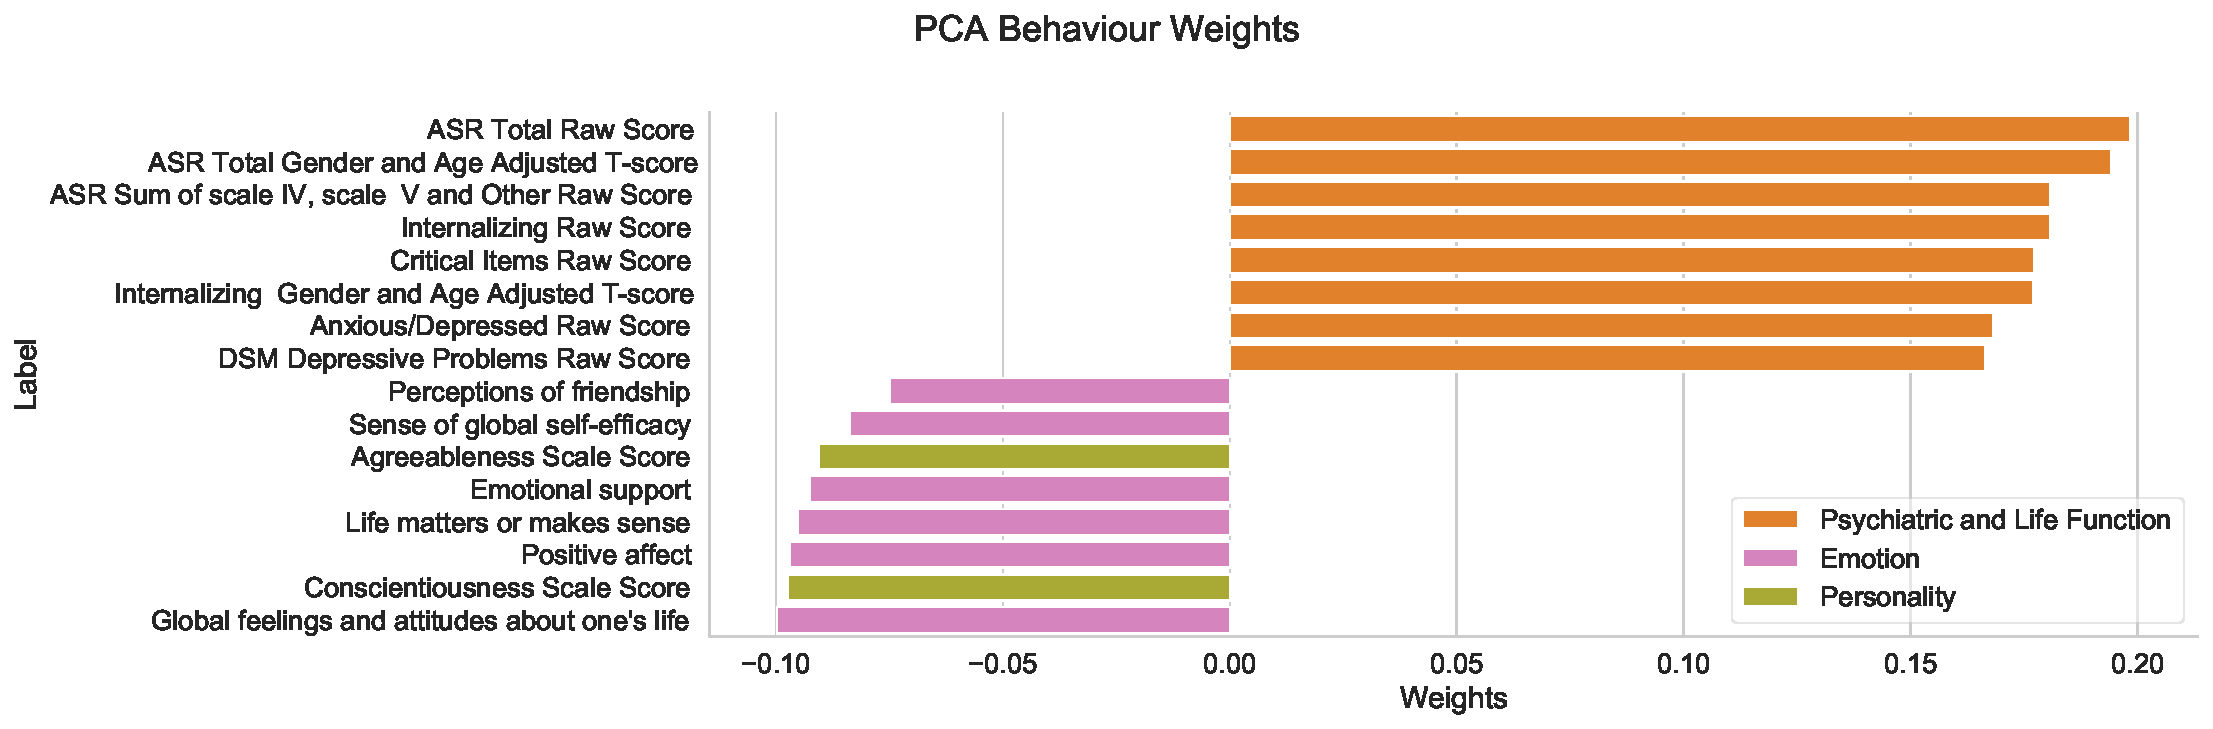
\includegraphics[width=0.8\linewidth]{figures/hcp/PCA behaviour weights}
    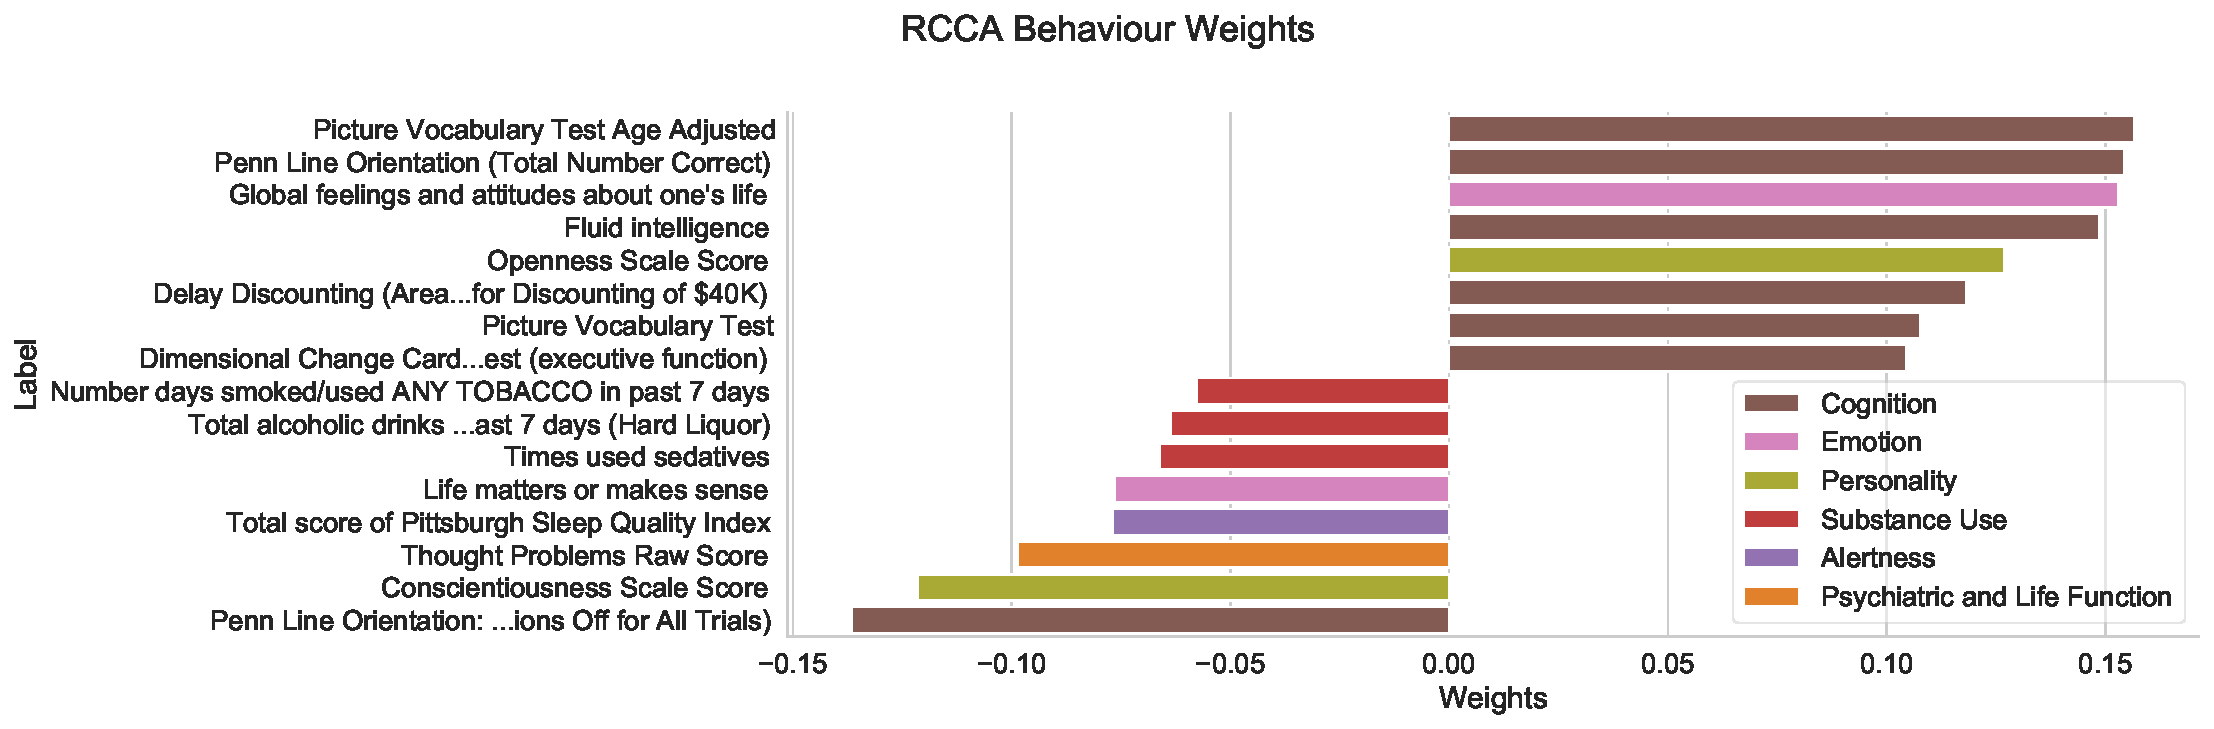
\includegraphics[width=0.8\linewidth]{figures/hcp/RCCA behaviour weights}
    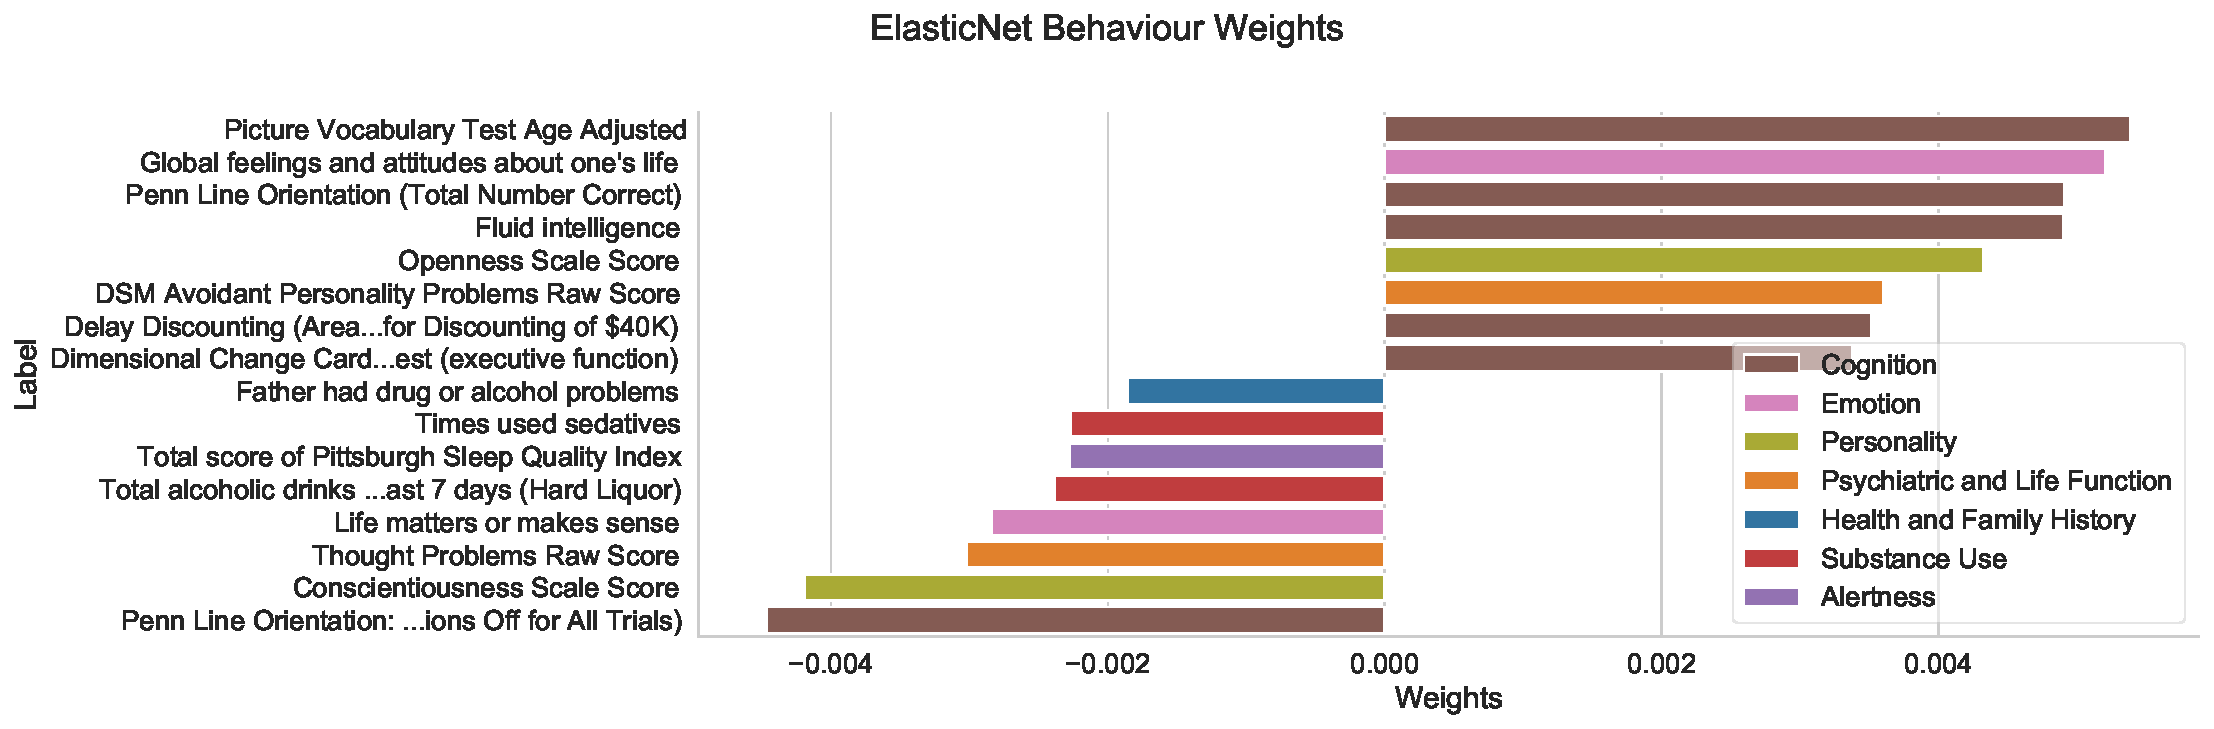
\includegraphics[width=0.8\linewidth]{figures/hcp/ElasticNet behaviour weights}
    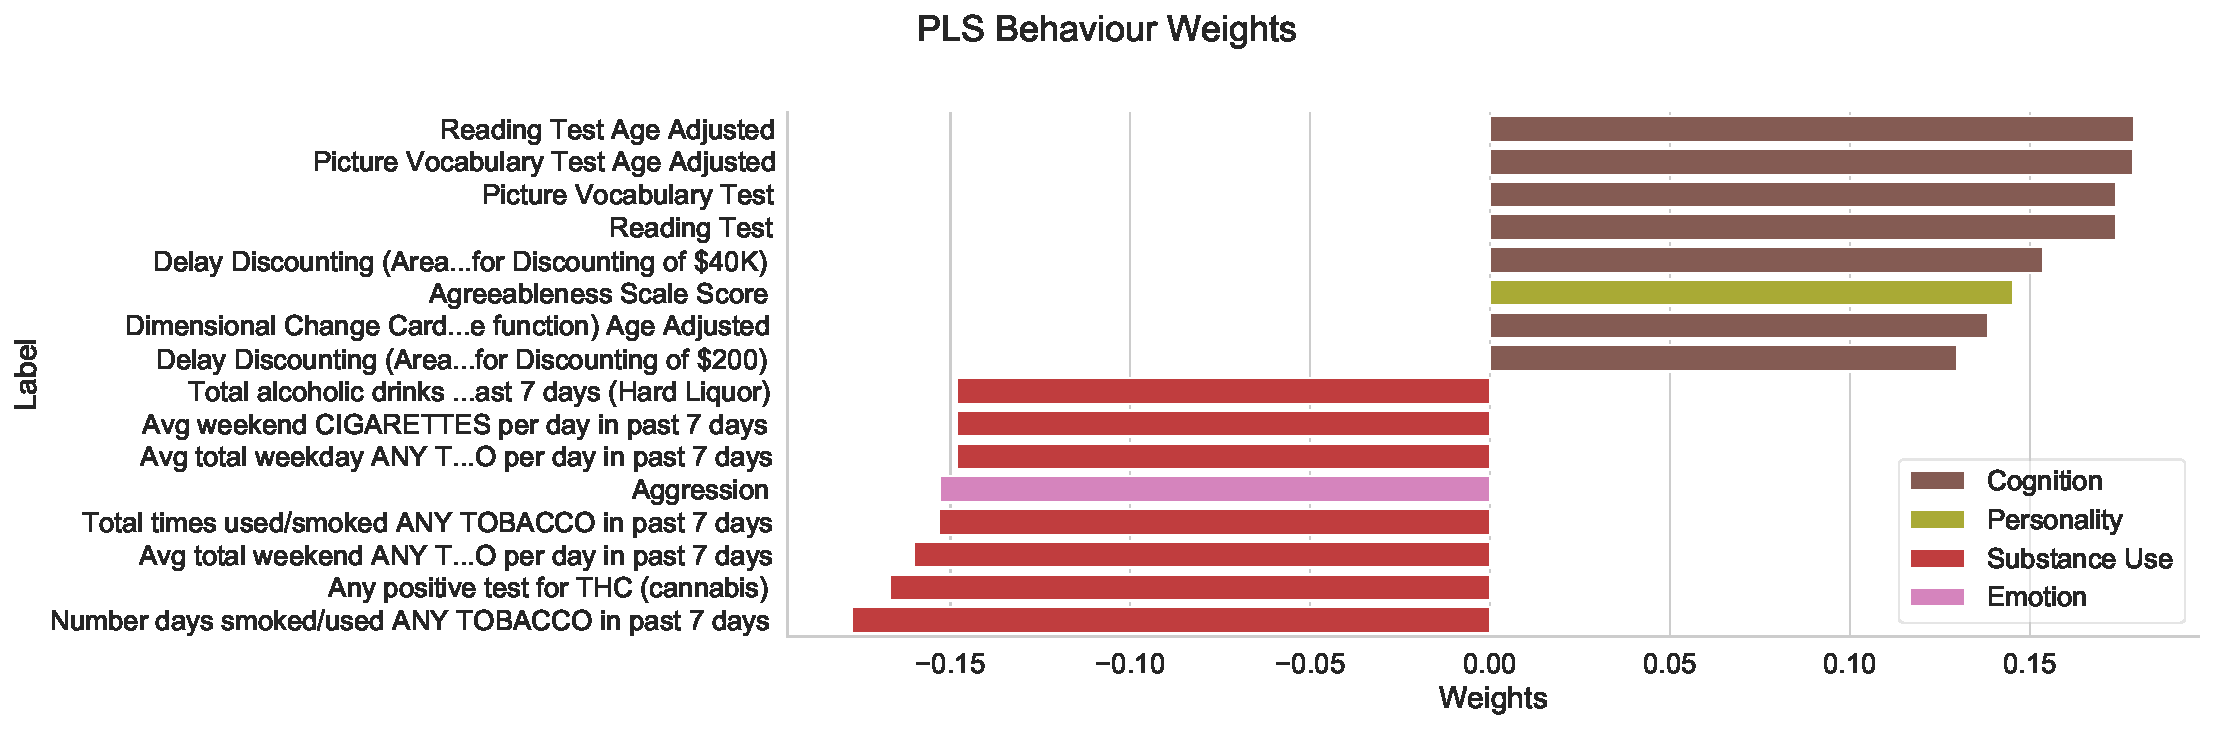
\includegraphics[width=0.8\linewidth]{figures/hcp/PLS behaviour weights}
    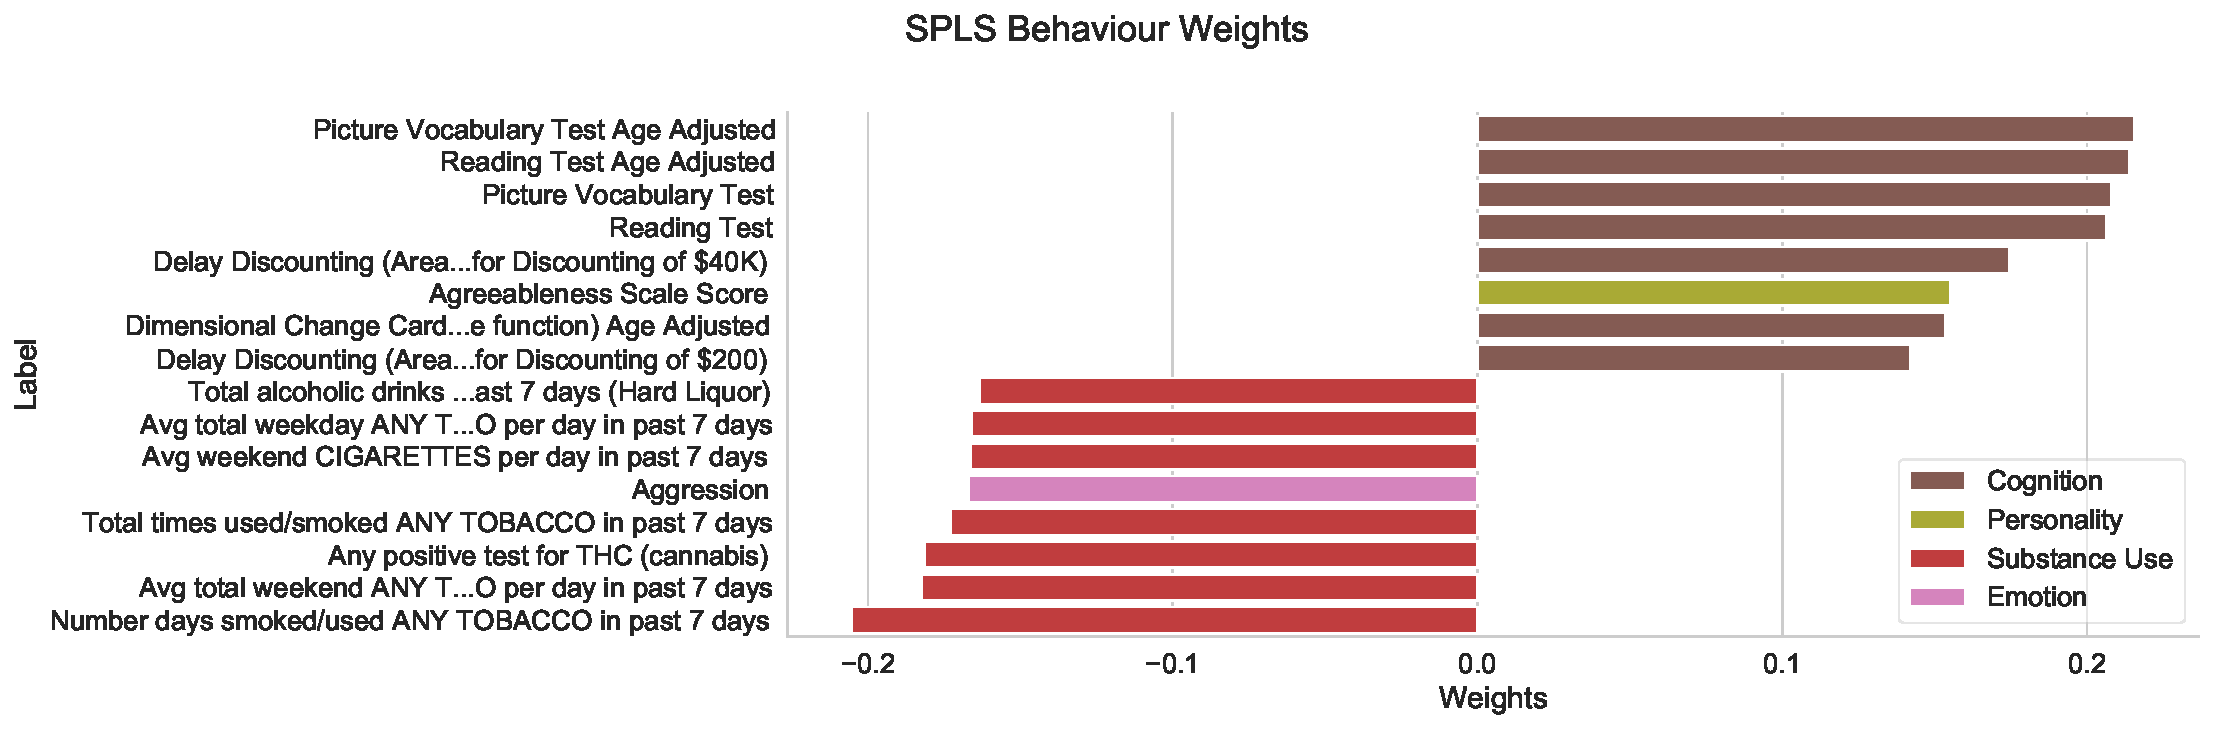
\includegraphics[width=0.8\linewidth]{figures/hcp/SPLS behaviour weights}
    \caption{\textbf{HCP:} Top 8 positive and negative non-imaging \gls{weights} for each model}\label{fig:behaviour}
\end{figure}

\subsubsection{Brain Connectivity Weights}

In this section, we use two different methods to visualize the brain connectivity weights.
The first method is to use chord diagrams to visualize the top 8 positive and negative brain \gls{weights} for each model.
This approach is inspired by the chord diagrams used in \cite{smith2015positive}.
The second method is to use surface maps to visualize the brain connectivity weights.
This approach has been used by both \cite{ferreira2022hierarchical} and \cite{smith2015positive}.

\paragraph{Chord Diagrams}
We grouped the nodes of the connectivity matrix of our data into 7 parcels according to the Yeo 7 network parcellation \cite{yeo2011organisation}.
This was achieved by assigning each node to the network with the highest voxelwise overlap.
These are then arranged around the circumference of the chord diagram using the Nichord package\citep{bogdan2023connsearch}.
The plots then show the 8 strongest positive and negative \gls{weights} for each model as `chords'.
The chord diagrams in Figure~\ref{fig:chord_weights} show the top 8 positive and negative brain \gls{weights} for each model.

\begin{itemize}
    \item The \textbf{RCCA} model displays a diverse set of connections across all networks, with especially prominent weights in the \textcolor{red}{somatomotor} and \textcolor{blue}{default mode} networks.

    \item The \textbf{ElasticNet} model presents similar connections between the \textcolor{red}{somatomotor} and \textcolor{blue}{default mode} networks.

    \item The \textbf{PLS} model exhibits strong connections between the \textcolor{green}{frontoparietal} and \textcolor{pink}{visual} networks.

    \item The \textbf{SPLS} model exhibits similar connections between the \textcolor{green}{frontoparietal} and \textcolor{pink}{visual} networks.
\end{itemize}

This is perhaps consistent with the behaviour data as the somatomotor network is associated with motor function and sensory processing which is related to the Line Orientation test, requiring spatial reasoning and motor coordination.

The correlations made by the PLS and SPLS models between substance abuse and cognitive tests could be due to the significant role the frontoparietal network plays in executive function, which can be impaired by substance abuse.
Likewise, the visual network is likely involved in a number of the cognitive tests and could be disrupted by substance abuse.

The RCCA and ElasticNet models might be detecting more integrative and possibly more developed cognitive functions, while the PLS and SPLS models might be highlighting the more immediate cognitive processes that can be disrupted by substance abuse.

\begin{figure}[h]
    \centering
    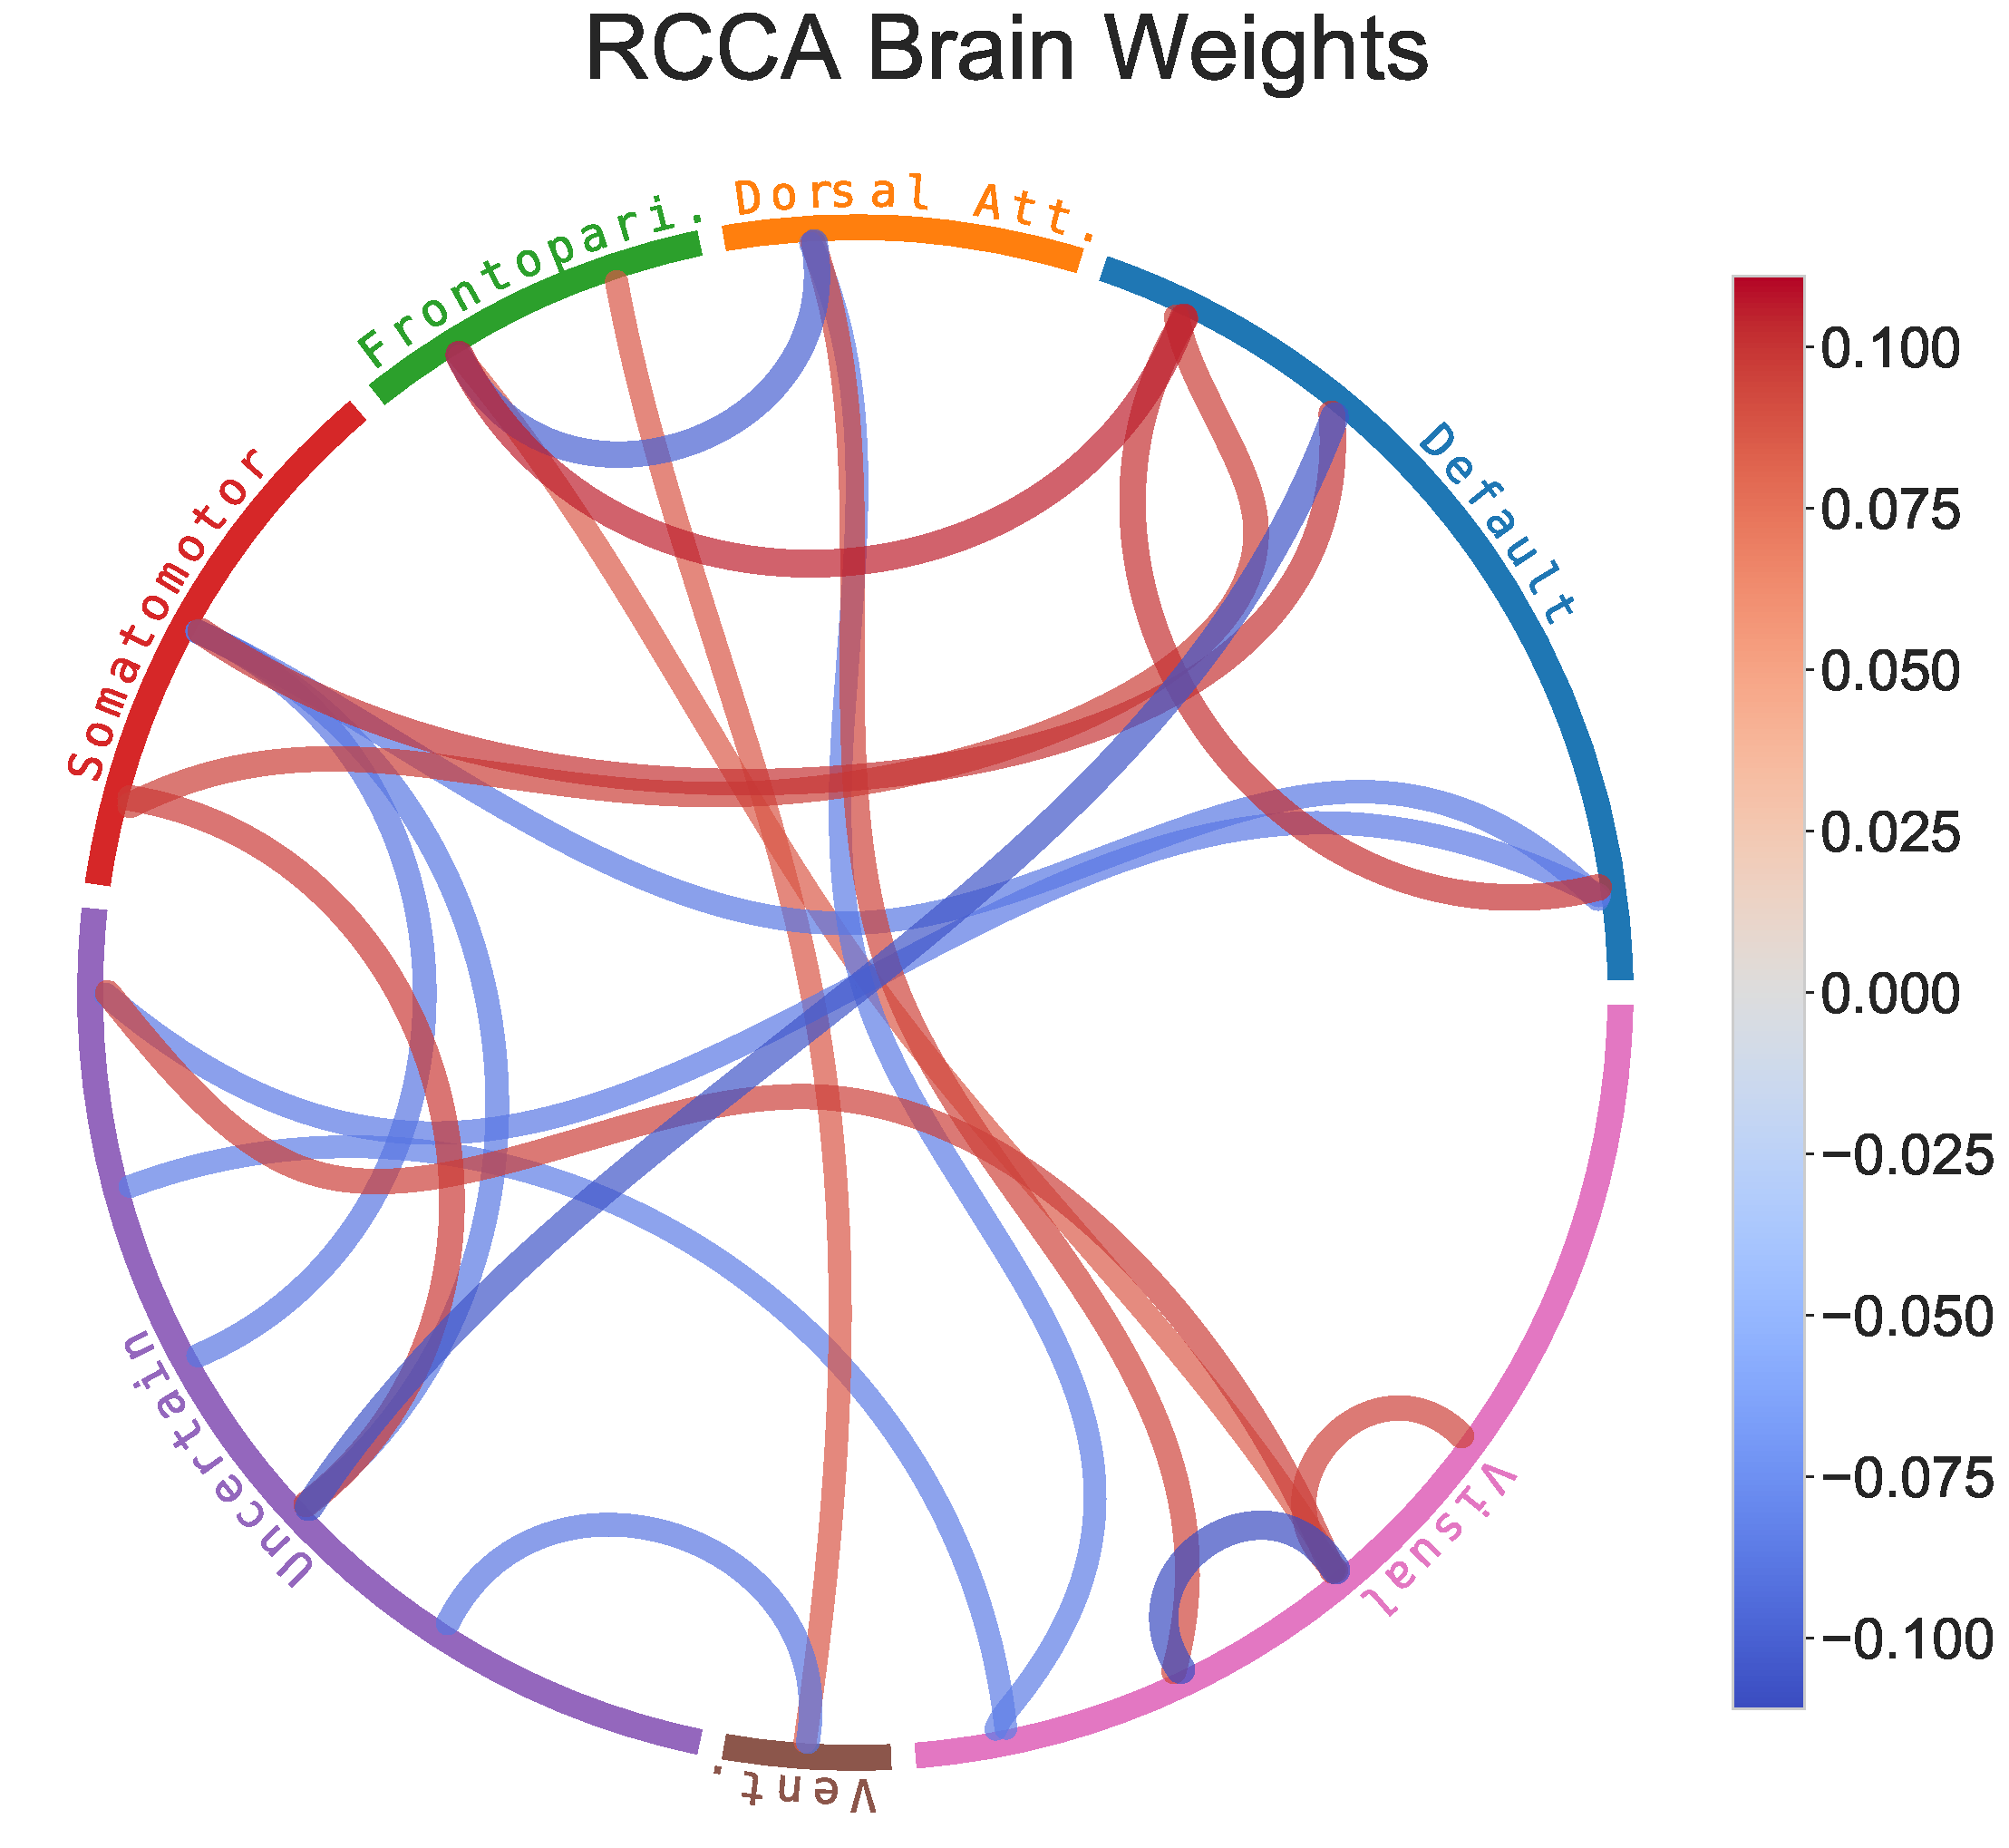
\includegraphics[width=0.49\linewidth]{figures/hcp/RCCA brain weights}
    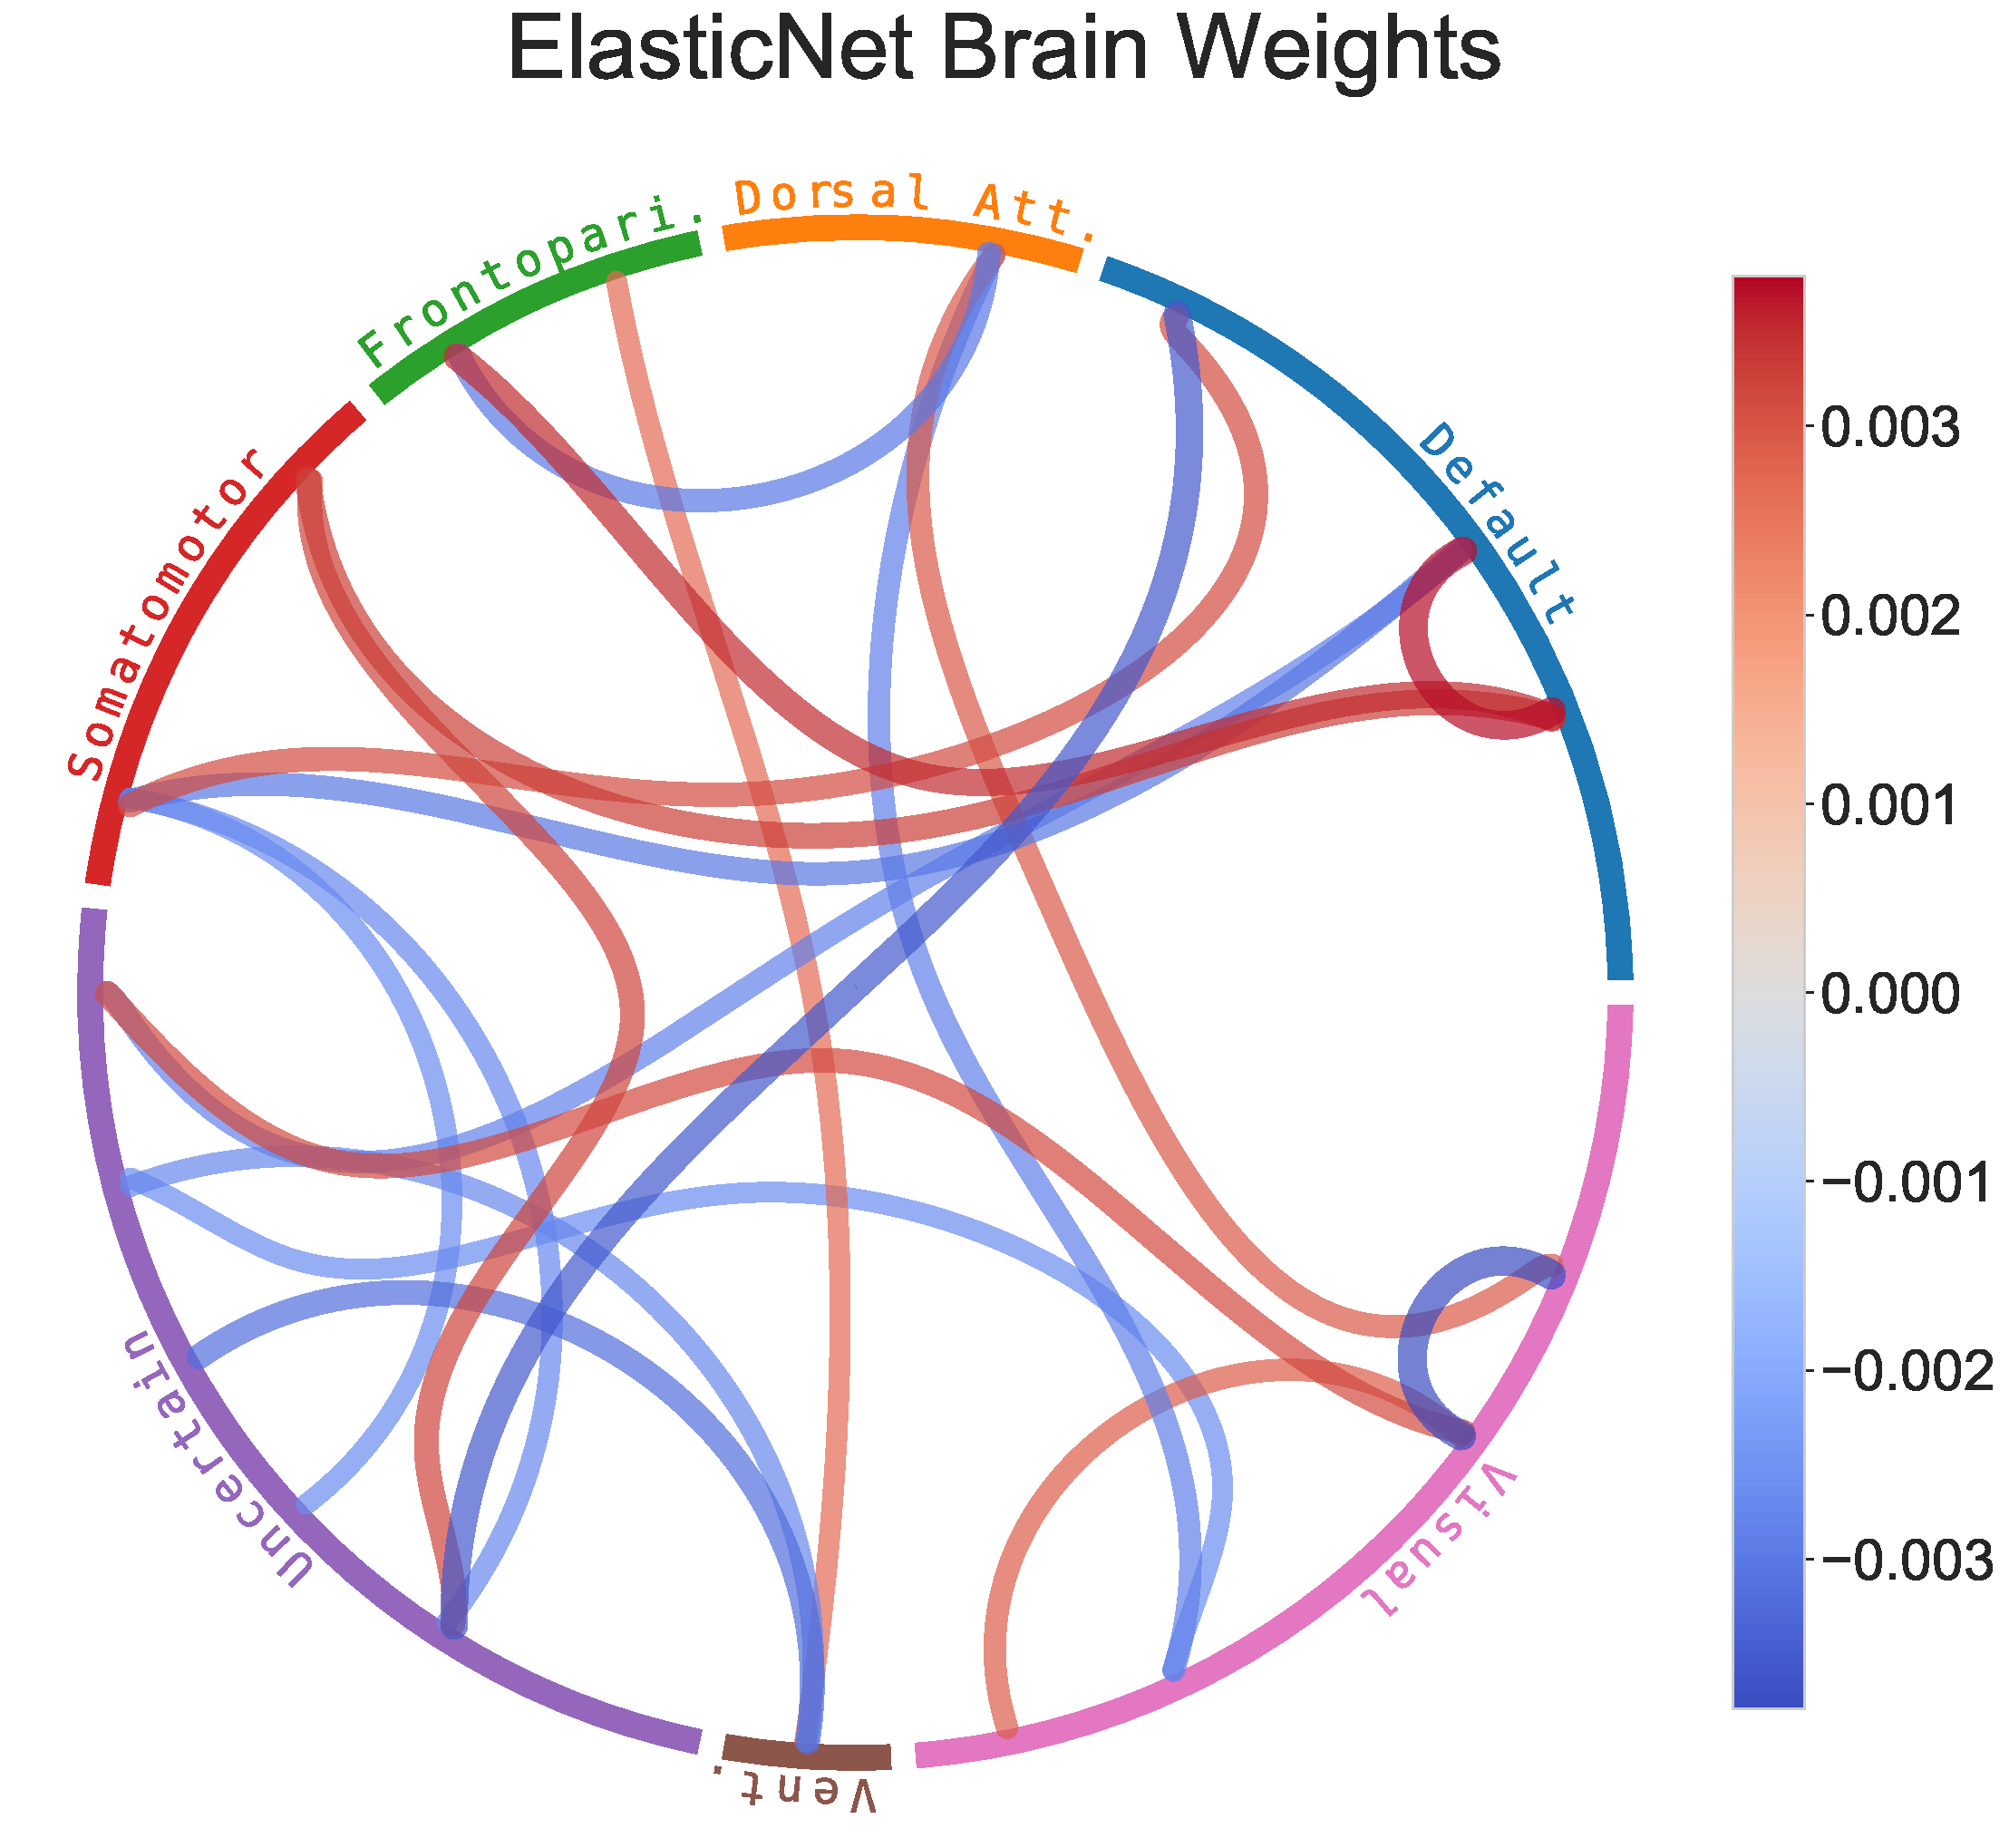
\includegraphics[width=0.49\linewidth]{figures/hcp/ElasticNet brain weights}
    \includegraphics[width=0.49\linewidth]{figures/hcp/PLS brain weights}
    \includegraphics[width=0.49\linewidth]{figures/hcp/SPLS brain weights}
    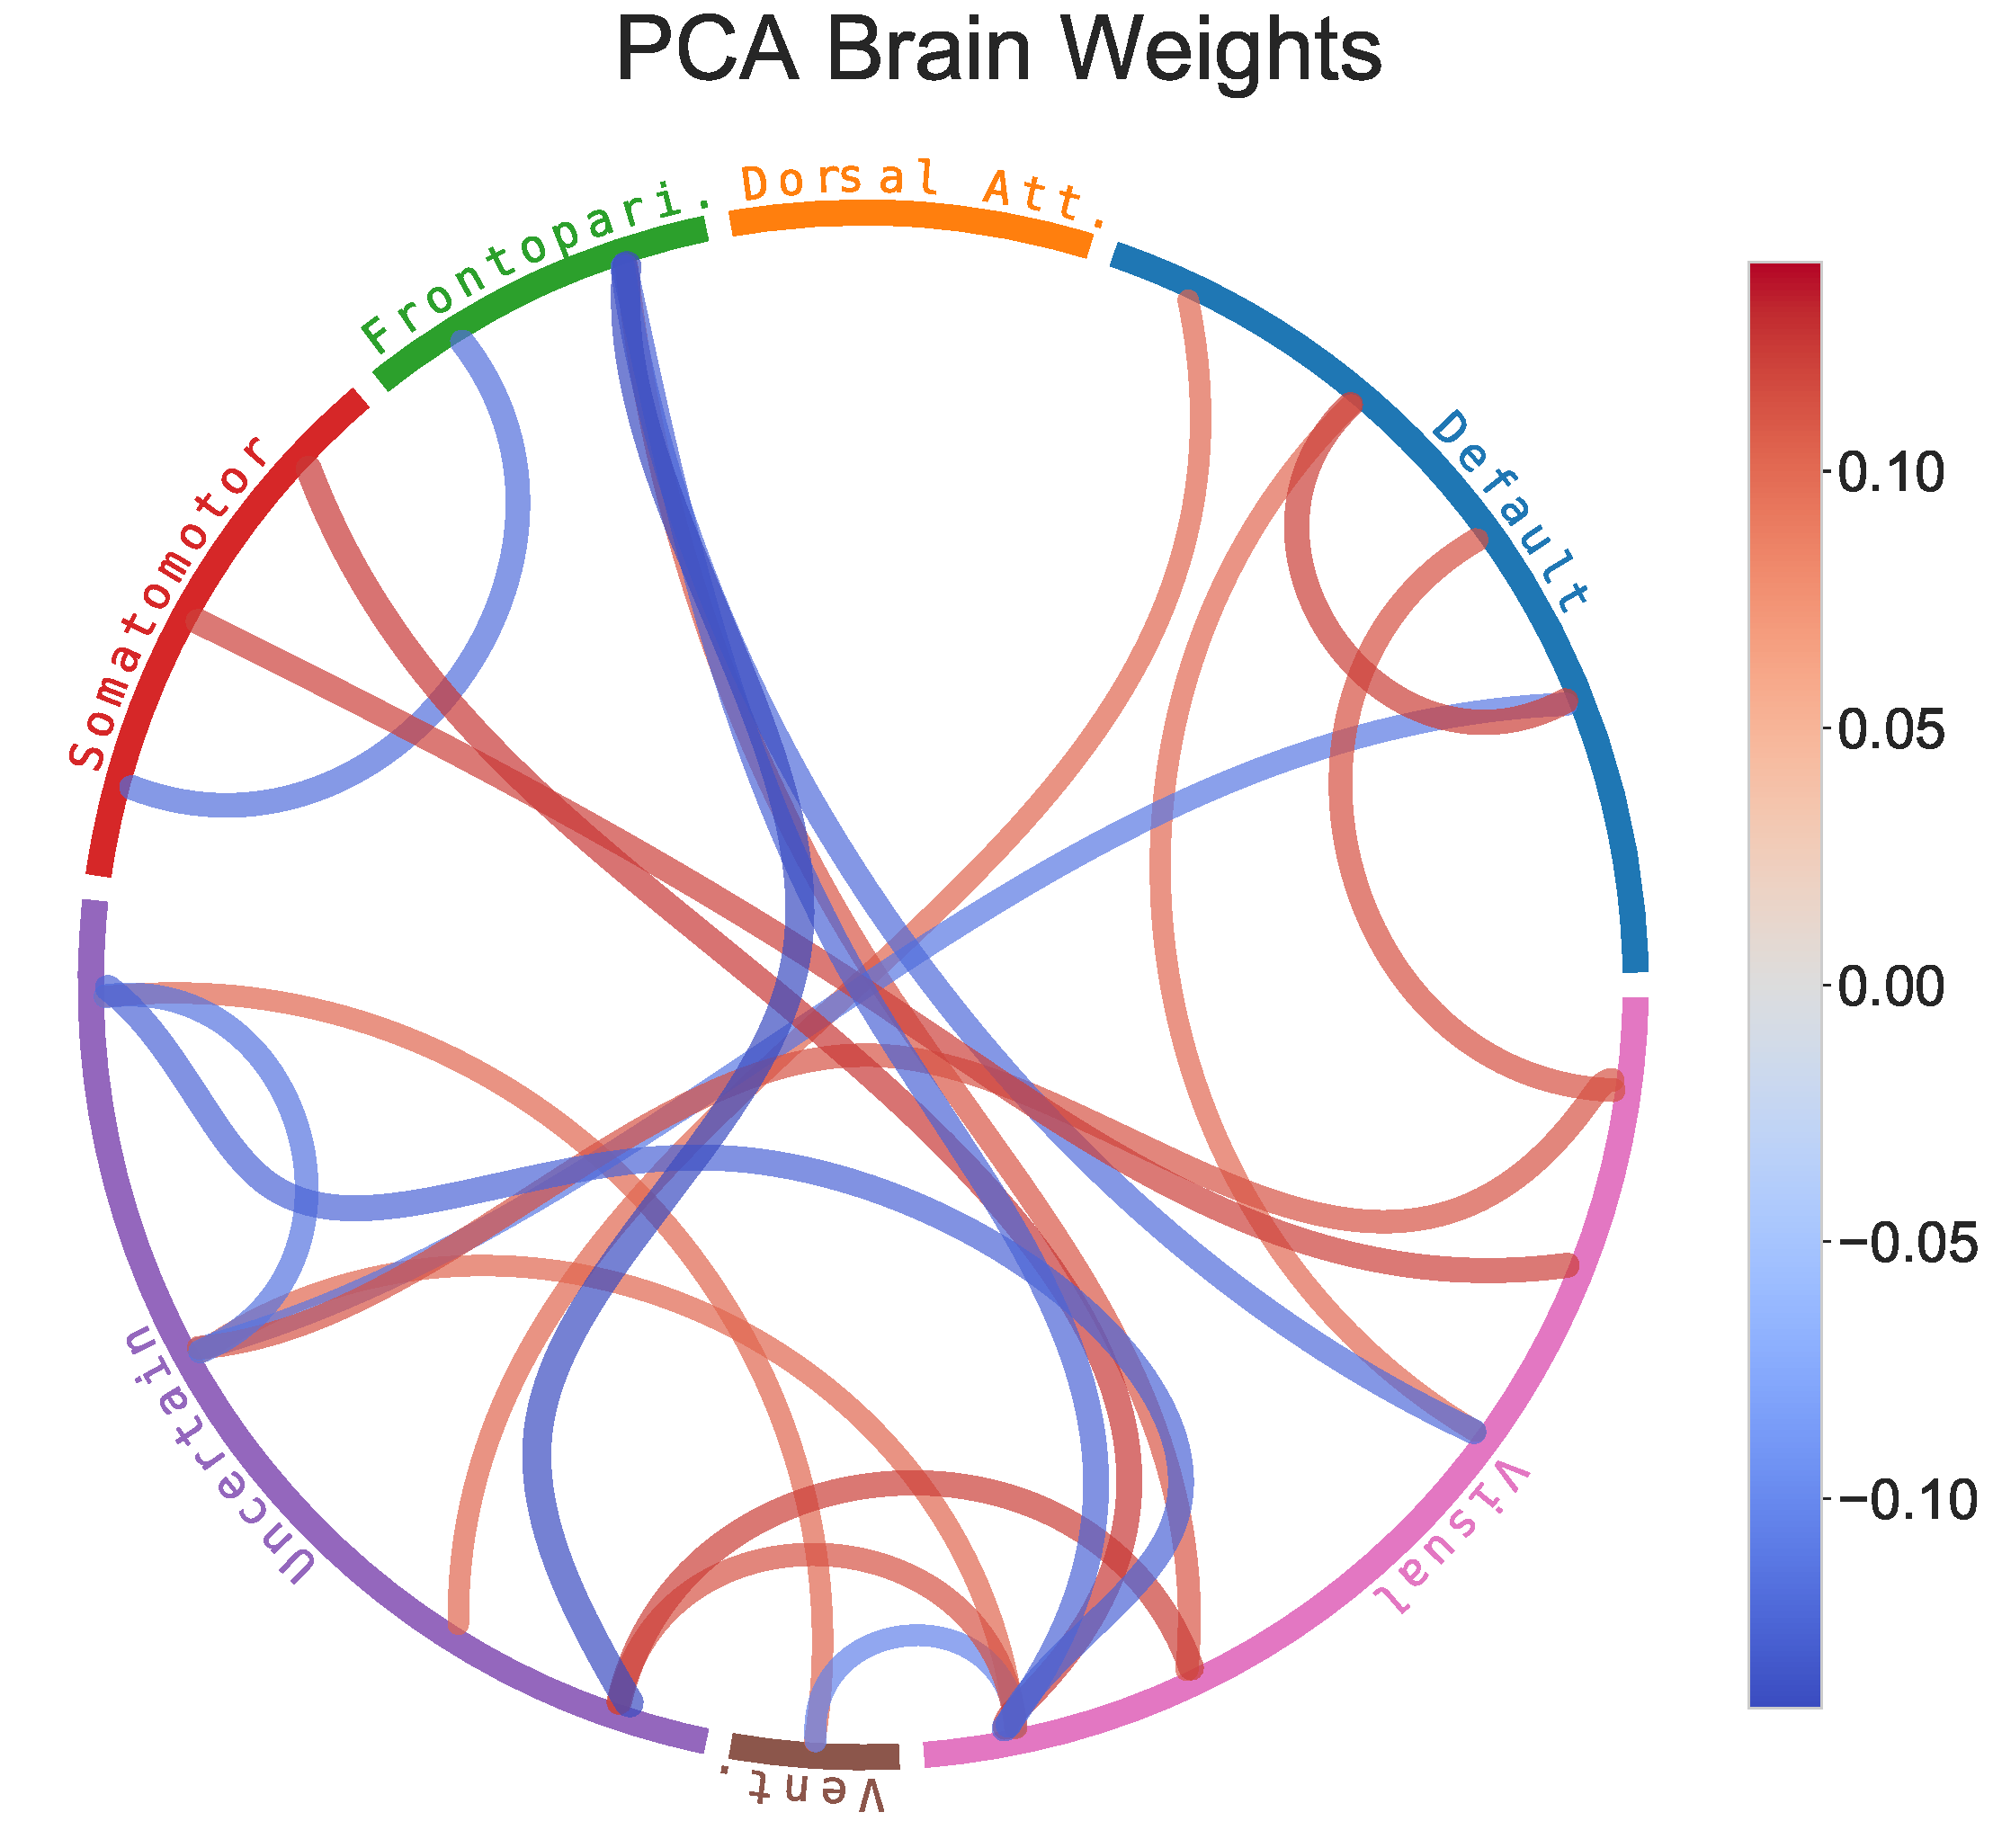
\includegraphics[width=0.49\linewidth]{figures/hcp/PCA brain weights}
    \caption{\textbf{HCP:} Chord diagrams of the top 8 positive and negative brain \gls{weights} for each model.}\label{fig:chord_weights}
\end{figure}

\subsubsection{Model Similarity}

In this section, we compare the models in terms of their similarity.
We can measure the pairwise similarity between two models by comparing their \gls{weights} and their \gls{representations}.
We can compare the \gls{weights} by computing the correlation between the \gls{weights} of the two models and we can compare the \gls{representations} by computing the correlation between the \gls{representations} of the two models.

In Figure~\ref{fig:brain-behaviour-scores-sim}, we plot the correlation between the brain and behaviour \gls{representations} for each model. 
We can see clearly that both PCA, PLS, and SPLS are all highly correlated in terms of their brain representations, revealing the bias of PLS towards the largest principal components.
On the other hand, in the behaviour space, the models are less correlated, with the exception of PLS and SPLS which are highly correlated with one another. 
There is however still substantial correlation between the PCA and PLS models.
The very low correlation between the Ridge CCA and Elastic Net models with the PCA model is evidence that there are stronger correlations outside of the first principal components.

In Figure~\ref{fig:brain-behaviour-weights-sim}, we similarly plot the correlation between the brain and behaviour \gls{weights} for each model. 
The story is similar, albeit with marginally lower correlations between the PLS and PCA-based models. Finally, in the weights space, the Ridge CCA and ElasticNet models are even less correlated with the PCA model.

\begin{figure}
    \centering
    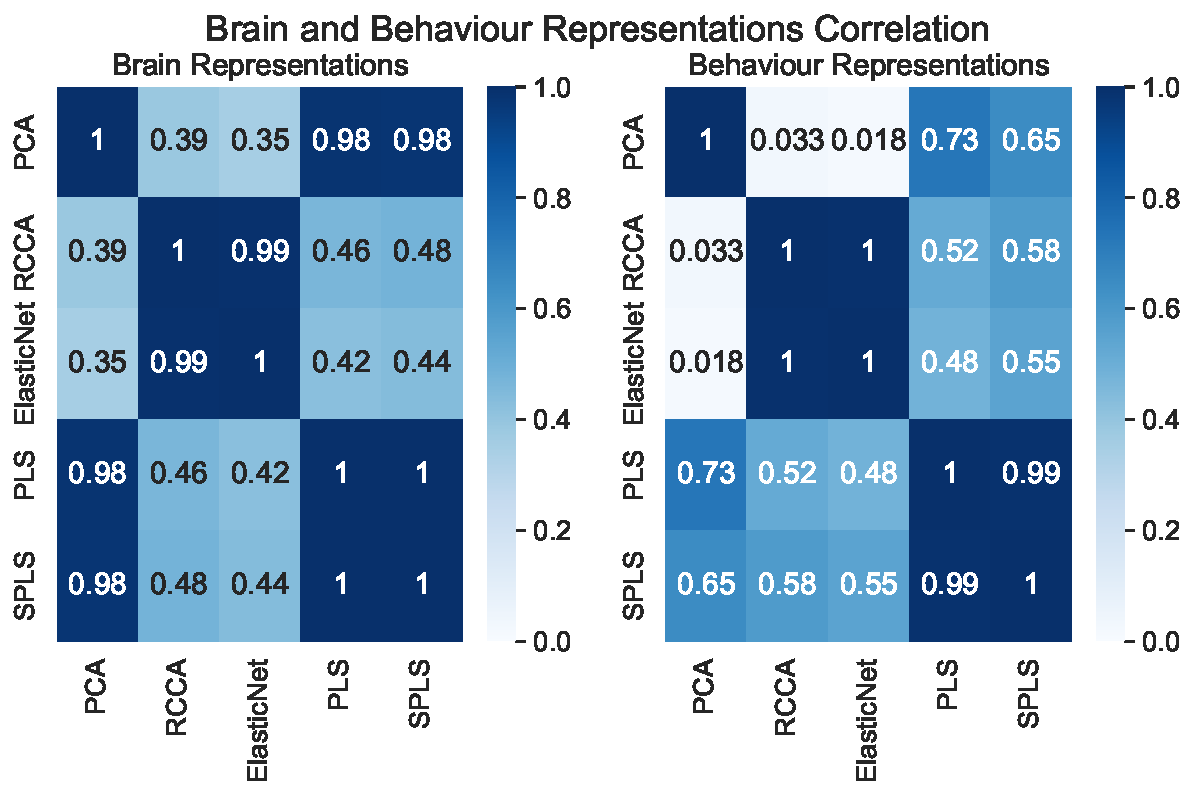
\includegraphics[width=0.8\linewidth]{figures/hcp/brain and behaviour scores correlation}
    \caption{\textbf{HCP:} Correlation between the brain and behaviour \gls{representations} for each model.}\label{fig:brain-behaviour-scores-sim}
\end{figure}

\begin{figure}
    \centering
    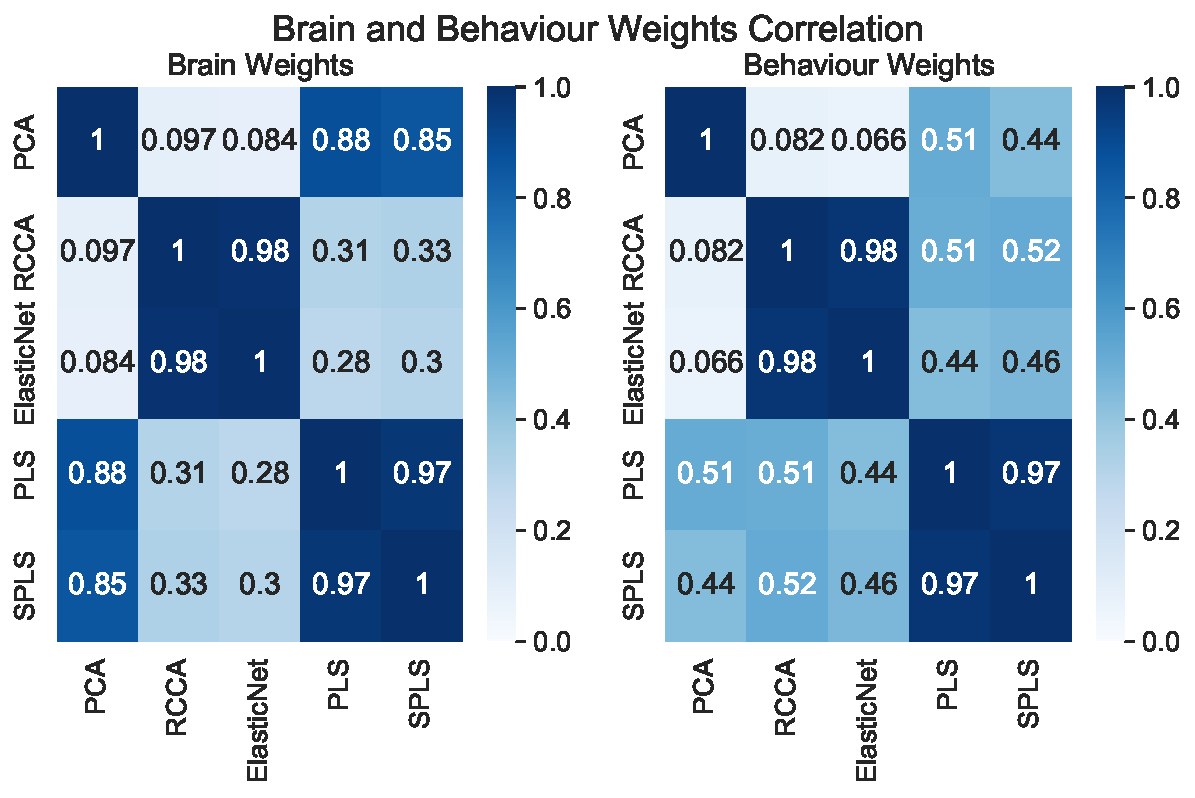
\includegraphics[width=0.8\linewidth]{figures/hcp/brain and behaviour weights correlation}
    \caption{\textbf{HCP:} Correlation between the brain and behaviour \gls{weights} for each model.}\label{fig:brain-behaviour-weights-sim}
\end{figure}


\subsection{\acrshort{adni} Results}\label{subsec:adni}

We now turn to the \acrshort{adni} data.

\subsubsection{Out of Sample Correlation}

In this experiment, the Elastic Net model outperformed all other models in terms of out-of-sample correlation (Figure~\ref{fig:performance}).
The RCCA model also outperformed the PLS and SPLS models while SPLS outperformed PLS.
Suprisingly, PCA performed almost as well as PLS.
This suggests that there is value in both tunable shrinkage and sparsity in this dataset.
It also reveals that the correlated signal between the brain structure and behavioural data is relatively much stronger than in the \acrshort{hcp} data.

\begin{figure}
    \centering
    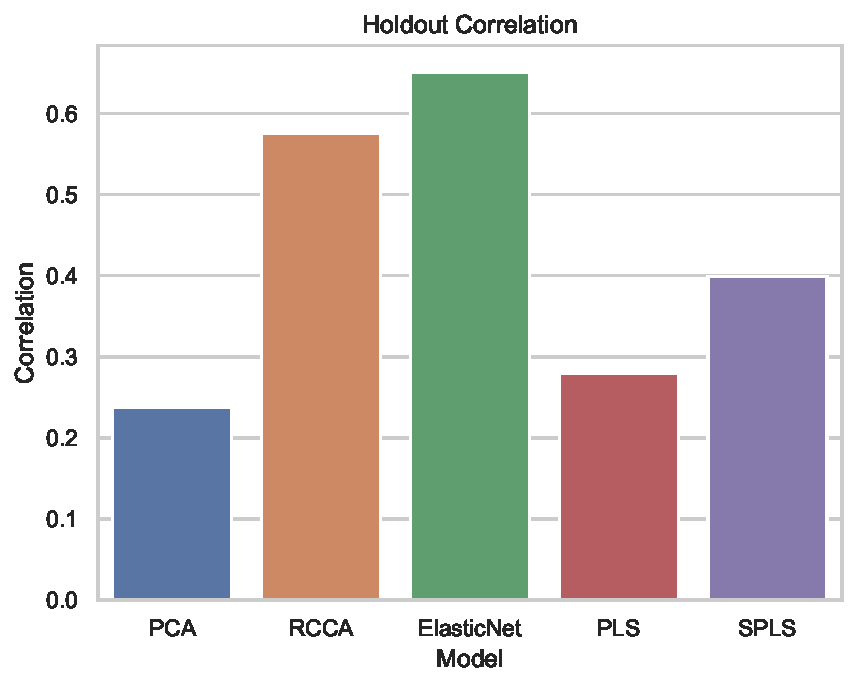
\includegraphics[width=0.5\linewidth]{figures/adni/holdout_correlations}
    \caption{\textbf{ADNI:} Out-of-sample canonical correlations for each model.}\label{fig:performance}
\end{figure}

\subsubsection{Sparsity of Weights}

Table~\ref{tab:brain-behaviour-weights-adni} once again shows the number of non-zero \gls{weights} for each model.
We can see that tuned SPLS and Elastic Net once again identify sparse weights.
In this case, the difference in performance is more convincing and suggests that this sparsity is less spuriously induced than for the \acrshort{hcp} data.
This is supported by the fact that Elastic Net and SPLS models find a similar level of sparsity in the brain weights.
On the other hand SPLS finds a much sparser set of behavioural weights.

\begin{table}
    \centering
    \caption{\textbf{ADNI:} Number of non-zero \gls{weights} for each model.}
    \begin{tabular}{|c|c|c|}
        \hline
        Model       & Brain Weights & Behaviour Weights \\
        \hline
        PCA         & 168130        & 31                \\
        RCCA        & 168130        & 31                \\
        Elastic Net & 59617         & 17                \\
        PLS         & 168130        & 31                \\
        SPLS        & 74995         & 10                \\
        \hline
    \end{tabular}\label{tab:brain-behaviour-weights-adni}
\end{table}

\subsubsection{Behaviour Weights}

As for the \acrshort{hcp} data, Figure \ref{fig:adni-beh} plots the top 8 positive and negative non-imaging \gls{weights} for each model.
Some of the identified behavioural \gls{weights} including a number of orientation tests are similar across all of the models, including even PCA.
This is indicative of the strong shared signal between the behavioural data and the brain structure data.
SPLS and Elastic Net both hone in on the orientation and recall tests in the weight space.
The RCCA and Elastic Net models are suprisingly different in the weight space, with the RCCA \gls{weights} on a couple of attention and calculation tests in addition to the ubiquitous orientation and recall tests.

\begin{figure}
    \centering
    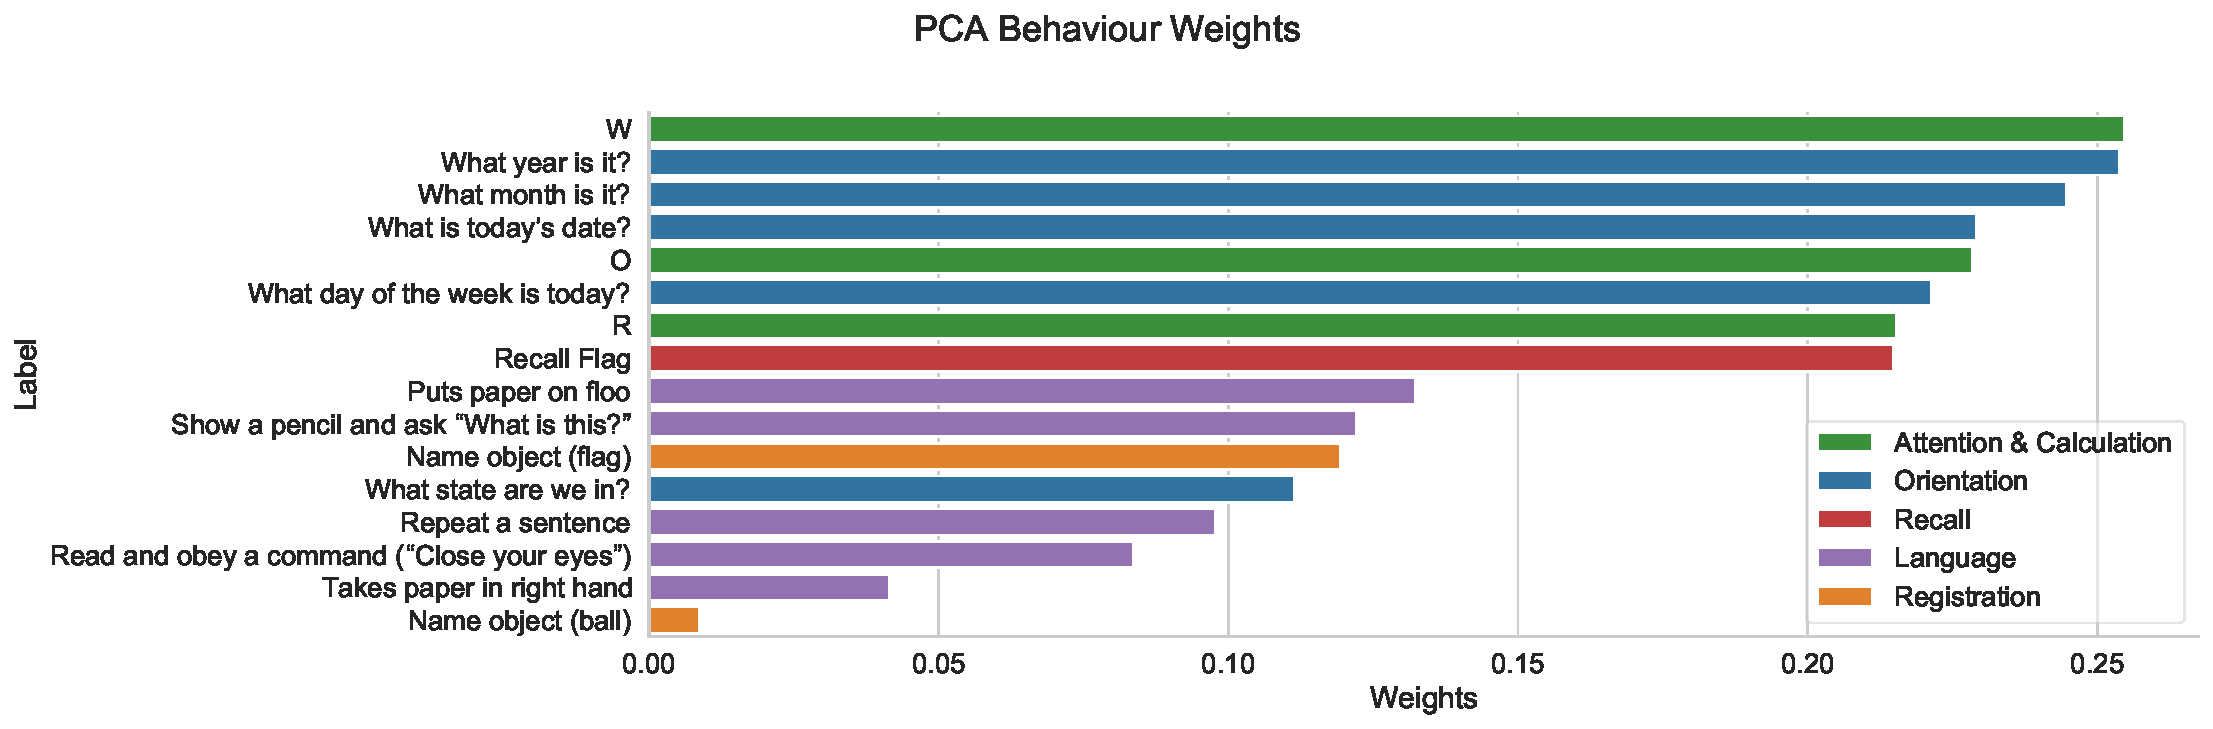
\includegraphics[width=0.8\linewidth]{figures/adni/PCA behaviour weights}
    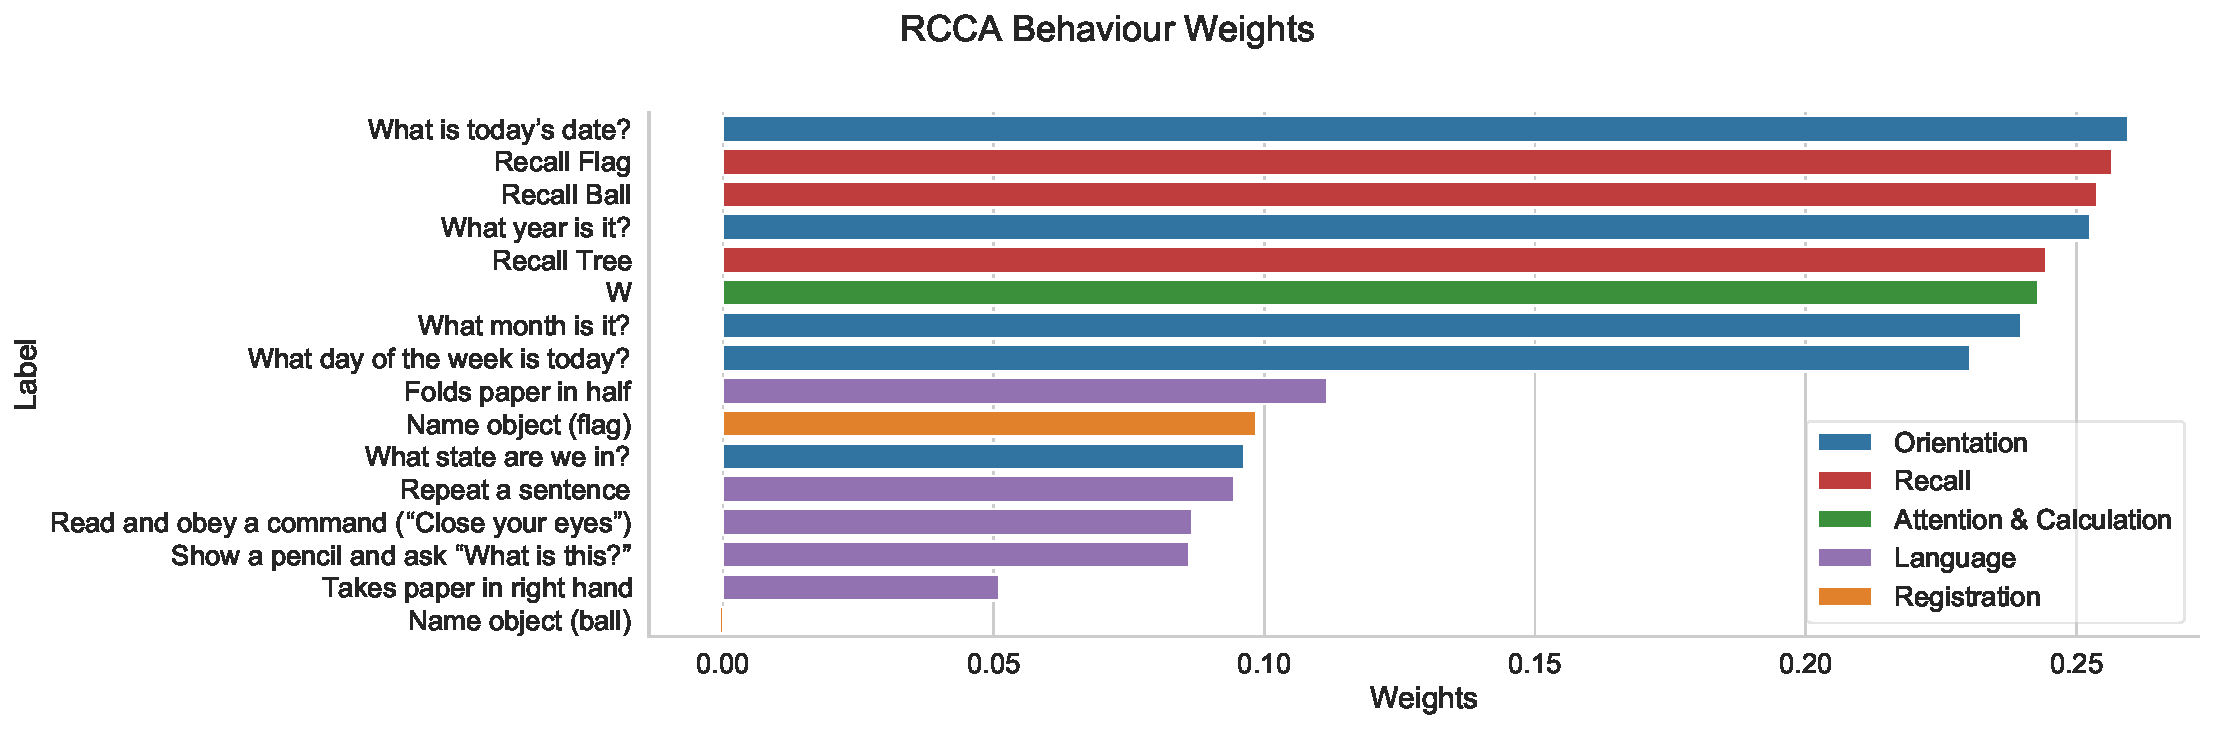
\includegraphics[width=0.8\linewidth]{figures/adni/RCCA behaviour weights}
    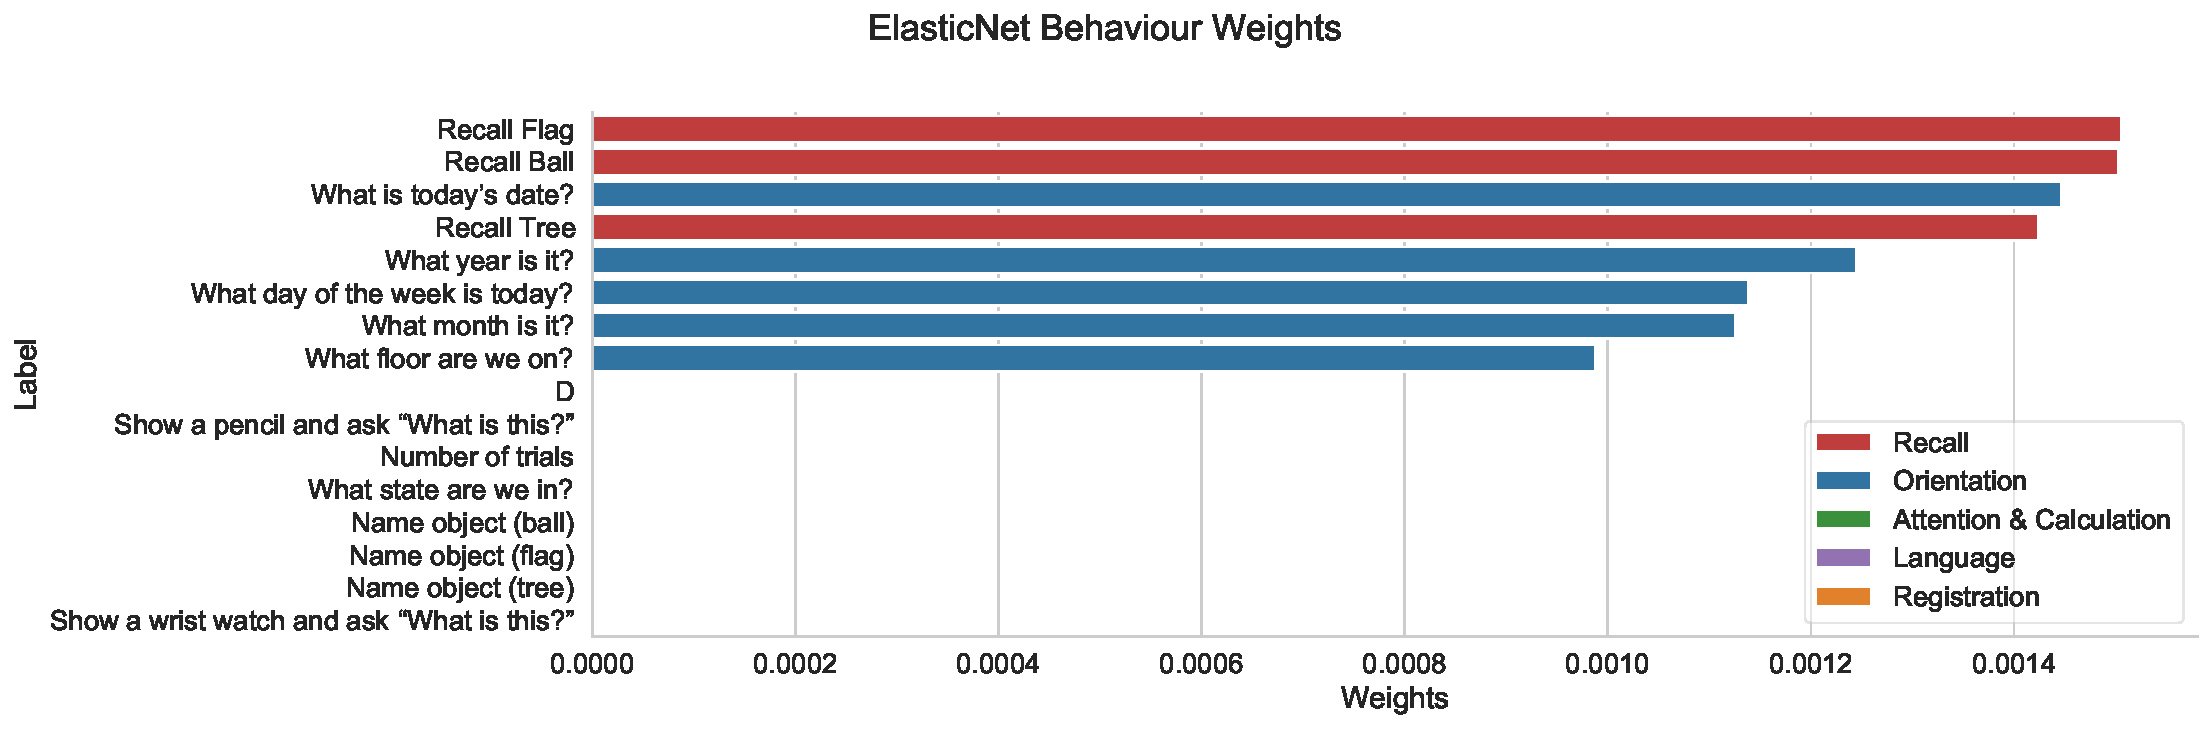
\includegraphics[width=0.8\linewidth]{figures/adni/ElasticNet behaviour weights}
    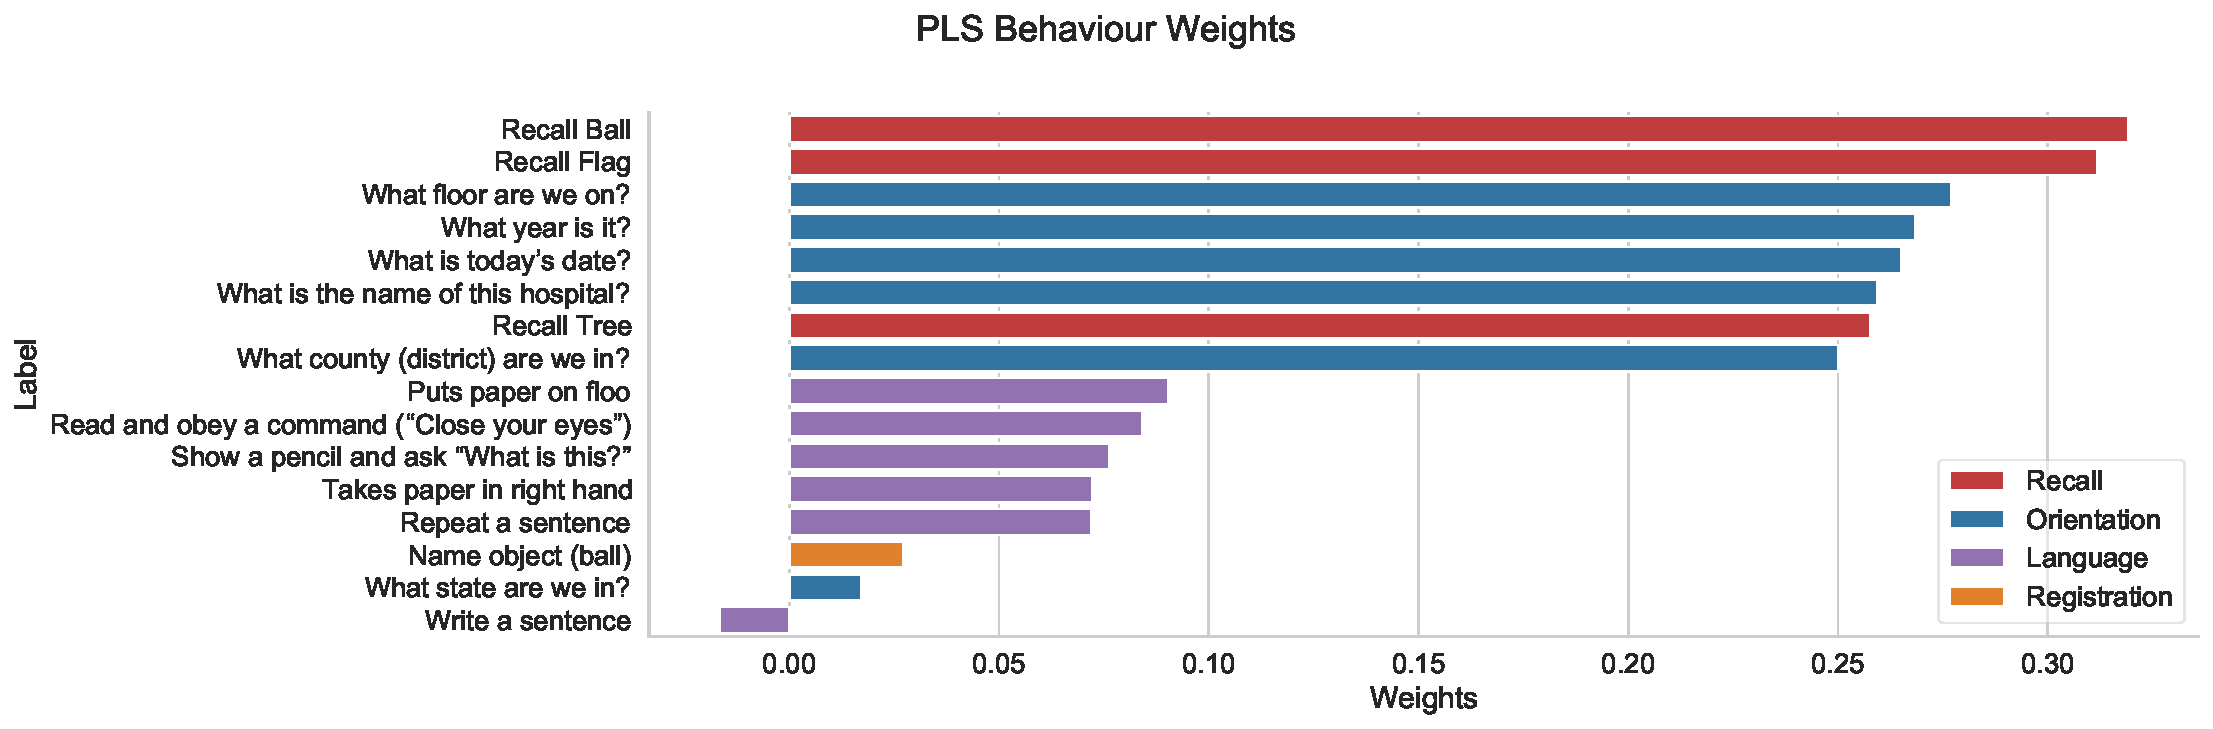
\includegraphics[width=0.8\linewidth]{figures/adni/PLS behaviour weights}
    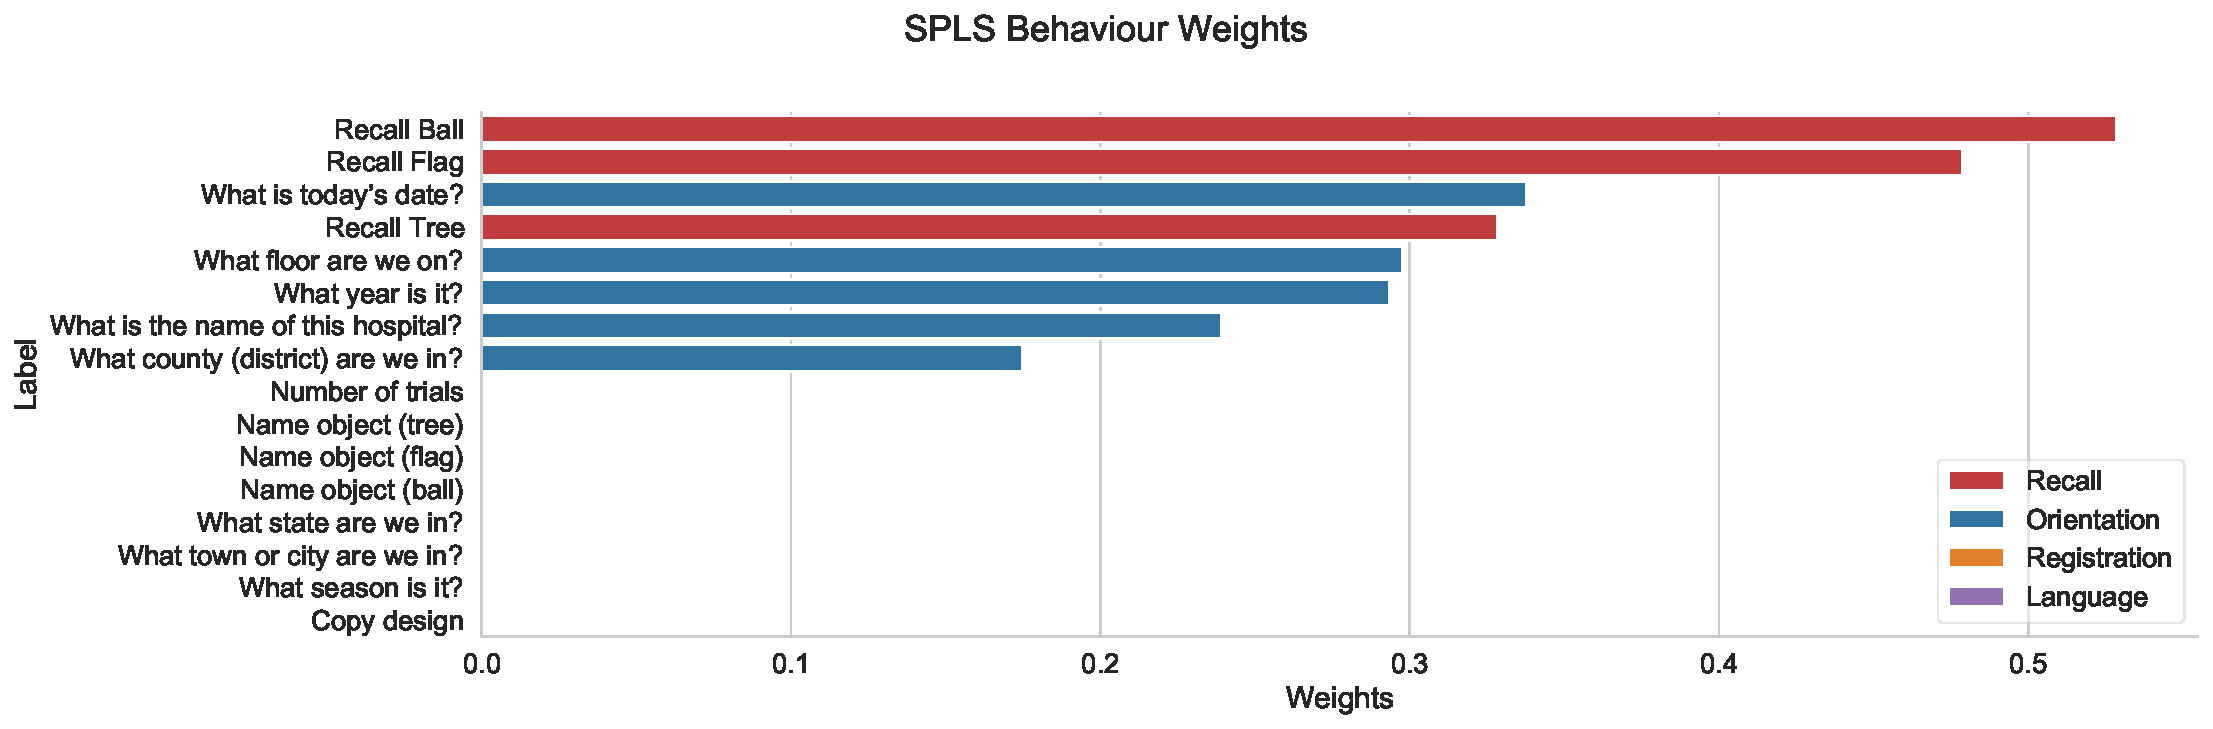
\includegraphics[width=0.8\linewidth]{figures/adni/SPLS behaviour weights}
    \caption{\textbf{ADNI:} Bar plots of the behaviour \gls{weights} for each model.}\label{fig:adni-beh}
\end{figure}

\subsubsection{Brain Structure Weights}

We plot the \gls{weights} as a mosaic plot with 3 slices in each direction in Figure~\ref{fig:adni-brain}.
Previous work using SPLS with the \acrshort{adni} dataset identified the same striking pattern of \gls{weights} with the model strikingly selecting the hippocampal weights\cite{monteiro2016multiple}.
The Elastic Net has a less visually appealing selection of weights, with a honeycomb pattern near the edges of the brain and likewise for RCCA.
It is noticeable that PCA, PLS and SPLS both \gls{weights} in the same direction whereas RCCA and Elastic Net weight different regions with opposite signs.

\begin{figure}
    \centering
    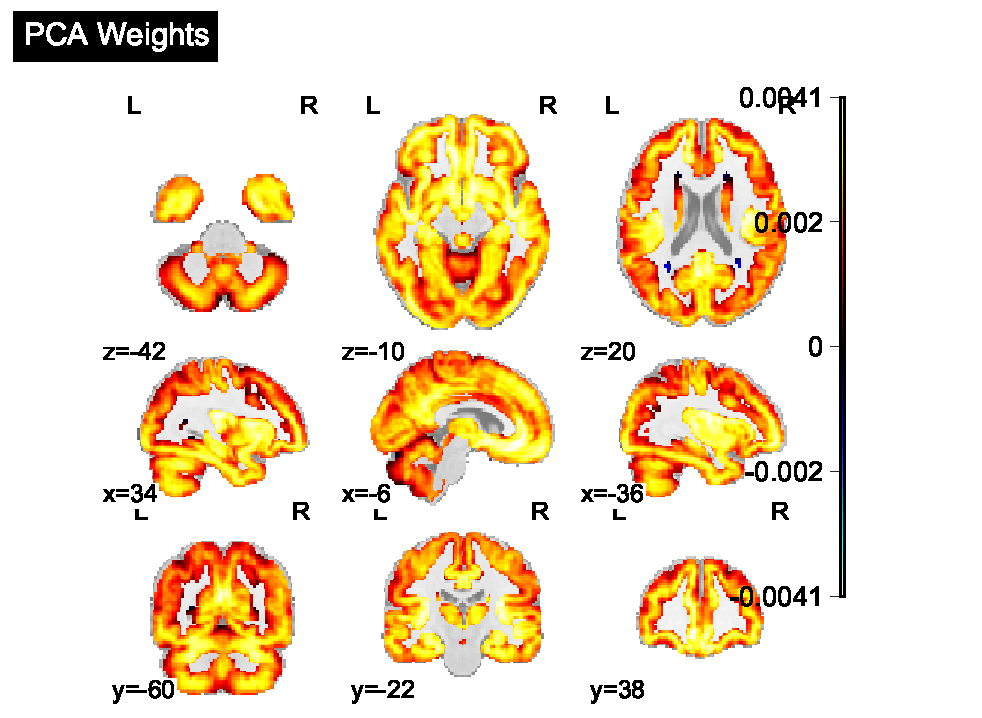
\includegraphics[width=0.45\linewidth]{figures/adni/PCA brain weights mosaic}
    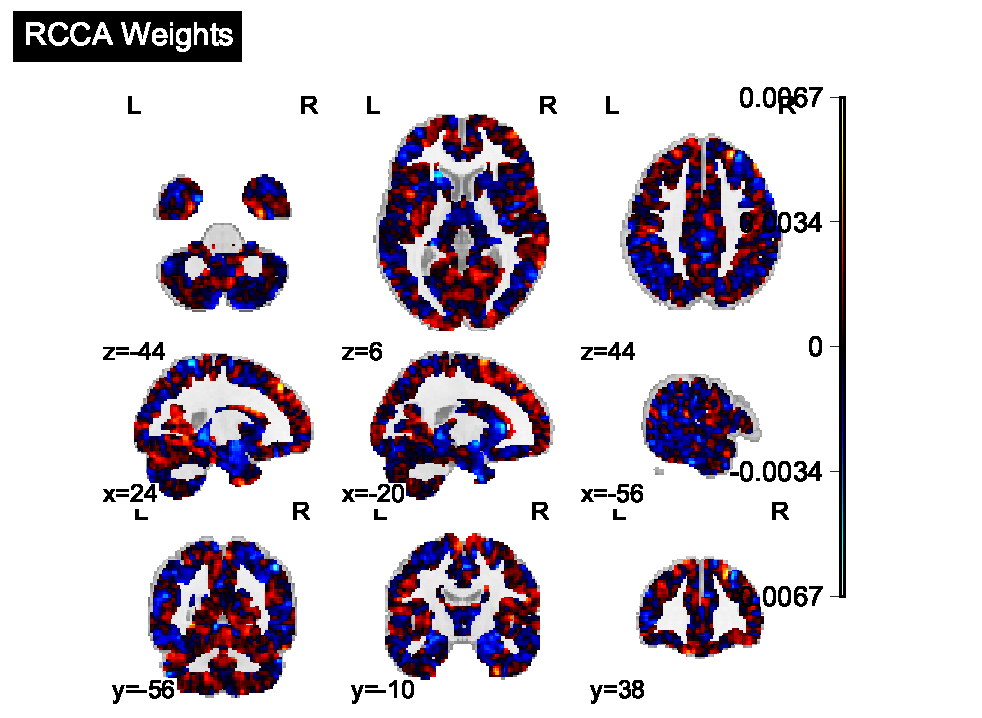
\includegraphics[width=0.45\linewidth]{figures/adni/RCCA brain weights mosaic}
    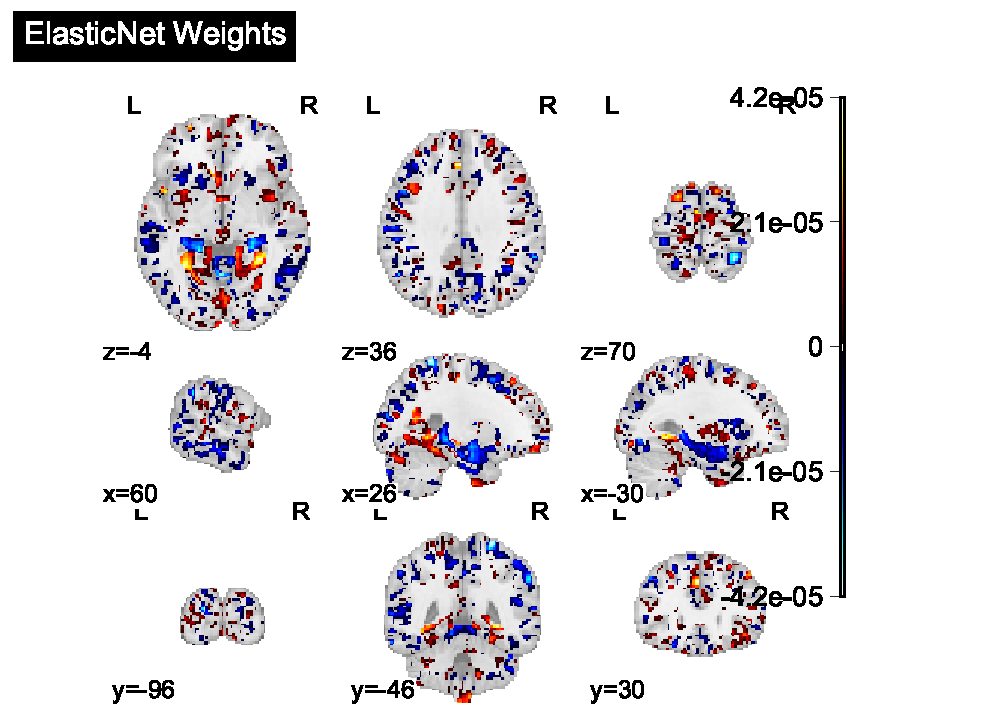
\includegraphics[width=0.45\linewidth]{figures/adni/ElasticNet brain weights mosaic}
    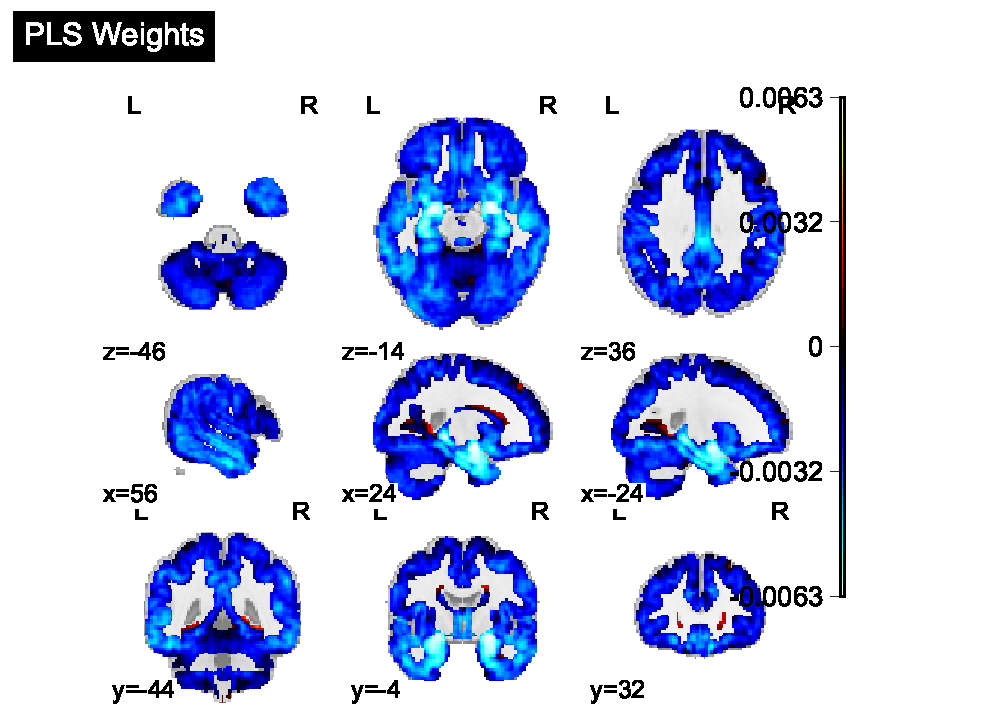
\includegraphics[width=0.45\linewidth]{figures/adni/PLS brain weights mosaic}
    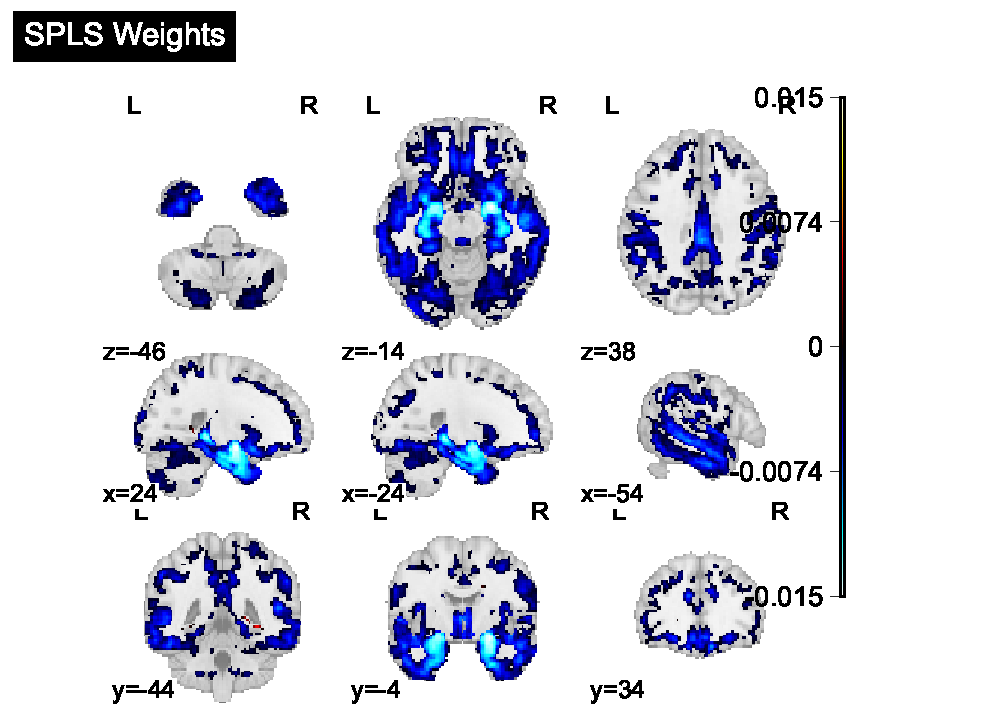
\includegraphics[width=0.45\linewidth]{figures/adni/SPLS brain weights mosaic}
    \caption{\textbf{ADNI:} Statistical maps of brain structure weights for each model.}
\end{figure}

\subsubsection{Model Similarity}

In this section, we once again compare the models in terms of their similarity.
In Figure~\ref{fig:brain-behaviour-scores-sim-adni}, we can see that all of the models are highly correlated in terms of their behaviour \gls{representations}.
The brain \gls{representations} are less correlated, but once again PCA, PLS, and SPLS are highly correlated with one another and less correlated with the Ridge CCA and Elastic Net models.

Suprisingly, in Figure~\ref{fig:brain-behaviour-weights-sim-adni}, we can see that the weights in both views are less correlated. This is particularly true for the brain \gls{weights} where PCA exhibits a very low correlation with Ridge CCA and Elastic Net.

\begin{figure}
    \centering
    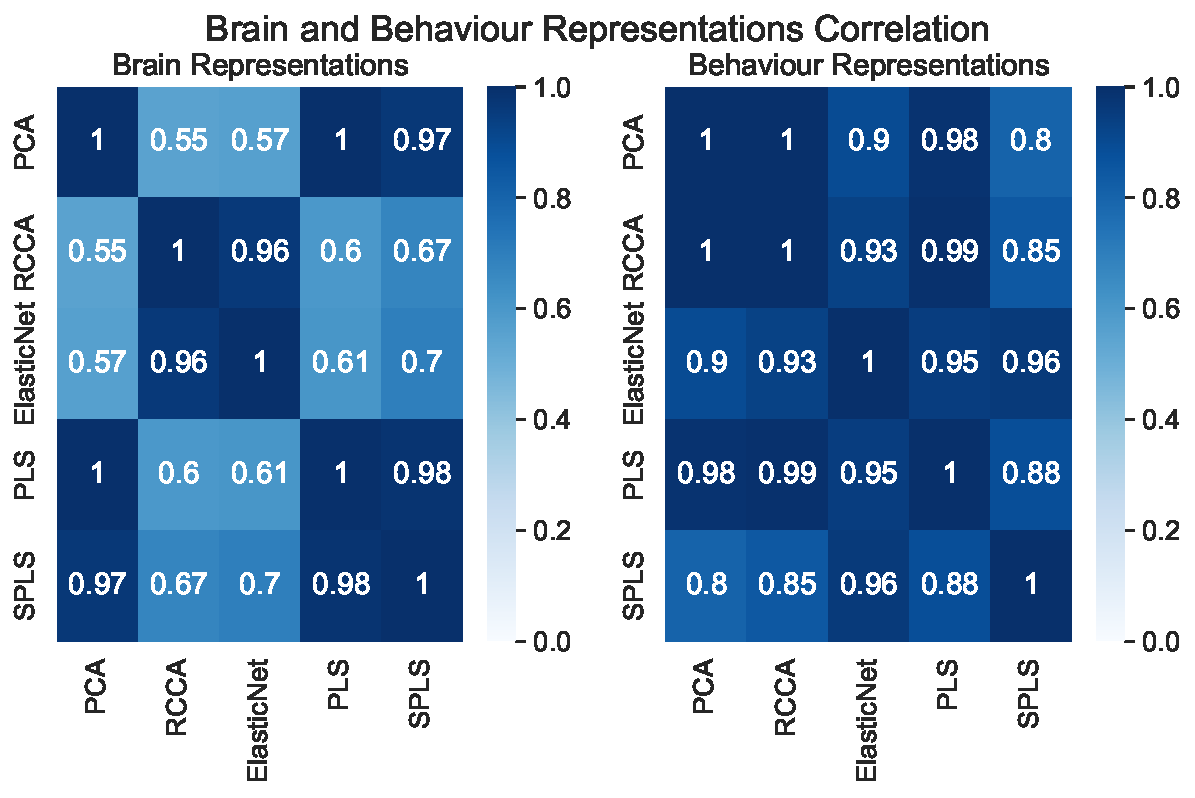
\includegraphics[width=0.8\linewidth]{figures/adni/brain and behaviour scores correlation}
    \caption{\textbf{ADNI:} Correlation between the brain and behaviour \gls{representations} for each model.}\label{fig:brain-behaviour-scores-sim-adni}
\end{figure}

\begin{figure}
    \centering
    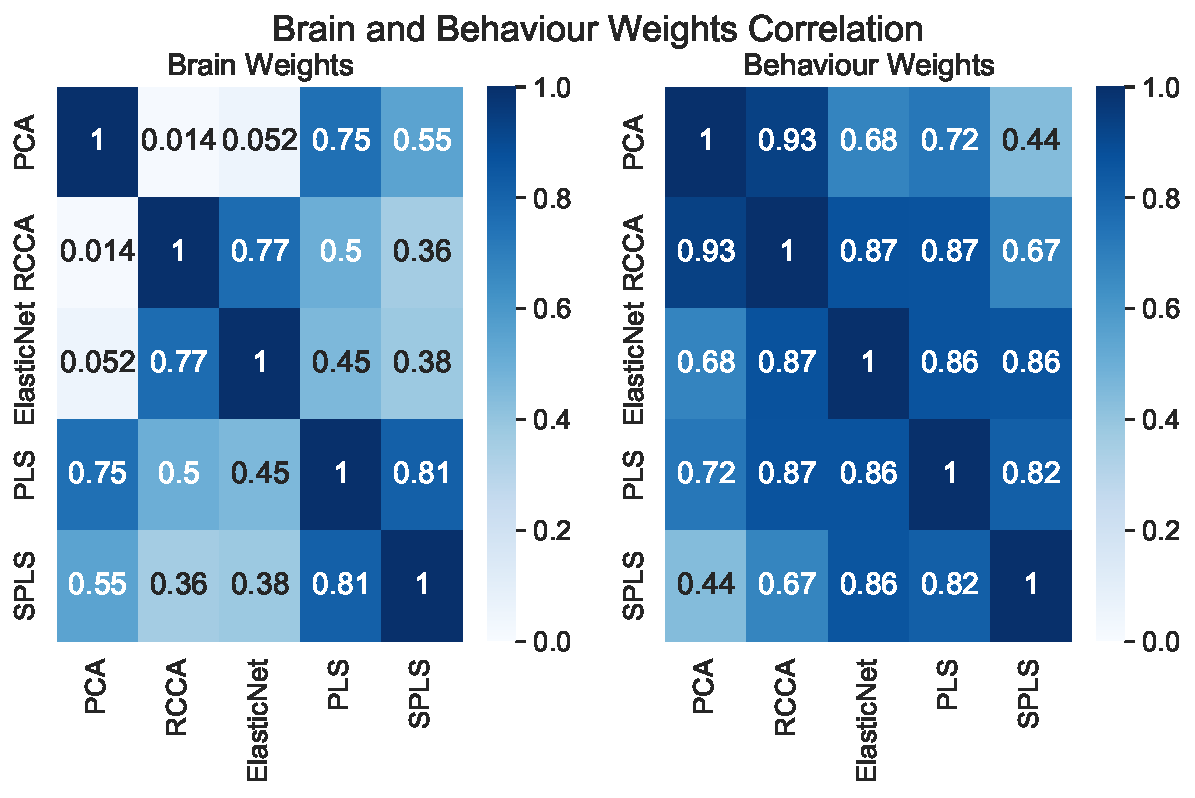
\includegraphics[width=0.8\linewidth]{figures/adni/brain and behaviour weights correlation}
    \caption{\textbf{ADNI:} Correlation between the brain and behaviour \gls{weights} for each model.}\label{fig:brain-behaviour-weights-sim-adni}
\end{figure}

\subsection{Timings}

Finally, we consider the timings of the different models.
This is an important metric because one of the main reasons for the popularity of SPLS is its speed and therefore convenience.
Figure \ref{fig:timings} shows an estimate of the time taken to fit each model for each complete training dataset over 10 runs.
We can see clearly that the Elastic Net is much slower than the other models when using the high dimensional \acrshort{adni} data.
Despite also being an iterative algorithm, the SPLS model is much faster than the Elastic Net and only slightly slower than the PLS and RCCA models which call optimised solvers in C.
Since PLS and RCCA both use PCA preprocessing for efficiency, it is unsuprising that PCA is the fastest model.

\begin{figure}
    \centering
    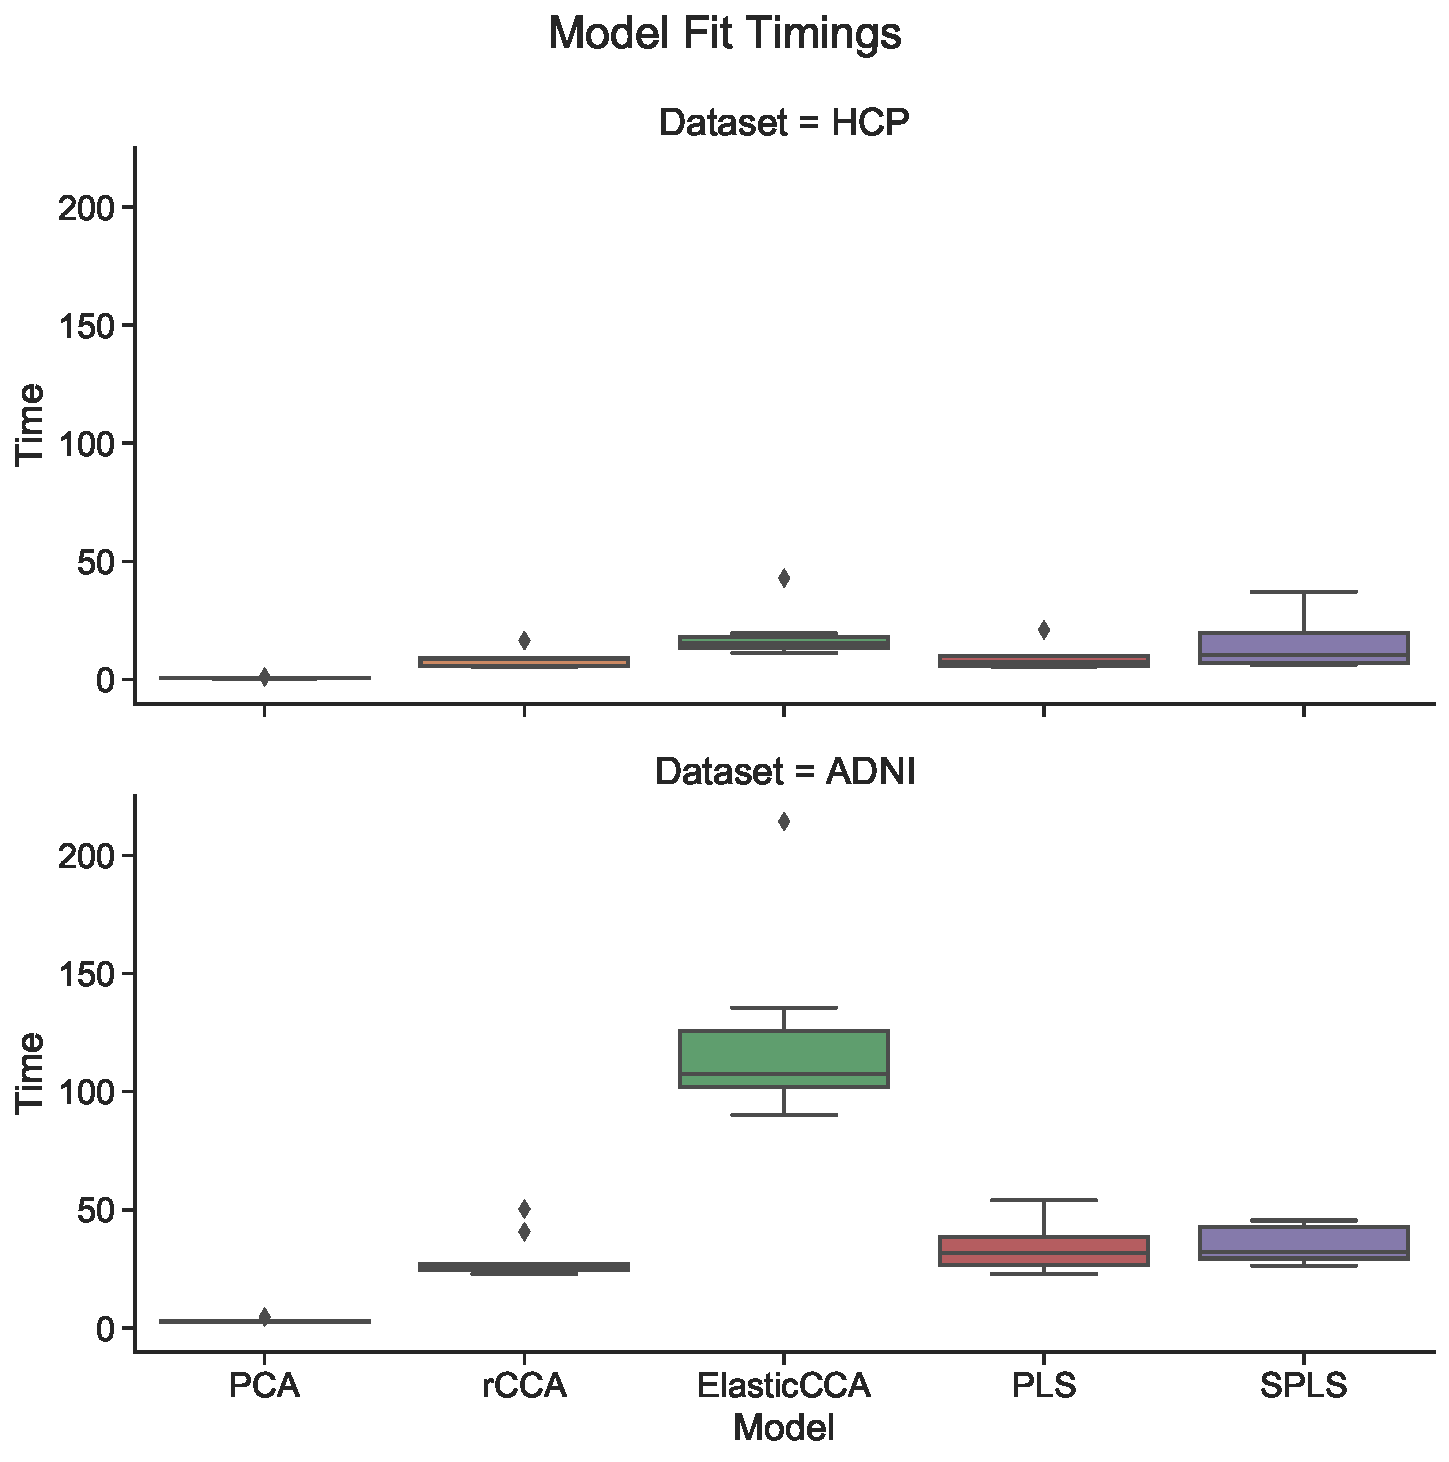
\includegraphics[width=0.45\linewidth]{figures/model_fit_timings}
    \caption{Time taken to fit each model.}\label{fig:timings}
\end{figure}

\section{Discussion and Limitations}

In this section, we discuss the implications of our findings as well as the limitations of our study and the proposed FRALS method, some of which we address in later chapters of this thesis.

\subsection{Discussion}

\paragraph{Ridge CCA is typically much better than PLS across datasets:} Our results show that Ridge CCA is typically much better than PLS across datasets.
Much like regularised regression, it is unusual to need to use maximal ridge regularisation even in high dimensions.
This means that while PLS might be more stable for a given dataset, it is not necessarily more stable across random samples from the same population.

\subsection{FRALS Limitations}
While FRALS offers promising performance in terms of out-of-sample correlation, it does come with significant drawbacks, the most noteworthy being its computational inefficiency.
Below, we outline the primary factors contributing to the slow speed of FRALS and provide some insights into the computational bottlenecks.

\paragraph{Changing Regression Targets}\label{subsec:changing-regression-targets}
Adding to the computational burden is the fact that the regression targets, i.e., the projections of the other view, are not static but change dynamically throughout the algorithm's run.
Each update to the least squares solution consequently alters the global objective, leading to a constantly shifting landscape that the algorithm needs to navigate.
This also leads to a significant amount of redundant computation, as the algorithm needs to recompute the least squares solution for each view at each iteration.

\paragraph{Computational Time}\label{subsec:computational-time}

The primary bottleneck in FRALS is the computation of the least squares solution.
For each iteration of the algorithm, we need to compute the least squares solution for each view.
This is a computationally expensive operation.
It is the primary factor contributing to the slow speed of FRALS (depending on the experiment around 10 times slower than Ridge CCA).

\section{Conclusion}\label{sec:conclusion}

In this chapter, we introduced the Flexible Regularised Alternating Least Squares (FRALS) framework for CCA\@.
We used the FRALS framework to implement Elastic Net CCA\@.
We then compared the performance of Elastic Net CCA with other CCA variants on two datasets: the \acrshort{hcp} and \acrshort{adni}.
We found that Elastic Net CCA outperformed other CCA variants on both datasets but that the performance of Elastic Net CCA was similar to Ridge CCA on the \acrshort{hcp} dataset.
However, we found that Elastic Net CCA was much slower than other CCA variants.

\chapter{Regularization and the Interpretation of CCA Weights and Loadings}\label{chap:als}
\minitoc
% chktex-file 44
% chktex-file 3


\section{Introduction}\label{sec:introduction}

The application of Canonical Correlation Analysis (CCA) methods to practical problems often involves two key aspects: predicting latent variables associated with different views, and understanding the nature of the relationship between these views.
This dichotomy in goals bears resemblance to the distinction between machine learning and probabilistic or statistical approaches to the CCA problem.
Machine learning approaches prioritize (out-of-sample) prediction of latent variables for downstream tasks, while statistical approaches seek to infer the data generation process from latent variables to the observed data.
Notably, the probabilistic approach to CCA focusses on the forward model from latent variables to observed data, while the machine learning approach focusses on the inverse model from observed data to latent variables.
As a result the probabilistic CCA is parameterized by the \textit{loadings} (parameters that transform latent variables to observed data), while the machine learning approach is parameterized by \textit{weights} (parameters that transform obsevred data to latent variables).
We would ideally like to have the best possible prediction of the latent variables, while also being able to interpret the model and understand the relationship between the views.
This implies that we would like to have models which are both good at prediction and have interpretable loadings that we can use to understand the relationship between the views via the data generation process.
The importance of the loadings (associated with the `forward' model from latent variables to observed data) instead of weights (associated with the `backward' model from observed data to latent variables) for interpretability was highlighted by \cite{haufe2014interpretation} for linear models including SVM and Lasso, along with methods for transforming `backward' weights to `forward' loadings.
We contribute to this line of work by demonstrating a similar relationship between the loadings and weights of CCA models, and showing that the loadings are more interpretable than the weights.

In this chapter, we reexamine the relationship between machine learning and probabilistic CCA approaches using simulated data.
We demonstrate that these approaches are more aligned than previously thought.
While sparse regularization of CCA weights can lead to sparse estimates of generative model loadings in some conditions, it doesn't always ensure sparse loadings, especially under anisotropic noise (i.e. noise correlated between features).
Furthermore, regularization can enhance performance in low SNR scenarios, but using the PLS objective can introduce bias, emphasizing dominant principal components and overshadowing subtler correlations.

\section{Background:Generative Perspectives on CCA}\label{sec:background}

Understanding the data generation process in Canonical Correlation Analysis (CCA) and Partial Least Squares (PLS) is pivotal for many reasons.
It influences the choice of appropriate models, evaluation metrics, and sheds light on the underlying structure and dependencies between views.
Probabilistic formulations provide a principled framework to understand this process, helping us gauge the assumptions we make and the limitations these impose.

\subsection{Probabilistic CCA and GFA (Explicit Latent Variable Models}\label{subsubsec:a-probabilistic-latent-variable-perspective-on-cca}

Consider the graphical model depicted in Figure~\ref{fig:mentalhealthselfsupervised}.
It comprises two distinct views: a neuroimaging modality and a behavioral modality.
Both views are assumed to originate from a common latent variable, representing the severity of a mental health condition.
The neuroimaging modality is generated via a linear model with added noise, while the behavioral modality similarly arises from a linear model with noise.
Consequently, the brain and behavioral modalities exhibit correlation since they both derive from the same latent variable.
In a statistical sense, they are conditionally independent, given the latent variable.

\begin{figure}
    \centering
    \tikz{
        % nodes
        \node[latent, align=center, minimum size=2cm] (Z) {Severity\\z};
        %
        \node[obs, below left=of Z, minimum size=2cm, align=center] (x1) {Brain\\$x^{(1)}$};
        \node[obs, below right=of Z, minimum size=2cm, align=center] (x2) {Behaviour\\$x^{(2)}$};
        % edges
        \edge{Z} {x1}
        \edge{Z} {x2}}
    \caption[Latent Variable Model of Mental Health]{\textit{\textbf{Latent Variable Model of Mental Health:}} From this perspective the neuroimaging modality and behavioural data are both considered to have been generated with distributions conditioned on the severity of a mental health condition}\label{fig:mentalhealthselfsupervised}
\end{figure}

The distributions of the two views are given by:

\begin{align}
    z& \sim \mathcal{N}(0, I)\\
    x\sps{i} & \sim \mathcal{N}(W\sps{i} z + \mu\sps{i}, \Psi\sps{i})
\end{align}

Where \(z\) represents the latent variable (disease severity), \(x\sps{i}\) represents the $i^{\text{th}}$ view, \(W\sps{i}\) represents the model loadings, \(\mu\sps{i}\) represents the mean, and \(\Psi\sps{i}\) represents the noise covariance matrix for the $i^{\text{th}}$ view.
Notice that if it were not for the view-specific noise, the two views would be perfectly correlated subject to a linear transformation.

\citep{bach2005probabilistic} showed that the maximum likelihood solution for this model is equivalent to the solution of the CCA problem in the sense that the loadings are the same as the CCA weights multiplied by the covariance:

\begin{align}\label{eq:probabilistic-cca}
    \hat{W}\sps{i} = \Sigma_{ii} \hat{U}\sps{i} R
\end{align}

Where $R$ is an arbitrary rotation matrix and $\hat{U}\sps{i}$ is the matrix of CCA weights for the $i$th view.
This implies that for invertible covariance matrices, we can access the `true' CCA weights by multiplying the loadings by the inverse of the covariance matrix:

\begin{align}
    \hat{U}\sps{i} = \Sigma_{ii}^{-1} \hat{W}\sps{i}
\end{align}

In practice we do not have access to the covariance matrices $\Sigma_{ii}$, so we must estimate them from the data using the sample covariance matrices $\hat{\Sigma}_{ii}$.

Notice that for Identity covariance matrices, the CCA weights are the same as the loadings.
Otherwise, there is a linear transformation between the two.
For singular covariance matrices, the CCA weights are not uniquely defined.

Moreover, the mean of the posterior distribution of the latent variables is proportional to the mean of the CCA scores\citep{klami2013bayesian}.
Group Factor Analysis (GFA) is a closely related model that assumes diagonal covariance in $\Psi\sps{i}$:

\begin{align}
    z& \sim \mathcal{N}(0, I)\\
    x\sps{i} & \sim \mathcal{N}(W\sps{i} z, \sigma\sps{i}I)
\end{align}

An interesting feature of the GFA model is that as the noise level approaches zero, the marginal distribution of the views is the same as the probabilistic PCA model for each view~\citep{tipping1999probabilistic}.
This suggests that for small noise levels, we should in fact be able to recover much of the mutual information between the views by using PCA on each view separately.
For this reason, we will use and recommend PCA as a baseline in our later experiments.
Because the diagonal covariance assumption makes inference computationally cheaper, this line of work has been able to extend to incorporate sparsity on the loadings\citep{virtanen2011bayesian} as well as missing data~\citep{ferreira2022hierarchical}.

By marginalizing out the latent variables of the generative CCA and GFA models, we can write down the joint distribution of the two views:

\begin{align}
    \begin{bmatrix} X\sps{1} \\ X\sps{2} \end{bmatrix} \sim \mathcal{N} \left( \begin{bmatrix} \mu\sps{1} \\ \mu\sps{2} \end{bmatrix}, \begin{bmatrix} W\sps{1}W\spstop{1} + \Psi_1 & W\sps{1}W\spstop{2} \\ W\sps{2}W\spstop{1} & W\sps{2}W\spstop{2} + \Psi_2 \end{bmatrix} \right)
\end{align}

Importantly, this shows us that the true covariance in each view is a function of the loadings and the noise covariance matrix.
Specifically, the covariance matrix of the $i^{\text{th}}$ view is given by:

\begin{align}
    \Sigma_{ii} = W\sps{i}W\spstop{i} + \Psi_i
\end{align}

While these generative models are well-grounded in biological processes and provide a clear latent variable perspective, their application in practice is limited compared to classical CCA.
This is primarily due to their computational intensity and the need for a careful selection of priors.
Moreover, while these models can generate data with sparse loadings, generating data with sparse weights is challenging due to the dependence of CCA weights on the covariance matrices of the views.

\subsection{A Joint Covariance Matrix Perspective (Implicit Latent Variable Model)}\label{subsubsec:a-joint-covariance-matrix-perspective}

In contrast to the explicit latent variable models discussed earlier, the joint covariance matrix perspective offers an implicit approach to understanding the data generation process.
This method focuses on the covariance matrices of the views, rather than directly modeling latent variables.
A key advantage of this perspective, particularly noted in the sparse CCA literature, is its ability to generate data with sparse weights.
This is achieved by constructing the joint covariance matrix of the two views as follows:

\begin{align}\label{eq:covariance}
    \begin{bmatrix} X\sps{1} \\ X\sps{2} \end{bmatrix} \sim \mathcal{N} \left( \begin{bmatrix} 0 \\ 0 \end{bmatrix}, \begin{bmatrix} \Sigma_{11} & \Sigma_{12} \\ \Sigma_{21} & \Sigma_{22} \end{bmatrix} \right)
\end{align}

Where $\Sigma_{11}$ and $\Sigma_{22}$ are the within-view covariance matrices and $\Sigma_{12}$ and $\Sigma_{21}$ are the between-view covariance matrices.

This has the advantage of allowing us to control the within-view covariance and therefore test the methods under specific conditions.
The process was first described by Chen~\citep{chen2013sparse} and further explained by~\citep{suo2017sparse}.

We can control the true signal by setting the active variables and correlations in the between-view covariance matrices $\Sigma_{12}$ and $\Sigma_{21}$.
Specifically we construct the between-view covariance matrices as follows:

\begin{align}
    \Sigma_{12}=\sum_{k=1}^{K}\rho_k\Sigma_{11}u\sps{1}_{k}u\spstop{2}_k\Sigma_{22}
\end{align}

Where $\rho_k$ is the $k^{\text{th}}$ canonical correlation and $u\sps{i}_k$ is the $k^{\text{th}}$ column of the matrix of weights $U\sps{i}$.

We can still access the true loadings of the implied latent variable model by using the relationship in~\ref{eq:probabilistic-cca} and multiplying the weights $u\sps{i}$ by the within-view covariance matrix $\Sigma_{ii}$.

\subsection{Summary of Data Generation Methods}

\paragraph{Comparison of Joint Covariance Matrices}
To understand the distinct approaches of each data generation method, we present a comparison of their covariance structures.
This comparison highlights the differences in how these methods model the relationship within and between views.
                {
\renewcommand{\arraystretch}{2.5} % Increase the row height
\begin{table}[h]
\centering
\caption{Covariance Structures in Data Generation Methods}
\begin{tabular}{|c|c|c|c|}
\hline
\textbf{} & \textbf{Method} & \textbf{Within-view Covariance} $\boldsymbol{\Sigma_{ii}}$ & \textbf{Between-view Covariance} $\boldsymbol{\Sigma_{12}}$ \\
\hline
\multirow{2}{*}{\rotatebox[origin=c]{90}{Explicit}} & Probabilistic CCA & $W^{(i)}W^{(i)\top} + \Psi_i$ & $W^{(1)}W^{(2)\top}$ \\
\cline{2-4}
& GFA & $W^{(1)}W^{(1)\top} + \sigma^{(1)} I$ & $W^{(1)}W^{(2)\top}$ \\
\hline
\multirow{2}{*}{\rotatebox[origin=c]{90}{Implicit}} & Joint Covariance & $\Sigma_{ii}$ & $\sum_{k=1}^{K}\rho_k\Sigma_{11}u^{(1)}_{k}u^{(2)\top}_k\Sigma_{22}$ \\
\cline{2-4}
& Joint Covariance (Identity) & $I$ & $\sum_{k=1}^{K}\rho_ku^{(1)}_{k}u^{(2)\top}_k$ \\
\hline
\end{tabular}
\label{table:covariance-structures}
\end{table}
}

\paragraph{Comparison of True Weights and Loadings}
We summarize the relationship between the weights and loadings in each data generation method, distinguishing between population and sample cases.
This distinction is crucial, especially in scenarios where the population covariance matrix \( \Sigma \) is identity, but the sample covariance matrix \( \hat{\Sigma} \) is only an approximation.

\begin{table}[h]
\centering
\caption{Relationship Between Weights and Loadings in Population and Sample Cases}
\begin{tabular}{|c|c|c|c|c|}
\hline
\textbf{} & \textbf{Method} & \textbf{Case} & \textbf{Weights} & \textbf{Loadings} \\
\hline
\multirow{4}{*}{\rotatebox[origin=c]{90}{Explicit}} & Probabilistic CCA & Population & $(W^{(i)}W^{(i)\top} + \Psi_i)^{-1}W^{(i)}$ & $W^{(i)}$ \\
                          &                   & Sample & $\hat{\Sigma_{ii}}^{-1}W^{(i)}$ & $W^{(i)}$ \\
\cline{2-5}
                          & GFA & Population & $(W^{(i)}W^{(i)\top} + I)^{-1}W^{(i)}$ & $W^{(i)}$ \\
                          &     & Sample & $\hat{\Sigma_{ii}}^{-1}W^{(i)}$ & $W^{(i)}$ \\
\hline
\multirow{4}{*}{\rotatebox[origin=c]{90}{Implicit}} & Joint Covariance (Non-Identity) & Population & $U^{(i)}$ & $\Sigma_{ii}U^{(i)}$ \\
                          &                                & Sample & $U^{(i)}$ & $\hat{\Sigma_{ii}}\hat{U^{(i)}}$ \\
\cline{2-5}
                          & Joint Covariance (Identity) & Population & $U^{(i)}$ & $U^{(i)}$ \\
                          &                             & Sample & $U^{(i)}$ & $\hat{\Sigma_{ii}}\hat{U^{(i)}}$ \\
\hline
\end{tabular}
\label{tab:weights-loadings-population-sample}
\end{table}

With this comprehensive understanding of data generation methods, we now transition to examining the role of regularization in handling high-dimensional and structured data, a critical aspect in the effective application of these models.

\section{Methods}

In this section, we outline the methodologies employed in our study for Canonical Correlation Analysis (CCA) and related techniques.
We then outline our experimental design, which assesses the performance of FRALS and other CCA variants on both simulated and real datasets, aiming to understand weight and loading interpretations and the effects of regularization on model performance and clarity.
Lastly, we specify the parameters and sources of the datasets used.

\subsection{The predictive framework for CCA}\label{subsec:the-predictive-framework-for-cca}

To evaluate the performance of CCA models, we employ a standard predictive framework.
We split the data into training and test sets using a 80:20 split, and use the training set to fit the model.
We then use the test set to evaluate the model's performance.
Where relevant, pre-processing is performed on the training set and the same pre-processing is applied to the test set.
This is important to avoid data leakage, where information from the test set is used to fit the model.

\subsubsection{Model Selection}

For the models that require hyperparameter tuning, we use a grid search to find the best hyperparameters.
Specifically, we use 5-fold cross-validation to evaluate the performance of a model with a given set of hyperparameters on 5 different splits of the training data with non-overlapping validation sets.
We optimise for the hyperparameters that give the best average out of sample correlation.

\subsubsection{Model Comparisons}
We employ several CCA variants for this experiment, including Canonical Correlation Analysis (CCA), Partial Least Squares (PLS), and more.

\begin{table}[h]
\centering
\caption{Employed CCA Variants}
\begin{tabular}{|l|l|l|l|}
\hline
\textbf{Model} & \textbf{Abbreviation} & \textbf{Hyperparameters}  \\
\hline
Canonical Correlation Analysis & CCA & -   \\
\hline
Regularized CCA & RCCA & \(c_1, c_2\)   \\
\hline
Partial Least Squares & PLS & -   \\
\hline
Sparse PLS & SPLS & \(\tau_1, \tau_2\)   \\
\hline
FRALS - Elastic & Elastic & \(\alpha_1, \alpha_2, \text{l1}_1, \text{l1}_2\)   \\
\hline
Principal Component Analysis & PCA & -  \\
\hline
\end{tabular}\label{table:cca-variants}
\end{table}

\subsection{Datasets}\label{subsec:datasets}

We used 8 datasets in our experiments, including 6 simulated datasets and 2 real datasets.
The simulated datasets were generated using the methods described in section~\ref{subsec:generative-perspectives-on-cca} and the real datasets were sourced from the Human Connectome Project (HCP) and the Alzheimer's Disease Neuroimaging Initiative (ADNI).

\subsubsection{Simulated Data}

Simulated data was characterized by distinct properties, including sparse weights and/or loadings.
In our experiments, both low-dimensional (10 features per view) and high-dimensional (100 features per view) scenarios were considered.
We utilized 50 training and 50 test samples for each of 10 independent random draws from the data generation process, as detailed in table~\ref{tab:simulated-data-parameters}.

\paragraph{Joint Covariance and Sparse Weights:}
In line with the Joint Covariance method described in section~\ref{subsubsec:a-joint-covariance-matrix-perspective}, we generated data under two scenarios:
\begin{itemize}
    \item Using identity covariance matrices, aligning with the 'Implicit' latent variable model (Joint Covariance (Identity)) where true weights are equivalent to true loadings.
    \item Employing non-identity covariance matrices, consistent with the 'Implicit' latent variable model (Joint Covariance (Non-Identity)) where true weights differ from true loadings, usually resulting in non-sparse weights.
\end{itemize}
The true loadings are defined as the product of the true weights and the true population within-view covariance matrix.
For each model, we estimated model loadings using the pseudo-inverse\footnote{Defined as $A^+ = (A^\top A)^{-1} A^\top$, it inverts the closest matrix to $A$ in a least squares sense}. of the sample covariance matrix.

\paragraph{Latent Variables and Sparse Loadings:}
We generated data with sparse loadings using the Probabilistic CCA and GFA models, as outlined in section~\ref{subsubsec:a-probabilistic-latent-variable-perspective-on-cca}. Notably:
\begin{itemize}
    \item The Probabilistic CCA model, which falls under 'Explicit' latent variable models, uses random covariance matrices. Here, the true weights are estimated via the pseudo-inverse due to generally non-invertible covariance matrices.
    \item In the GFA model (also an 'Explicit' model), which employs invertible identity covariance matrices, the true weights are directly equatable to true loadings, with half of the true loadings set to zero.
\end{itemize}
The signal-to-noise ratio was calibrated to mirror the correlations observed in the Joint Covariance method, with the sum of the signal's eigenvalues being twice that of the noise.
The true weights were defined as the product of the true loadings and the inverse of the true population within-view covariance matrix.
For each model, we once again estimated model loadings using the pseudo-inverse of the sample covariance matrix.

\begin{table}
\centering
\caption{Simulated Data Parameters}
\begin{tabular}{| l | l |}
\hline
\textbf{Parameter} & \textbf{Value} \\
\hline
Number of samples (\textit{n}) & 50 train, 50 test \\
Number of features in View 1 (\textit{p}) & 10 (low-dimensional), 100 (high-dimensional) \\
Number of features in View 2 (\textit{q}) & 10 (low-dimensional), 100 (high-dimensional) \\
True Latent dimensions & 1 \\
Sparsity in View 1 & 0.5 \\
Sparsity in View 2 & 0.5 \\
\hline
\end{tabular}\label{tab:simulated-data-parameters}
\end{table}

\subsubsection{Real Data}

The real datasets employed in our experiments comprise the HCP and ADNI data.
These datasets provide insights into brain functionality and behavior from different perspectives.
We chose the HCP and the ADNI datasets based on 2 recent landmark studies and the tutorial paper this chapter is loosely related to \cite{mihalik2022canonical}.

\paragraph{The Human Connectome Project (HCP)} offers publicly available resting-state functional MRI (rs-fMRI) and non-imaging measures like demographics, psychometrics, and other behavioral measures.
Specifically, we sourced data from 1003 subjects out of the 1200-subject data release of the HCP.
This dataset is constructed using brain connectivity features of the thoroughly processed rs-fMRI data.
This processing results in 19,900 brain variables for every subject.
Additionally, there are 145 non-imaging measures employed.
Notably, nine confounding variables were regressed out from both data modalities.
Each variable was standardized for zero mean and unit variance.
More details can be found in \cite{smith2015positive, mihalik2022canonical}.
We summarize the parameters of the HCP data in table~\ref{tab:hcp-parameters}.

\begin{table}
\centering
\caption{HCP Data Parameters}
\begin{tabular}{| l | l |}
\hline
\textbf{Parameter} & \textbf{Value} \\
\hline
Number of samples (\textit{n}) & 1003 \\
Number of features in View 1 (\textit{p}) & 19900 \\
Number of features in View 2 (\textit{q}) & 145 \\
\hline
\end{tabular}\label{tab:hcp-parameters}
\end{table}

\paragraph{The ADNI} database is found at \url{adni.loni.usc.edu}.
Launched in 2003, ADNI's main objective is to assess the combination of serial MRI, PET (Positron emission tomography), biological markers, and clinical and neuropsychological assessment in tracking the progression of Mild Cognitive Impairment (MCI) and early Alzheimer’s disease.
For our experiments, we used a subset of 592 unique subjects from the ADNI. The MRI scans underwent a series of processing stages, yielding a grey matter probability map.
The Mini-Mental State Examination (MMSE) scores were employed to investigate the association with the grey matter maps.
Composed of a series of brief tasks, the MMSE evaluates various cognitive domains including memory, attention, language, and visuospatial skills.
The MMSE is a widely used test for assessing cognitive impairment.
The MMSE scores range from 0 to 30, with lower scores indicating more severe cognitive impairment.
We summarize the parameters of the ADNI data in table~\ref{tab:adni-parameters}.

\begin{table}
\centering
\caption{ADNI Data Parameters}
\begin{tabular}{| l | l |}
\hline
\textbf{Parameter} & \textbf{Value} \\
\hline
Number of samples (\textit{n}) & 592 \\
Number of features in View 1 (\textit{p}) & 168130 \\
Number of features in View 2 (\textit{q}) & 31 \\
\hline
\end{tabular}\label{tab:adni-parameters}
\end{table}

\section{Results}

In this section, we present the results of our experiments.
We begin with the results of the low and high-dimensional simulated data experiments, followed by the results of the HCP and ADNI data.

\subsection{Low-Dimensional Data}

Throughout this section, for clarity, blue signifies true zero weights and loadings, while orange indicates estimated true non-zero weights and loadings.
Consistent with the theory in the previous section, we only expect sparsity in both the true weights and loadings when the data have identity covariance matrices.
Note that because we multiply model weights by the sample covariance matrix to estimate the loadings, the estimated loadings are sometimes not sparse even when both the model weights are sparse and the true covariance matrix is identity (and likewise for the inverse).
The absolute values of the weights and loadings are plotted to compare with average values across five random draws from the distribution.

\paragraph{Implicit Latent Variables (Sparse Weights):} Elastic regularization sets true zero weights close to zero and accurately retrieves true weights in both the identity (Figure~\ref{fig:joint-identity-weights-loadings}a) and non-identity (Figure~\ref{fig:joint-identity-weights-loadings}b) scenarios.
Unregularized CCA and Ridge CCA are comparable to Elastic Net regularization but slightly worse in both scenarios (Figure \ref{fig:joint-scores})
Figure~\ref{fig:joint-identity-weights-loadings}a highlights the disparity between PLS and RCCA compared to CCA.
In particular, it is clear that the PLS and SPLS models have been skewed by the principal components.
Furthermore, the SPLS does not result in appropriate shrinkage and identifies a number of false negatives.
This is perhaps suprising because all three problems are equivalent in the population setting (due to identical view covariances).
The models diverge in a sample setting because of non-identical sample covariance matrices, underscoring the distinction between population and sample settings and the interpretation complexities in the latter.
PCA performs well in the random covariance scenario, but poorly in the identity covariance scenario.
This suggests that the random covariance scenario results in a higher signal-to-noise ratio for these parameters.

\begin{figure}
\centering
\begin{subfigure}{0.49\linewidth}
\centering
\includesvg[width=\linewidth]{figures/regularization/simulated/low/Combined_Weights_Loadings_with_Error_Bars_Identity_Covariance_joint}
\caption{Identity Covariance Matrices}
\end{subfigure}
%
\begin{subfigure}{0.49\linewidth}
\centering
\includesvg[width=\linewidth]{figures/regularization/simulated/low/Combined_Weights_Loadings_with_Error_Bars_Random_Covariance_joint}
\caption{Random Covariance Matrices}
\end{subfigure}
\caption{Weights and Loadings for Implicit Latent Variable Data Generation.}\label{fig:joint-identity-weights-loadings}
\end{figure}

\begin{figure}
\centering
\begin{subfigure}{0.49\linewidth}
\centering
\includesvg[width=\linewidth]{figures/regularization/simulated/low/Train_Test_Scores_Identity_Covariance_joint.svg}
\caption{Identity Covariance Matrices}
\end{subfigure}
%
\begin{subfigure}{0.49\linewidth}
\centering
\includesvg[width=\linewidth]{figures/regularization/simulated/low/Train_Test_Scores_Random_Covariance_joint.svg}
\caption{Random Covariance Matrices}
\end{subfigure}
\caption{Test Scores for Implicit Latent Variable Data Generation.}\label{fig:joint-scores}
\end{figure}

\paragraph{Explicit Latent Variables (Sparse Loadings):} A striking observation, though theoretically consistent, from Figure~\ref{fig:latent-variable-weights-loadings}a is that PCA almost perfectly recovers the true weights and loadings for the GFA model with identity noise covariance.
Admittedly, we have chosen a reasonably high signal-to-noise ratio for this experiment, but this nonetheless demonstrates that PCA can be a useful baseline for multiview data under an isotropic latent variable noise model.
Indeed, in the identity noise covariance scenario, all the models perform similarly (Figure~\ref{fig:latent-variable-scores}a) with the exception of CCA which appears to be unstable in this setting (Figure~\ref{fig:latent-variable-weights-loadings}a).
In the random noise covariance scenario, PCA performs poorly, and CCA now performs well (Figure~\ref{fig:latent-variable-scores}b).
Figure~\ref{fig:latent-variable-weights-loadings}b indicates that with anisotropic noise covariance, PCA no longer captures the true loadings.
There is no strong evidence that SPLS or Elastic Net regularization outperform PLS or RCCA, respectively, in this setting.
This is unsurprising because the true weights are not sparse, and so the additional sparsity constraints do not help.
However, this does illustrate that priors on weights do not translate well to priors on loadings.

\begin{figure}
\centering
\begin{subfigure}{0.49\linewidth}
\centering
\includesvg[width=\linewidth]{figures/regularization/simulated/low/Combined_Weights_Loadings_with_Error_Bars_Identity_Covariance_latent_variable}
\caption{GFA (Identity Noise)}
\end{subfigure}
%
\begin{subfigure}{0.49\linewidth}
\centering
\includesvg[width=\linewidth]{figures/regularization/simulated/low/Combined_Weights_Loadings_with_Error_Bars_Random_Covariance_latent_variable}
\caption{Probabilistic CCA (Random Noise)}
\end{subfigure}
\caption{Weights and Loadings for Explicit Latent Variable Data Generation Models.}\label{fig:latent-variable-weights-loadings}
\end{figure}

\begin{figure}
\centering
\begin{subfigure}{0.49\linewidth}
\centering
\includesvg[width=\linewidth]{figures/regularization/simulated/low/Train_Test_Scores_Identity_Covariance_latent_variable.svg}
\caption{GFA}
\end{subfigure}
%
\begin{subfigure}{0.49\linewidth}
\centering
\includesvg[width=\linewidth]{figures/regularization/simulated/low/Train_Test_Scores_Random_Covariance_latent_variable.svg}
\caption{Probabilistic CCA}
\end{subfigure}
\caption{Test Scores for Explicit Latent Variable Data Generation Models.}\label{fig:latent-variable-scores}
\end{figure}

\paragraph{Measuring the Identitiness of the Covariance Matrices}

The theory we developed in section~\ref{subsec:generative-perspectives-on-cca} suggests that the identitiness of the covariance matrices is crucial for understanding how imposing sparsity on the weights imposes a prior belief in sparsity on the more biologically interesting loadings.
We can measure the identitiness of the covariance matrices by looking at the eigenvalues of the covariance matrices.
If the eigenvalues of the sample covariance matrix are all close to 1, then the sample covariance matrix is close to identity.
Departures from 1 indicate that the sample covariance matrix is not close to identity and imply multicollinearity in the data.

In the simulated data, we can see that the data generation models with identity noise covariance matrices, have eigenvalues closer to one than (Figure~\ref{fig:covariance-eigenvalues-simulated-low}).
On the other hand, these plots (shown for 10 random samples) show that all of the sample covariance matrices depart from the ideal case, \textit{even when the true covariance matrices are identity}.

\begin{figure}
\centering
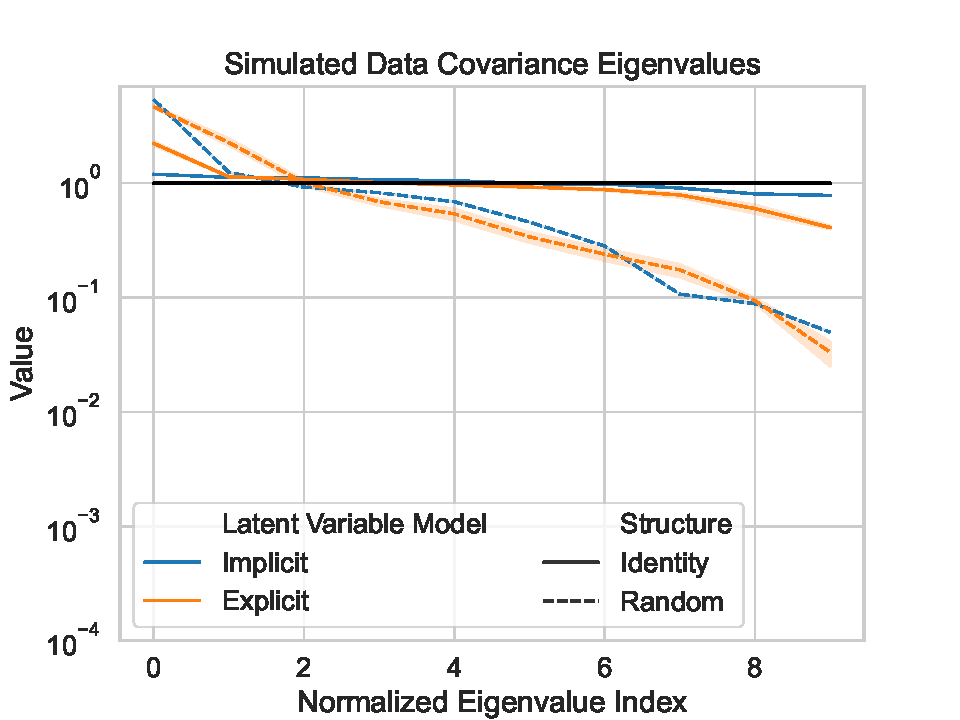
\includegraphics[width=0.8\linewidth]{figures/regularization/covariance/simulated_covariance_eigenvalues_low}
\caption{Eigenvalues of the covariance matrices for the simulated datasets.}\label{fig:covariance-eigenvalues-simulated-low}
\end{figure}

\subsection{High-Dimensional Simulated Data}
In this section we consider only the latent variable models in order to ensure we have a sufficient signal-to-noise ratio to compare the models as we are deliberately undersampled.
Figure~\ref{fig:latent-variable-weights-loadings-high}a once again shows that PCA is a useful baseline for multiview data under an isotropic noise model, even in the high-dimensional setting.
On the other hand, CCA cannot recover any signal when it is overparameterized.
Ridge CCA and PLS perform similarly, perhaps because the only identifiable signal is the PLS signal (since the CCA signal is not identifiable).
Figure~\ref{fig:latent-variable-weights-loadings-high}b illustrates clearly that both RCCA and ElasticNet with their tunable L2 regularization both outperform PLS and SPLS with fixed and maximal L2 regularization.
It appears that in high dimensions correlated noise is a significant problem for PLS (and therefore SPLS) when used as regularized CCA models, even though the models are identifiable.

\begin{figure}
\centering
\begin{subfigure}{0.49\linewidth}
\centering
\includesvg[width=\linewidth]{figures/regularization/simulated/high/Combined_Weights_Loadings_with_Error_Bars_Identity_Covariance_latent_variable}
\caption{Identity Covariance Latent Variable}
\end{subfigure}
%
\begin{subfigure}{0.49\linewidth}
\centering
\includesvg[width=\linewidth]{figures/regularization/simulated/high/Combined_Weights_Loadings_with_Error_Bars_Random_Covariance_latent_variable}
\caption{Random Covariance Latent Variable}
\end{subfigure}
\caption{Weights and Loadings for High-Dimensional Explicit Latent Variable Data Generation.}\label{fig:latent-variable-weights-loadings-high}
\end{figure}

\begin{figure}
\centering
\begin{subfigure}{0.49\linewidth}
\centering
\includesvg[width=\linewidth]{figures/regularization/simulated/high/Train_Test_Scores_Identity_Covariance_latent_variable.svg}
\caption{}
\end{subfigure}
%
\begin{subfigure}{0.49\linewidth}
\centering
\includesvg[width=\linewidth]{figures/regularization/simulated/high/Train_Test_Scores_Random_Covariance_latent_variable.svg}
\caption{}
\end{subfigure}
\caption{Test Scores for High-Dimensional Explicit Latent Variable Data Generation Models.}\label{fig:latent-variable-scores-high}
\end{figure}

%\paragraph{Identitiness of the Covariance Matrices}
%
%As in the low-dimensional case, we can measure the identitiness of the covariance matrices by looking at the eigenvalues of the covariance matrices.
%
%\begin{figure}
%\centering
%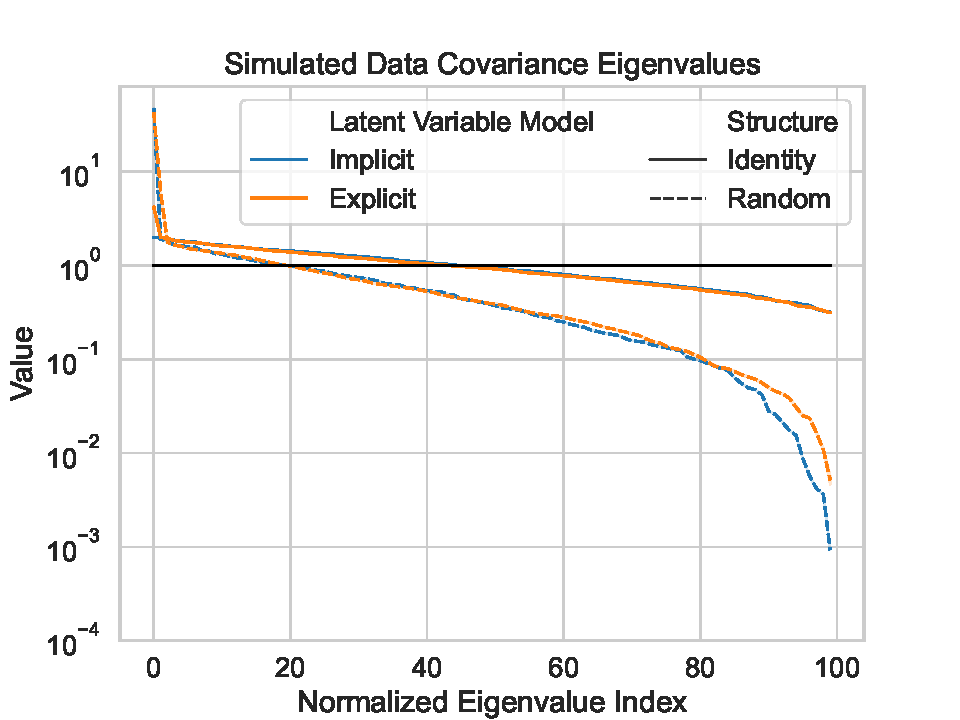
\includegraphics[width=0.8\linewidth]{figures/regularization/covariance/simulated_covariance_eigenvalues_high}
%\caption{Eigenvalues of the covariance matrices for the simulated datasets.}\label{fig:covariance-eigenvalues-simulated-high}
%\end{figure}

\newpage
\subsection{Human Connectome Project (HCP) Data}

Next, we consider the results of applying the various CCA variants to the HCP data.
Since the HCP data is high-dimensional, we drop CCA from the analysis since it would produce random results.

\subsubsection{Out of Sample Correlation}

The Elastic Net did not improve upon Ridge CCA in terms of holdout correlation captured (Figure~\ref{fig:performance}).
However, both Ridge CCA and ElasticNet outperformed PLS and SPLS.
This suggests that tunable L2 regularization is important, even for very high-dimensional data.
SPLS does however outperform PLS.

\begin{figure}
\centering
\includegraphics[width=0.5\linewidth]{figures/regularization/hcp/holdout_correlations}
\caption{Out-of-sample canonical correlations for each model.}
\end{figure}

\subsubsection{Behaviour Weights and Loadings}

Figure\ref{fig:behaviour} plots the top 8 positive and negative non-imaging loadings and their associated weights for each model\footnote{This can and does mean for example that a zero weight may have a non-zero loading!}.
This is to illustrate some of the effects we have observed in the previous section.
PCA finds a mode of variation in the behavioural data that is positively correlated with psychiatric and life function tests and negatively correlated with a number of emotion and personality tests.
The RCCA and ElasticNet models find a mode of variation in the behavioural data that is negatively correlated with the Line Orientation test and to a lesser extent smoking and positively correlated with a number of other cognitive tests.
The PLS model finds a mode of variation in the behavioural data that is somewhat similar to the `good-bad' mode in\cite{smith2015positive} with a positive correlation with agreeableness, vocabulary tests, and feelings about ones' life and a strong negative correlation with smoking, rule-breaking, and antisocial personality traits.
The SPLS mode is similar but selects out the rule-breaking and antisocial personality traits in favour of the vocabulary tests and smoking.

\begin{figure}
\centering
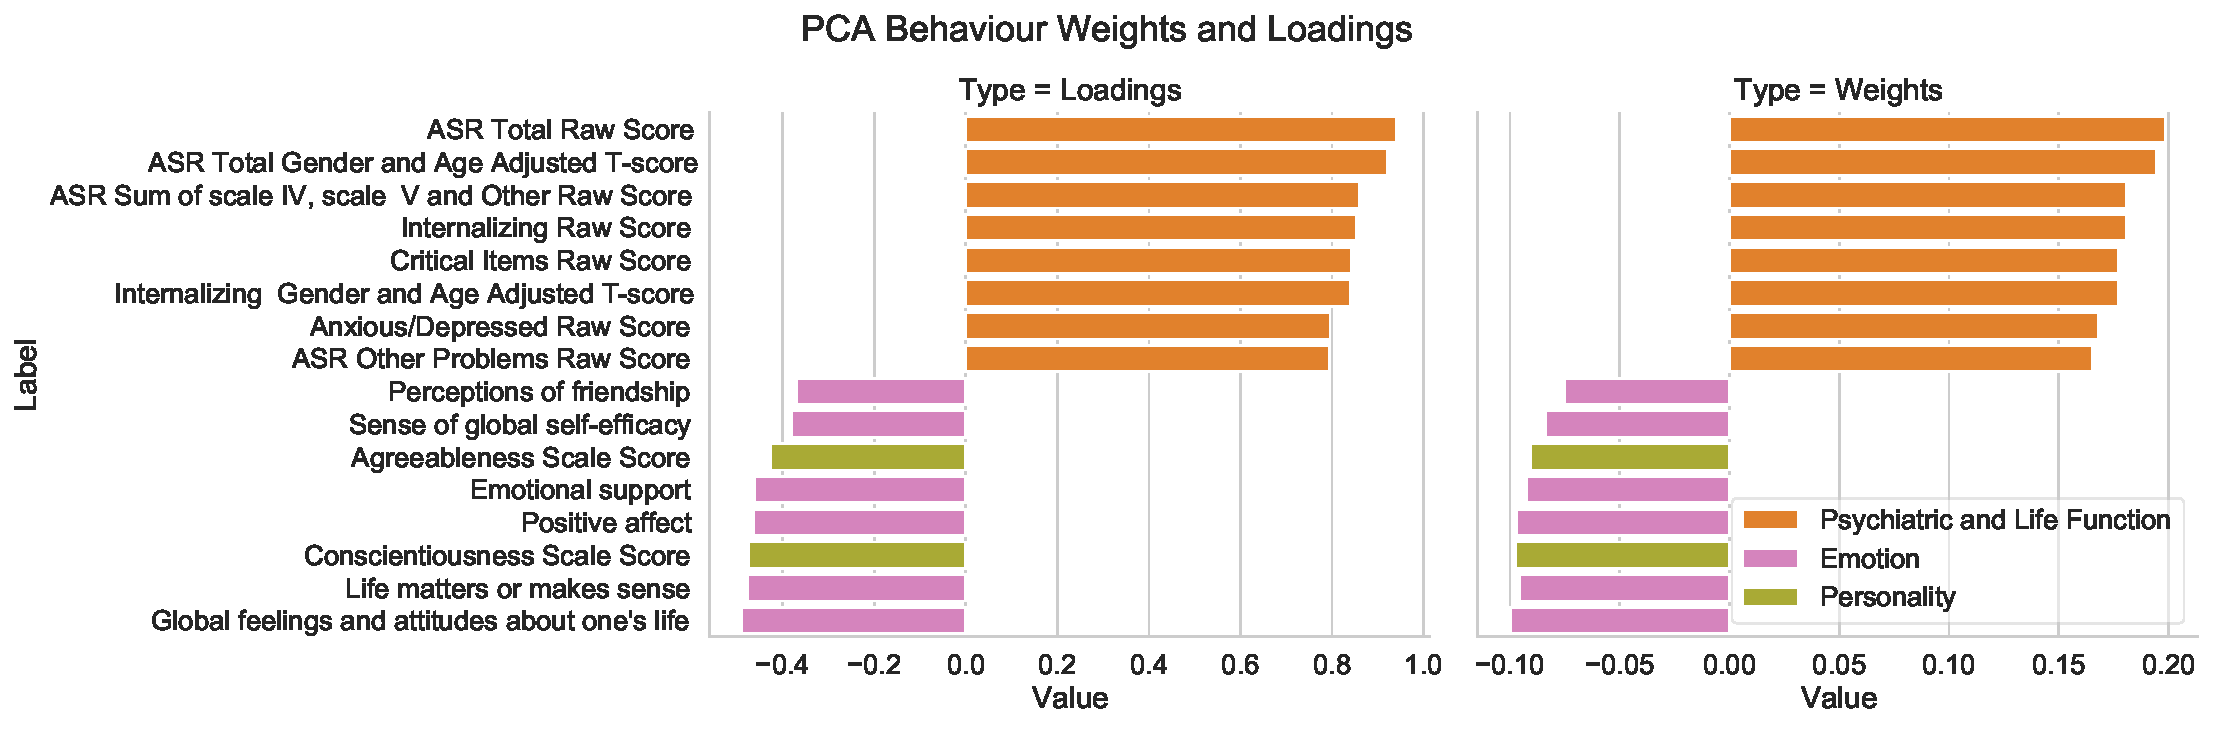
\includegraphics[width=0.8\linewidth]{figures/regularization/hcp/PCA behaviour weights and loadings}
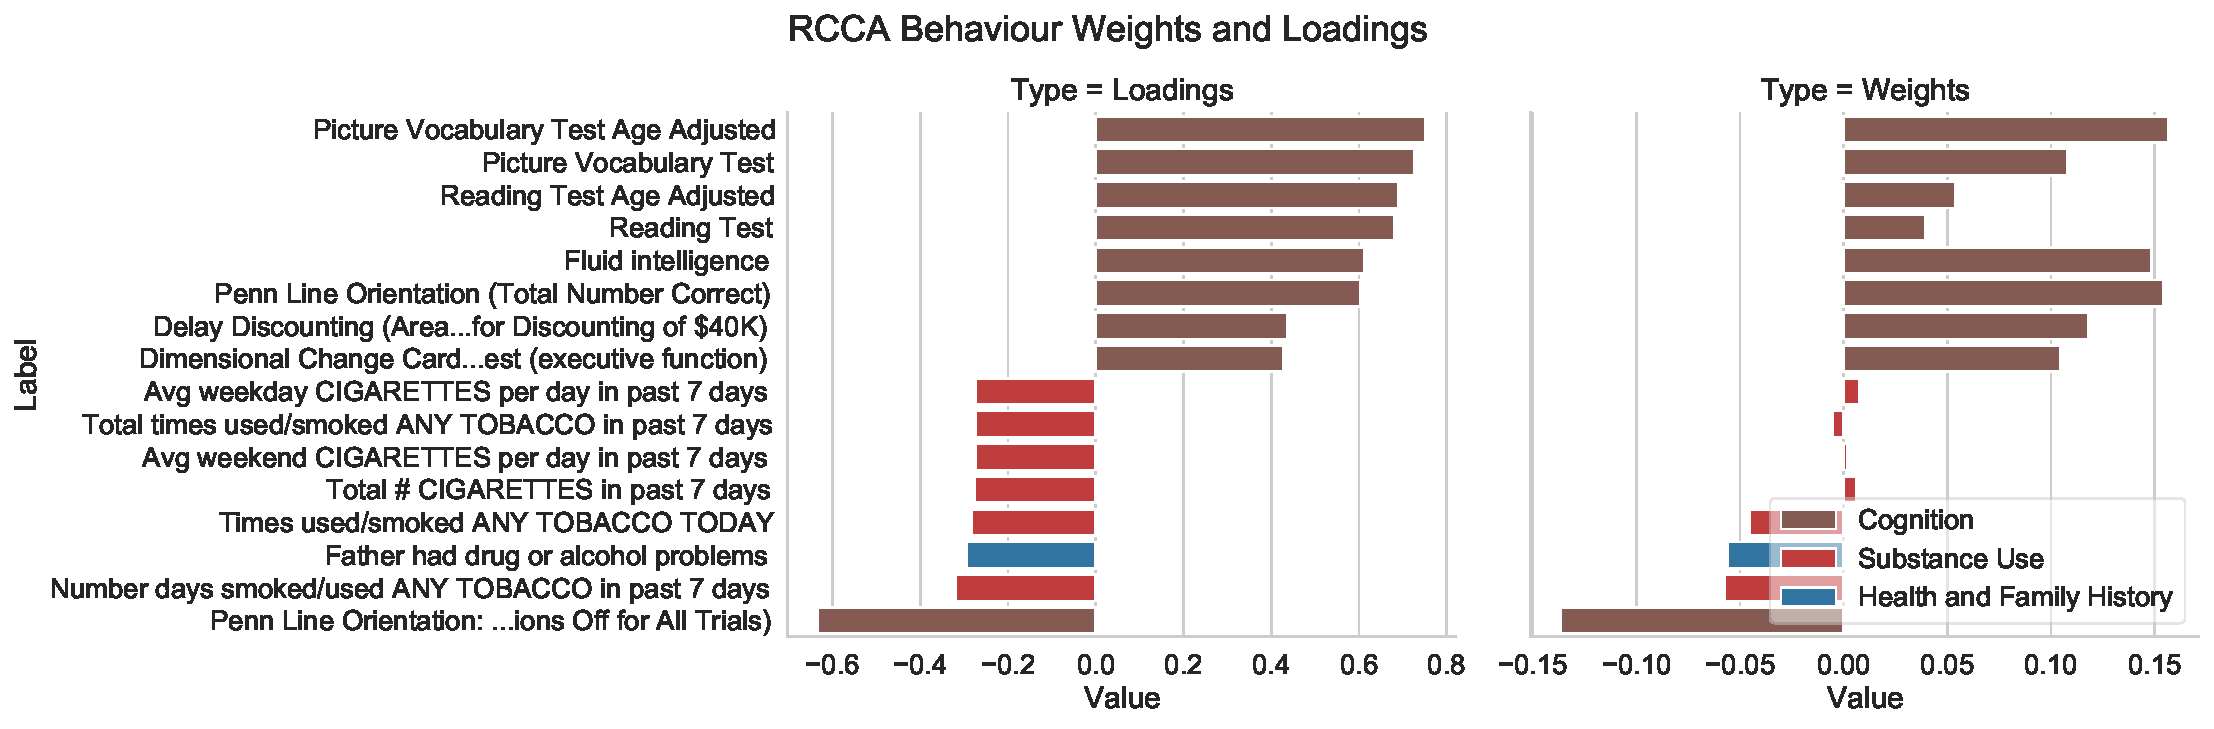
\includegraphics[width=0.8\linewidth]{figures/regularization/hcp/RCCA behaviour weights and loadings}
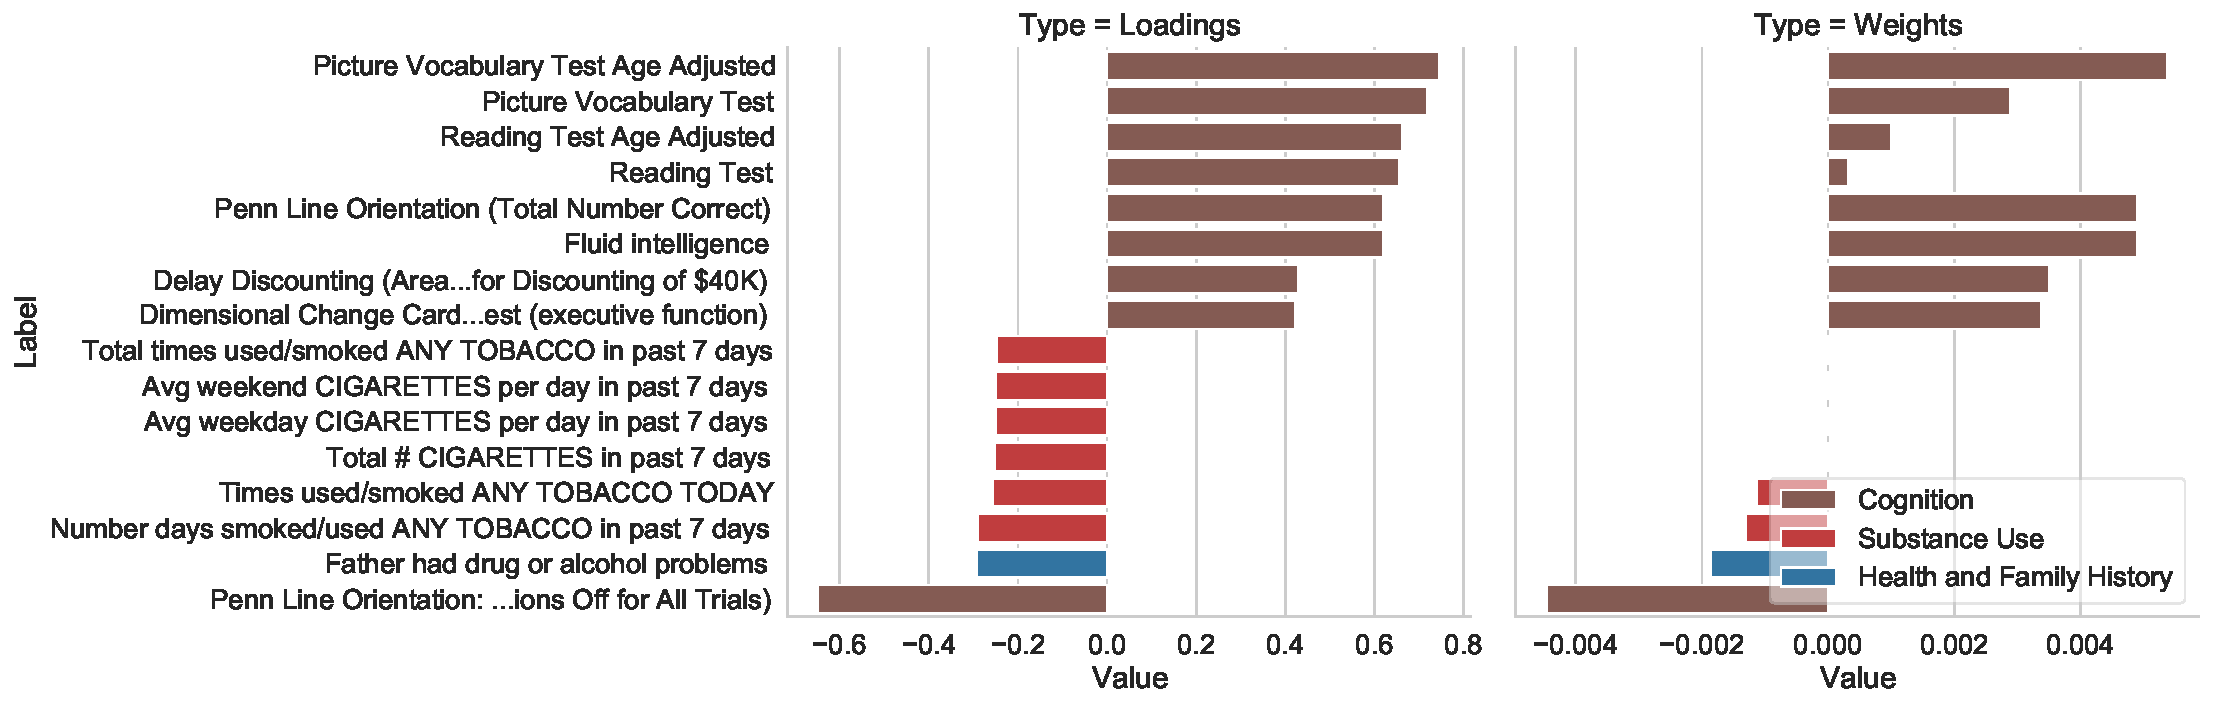
\includegraphics[width=0.8\linewidth]{figures/regularization/hcp/ElasticNet behaviour weights and loadings}
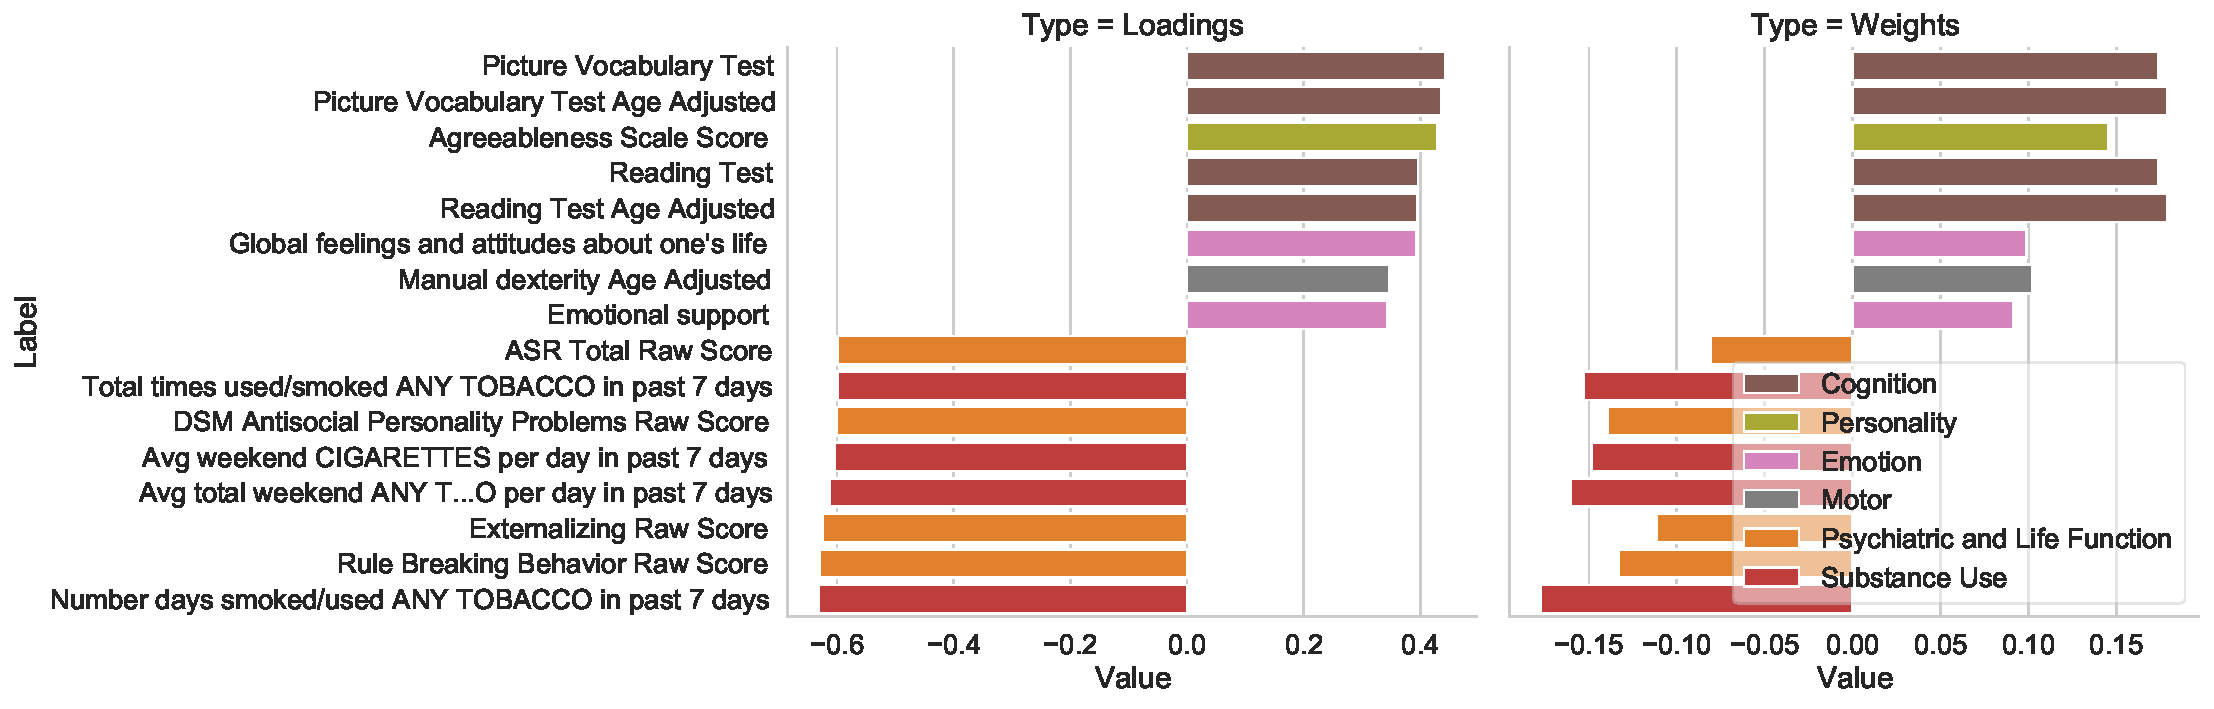
\includegraphics[width=0.8\linewidth]{figures/regularization/hcp/PLS behaviour weights and loadings}
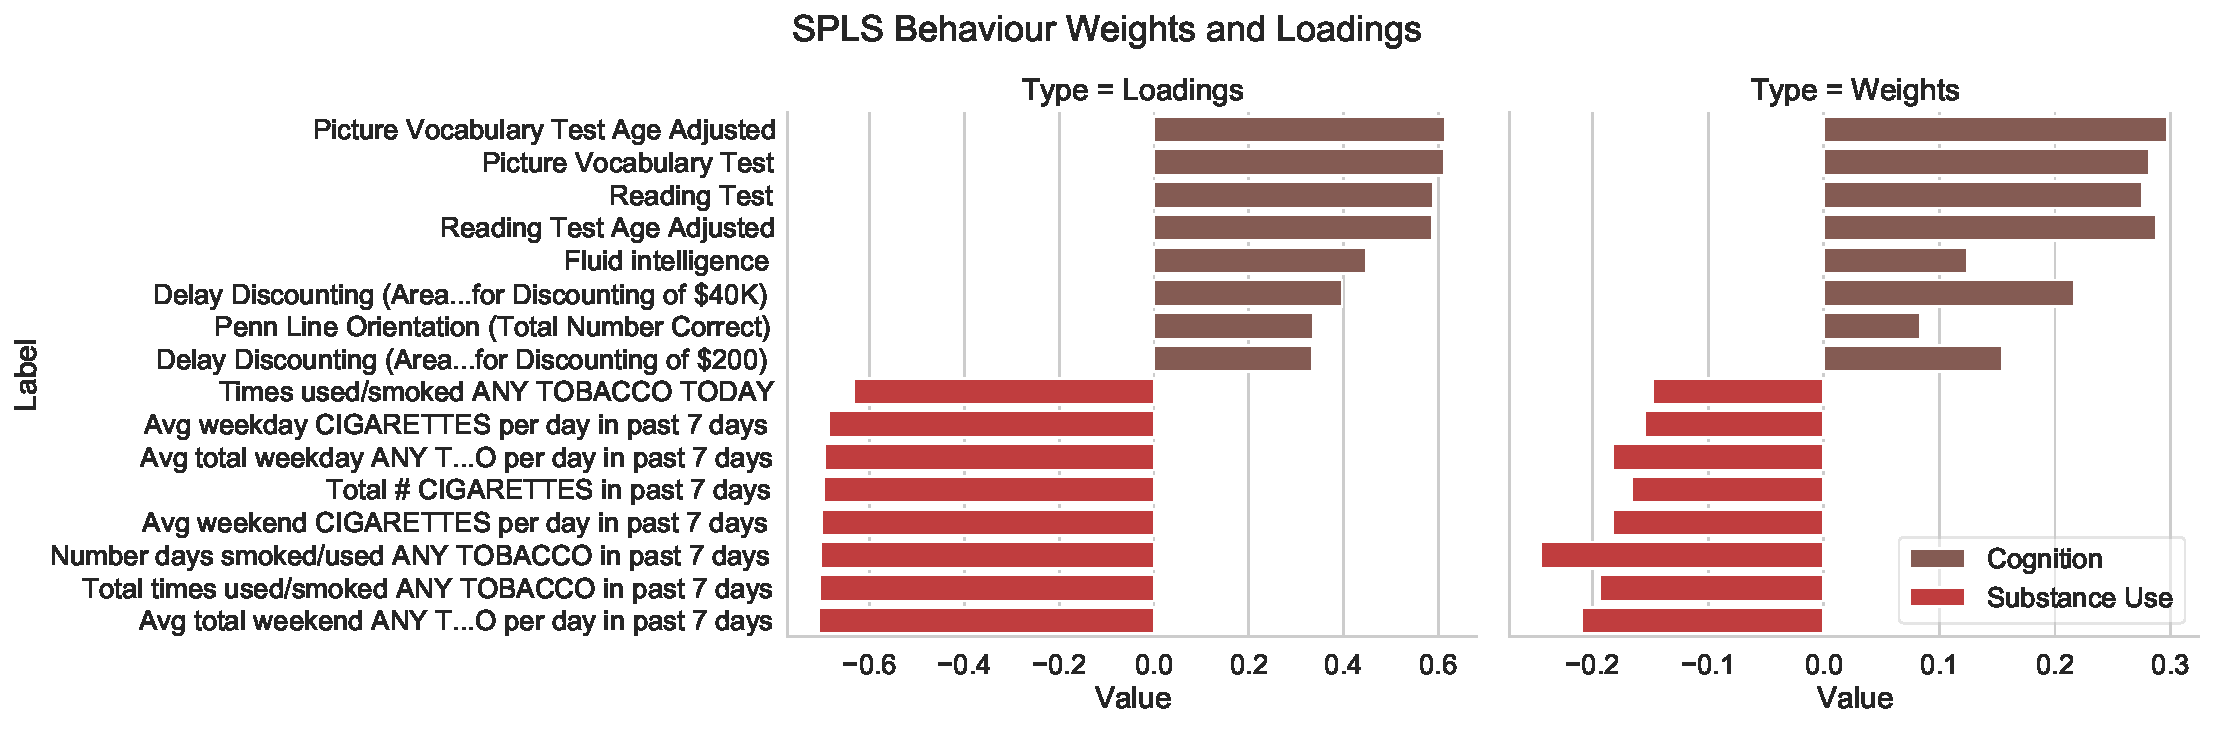
\includegraphics[width=0.8\linewidth]{figures/regularization/hcp/SPLS behaviour weights and loadings}
\caption{Top 8 positive and negative non-imaging loadings for each model}\label{fig:behaviour}
\end{figure}

\subsubsection{Brain Connectivity Weights and Loadings}

In this section, we use two different methods to visualize the brain connectivity weights and loadings.
The first method is to use chord diagrams to visualize the top 8 positive and negative brain weights and loadings for each model.
This approach is inspired by the chord diagrams used in \cite{smith2015positive}.
The second method is to use surface maps to visualize the brain connectivity weights and loadings.
This approach has been used by both \cite{ferreira2022hierarchical} and \cite{smith2015positive}.

\paragraph{Chord Diagrams}
We grouped the nodes of the connectivity matrix of our data into 7 parcels according to the Yeo 7 network parcellation\cite{yeo2011organization}.
These are then arranged around the circumference of the chord diagram using the Nichord package\cite{bogdan2023connsearch}.
The plots then show the 8 strongest positive and negative weights or loadings for each model as `chords'.
The chord diagrams in Figure~\ref{fig:chord_weights} and Figure~\ref{fig:chord_loadings} show the top 8 positive and negative brain weights and loadings for each model.

\textcolor{red} Need to find something biologically useful to say about these.

\begin{figure}
\centering
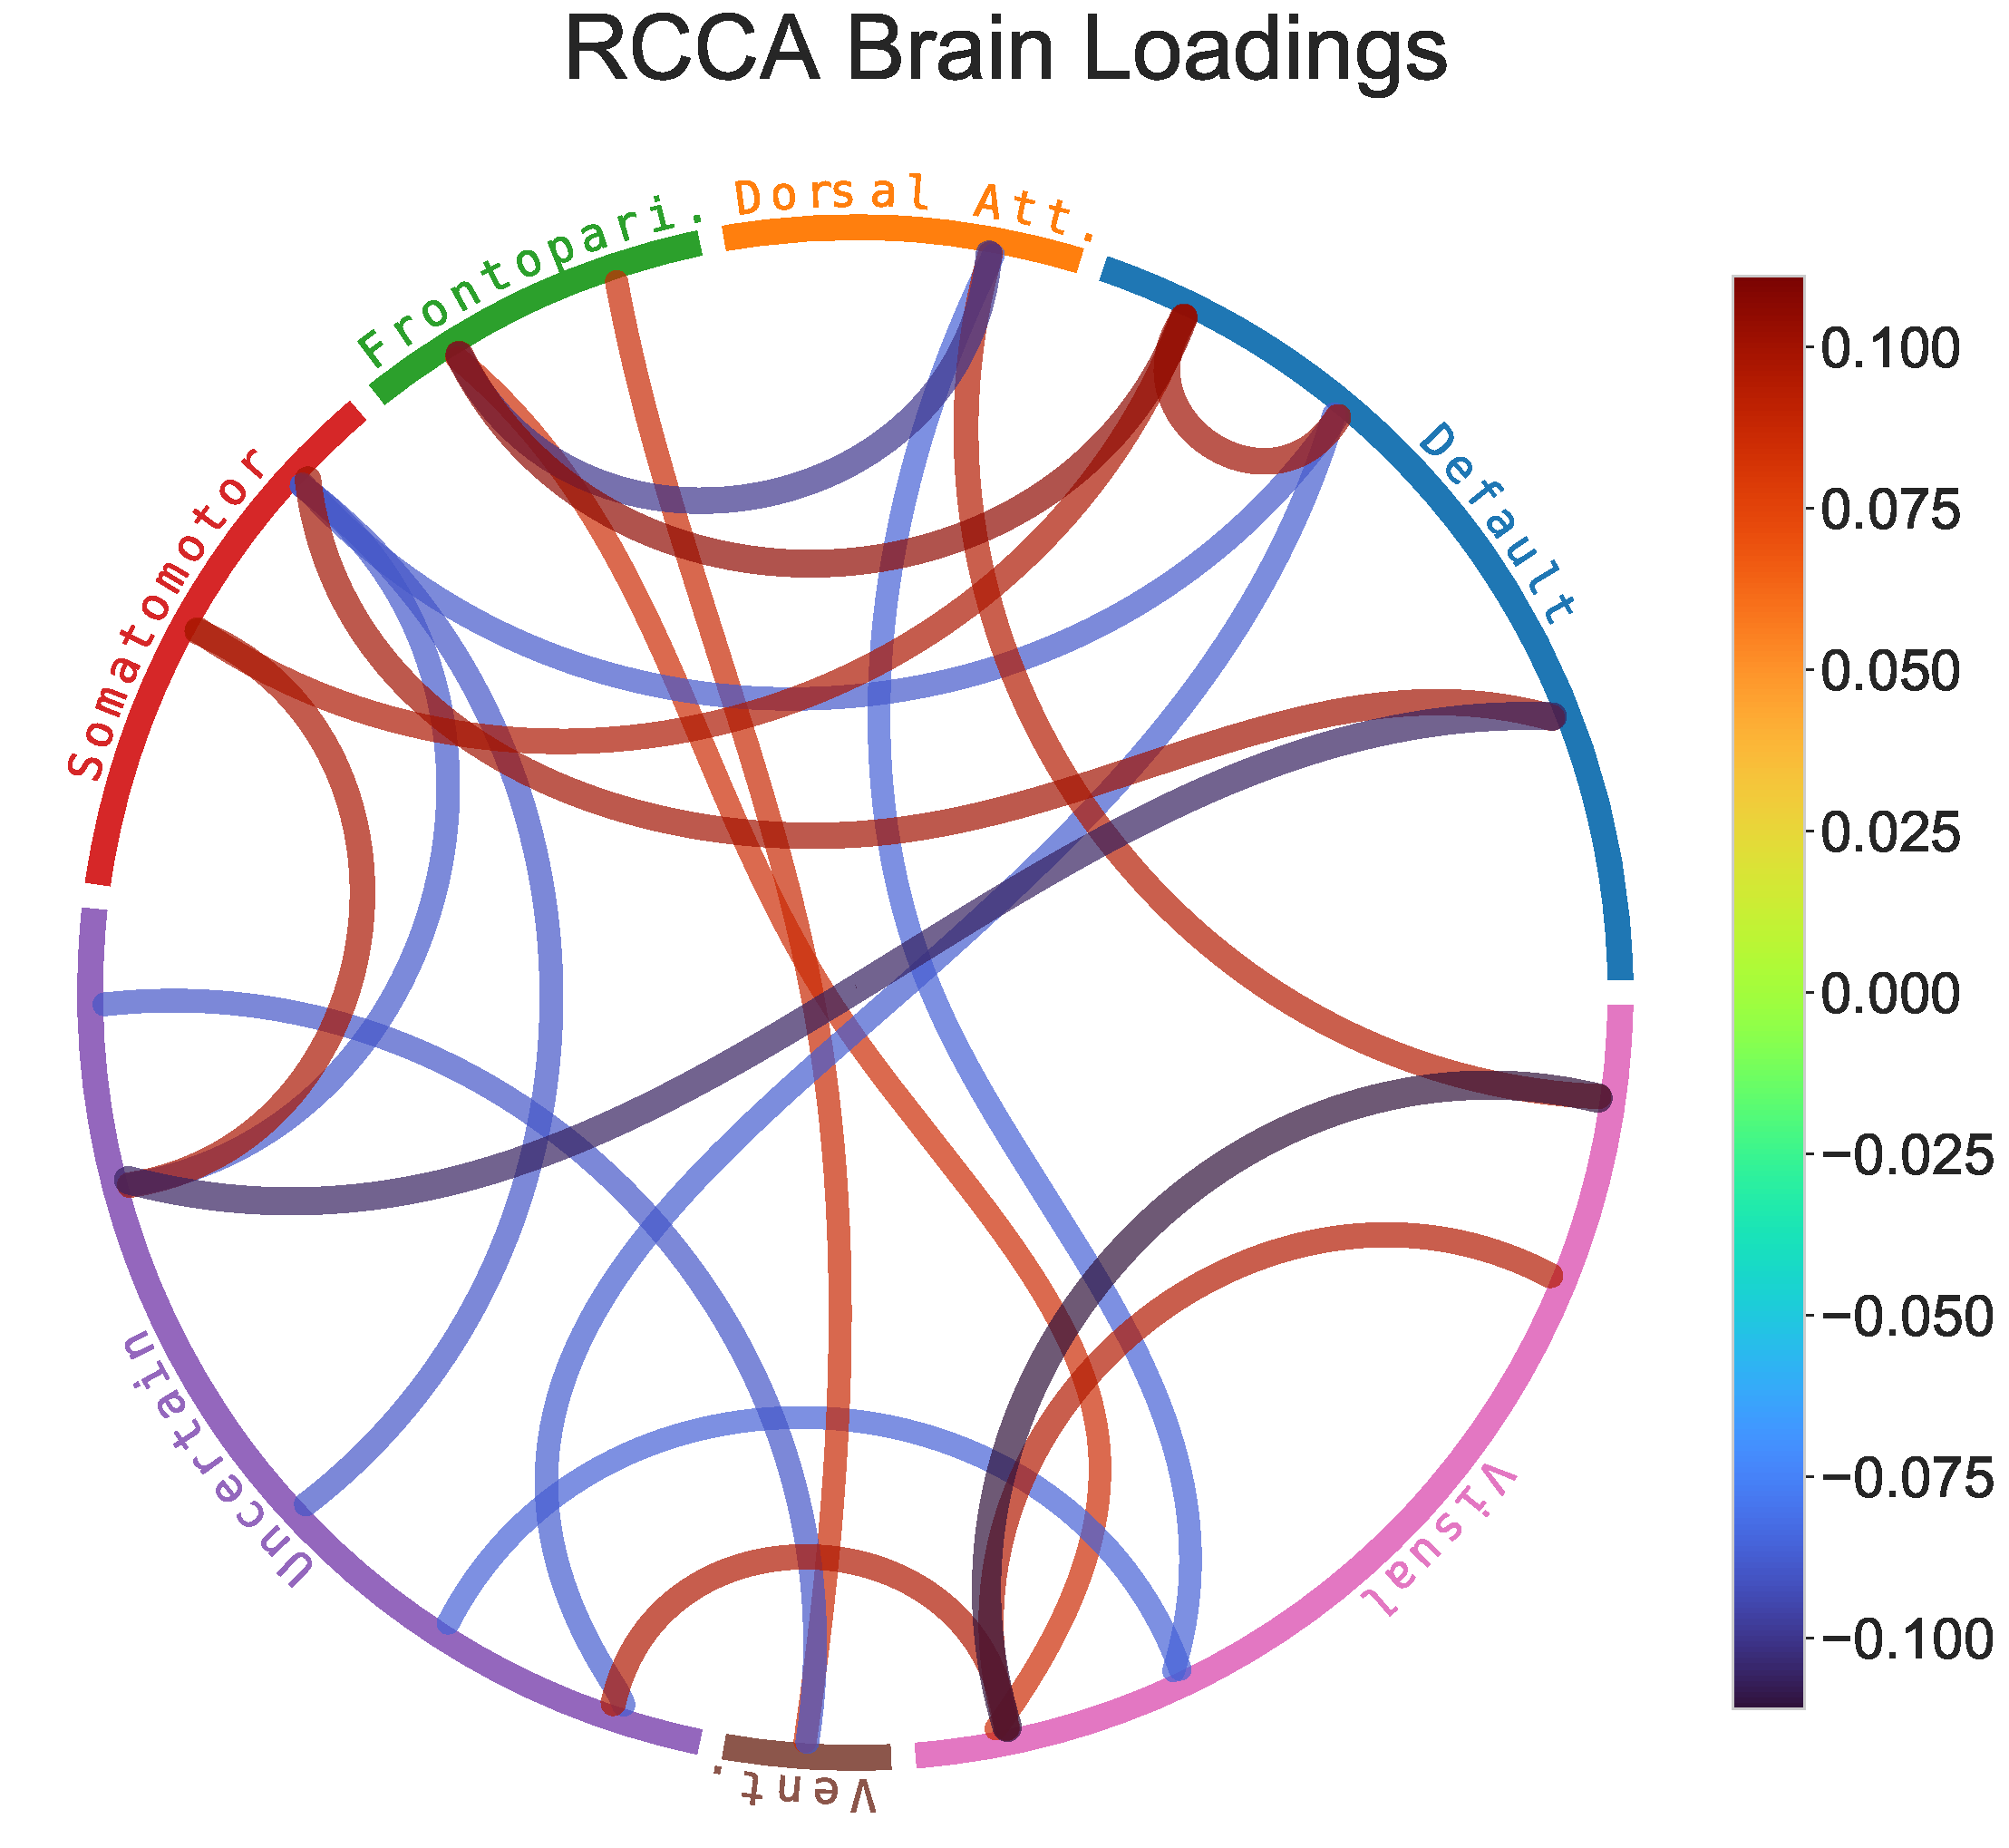
\includegraphics[width=0.49\linewidth]{figures/regularization/hcp/RCCA brain weights}
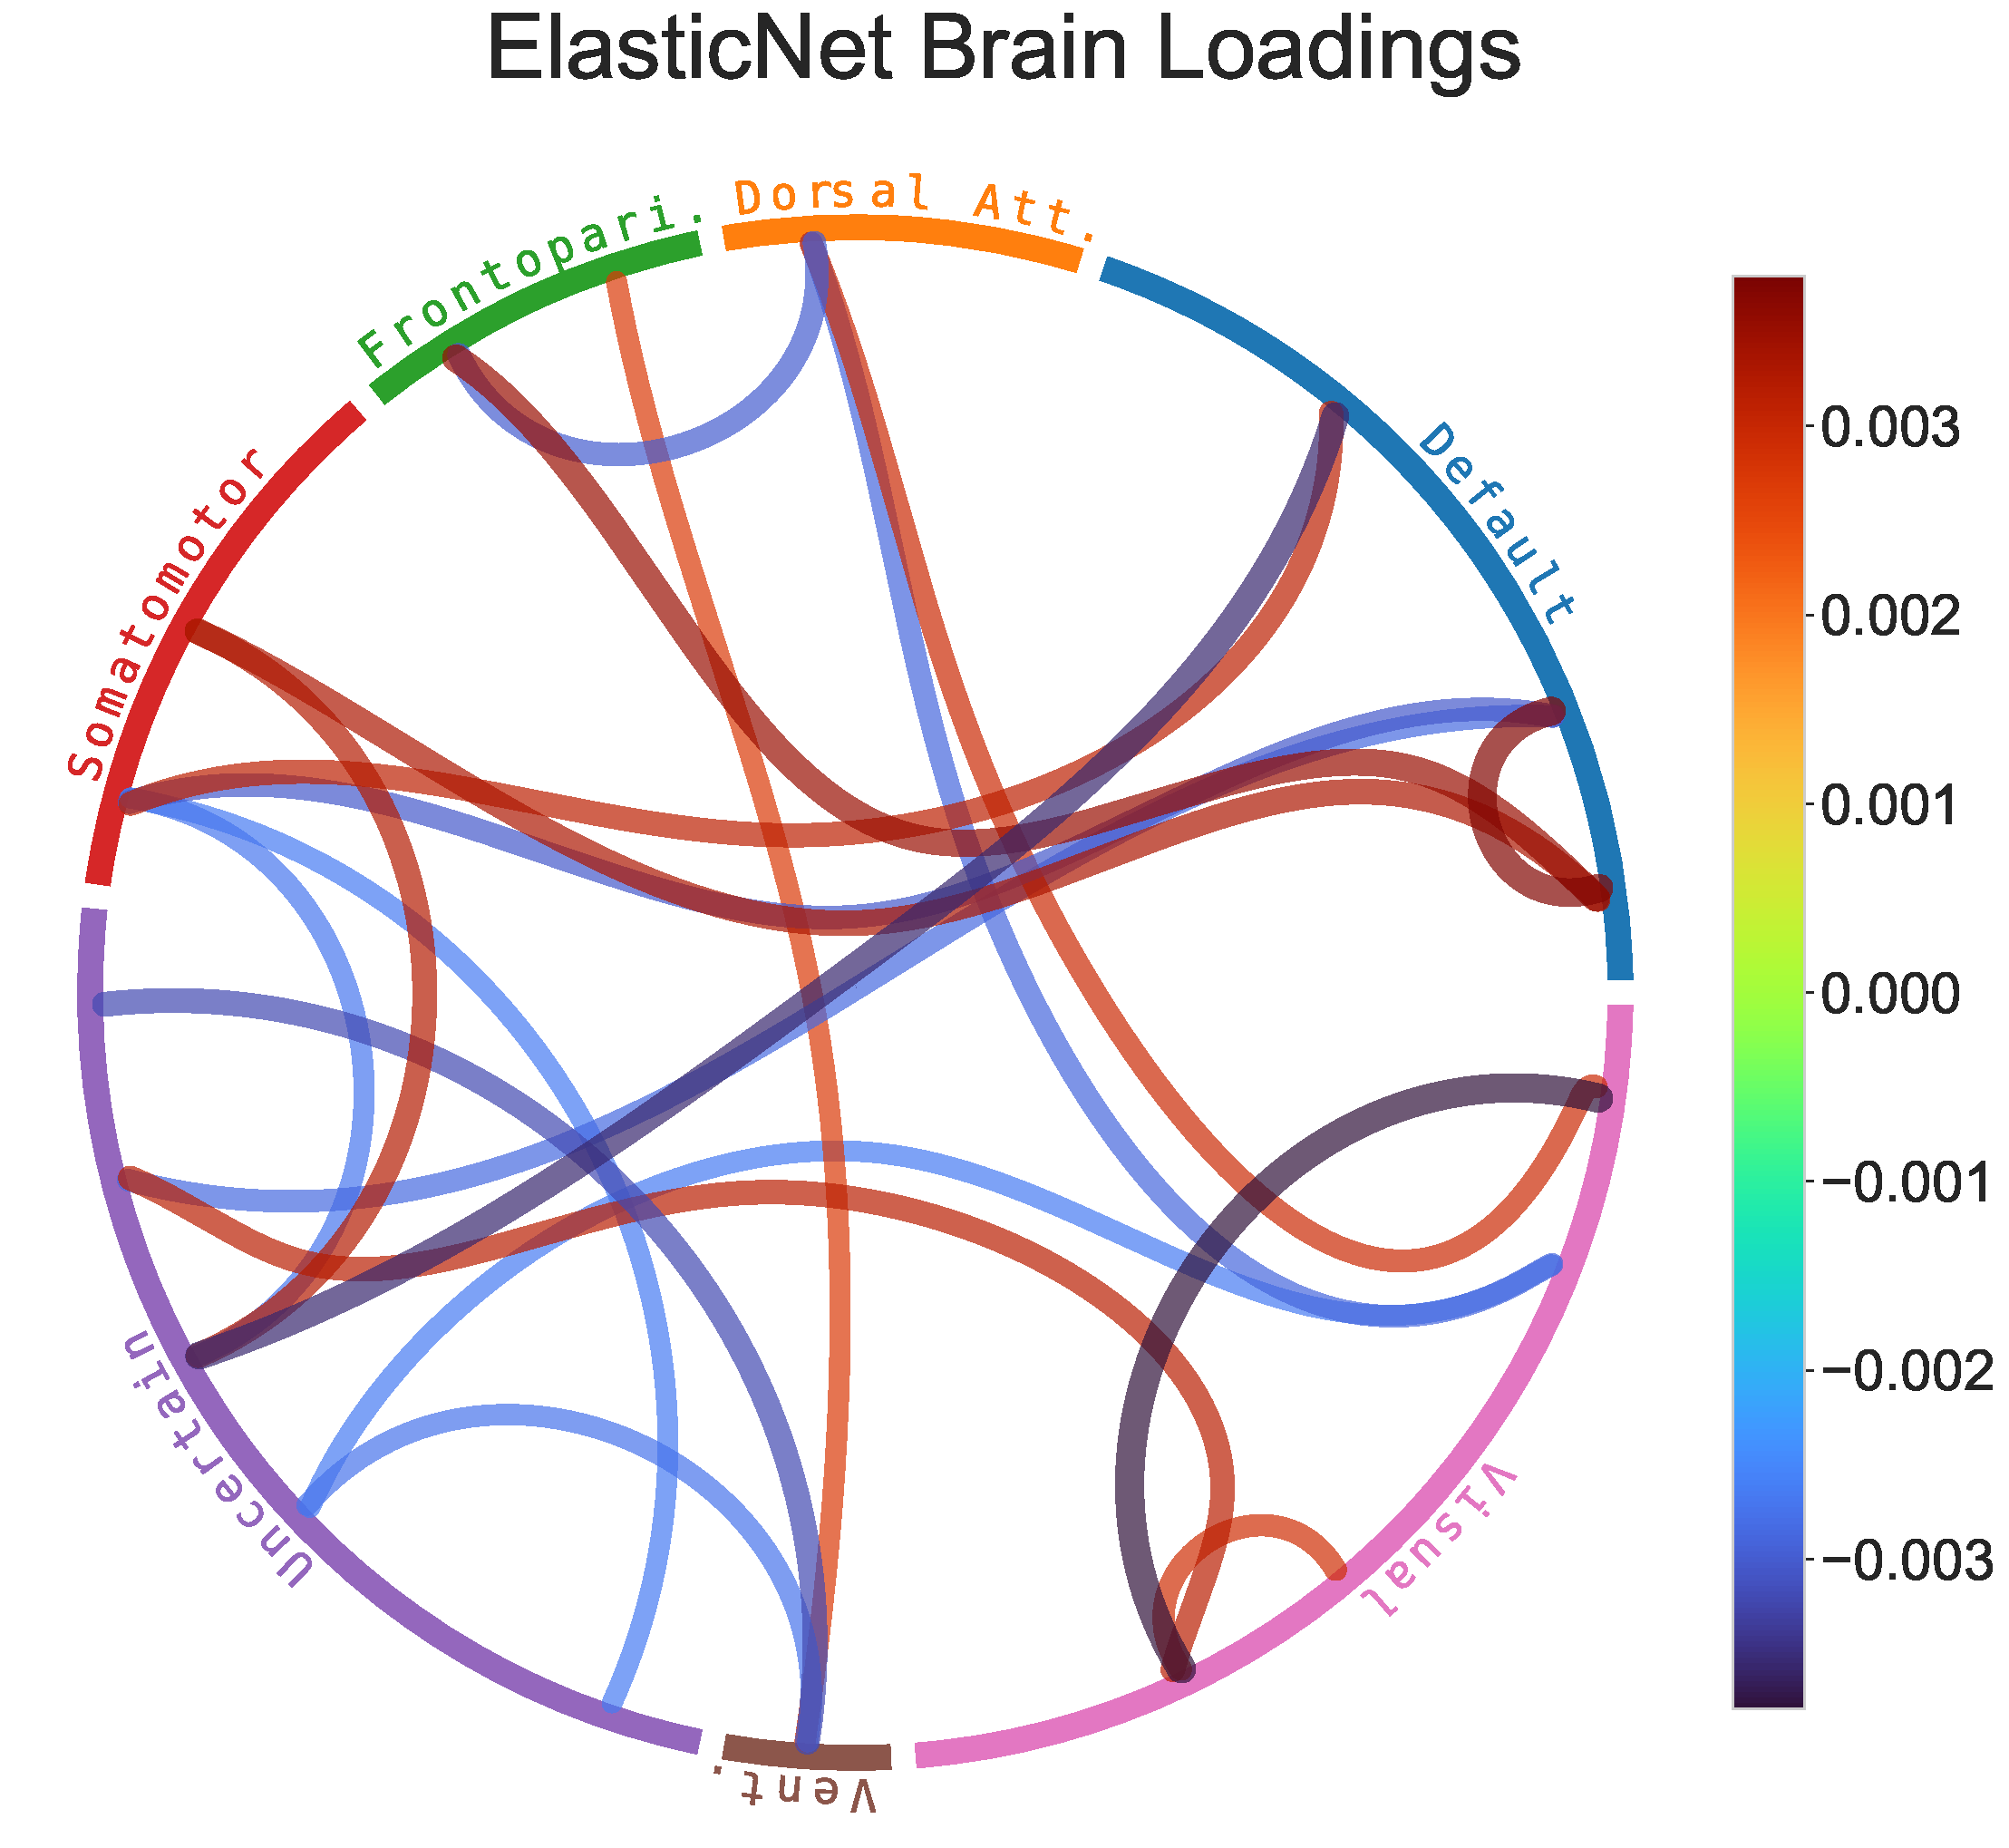
\includegraphics[width=0.49\linewidth]{figures/regularization/hcp/ElasticNet brain weights}
\includegraphics[width=0.49\linewidth]{figures/regularization/hcp/PLS brain weights}
\includegraphics[width=0.49\linewidth]{figures/regularization/hcp/SPLS brain weights}
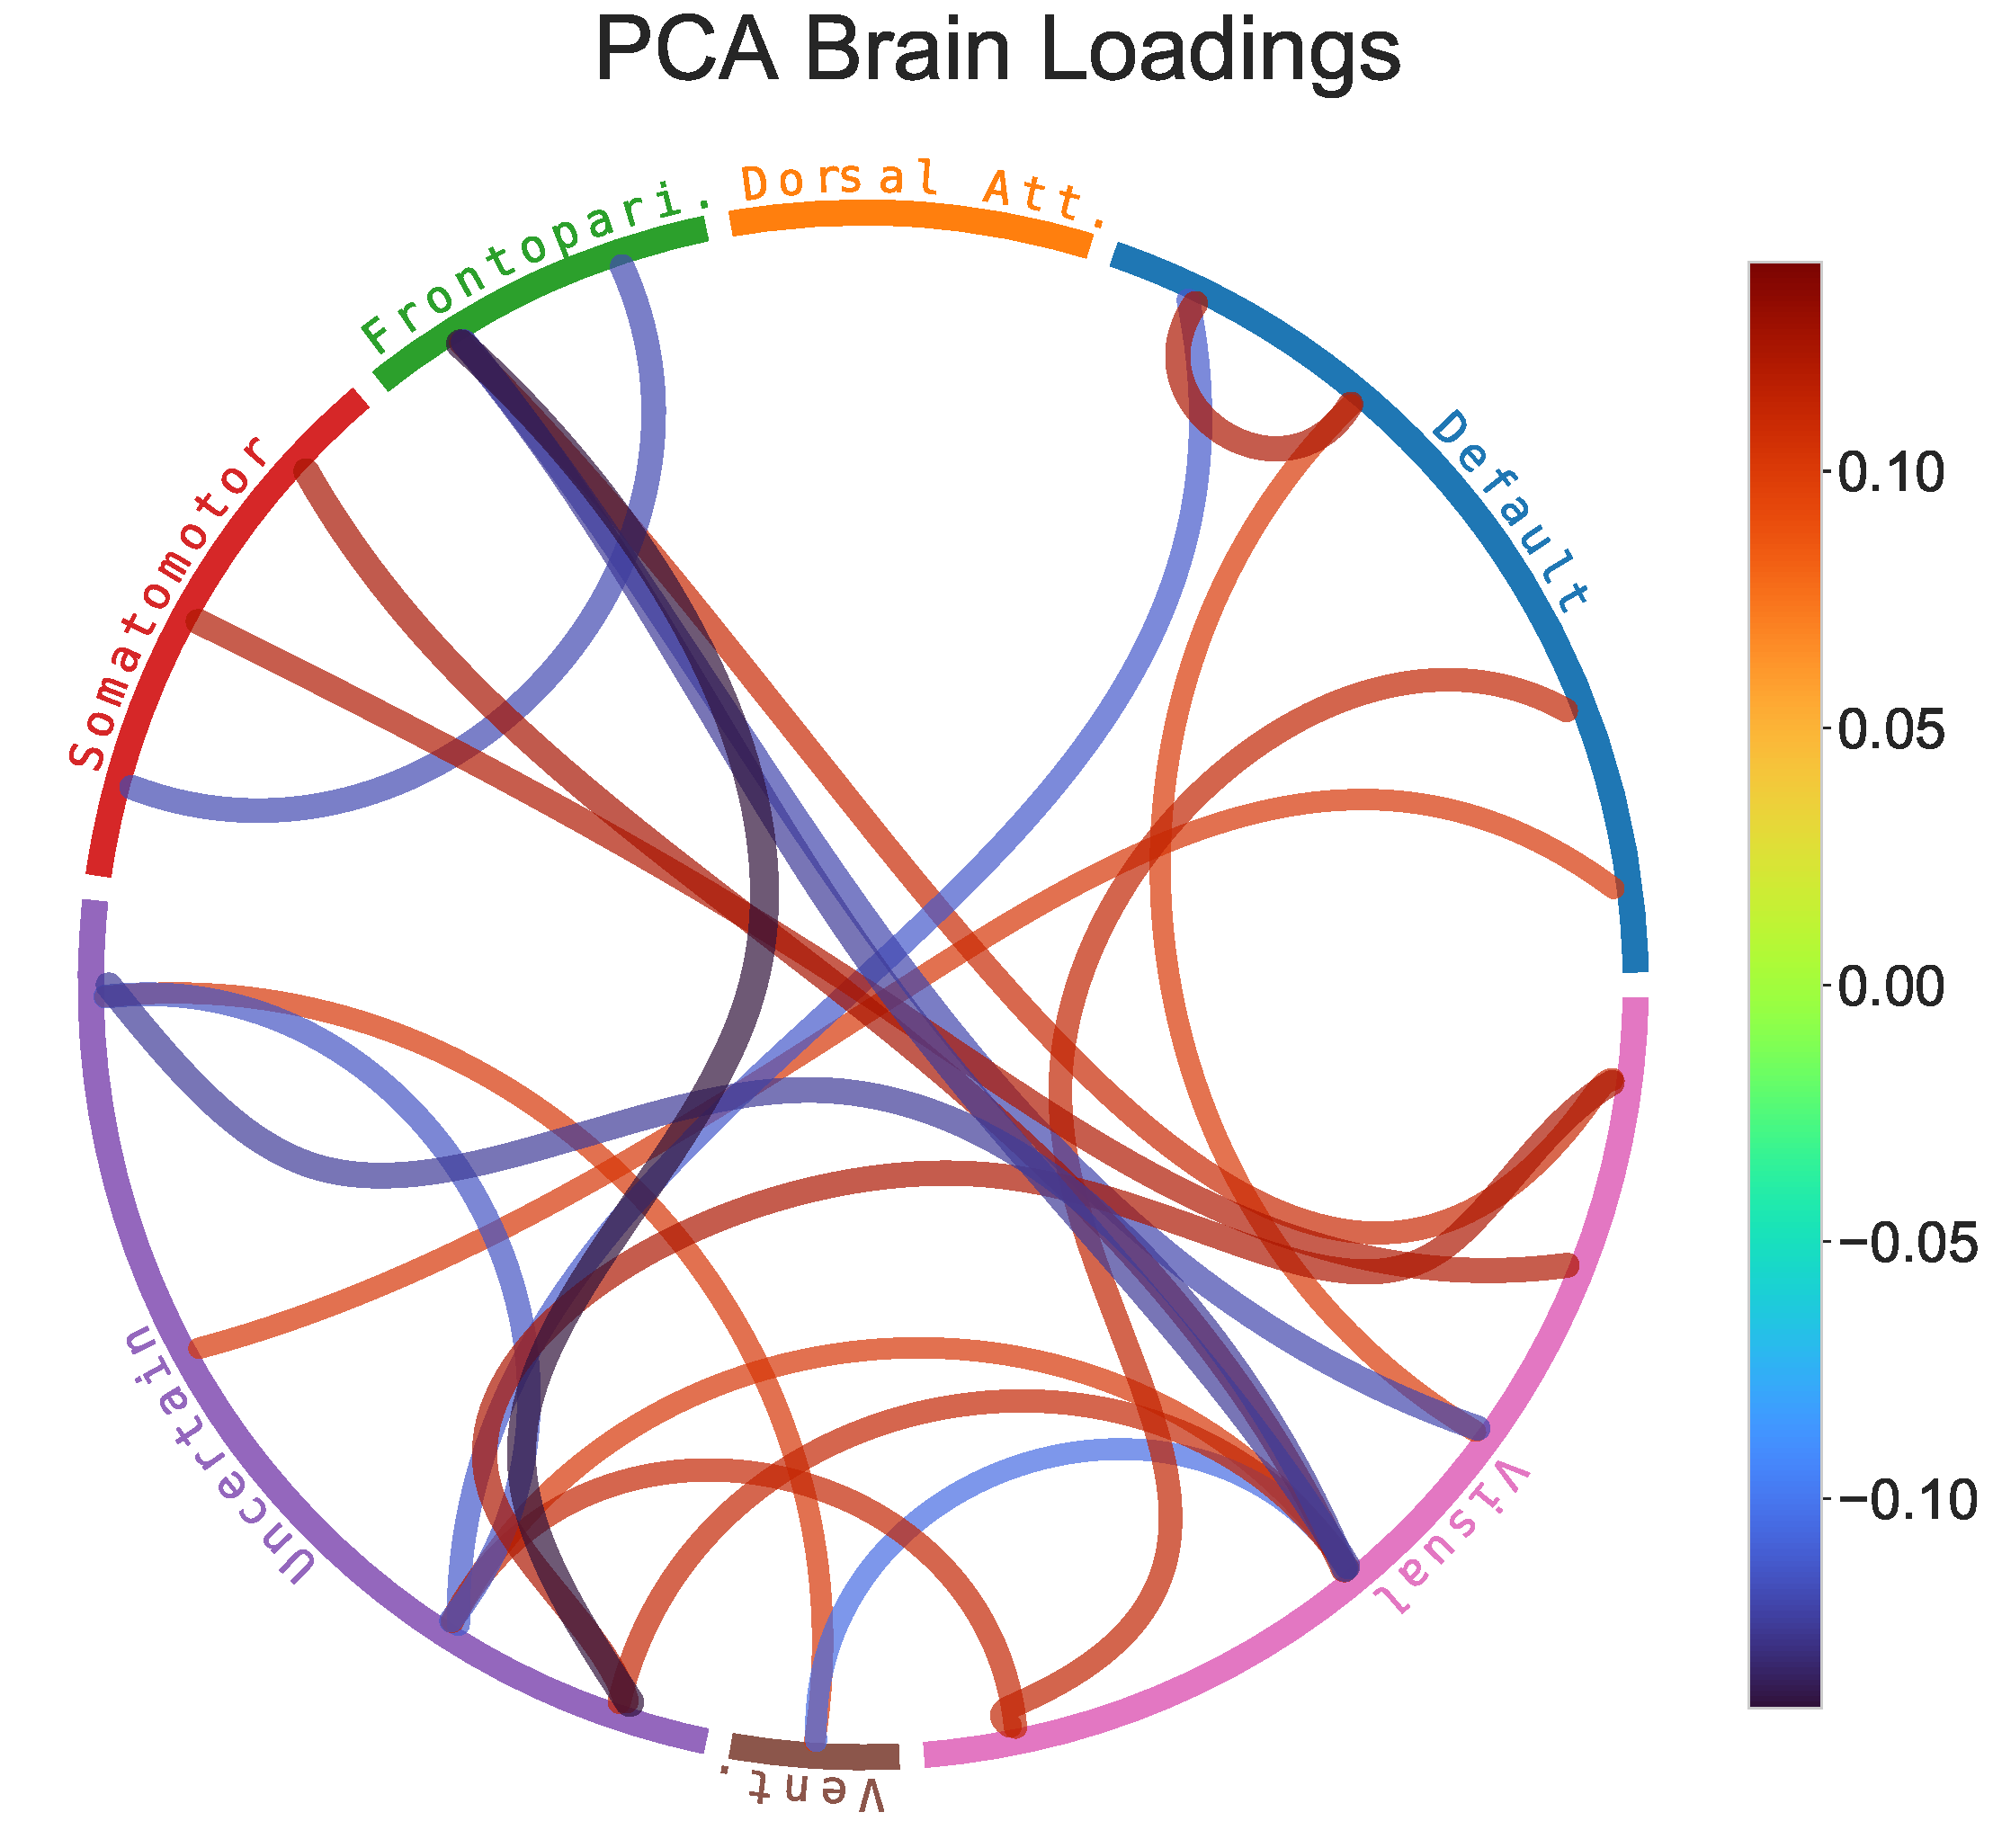
\includegraphics[width=0.49\linewidth]{figures/regularization/hcp/PCA brain weights}
\caption{Chord diagrams of the top 8 positive and negative brain weights for each model.}\label{fig:chord_weights}
\end{figure}

\begin{figure}
\centering
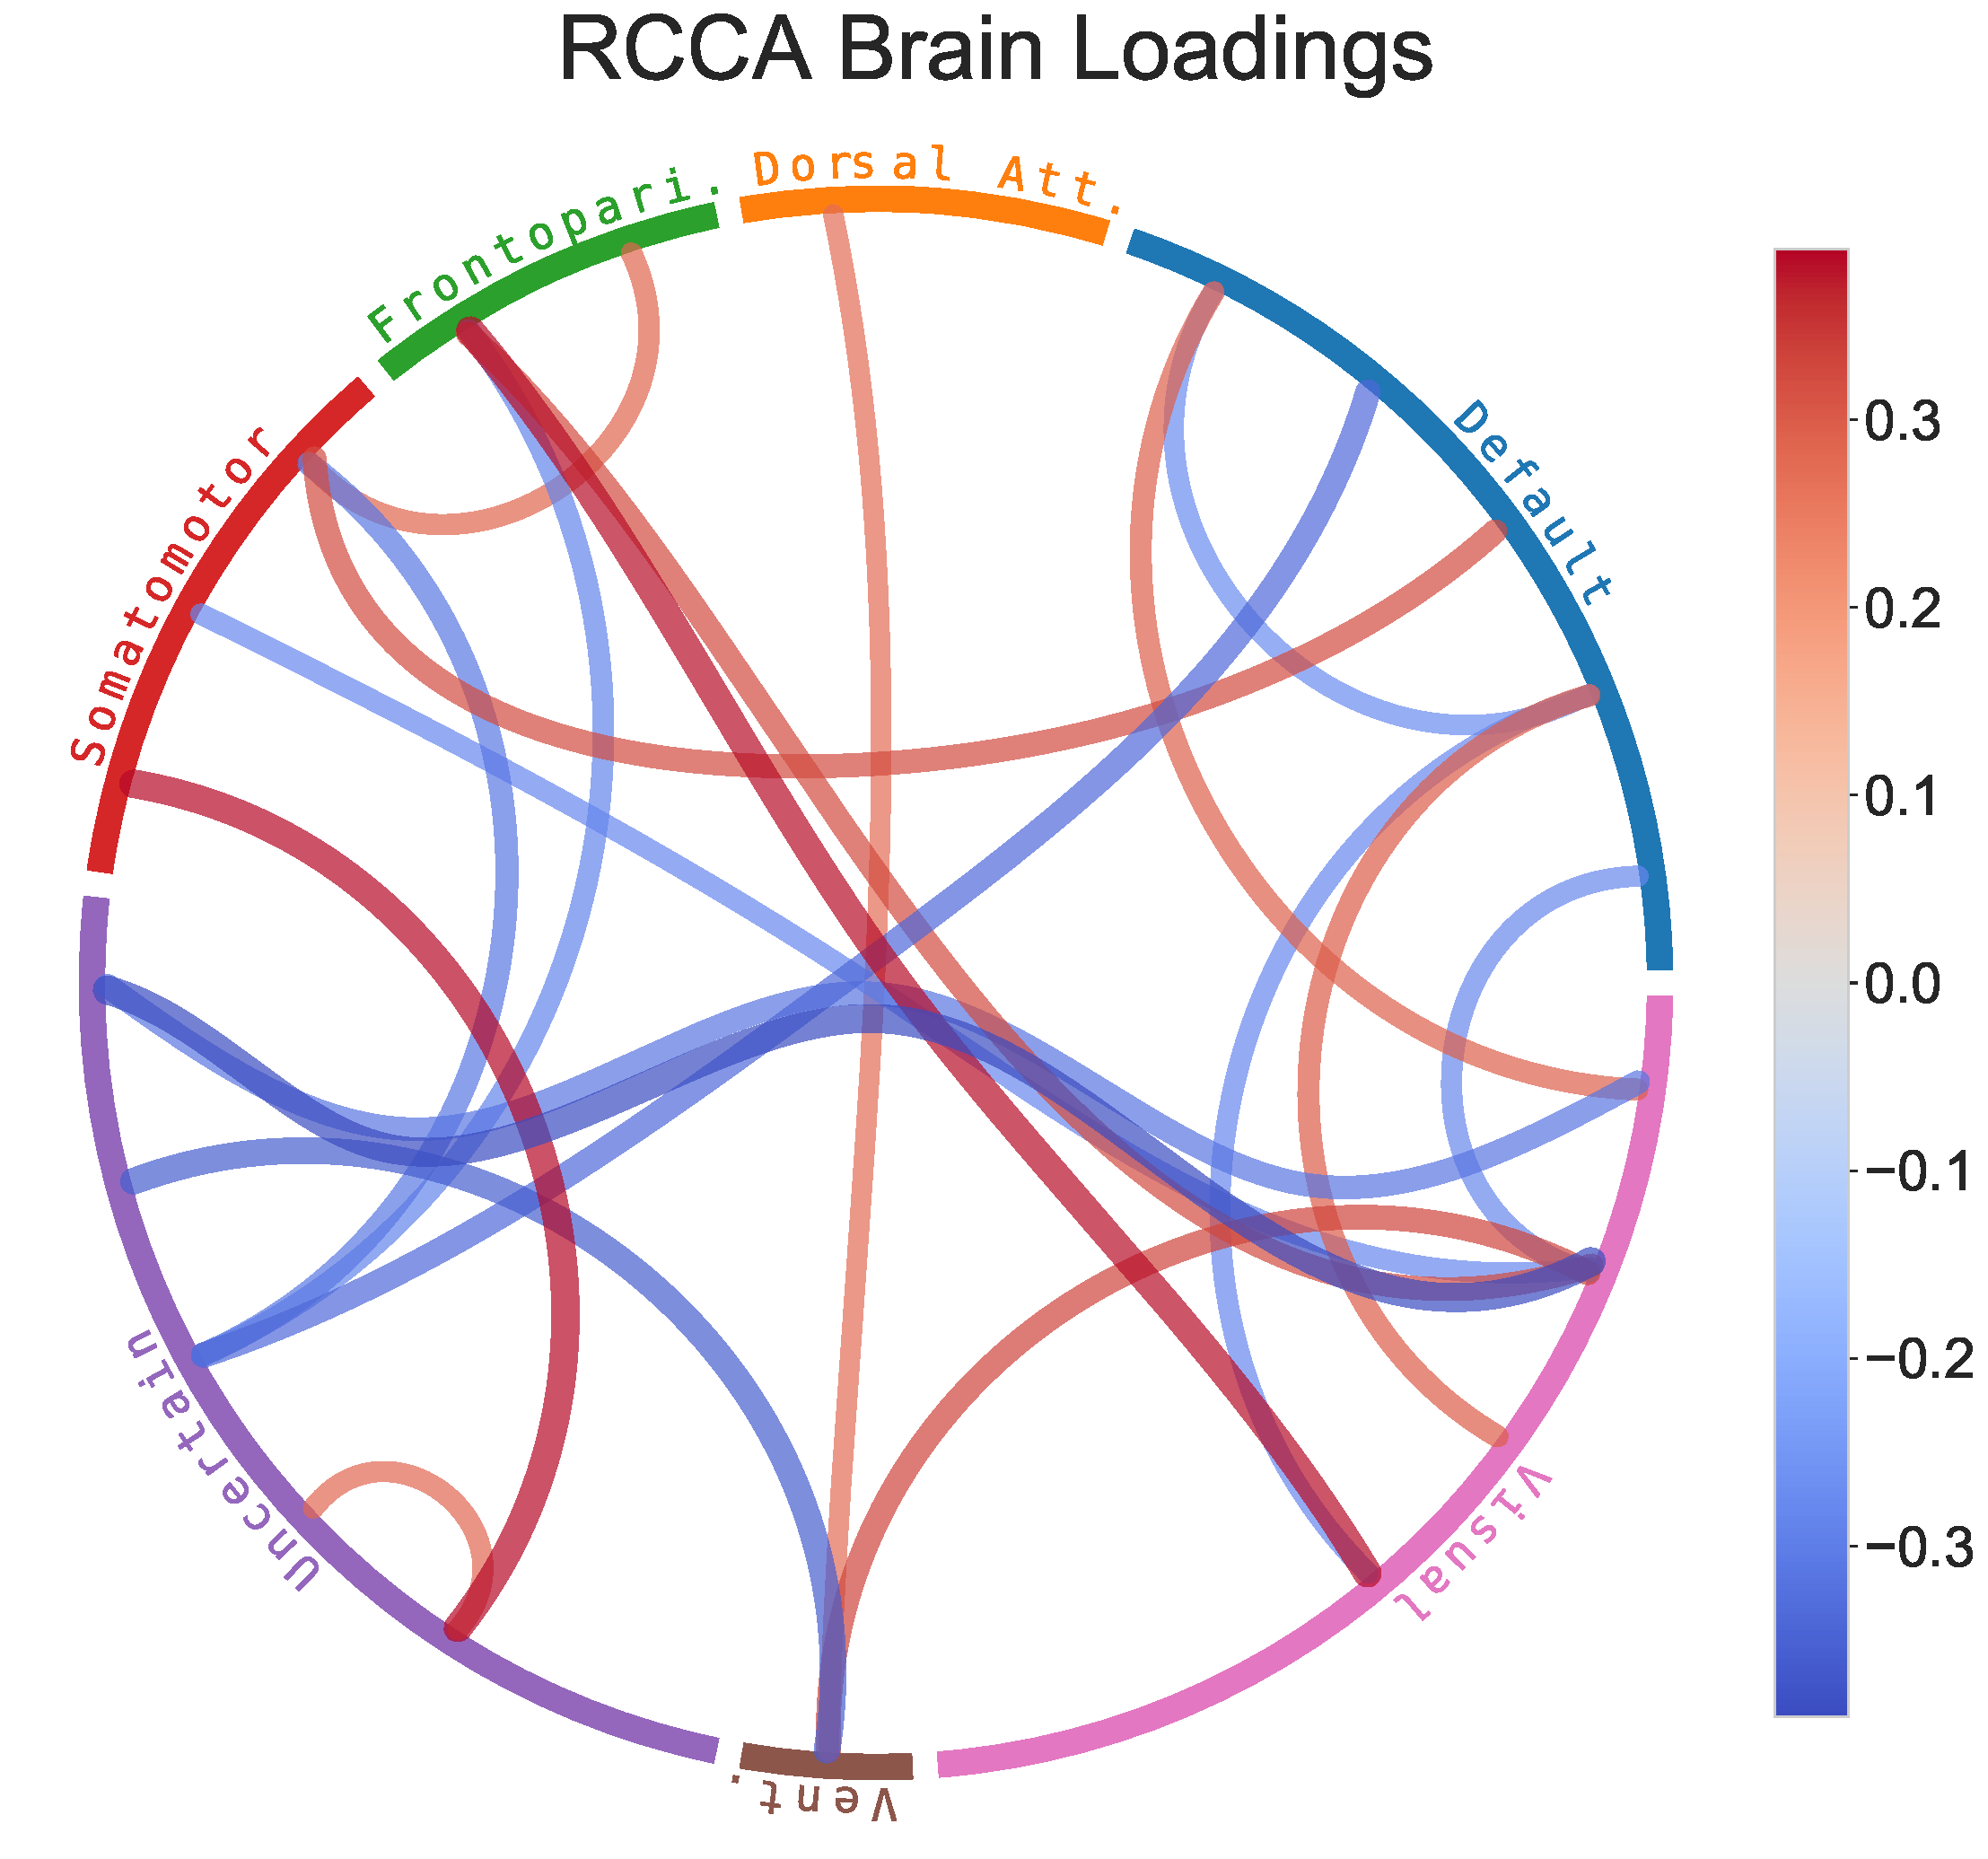
\includegraphics[width=0.49\linewidth]{figures/regularization/hcp/RCCA brain loadings}
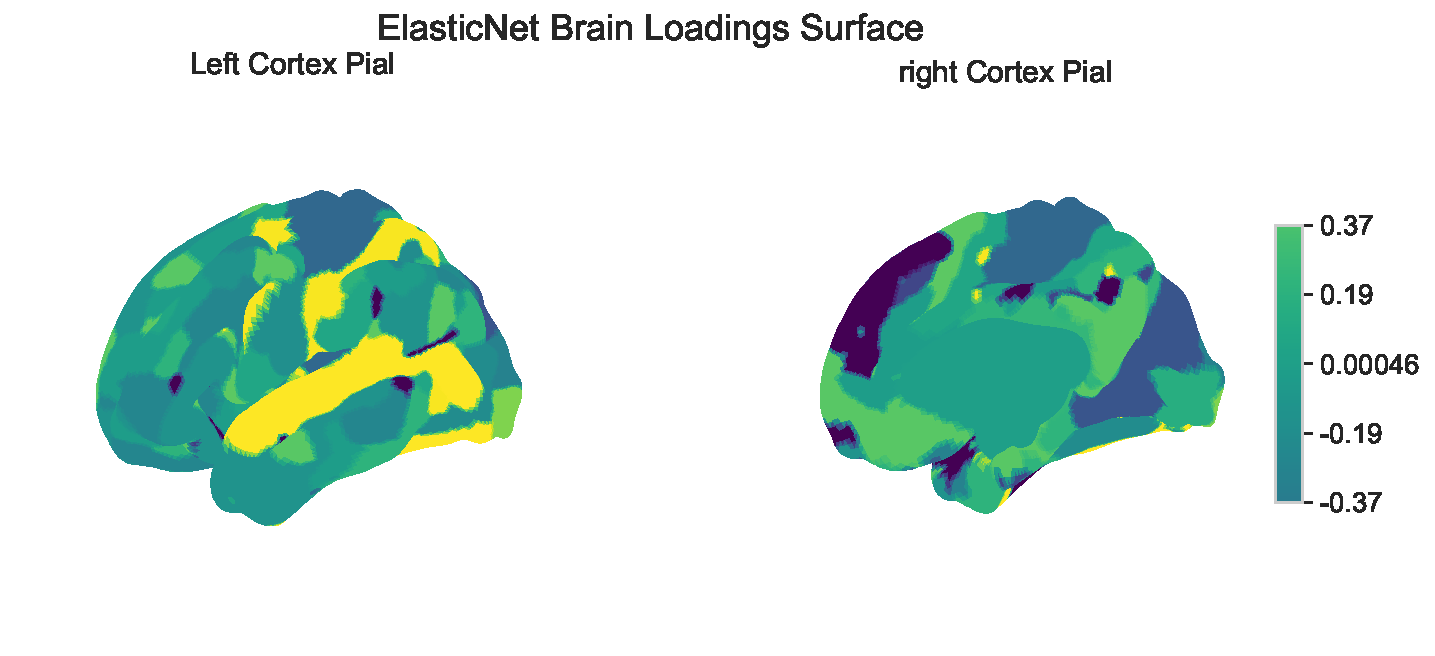
\includegraphics[width=0.49\linewidth]{figures/regularization/hcp/ElasticNet brain loadings}
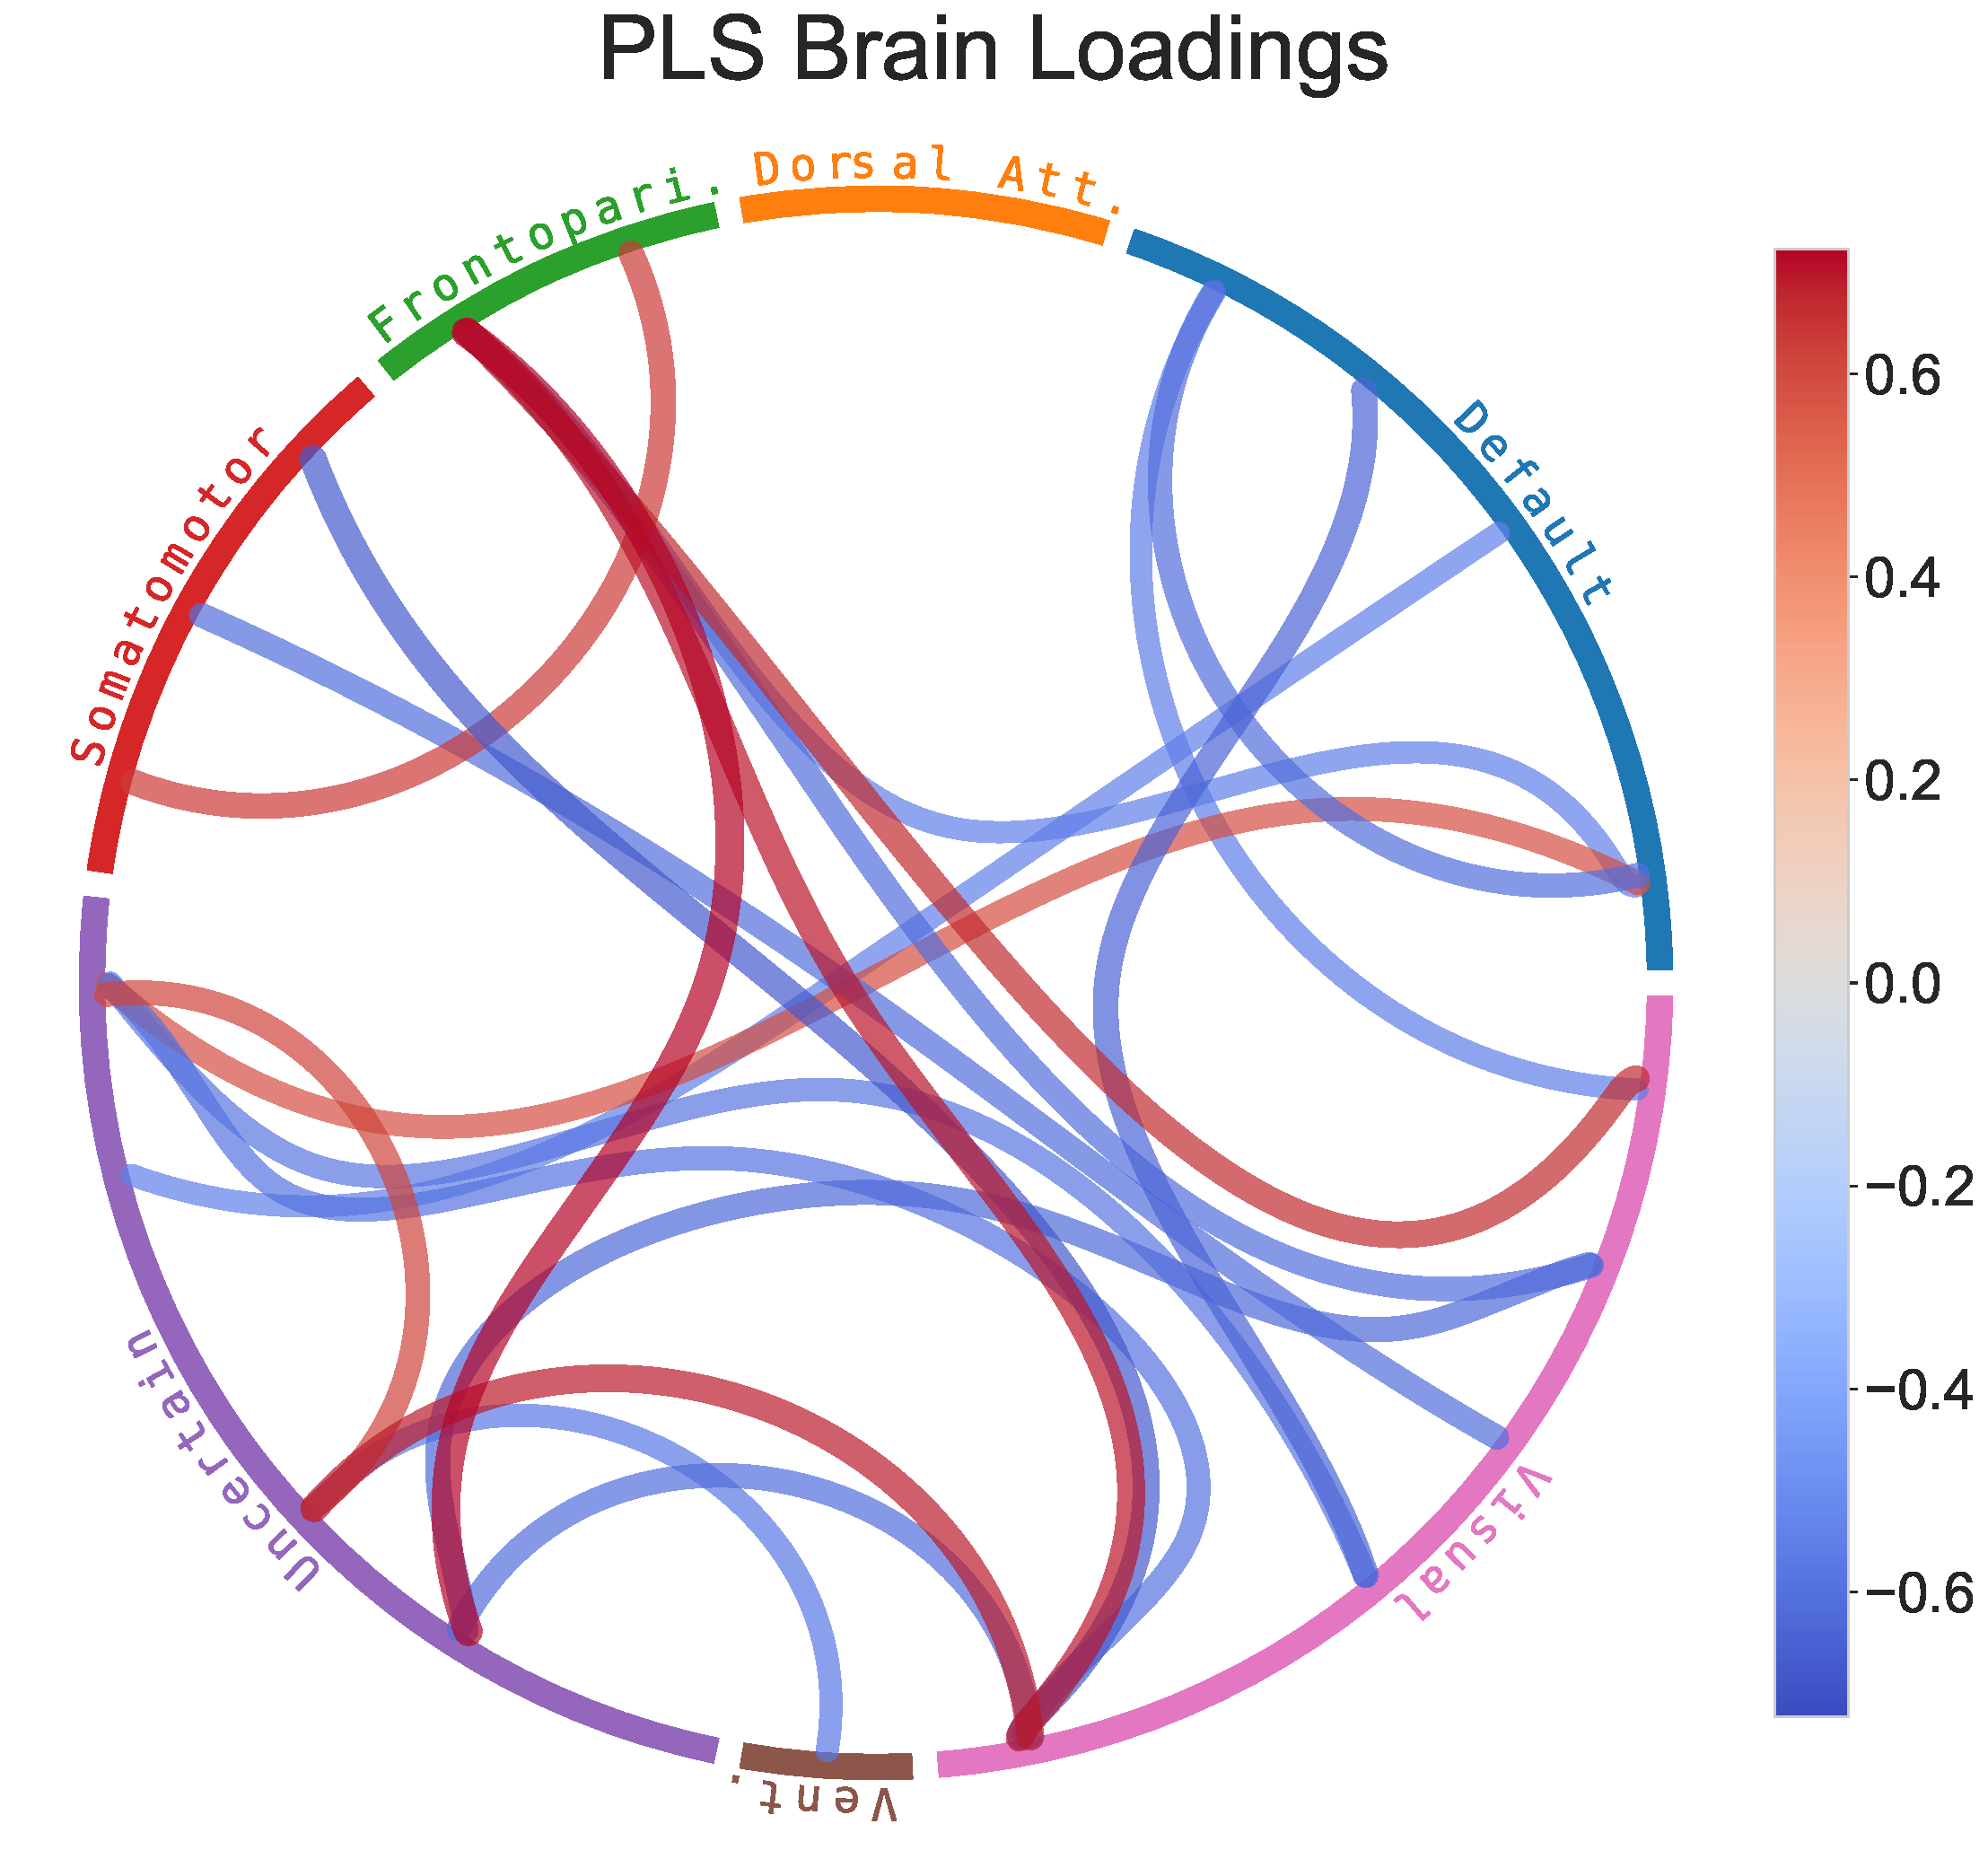
\includegraphics[width=0.49\linewidth]{figures/regularization/hcp/PLS brain loadings}
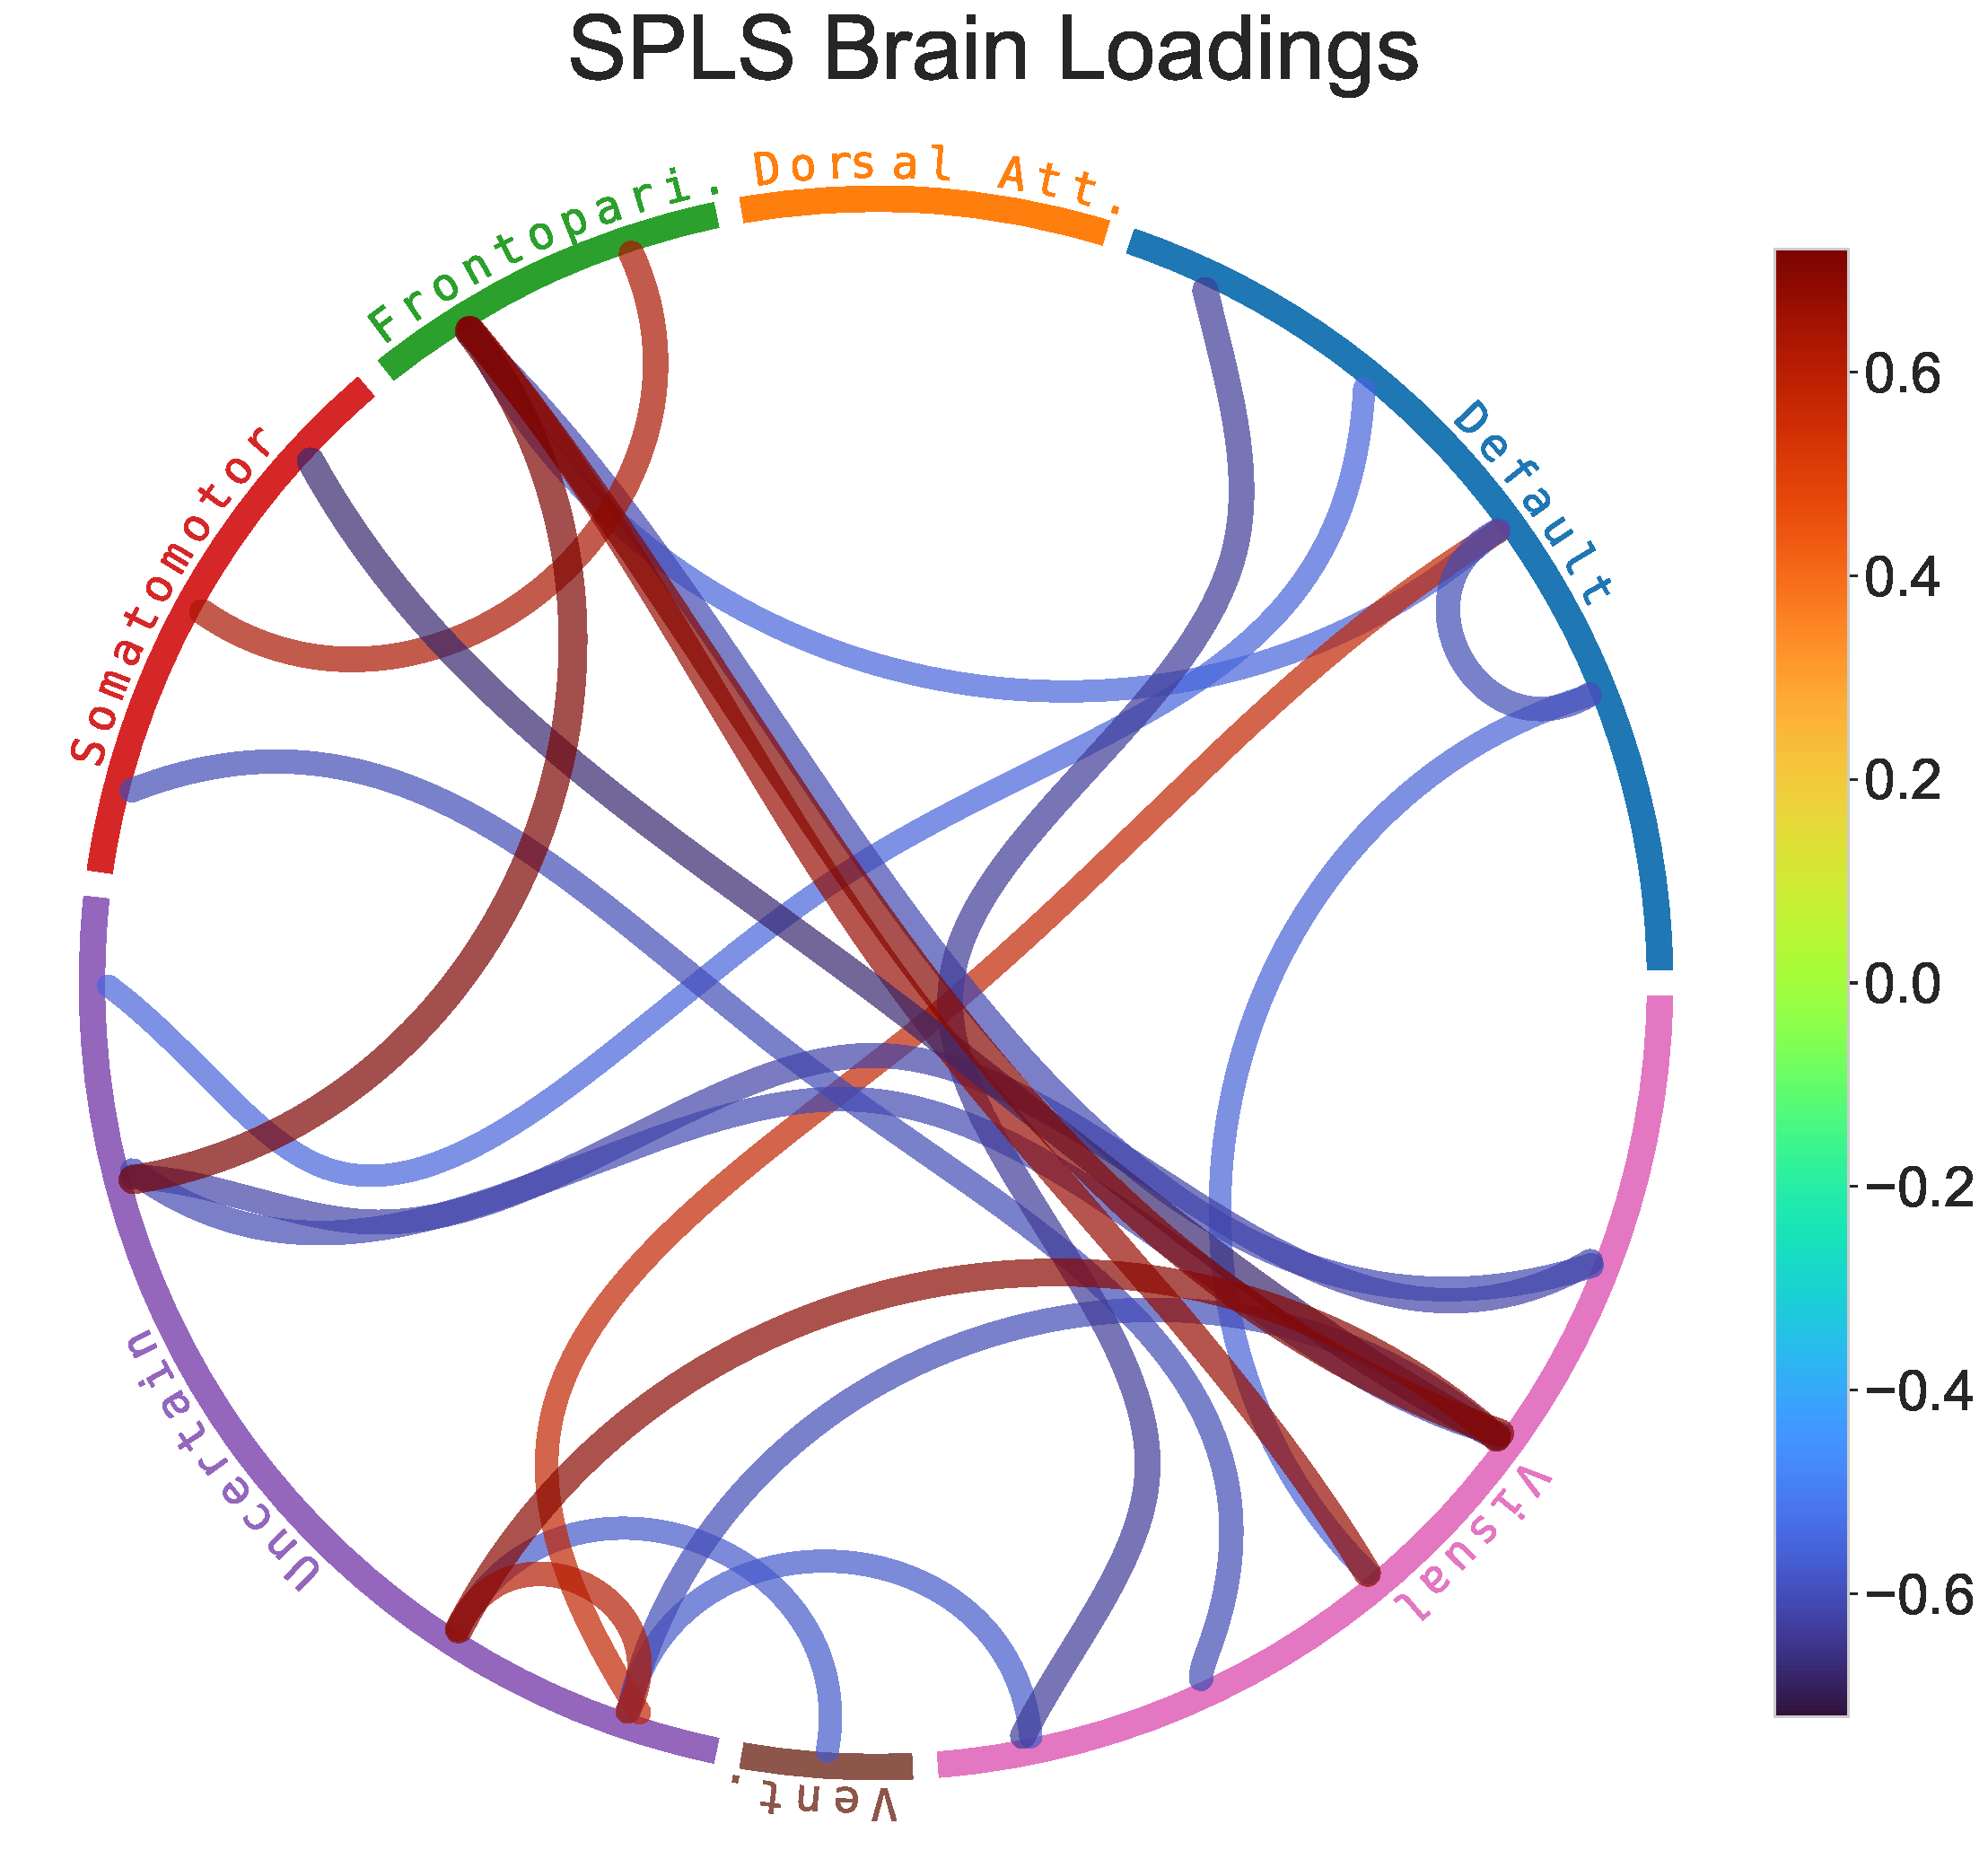
\includegraphics[width=0.49\linewidth]{figures/regularization/hcp/SPLS brain loadings}
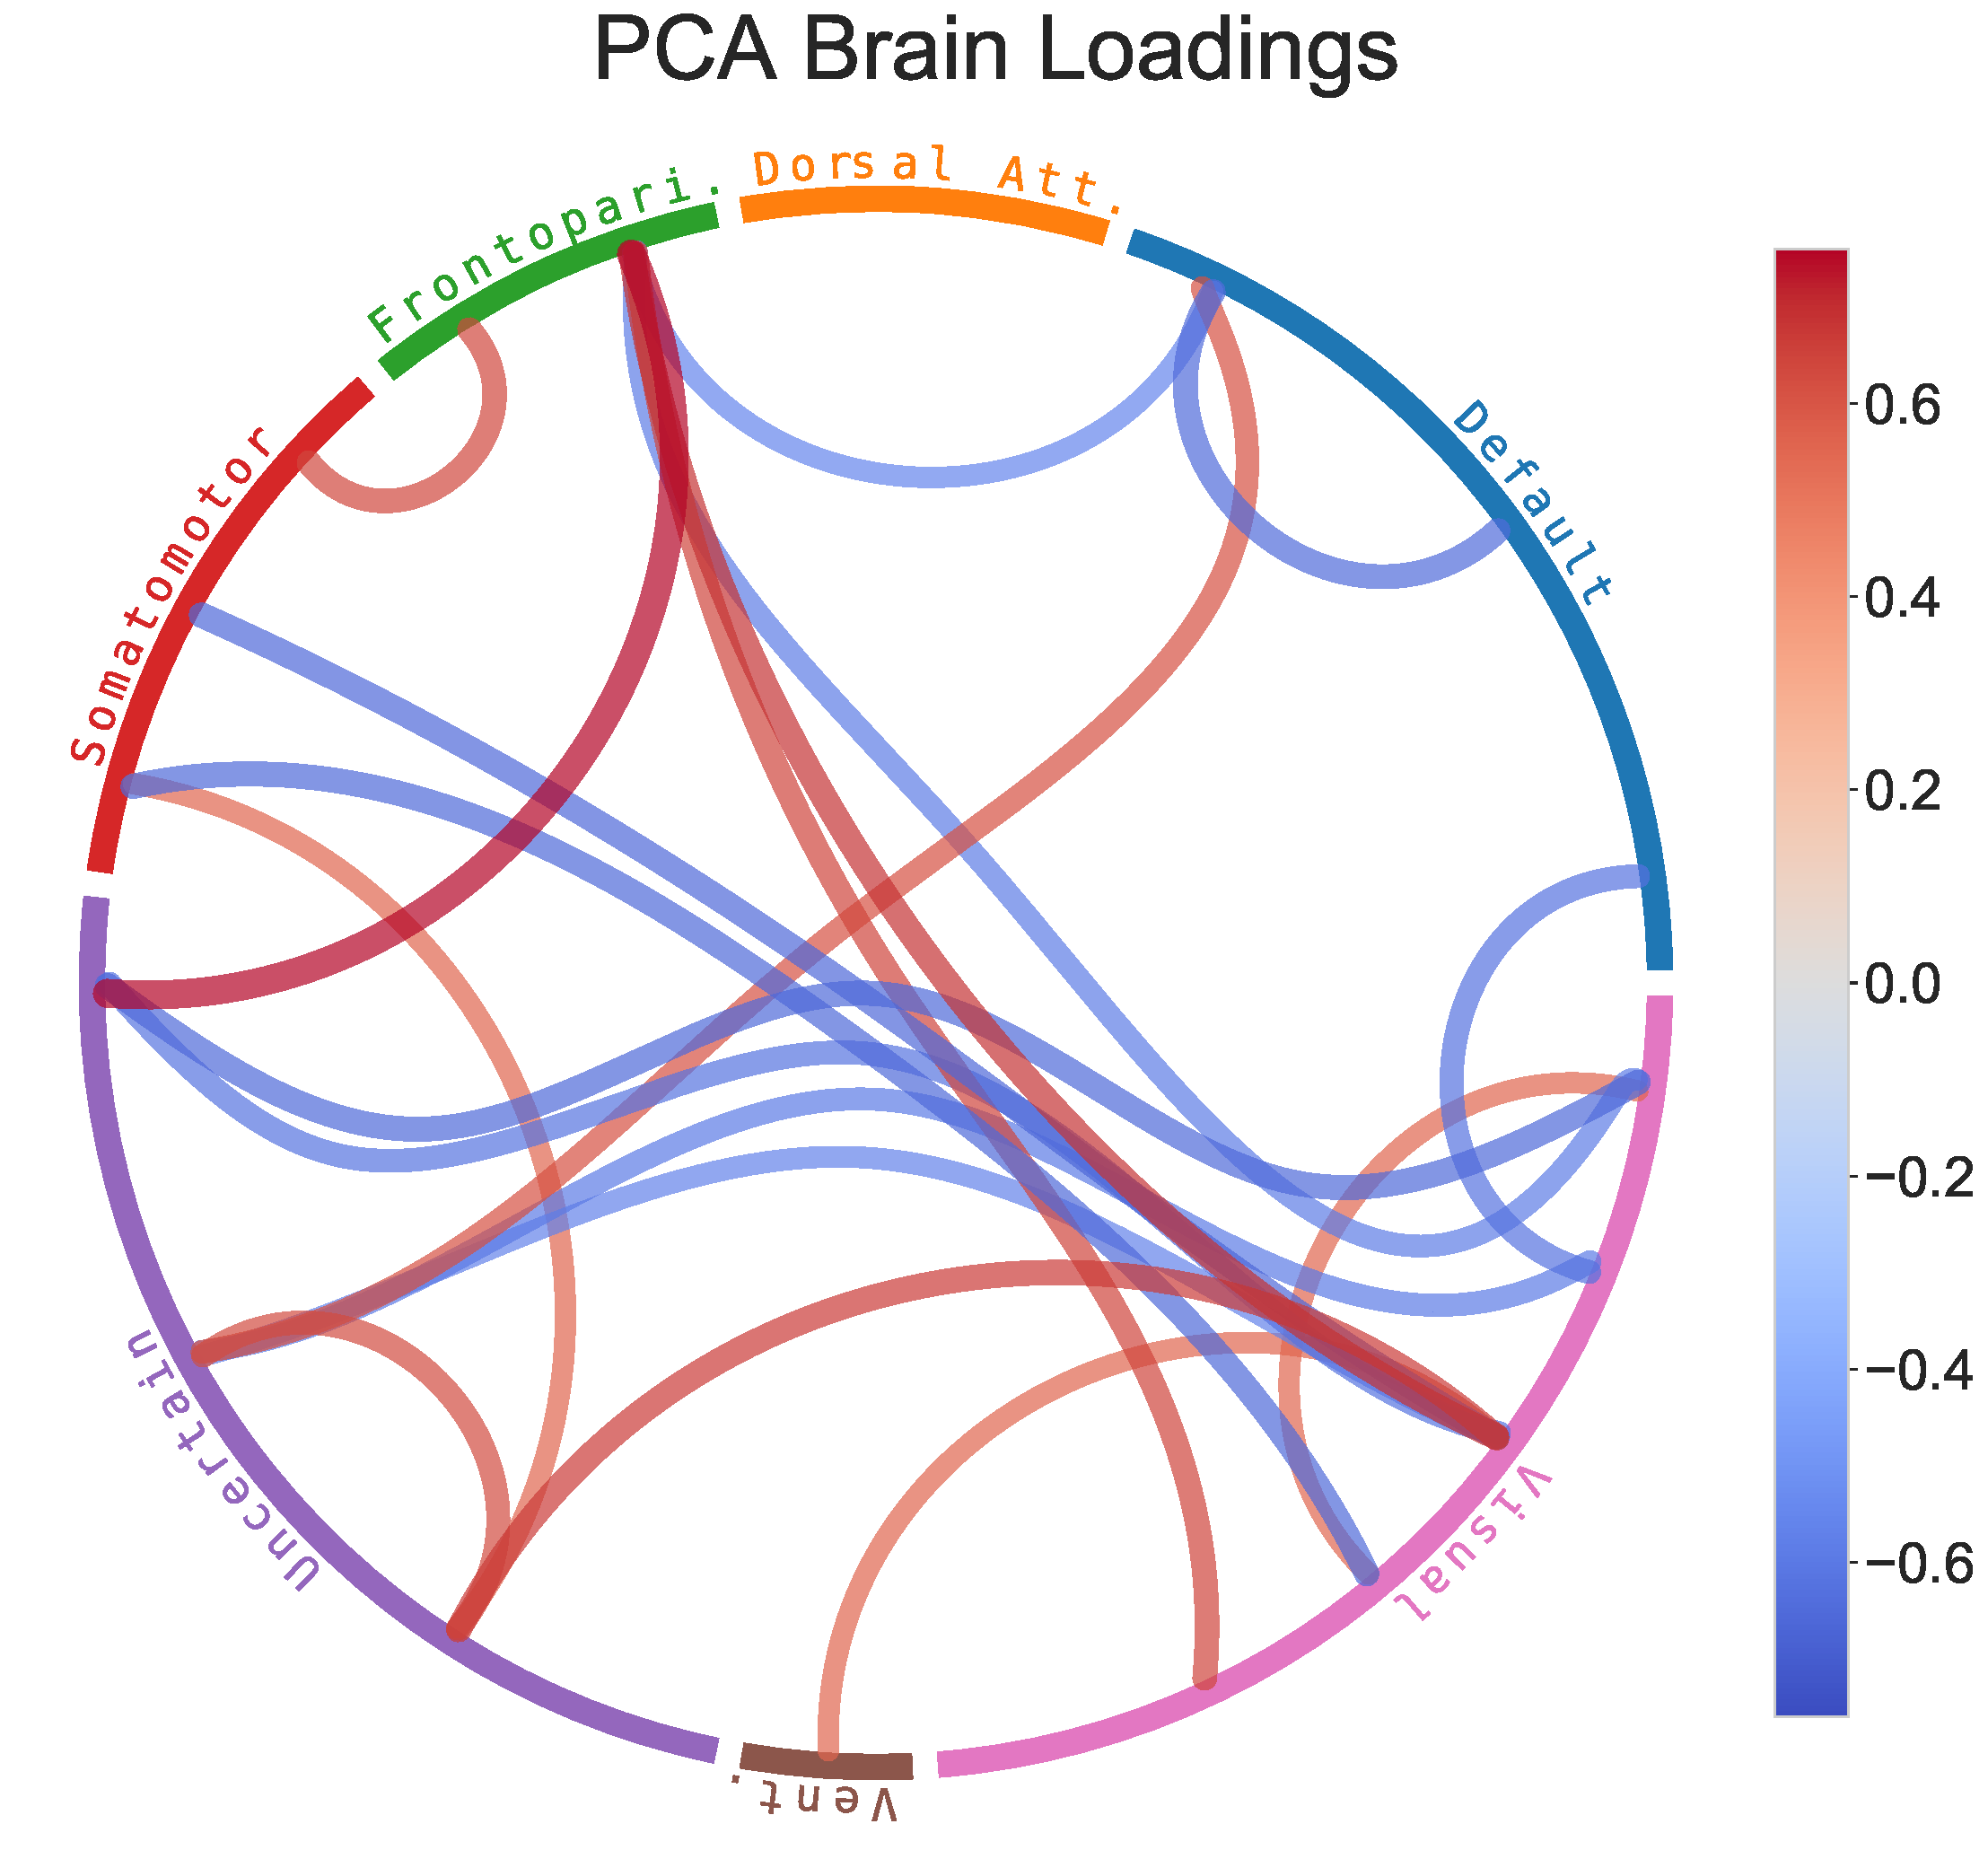
\includegraphics[width=0.49\linewidth]{figures/regularization/hcp/PCA brain loadings}
\caption{Chord diagrams of the top 8 positive and negative brain loadings for each model.}\label{fig:chord_loadings}
\end{figure}

\paragraph{Surface Map Parcellations}
The brain surface plots in Figure~\ref{fig:brain} represent maps of brain connection strength increases/decreases, which
were obtained by weighting each node’s parcel map with the GFA edge-strengths summed across the edges
connected to the node.
In Figure~\ref{fig:brain}, we show increases on the left and decreases on the right.

\textcolor{red} Need to find something biologically useful to say about these.
%
%\begin{figure}
%\centering
%\includegraphics[width=\linewidth]{figures/regularization/hcp/PCA brain loadings surface}
%\includegraphics[width=\linewidth]{figures/regularization/hcp/RCCA brain loadings surface}
%\includegraphics[width=\linewidth]{figures/regularization/hcp/ElasticNet brain loadings surface}
%\includegraphics[width=\linewidth]{figures/regularization/hcp/PLS brain loadings surface}
%\includegraphics[width=\linewidth]{figures/regularization/hcp/SPLS brain loadings surface}
%\caption{Map of CCA connection strength variations, with each node’s parcel map weighted by CCA edge-strength changes across edges involving that node.}\label{fig:brain}
%\end{figure}

\subsubsection{Sparsity of Weights}

Table \ref{tab:brain-behaviour-weights-hcp} shows the number of non-zero weights for each model.
We can see that tuned SPLS and Elastic Net do find sparse weights, but given the minimal difference in performance, it is not convincing evidence that this is a useful property.

\begin{table}[h]
\centering
\caption{Number of non-zero weights for each model.}
\begin{tabular}{|c|c|c|}
\hline
Model &  Brain Weights &  Behaviour Weights \\
\hline
PCA        &            300 &                145 \\
RCCA       &            300 &                145 \\
Elastic Net &            241 &                 96 \\
PLS        &            300 &                145 \\
SPLS       &            118 &                 56 \\
\hline
\end{tabular}\label{tab:brain-behaviour-weights-hcp}
\end{table}

\newpage
\subsection{Alzheimer's Disease Neuroimaging Initiative (ADNI) Data}\label{subsec:adni}

We now turn to the ADNI data where our analysis is similar but visualized differently.
This is because the ADNI data contains structural MRI data rather than functional MRI data.

\subsubsection{Out of Sample Correlation}

In this experiment, the Elastic Net model outperformed all other models in terms of out-of-sample correlation (Figure~\ref{fig:performance}).
The RCCA model also outperformed the PLS and SPLS models while SPLS outperformed PLS.
Suprisingly, PCA performed almost as well as PLS.

\begin{figure}
\centering
\includegraphics[width=0.5\linewidth]{figures/regularization/adni/holdout_correlations}
\caption{Out-of-sample canonical correlations for each model.}\label{fig:performance}
\end{figure}

\subsubsection{Behaviour Weights and Loadings}

As for the HCP data, Figure \ref{fig:adni-beh} plot the top 8 positive and negative non-imaging loadings and their associated weights for each model.
Some of the identified behavioural loadings including a number of orientation tests are similar across all of the models including even PCA.
This is indicative of the strong shared signal between the behavioural data and the brain structure data.
SPLS and Elastic Net both hone in on the orientation and recall tests in the weight space which appears also to translate to the loadings space.
The RCCA and Elastic Net models are suprisingly different in both the weight and loadings space, with the RCCA loading on a couple of attention and calculation tests in addition to the ubiquitous orientation and recall tests.

\begin{figure}
\centering
\includegraphics[width=0.8\linewidth]{figures/regularization/adni/PCA behaviour weights and loadings}
\includegraphics[width=0.8\linewidth]{figures/regularization/adni/RCCA behaviour weights and loadings}
\includegraphics[width=0.8\linewidth]{figures/regularization/adni/ElasticNet behaviour weights and loadings}
\includegraphics[width=0.8\linewidth]{figures/regularization/adni/PLS behaviour weights and loadings}
\includegraphics[width=0.8\linewidth]{figures/regularization/adni/SPLS behaviour weights and loadings}
\caption{Bar plots of the behaviour weights and loadings for each model.}\label{fig:adni-beh}
\end{figure}

\subsubsection{Brain Structure Weights and Loadings}

We plot the weights and loadings as a mosaic plot with 3 slices in each direction in Figure~\ref{fig:adni-brain}.
Previous work using SPLS with the ADNI dataset identified the same striking pattern of weights with the model strikingly selecting the hippocampal weights\cite{monteiro2016multiple}.
While the Elastic Net has a less visually appealing selection of weights, with a honeycomb pattern near the edges of the brain, the hippocampal region is more clearly loaded on in the loadings space (and likewise for RCCA).
It is noticeable that PCA, PLS and SPLS both weights in the same direction whereas RCCA and Elastic Net weight different regions with opposite signs.

\begin{figure}
\centering
\includegraphics[width=0.45\linewidth]{figures/regularization/adni/PCA brain loadings mosaic}
\includegraphics[width=0.45\linewidth]{figures/regularization/adni/PCA brain weights mosaic}
\includegraphics[width=0.45\linewidth]{figures/regularization/adni/RCCA brain loadings mosaic}
\includegraphics[width=0.45\linewidth]{figures/regularization/adni/RCCA brain weights mosaic}
\includegraphics[width=0.45\linewidth]{figures/regularization/adni/ElasticNet brain loadings mosaic}
\includegraphics[width=0.45\linewidth]{figures/regularization/adni/ElasticNet brain weights mosaic}
\includegraphics[width=0.45\linewidth]{figures/regularization/adni/PLS brain loadings mosaic}
\includegraphics[width=0.45\linewidth]{figures/regularization/adni/PLS brain weights mosaic}
\includegraphics[width=0.45\linewidth]{figures/regularization/adni/SPLS brain loadings mosaic}
\includegraphics[width=0.45\linewidth]{figures/regularization/adni/SPLS brain weights mosaic}
\caption{Statistical maps of brain structure loadings and weights for each model.}\label{fig:adni-brain}
\end{figure}

\subsubsection{Sparsity of Weights}

Table~\ref{tab:brain-behaviour-weights-adni} once again shows the number of non-zero weights for each model.
We can see that tuned SPLS and Elastic Net once again identify sparse weights.
In this case, the difference in performance is more convincing and suggests that this sparsity is less spuriously induced than for the HCP data.
This is supported by the fact that Elastic Net and SPLS models find a similar level of sparsity in the brain weights.
On the other hand SPLS finds a much sparser set of behavioural weights.

\begin{table}[h]
\centering
\caption{Number of non-zero weights for each model.}
\begin{tabular}{|c|c|c|}
\hline
Model &  Brain Weights &  Behaviour Weights \\
\hline
PCA        &         168130 &                 31 \\
RCCA       &         168130 &                 31 \\
Elastic Net &          59617 &                 17 \\
PLS        &         168130 &                 31 \\
SPLS       &          74995 &                 10 \\
\hline
\end{tabular}\label{tab:brain-behaviour-weights-adni}
\end{table}

\subsubsection{Identitiness of Covariance Matrices}
In this section, we consider the identitiness of the covariance matrices for the HCP and ADNI datasets.
Figure \ref{fig:covariance-eigenvalues-real} shows the eigenvalues of the covariance matrices for the HCP and ADNI datasets while Figure \ref{fig:covariance-matrices-real} shows the covariance matrices themselves (with the ADNI brain covariance matrix left out due to its size).
From Figure \ref{fig:covariance-eigenvalues-real}, we can see that the eigenvalues of the covariance matrices for the ADNI data are much closer to the ideal for identity covariance than for the HCP data.
\begin{figure}
\centering
\includegraphics[width=0.8\linewidth]{figures/regularization/covariance/hcp_adni_covariance_eigenvalues}
\caption{Eigenvalues of the covariance matrices for the HCP and ADNI datasets.}\label{fig:covariance-eigenvalues-real}
\end{figure}

From Figure \ref{fig:covariance-matrices-real}, we can see the block structure of the covariance matrices.

\begin{figure}
\centering
\begin{subfigure}{0.66\linewidth}
\centering
\includegraphics[width=\linewidth]{figures/regularization/covariance/HCP_covariance}
\caption{HCP}
\end{subfigure}
%
\begin{subfigure}{0.33\linewidth}
\centering
\includegraphics[width=\linewidth]{figures/regularization/covariance/ADNI_covariance}
\caption{ADNI}
\end{subfigure}
\caption{Covariance matrices for the HCP and ADNI datasets.}
\label{fig:covariance-matrices-real}
\end{figure}

This suggests that the only dataset and view where we can expect sparsity on the weights to imply sparsity on the loadings is the ADNI data and is consistent with the results we have seen in the previous section, that sparsity improves performance in the ADNI data but not in the HCP data.

\section{Discussion and Limitations}

In this section, we discuss the implications of our findings as well as the limitations of our study and the proposed FRALS method, some of which we address in later chapters of this thesis.

\subsection{Discussion}

\paragraph{Interpreting the Forward and Backward Models of CCA:} Consistent with \cite{haufe2014interpretation}, we have shown that assumptions imposed on the weights of a model do not in general transfer to the loadings.
This is because the weights and loadings are only equivalent when the covariance matrices are identity.
We have gone a step further than \cite{haufe2014interpretation} by showing that the identitiness of the covariance matrices is crucial for understanding how imposing sparsity on the weights imposes a prior belief in sparsity on the more biologically interesting loadings.

\paragraph{Sparsity on the weights does not imply sparsity on the loadings:}

On the other hand, our results raise the question of whether sparsity on the weights makes sense in the first place.
For latent variable models of brain-behaviour associations, we have argued that the loadings are the more biologically relevant quantity.
Since in practice, identity covariance is rarely a good assumption, the weights and loadings are not equivalent.
This means that sparsity on the weights does not imply sparsity on the loadings, and so we should not expect sparsity on the weights to lead to more interpretable loadings.
A practical step this implies is \textit{to ensure that the data covariances are at least close to identity before applying sparse CCA methods}.

\paragraph{Identitiness of real covariance matrices:} Between the HCP and ADNI datasets, only the ADNI data had eigenvalue spectra that were reasonably close to those of an identity matrix.
This suggests that the only dataset and view where we can expect sparsity on the weights to imply sparsity on the loadings is the ADNI data and is consistent with the results we have seen in the previous section, that sparsity improves performance in the ADNI data but not in the HCP data.
Furthermore, the loadings and weights are much more similar to each other in the ADNI data than in the HCP data, supporting the idea that the ADNI weights are themselves somewhat interpretable as estimates of the biologically relevant loadings.
Finally, in the well understood Alzheimer's disease data, we know that the identified weights (and loadings) are consistent with the known biology of the disease.

\paragraph{Sample versus Population Setting:} The results from the simulated data illustrate the disparities that can arise between population and sample settings.
Although PLS, RCCA, and CCA are equivalent under isotropic noise in a population framework, experiments showed that their performance can vary substantially in a sample setting.
In particular, this manifested as PLS underperforming RCCA and CCA under isotropic noise \textit{even though this is exactly the scenario where covariance identity holds and covariance thus equals correlation}.
This is because the sample covariance matrix is not the same as the population covariance matrix and PLS is sensitive to even small differences in the principal components of the sample covariance matrix.
Furthermore, in limited sample sizes, our estimations of the covariance matrices are not accurate, and so the identitiness of the covariance matrices is not guaranteed.
This generally resulted in poor estimation of loadings from model weights \textit{even when the weights themselves were estimated almost perfectly}.
Therefore, it's crucial for researchers to recognize these nuances and adopt appropriate measures when extrapolating results, especially in brain-behavior studies where typically only one sample is available and often limited in size.

\paragraph{Ridge CCA is typically much better than PLS across datasets:} Our results show that Ridge CCA is typically much better than PLS across datasets.
Much like regularised regression, it is unusual to need to use maximal ridge regularization even in high dimensions.
Our results in simulated data even cast doubt on the touted stability of PLS over CCA with respect to population CCA problem.
This means that while PLS might be more stable for a given dataset, it is not necessarily more stable across random samples from the same population.

\paragraph{Can We Construct a Regularization Functional that Imposes Sparsity on the Loadings?}
Finally, given our observations, a natural question to ask is whether we can construct a regularization functional that imposes sparsity on the loadings (instead of the weights).
The answer is yes, but it is not straightforward and in the small sample setting, it is not clear that it is a good idea.
The principle would be much the same as the Lasso, but we would need to use the sample covariance matrix to define the norm:

\begin{align}
    P(W)=\|W\|_1 \\
    P(L)=\|\hat{\Sigma}U\|_1
\end{align}

Which imposes an L1 penalty on the loadings via an L1 penalty on the weights multiplied by the sample covariance matrix.
We could in principle apply the soft-thresholding operator to the estimated loadings.
However we would need to be careful to ensure that the sample covariance matrix is invertible in order to get back to the weights.
This is of course not guaranteed in the small sample setting.

\subsection{Experiment Limitations}

\paragraph{Non-Gaussian Data:} The simulated data was generated from a Gaussian distribution.
This is a limitation of our study, and it would be interesting to see how the models perform on non-Gaussian data.
In particular, biomedical data typically contain categorical and even binary variables, and so it would be interesting to see how the models perform on such data.
We show an example of the Orientation category scores in the ADNI data in Figure~\ref{fig:adni-behavioural-data}.

\begin{figure}
\centering
\includegraphics[width=\linewidth]{figures/regularization/adni/Orientation}
\caption{Histogram of the Orientation test scores in the ADNI data.}\label{fig:adni-behavioural-data}
\end{figure}

\section{Conclusion}\label{sec:conclusion}

In this chapter, we have explored the performance of several CCA variants on simulated and real data.
We have shown that the choice of CCA variant can have a significant impact on the results.
We have also shown that the identitiness of the covariance matrices is crucial for understanding how imposing sparsity on the weights imposes a prior belief in sparsity on the more biologically interesting loadings.
We described a way to check the identitiness of the covariance matrices by looking at the eigenvalues of the covariance matrices and comparing to the ideal case.
We have also shown that FRALS can be a useful tool for brain-behaviour studies, but that it is computationally expensive.

In the next chapter, we address the scalability of CCA and its variants by introducing a novel algorithm based on gradient descent.
\graphicspath{{chapters/gradient_descent/}}


\chapter{Efficient Algorithms for the CCA Family: Unconstrained Losses with Unbiased Gradients}\label{chap:gradient_descent}
\epigraph{It seems easier to train a bi-directional LSTM with attention than to compute the SVD of a large matrix}{Chris Ré}\cite{gemp2021}
\minitoc
% chktex-file 44
% chktex-file 3
\section*{Preface}
The content of this chapter is based on a series of papers~\citep{chapman2022generalized, chapman2023efficient} as well as a NeurIPS workshop paper~\citep{chapman2023neurips}.
I am grateful to my co-authors Lennie Wells and Ana Lawry Aguila for their contributions to this work.
In particular, Lennie's mathematical expertise improved the theoretical grounding of the idea greatly and Ana's access to the UK Biobank dataset enabled the application of our methods to a real-world biomedical dataset.
In this thesis I include much of the work from these papers, but I exclude many of Lennie's extensive proofs where I can make no claim to have contributed beyond proofreading.

\section{Introduction}

There are significant computational challenges when applying these CCA methods to large scale data.



Classical algorithms for linear CCA methods require computing full covariance matrices and so scale quadratically with dimension, becoming intractable for many large-scale datasets of practical interest.
There is therefore great interest in approximating solutions for CCA in stochastic or data-streaming settings \citep{arora2012stochastic}.




\section{Background: Efficient CCA}\label{sec:background-unified}

\subsubsection{Challenges in Solving Generalized Eigenvalue Problems}

The GEP is often represented as \( Ax = \lambda Bx \), where \( A \) and \( B \) are matrices. To generalize the dimensions of these matrices, let's denote them as \( m \times m \). This dimension \( m \) can vary based on the specific method in use. For instance, in Principal Component Analysis (PCA), represented as \acrshort{pca}, \( m \) would be equal to \( p \) since \( A \) and \( B \) are \( p \times p \) matrices. In methods like Partial Least Squares (PLS) and Canonical Correlation Analysis (CCA), represented as \acrshort{pls} and \acrshort{cca} respectively, \( m \) would be \( p_1+p_2 \), as \( A \) and \( B \) in these cases are \( (p_1+p_2) \times (p_1+p_2) \).


% Table summarizing the definitions of A and B for various methods
\begin{table}[h]
    \centering
    \begin{tabular}{|c|c|c|c|c|}
        \hline
        Method         & \( A \)           & \( B \)   & \( x \)        & Dimensions       \\
        \hline
        \acrshort{pca} & \( \Sigma_{11} \) & \( I \)   & \( u\sps{1} \) & \( p \times p \) \\
        \hline
        LDA            & \( S_B \)         & \( S_W \) & \( u\sps{1} \) & \( p \times p \) \\
        \hline
        \acrshort{cca} & \( \begin{pmatrix}
                                \Sigma_{11} & \Sigma_{12} \\ \Sigma_{21} & \Sigma_{22}
        \end{pmatrix} \) & \( \begin{pmatrix}
                                  \Sigma_{11} & 0 \\ 0 & \Sigma_{22}
        \end{pmatrix} \) & \( \begin{pmatrix}
                                  u\sps{1} \\ u\sps{2}
        \end{pmatrix} \) & \( (p_1+p_2) \times (p_1+p_2) \) \\
        \hline
        \acrshort{pls} & \( \begin{pmatrix}
                                0 & \Sigma_{12} \\ \Sigma_{21} & 0
        \end{pmatrix} \) & \( I \) & \( \begin{pmatrix}
                                            u\sps{1} \\ u\sps{2}
        \end{pmatrix} \) & \( (p_1+p_2) \times (p_1+p_2) \) \\
        \hline
    \end{tabular}
    \caption{Definitions and dimensions of \( A \)and \( B \)for different subspace learning methods.}
    \label{tab:subspace}
\end{table}

To solve the GEP, one common technique is to transform it into a standard eigenvalue problem \( B^{-\frac{1}{2}} A B^{-\frac{1}{2}} y = \lambda y \), followed by eigendecomposition.
However, this approach has computational complexity \( O((p_1+p_2)^3) \) and may suffer from numerical instability.

\subsubsection{\acrshort{pca}-CCA}

One way to reduce the complexity of solving GEPs is to use the \acrshort{pca}-CCA method, which first applies \acrshort{pca} to the data and then solves the GEP in the reduced space.
An important advantage of using \acrshort{pca}-CCA is computational efficiency, especially for high-dimensional data.
The overall complexity of \acrshort{pca}-CCA involves two main steps.
First, applying PCA has a complexity of \( O(p_1^3+ p_2^3) \), dominated by the larger of the two matrices.
Second, solving the generalized eigenvalue problem in the reduced space with \( K \) components in each view leads to a complexity of \( O((2K)^3) \).
Thus, the overall complexity of \acrshort{pca}-CCA is \( O(p_1^3+ p_2^3) + (2K)^3) \), which is significantly lower than the complexity of solving the GEP directly.
Since CCA, ridge CCA, and PLS can all be solved in the principal component space, \acrshort{pca}-CCA can be used to compute solutions efficiently \textit{even if we keep all the principal components}.
Most obviously, this is the case when the number of samples \( n \) is smaller than either of the number of features \( p_1 \) or \( p_2 \), i.e. \( n < p_1 \) or \( n < p_2 \).
In this case the maximum number of principal components is \( K=n \), and the complexity of PCA is \( O(n^3+ n^3) \) so that the overall complexity of \acrshort{pca}-CCA is thus \( O(2n^3+(2n^3)^3) \) = \( O(10n^3) \).
For fat data where \( p_1 \) and \( p_2 \) are larger than \( n \), we can reasonably expect $10n^3<p_1^3+ p_2^3$ and thus \acrshort{pca}-CCA is still more efficient than solving the original GEP.
This approach has been employed to great effect in neuroimaging but suprisingly is not used even in the scikit-learn implementation of \acrshort{cca} \citep{pedregosa2011scikit}.
Nonetheless, for the large sample sizes (desirable for machine learning frameworks as well as statistical power), the complexity of even \acrshort{pca}-CCA can render the problems nearly intractable.

\subsubsection{Kernel CCA}

Kernel \acrshort{cca} (\acrshort{kcca}) also offers computational efficiency for high-dimensional data (\(p_i>n\)) as its complexity scales with the number of samples \(n\), not the number of features \(p_i\).
It casts the CCA optimisation as a dual problem:

\begin{align}
    & \alpha_{\text{opt}}=\underset{\alpha_{\text{opt}}}{\mathrm{argmax}}\{ \alpha\sps{1}K\spsT{1}K\sps{2}\alpha\sps{2}  \} \\
    & \text{subject to:} \notag                                                                                            \\
    & \alpha\sps{1}K\spsT{1}K\sps{1}\alpha\sps{1}=1 \notag                                                                  \\
    & \alpha\sps{2}K\spsT{2}K\sps{2}\alpha\sps{2}=1 \notag
\end{align}

Where \(\alpha\sps{1}=\)

The kernel function in KCCA can be computed iteratively on pairwise comparisons of samples, allowing for memory efficiency by not requiring the entire dataset to be loaded into RAM.
This iterative approach uses slow hard drive memory access instead of RAM, making KCCA RAM memory-efficient but slower.
However, a significant drawback of KCCA is the need for access to all training data at test time, which raises concerns about efficiency and scalability.

\subsection{Stochastic PLS and CCA}
Recently, a number of algorithms have been proposed to approximate GEPs including PCA and PLS \citep{arora2012stochastic}, and CCA specifically \citep{bhatia2018gen}, in the `stochastic' or `data-streaming' setting; these can have big computational savings.
Typically, the computational complexity of classical GEP algorithms is $\mathcal{O}\left((n + k)p^2\right)$; by exploiting parallelism (both between eigenvectors and between samples in a mini-batch), we can reduce this down to $\mathcal{O}\left(d k \right)$ \citep{arora2016stochastic}.
Stochastic algorithms also introduce a form of regularisation which can be very helpful in these high-dimensional settings.
To the best of our knowledge, the state-of-the-art in Stochastic PLS and CCA are the subspace Generalized Hebbian Algorithm (SGHA) \citep{chen2019constrained} and $\gamma$-EigenGame \citep{gemp20,gemp2021}.
Specifically, SGHA utilizes a Lagrange multiplier heuristic along with saddle-point analysis, albeit with limited convergence guarantees.
EigenGame focuses on top-k subspace learning but introduces an adaptive whitening matrix in the stochastic setting with an additional hyperparameter.

\section{Methods: Novel Objectives and Algorithms}\label{sec:contributions}

In this section, we introduce a novel class of objectives for GEPs, which we call the Eckhart--Young (EY) objectives. They can be applied to any GEP, including CCA, PLS, and PCA but we will focus on CCA.

\subsection{Unconstrained objective for GEPs}\label{sec:gep-ey-formulation}
First, we present proposition \ref{prop:EY-charac}, a formulation of the top-$K$ subspace of GEP problems, which follows by applying the Eckhart--Young--Minsky inequality \citep{stewart_matrix_1990} to the eigen-decomposition of $B^\mhalf A B^\mhalf$. However, making this rigorous requires some technical care which we defer to the proof in supplement \ref{supp:proofs}.

\begin{restatable}[Eckhart--Young inspired objective for GEPs]{proposition}{EYcharac}
    \label{prop:EY-charac}
    The top-$K$ subspace of the GEP $(A,B)$ can be characterized by minimizing the following objective over $U \in \R^{D \times K}$:
    \begin{align}\label{eq:EY-charac}
    \LEYGEP(U) \defeq \tr \left( - 2\,U^T A U + \left(U^T B U\right) \left(U^T B U\right) \right)
    \end{align}
    Moreover, the minimum value is precisely $- \sum_{k=1}^K \lambda_k^2$, where $(\lambda_k)$ are the generalized eigenvalues.
\end{restatable}

This objective also has appealing geometrical properties.
It is closely related to a wide class of unconstrained objectives for PCA and matrix completion which have no spurious local optima \citep{ge_no_2017}, i.e. all local optima are in fact global optima.
This implies that certain local search algorithms, such as stochastic gradient descent, should indeed converge to a global optimum.

\begin{restatable}{proposition}{NoSpuriousLocalMinima}[No spurious local minima]\label{prop:no-spurious}
The objective $\LEYGEP$ has no spurious local minima.
That is, any matrix $\bar{U}$ that is a local minimum of $\LEYGEP$ must in fact be a global minimum.
\end{restatable}

It is also possible to make this argument quantitative by proving a version of the strict saddle property from \cite{ge_no_2017,ge2015escaping}; we state an informal version here and give full details in \cref{supp:tractable-optimization}.

\begin{corollary}[Informal: Polynomial-time Optimization]
    Under certain conditions on the eigenvalues and generalized eigenvalues of $(A,B)$, one can make quantitative the claim that:
    any $U_K \in \R^{D \times K}$ is either close to a global optimum, has a large gradient $\nabla \LEYGEP$, or has Hessian $\nabla^2 \LEYGEP$ with a large negative eigenvalue.

    Therefore, for appropriate step-size sequences, certain local search algorithms, such as sufficiently noisy SGD, will converge in polynomial time with high probability.
\end{corollary}

\subsection{Corresponding Objectives for the CCA family}
For the case of linear CCA we have $U^T A U = \sum_{i \neq j} \Cov(Z\sps{i}, Z\sps{j}), U^T B U = \sum_{i} \Var(Z\sps{i})$.
To help us extend this to the general case of nonlinear transformations, \cref{eq:general-form-of-representations}, we define the analogous matrices of total between-view covariance and total within-view variance
\begin{align}\label{eq:def-C-V-matrices}
\vphantom{\bigl(\bigr)} % increase vertical space
C(\theta) = \sum_{i \neq j} \Cov(Z\sps{i}, Z\sps{j}), \quad
V(\theta) = \sum_{i} \Var(Z\sps{i})
\end{align}
In the case of linear transformations, \cref{eq:cca-linear-function-def}, it makes sense to add a ridge penalty so we can define
\begin{align}\label{eq:v-alpha-ridge-definition}
V_\alpha(\theta) = \sum_i \alpha_i {U\spsT{i}} U\sps{i} +  (1 - \alpha_i) \Var(Z\sps{i})
\end{align}
This immediately leads to following unconstrained objective for the CCA-family of problems.
\begin{definition}[Family of EY Objectives]
    Learn representations $Z\sps{i} = f\sps{i}( X\sps{i}; \theta\sps{i})$ minimizing
    \begin{align}\label{eq:EY-loss-def-C-V}
    \LEY(\theta) = - 2 \tr C(\theta) + \norm{V_\alpha(\theta)}_F^2
    \end{align}
\end{definition}

\textbf{Unbiased estimates:}
since empirical covariance matrices are unbiased, we can construct unbiased estimates to $C, V$ from a batch of transformed variables $\Z$.
\begin{align}\label{eq:def-C-V-matrices-empirical}
\hat{C}(\theta)[\Z] = \sum_{i \neq j} \empCov(\Z\sps{i}, \Z\sps{j}), \quad
\hat{V}(\theta)[\Z] = \sum_{i} \empVar(\Z\sps{i})
\end{align}
In the linear case we can construct $\hat{V}_\alpha(\theta)[\Z]$ analogously by plugging sample covariances into \cref{eq:v-alpha-ridge-definition}.
Then if $\Z, \Z'$ are two independent batches of transformed variables, the batch loss
\begin{align}\label{eq:empirical-EY-loss-estimate-def}
\empLEY[\Z, \Z'] \defeq - 2 \tr \hat{C}[\Z] + \langle \hat{V}_\alpha[\Z], \hat{V}_\alpha[\Z'] \rangle_F
\end{align}
gives an unbiased estimate of $\LEY(\theta)$.
This loss is a differentiable function of $\Z, \Z'$ and so also of $\theta$.

\textbf{Simple algorithms:}
We first define a very general algorithm using these estimates in Algorithm \ref{alg:general}.
In the next section we apply this algorithm to multi-view stochastic CCA and PLS.

\begin{algorithm}
    \caption{GEP-EY: General algorithm for learning correlated representations}
    \label{alg:general}
    \begin{algorithmic}
        \STATE {\bfseries Input:} data stream of mini-batches $(\X(b))_{b=1}^\infty$ where each consists of $M$ samples from the original dataset. Learning rate $(\eta_t)_t$. Number of time steps $T$. Class of functions $f(\cdot; \theta)$ whose outputs are differentiable with respect to $\theta$.
        \STATE {\bfseries Initialize:} $\hat{\theta}$ with suitably random entries
        \FOR{$t=1$ {\bfseries to} $T$}
        \STATE Obtain two independent mini-batches \( \X(b), \X(b') \) by sampling \( b, b' \) independently
        \STATE Compute batches of transformed variables $\Z(b) = f(\X(b); \theta), \Z(b') = f(\X(b'); \theta)$
        \STATE Estimate loss $\empLEY(\theta)$ using \cref{eq:empirical-EY-loss-estimate-def}
        \STATE Obtain gradients by back-propagation and step with your favourite optimizer.
        \ENDFOR
    \end{algorithmic}
\end{algorithm}

\subsection{Applications to (multi-view) stochastic CCA and PLS}
\begin{lemma}[Objective recovers GEP formulation of linear (multi-view) CCA]
    When the $f\sps{i}$ are linear, as in \cref{eq:cca-linear-function-def}, the population loss from \cref{eq:EY-loss-def-C-V} recovers MCCA as defined in \cref{sec:CCA-family}.
\end{lemma}
\begin{proof}
    By construction, for linear MCCA we have $C = U^T A U,\, V_\alpha=U^T B_\alpha U$, where $(A, B_\alpha)$ define the GEP for MCCA introduced in \cref{eq:gep-most-general-formulation}.
    So $\LEY(U) = \LEYGEP(U)$ and by \cref{prop:EY-charac} the optimal set of weights define a top-$K$ subspace of the GEP, and so is a MCCA solution.
\end{proof}

Moreover, by following through the chain of back-propagation, we obtain gradient estimates in $\mathcal{O}(MKD)$ time.
Indeed, we can obtain gradients for the transformed variables in $\mathcal{O}(M K^2)$ time so the dominant cost is then updating $U$; we flesh this out with full details in \cref{supp:fast-updates}.

\section{Experiments}

\subsection{Stochastic CCA}
First, we compare our proposed method, CCA-EY, to the baselines of $\gamma$-EigenGame and SGHA.
Our experimental setup is almost identical to that of \cite{meng2021online, gemp2022generalized}; unlike \cite{gemp2022generalized} we do not simplify the problem by first performing PCA on the data before applying the CCA methods, which explains the decrease in performance of $\gamma$-EigenGame compared to their original work.
All models are trained for a single epoch with varying mini-batch sizes ranging from 5 to 100. We use Proportion of Correlation Captured (PCC) as our evaluation metric, defined as \( \text{PCC} = (\sum_{i=k}^K \rho_k)/ ({\sum_{k=1}^K \rho_k^*}) \) where $\rho_k$ are the full batch correlations of the learnt representations, and $\rho_k^*$ are the canonical correlations computed numerically from the full batch covariance matrices.

\textbf{Parameters:} For each method, we searched over a hyperparameter grid using \citet{wandb}.

\begin{table}[h!]
    \centering
    \begin{tabular}{|l|l|}
        \hline Parameter             & Values              \\
        \hline minibatch size        & 5,20,50,100         \\
        \hline components            & 5                   \\
        \hline epochs                & 1                   \\
        \hline seed                  & 1, 2, 3, 4, 5       \\
        \hline lr                    & 0.01, 0.001, 0.0001 \\
        \hline $\gamma$\footnotemark & 0.01,0.1,1,10       \\
        \hline
    \end{tabular}
    \footnotetext{gamma is only used for $\gamma$-EigenGame}
\end{table}

\textbf{Observations:}
Figure \ref{fig:scca_mediamill} compares the algorithms on the MediaMill dataset. \cref{fig:corr_mediamill} shows that CCA-EY consistently outperforms both $\gamma$-EigenGame and SGHA in terms of PCC across all evaluated mini-batch sizes.
\cref{fig:lr_mediamill} examines the learning curves for batch sizes 5 and 100 in more detail; CCA-EY appears to learn more slowly than SGHA at the start of the epoch, but clearly outperforms SGHA as the number of samples seen increases. $\gamma$-EigenGame significantly underperforms SGHA and CCA-EY, particularly for small batch sizes.

\begin{figure}
    \centering
    \begin{subfigure}[b]{0.49\textwidth}
        \centering
        \includegraphics[width=\textwidth]{figures/CCA/mediamill_models_different_batch_sizes}
        \caption{}
        \label{fig:corr_mediamill}
    \end{subfigure}
    \hfill
    \begin{subfigure}[b]{0.49\textwidth}
        \centering
        \includegraphics[width=\textwidth]{figures/CCA/mediamill_allbatchsizes_pcc}
        \caption{}
        \label{fig:lr_mediamill}
    \end{subfigure}
    \caption{Stochastic CCA on MediaMill using the Proportion of Correlation Captured (PCC) metric: (a) Across varying mini-batch sizes, trained for a single epoch, and (b) Training progress over a single epoch for mini-batch sizes 5, 100.
    Shaded regions signify \(\pm\) one standard deviation around the mean of 5 runs.}\label{fig:scca_mediamill}
\end{figure}

\begin{figure}
    \centering
    \begin{subfigure}[b]{0.49\textwidth}
        \centering
        \includegraphics[width=\textwidth]{figures/CCA/cifar_models_different_batch_sizes}
        \caption{}
        \label{fig:corr_cifar}
    \end{subfigure}
    \hfill
    \begin{subfigure}[b]{0.49\textwidth}
        \centering
        \includegraphics[width=\textwidth]{figures/CCA/cifar_allbatchsizes_pcc}
        \caption{}
        \label{fig:lr_cifar}
    \end{subfigure}
    \caption{Stochastic CCA on CIFAR using the Proportion of Correlation Captured (PCC) metric: (a) Across varying mini-batch sizes, trained for a single epoch, and (b) Training progress over a single epoch for mini-batch sizes 5, 100.
    Shaded regions signify \(\pm\) one standard deviation around the mean of 5 runs.}\label{fig:scca_cifar}
\end{figure}

\subsection{Stochastic PLS UK Biobank}
Next, we demonstrate the scalability of our methods to extremely high-dimensional data by applying stochastic PLS to imaging genetics data from the UK Biobank \citep{sudlow2015uk}.
PLS is typically used for imaging-genetics studies owing to the extremely high dimensionality of genetics data requiring lots of regularisation.
PLS can reveal novel phenotypes of interest and uncover genetic mechanisms of disease and brain morphometry.
Previous imaging genetics analyses using full-batch PLS were limited to much smaller datasets \citep{Lorenzi2018,Taquet2021,Lefloch2012}.
The only other analysis on the UK Biobank at comparable scale partitions the data into clusters and bootstrapping local PLS solutions on these clusters \citep{lorenzi2017secure, altmann2023tackling}.
We ran PLS-EY with mini-batch size 500 on brain imaging (82 regional volumes) and genetics (582,565 variants) data for 33,333 subjects. See supplement (Section \ref{sec:ukbb_preprocessing}) for data pre-processing details.
To our knowledge, this is the largest-scale PLS analysis of biomedical data to-date.

\textbf{Further details:} The UK BioBank data consisted of real-valued continuous brain volumes and ordinal, integer genetic variants.
We used pre-processed (using FreeSurfer \citep{Fischl2012}) grey-matter volumes for 66 cortical (Desikan-Killiany atlas) and 16 subcortical brain regions and 582,565 autosomal genetic variants.
The affects of age, age squared, intracranial volume, sex, and the first 20 genetic principal components for population structure were removed from the brain features using linear regression to account for any confounding effects.
Each brain ROI was normalized by removing the mean and dividing the standard deviation.
We processed the genetics data using PLINK \citep{Purcell2007} keeping genetic variants with a minor allele frequency of at least 1\%  and a maximum missingness rate of 2\%.
We used mean imputation to fill in missing values and centered each variant.

To generate measures of genetic disease risk, we calculated polygenic risk scores using PRSice \citep{PRSice2014}. We calculated scores, with a p-value threshold of 0.05, using GWAS summary statistics for the following diseases; Alzheimer's \citep{Lambert2013}, Schizophrenia \citep{Trubetskoy2022}, Bipolar \citep{Mullins2021}, ADHD \citep{Demontis2023}, ALS \citep{Van_Rheenen2021}, Parkinson's \citep{Nalls2019}, and Epilepsy \citep{International_League_Against_Epilepsy_Consortium_on_Complex_Epilepsies2018}, using the referenced GWAS studies.

The GEP-EY PLS analysis was trained for 100 epochs using a learning rate of 0.0001 with a minibatch size of 500.

\textbf{Observations:} We see strong validation correlation between all 10 corresponding pairs of vectors in the PLS subspace and weak cross correlation, indicating that our model learnt a coherent and orthogonal subspace of covariation (Figure \ref{fig:UKBB_corr}), a remarkable feat for such high-dimensional data. We found that the PLS brain subspace was associated with genetic risk measures for several disorders (Figure \ref{fig:genetic_risk}), suggesting that the PLS subspace encodes relevant information for genetic disease risk, a significant finding for biomedical research.

\begin{figure}
    \centering
    \begin{subfigure}[b]{0.27\textwidth}
        \centering
        \includegraphics[width=\textwidth,trim={0.8cm 0cm 0.3cm 0cm}]{figures/UKBB/cross_corr.png}
        \caption{}
        \label{fig:UKBB_corr}
    \end{subfigure}
    \begin{subfigure}[b]{0.72\textwidth}
        \centering
        \includegraphics[width=\textwidth,trim={0.5cm 0cm 0.7cm 0cm}]{figures/UKBB/prs_correlations.png}
        \caption{}
        \label{fig:genetic_risk}
    \end{subfigure}
    \caption{(a) Correlations between PLS components for UK Biobank. (b) Correlations between PLS brain components and genetic risk scores. AD=Alzheimer's disease, SCZ=Schizophrenia, BP=Bipolar, ADHD=Attention deficit hyperactivity disorder, ALS=Amyotrophic lateral sclerosis, PD=Parkinson's disease, EPI=Epilepsy. $\text{ns}: 0.05< p <= 1, \ast: 0.01< p <=0.05, \ast\ast: 0.001< p <= 0.01, \ast\ast\ast: 0.0001< p <= 0.001$.}
\end{figure}

\section{Conclusion}

In this chapter, we introduced a class of efficient, scalable algorithms for Canonical Correlation Analysis, and Generalized Eigenvalue Problems more broadly, rooted in a novel unconstrained loss function.
These algorithms are computationally lightweight, making them uniquely suited for large-scale problems where traditional methods struggle.
\graphicspath{{chapters/deep_learning/}}


\chapter{Deep CCA and CCA for Self-Supervised Learning}\label{chap:deep_learning}
\minitoc
% chktex-file 44
% chktex-file 3
\section*{Preface}

This chapter is based on work presented in \citet{chapman2023cca} and \citet{chapman2023efficient}.

\section{Introduction}

Deep CCA \citep{andrew2013deep} secured a runner-up position for the test-of-time award at ICML 2023 \citep{ICML2023TOT}.
However, its direct application has been limited in large datasets due to biased gradients in the stochastic minibatch setting.
There have since been proposals to scale-up Deep CCA in the stochastic case with adaptive whitening \cite{wang2015stochastic} and regularization \cite{chang2018scalable}, but these techniques are highly sensitive to hyperparameter tuning.

Self-Supervised Learning (SSL) methods have reached the state-of-the-art in tasks such as image classification \citep{balestriero2023cookbook}, learning representations without labels that can be used to classify images using a linear probe in the zero-shot setting.
Recently, a family of SSL methods that are closely aligned with Canonical Correlation Analysis (CCA) has garnered interest.
This family notably includes Barlow Twins \citep{zbontar2021barlow}, VICReg \citep{bardes2021vicreg}, and W-MSE \citep{ermolov2021whitening} and they aim to transform a pair of data views into similar representations, similar to the objective of CCA. Similarly, some generative approaches to SSL\cite{sansone2022gedi} bear a striking resemblance to Probabilistic CCA\cite{bach2005probabilistic}.
These connections have started to be explored in \cite{balestriero2022contrastive}.

In this chapter, we propose a novel formulation of Deep CCA that is unbiased in the stochastic setting and scales to large datasets.
We also propose a novel SSL method, SSL-EY, that is competitive with existing methods on CIFAR-10 and CIFAR-100.
We highlight the connections between our work and existing SSL methods, and show that our method is more robust to hyperparameter tuning.

\section{Background}

\subsection{Deep Learning}

Deep learning is a subfield of machine learning that uses functions parameterised by neural networks.
Deep learning has been applied to a wide range of domains, including computer vision, speech recognition, natural language processing, and bioinformatics, where they have produced state-of-the-art results on many tasks.
Neural networks are usually composed of many linear layers followed by nonlinear activation functions such as the rectified linear unit (ReLU).
The ReLU activation function is defined as $\ReLU(x) = \max(0, x)$.
The ReLU activation function is piecewise linear, and so the composition of ReLU activations with linear functions is a piecewise linear function.
It has been shown that neural networks with ReLU activations can approximate any continuous function on a compact set to arbitrary accuracy \citep{perekrestenko2018universal}, and so are universal function approximators.
This flexibility, combined with increasingly large datasets, allows neural networks to learn complex functions from data.
Owing to the size of the models and datasets, neural networks are usually trained using the backpropagation algorithm and stochastic gradient descent (SGD) \citep{amari1993backpropagation}.



\subsection{DCCA and Deep Multiview CCA}

Thus far, our focus has been on linear Canonical Correlation Analysis (CCA). However, in dealing with high-dimensional and complex data structures commonly found in modern applications, nonlinear extensions of CCA become essential. Deep CCA (DCCA) and Deep Multiview CCA (DMCCA) represent such nonlinear extensions, aiming to capture more intricate relationships between data views.

In essence, the objective of DCCA and DMCCA is to learn nonlinear representations of data that are linearly correlated across different views. We define this goal using our $\MCCA$ notation:
\begin{align}
    \label{eq:DMCCA-def}
    \norm{\MCCA_K\left(Z^{(1)}, \ldots, Z^{(I)}\right)}_2
\end{align}
where $Z^{(i)} = f^{(i)}(X^{(i)}; \theta^{(i)})$ are representations learned by neural networks for each view $i \in [I]$.

\begin{figure}
    \centering
    \includegraphics[width=0.4\textwidth]{figures/dcca_schematic}
    \caption{Schematic of the DCCA approach highlighting the nonlinear transformation of data into correlated views.}
    \label{fig:dcca_schematic}
\end{figure}

Figure \ref{fig:dcca_schematic} illustrates the conceptual framework of DCCA, where data from different views are transformed through neural networks to achieve correlated representations.

The full-batch approach of DCCA, formulated by \citet{andrew2013deep}, seeks to maximize the correlation between these different views. The objective, operationalized as a loss function, is defined by the trace of matrix \( T \):
The full-batch approach of DCCA, formulated by \citet{andrew2013deep}, seeks to maximize the correlation between these different views. The objective, operationalized as a loss function, is defined by the trace of matrix \( T \):
\begin{align}
    T &= \left(\text{cov}(Z^{(1)})\right)^{-\frac{1}{2}} Z^{(1)\top} Z^{(2)} \left(\text{cov}(Z^{(2)})\right)^{-\frac{1}{2}} \label{eq:T_definition} \\
    \LRayleigh &= -\Tr(T) \label{eq:loss_function}
\end{align}

This approach, while theoretically sound, faces scalability issues with large datasets. DCCA-STOL, proposed by \citet{wang2015unsupervised}, adapts this objective to large mini-batches but suffers from biased gradients due to the matrix inversions in equation \eqref{eq:T_definition}. This necessitates batch sizes larger than the representation size, limiting its practical application.

Extensions such as DMCCA \citep{somandepalli2019multimodal} and DGCCA \citep{benton2017deep} attempt to mitigate these limitations by forming matrices \( A \) and \( B \) from mini-batch representations for the generalized eigenvalue problem in CCA. However, their loss function, given by
\begin{align}
    \LRayleigh &= -\Tr\left(B^{-\frac{1}{2}} A B^{-\frac{1}{2}}\right),
\end{align}
still encounters similar challenges.

Adaptive whitening methods \citep{wang2015stochastic, chang2018scalable} offer another solution by reducing the bias in the DCCA objective. However, as noted in DCCA-NOI \citep{wang2015unsupervised}, these methods introduce a time constant that complicates analysis and requires extensive tuning.

\begin{align}
    \LNOI &= \|{\tilde{\Sigma}_11}^{-\frac{1}{2}} Z\sps{1}-{\tilde{\Sigma}_{22}}^{-\frac{1}{2}} Z\sps{2}\|^2_F
\end{align}

Where $\tilde{\Sigma}_{11}$ and $\tilde{\Sigma}_{22}$ are estimates of the covariance matrices of $Z\sps{1}$ and $Z\sps{2}$ respectively.
However, the authors of \textbf{DCCA-NOI} highlight that the associated time constant complicates analysis and requires extensive tuning.
These limitations highlight the need for more scalable and efficient nonlinear CCA methods that can handle large datasets without compromising on representation quality or requiring extensive hyperparameter tuning.
\subsection{Self-Supervised Learning}

Self-Supervised Learning (SSL) has become a pivotal approach in deep learning for tasks with scarce labeled data. Central to non-contrastive SSL is creating joint embeddings of augmented images. This method involves generating two different views, \( X_1 \) and \( X_2 \), of the same image \( X \) using augmentation techniques. The goal is to align their representations, \( Z^{(1)} \) and \( Z^{(2)} \), in a shared embedding space, leveraging inherent data patterns to develop rich feature representations without explicit labels. A primary challenge in this approach is preventing the collapse of representations, where models output constant features, ignoring input variability.

\subsubsection{Joint Embedding for SSL and the Role of the Projector}
SSL methods like Barlow Twins and VICReg utilize an encoder-projector model, illustrated in Figure \ref{fig:sslschematic}. Input data is transformed by an encoder \( g \) into representations, which are further processed by a projector \( h \) into higher-dimensional embeddings. These embeddings are key to training, but it's the representations that are critical for downstream tasks. The encoder is typically a neural network tailored to the domain, while the projector is often a simpler multi-layer perceptron.

The essence of joint embedding is that similar inputs, \( X \) and its augmented counterpart \( X' \), should lead to similar embeddings, \( Z \) and \( Z' \). The encoder and projector learn to optimize an objective that measures the closeness of \( Z \) and \( Z' \).

Despite their empirical success, the mechanics behind encoder-projector architectures remain partially elusive. Recent research \cite{ma2023deciphering, jing2021understanding} has started unraveling these complexities, but more understanding is needed. Our approach, grounded in canonical correlation principles, seeks to deepen this understanding and inspire future architectural advancements.

\begin{figure}
    \centering
    \includegraphics[width=0.8\textwidth]{figures/ssl_schematic}
    \caption{Schematic of the encoder-projector setup in SSL.}
    \label{fig:sslschematic}
\end{figure}

\textbf{Barlow Twins} and \textbf{VICReg}, part of the canonical correlation algorithm family \citep{balestriero2023cookbook}, are pivotal to our study. We first introduce a general form of SSL based on canonical correlation, termed \textbf{CCA-SSL}. Unlike traditional CCA, CCA-SSL employs tied weights for the neural networks, so both views \( Z^{(1)} \) and \( Z^{(2)} \) are functions of the same network \( f_{\theta} \). The general form of CCA-SSL is expressed as:
\begin{align}
    \LCCASSL &= \norm{\MCCA_K\left(Z^{(1)}, Z^{(2)}\right)}_2^2 \label{eq:cca-ssl}
\end{align}
where \( Z^{(i)} = f_{\theta}(X^{(i)}) \) for \( i \in \{1, 2\} \).

In the linear case, CCA-SSL corresponds to a Generalized Eigenvalue Problem (GEP), closely related to both CCA and PCA:
\begin{align}
    \Sigma_{12} + \Sigma_{21} u &= \lambda (\Sigma_{11} + \Sigma_{22}) u \label{eq:gep}
\end{align}

Barlow Twins and VICReg are two influential methods in Self-Supervised Learning (SSL) that build upon canonical correlation principles to generate robust representations from augmented views. Both methods aim to align representations of two augmented views, \( Z^{(1)} \) and \( Z^{(2)} \), while ensuring they are distinct yet correlated.

\textbf{Barlow Twins} employs a redundancy reduction objective, ensuring that representations are both similar for the same augmented views and decorrelated within each view \citep{zbontar2021barlow}. Its loss function is formulated as:
\begin{align}
    \LBT &= \gamma \mathbb{E} \norm{Z^{(1)} - Z^{(2)}}^2 + \beta \sum_{\substack{k,l=1 \\ k \neq l}}^K \Cov(\hat{Z}^{(i)}_k, \hat{Z}^{(i)}_l)^2 \label{eq:bt}
\end{align}
where \( \hat{Z}^{(i)} = \text{BN}(Z^{(i)}) \) represents the batch-normalized versions of the representations. The hyperparameters \( \gamma \) and \( \beta \) control the importance of the similarity and decorrelation terms, respectively.

\textbf{VICReg}, on the other hand, introduces a variance term and forgoes batch normalization, focusing on variance-invariance-covariance regularization \citep{bardes2021vicreg}. The VICReg loss is defined as:
\begin{align}
    \LVR &= \gamma \mathbb{E} \norm{Z^{(1)} - Z^{(2)}}^2 + \sum_{i \in \{1,2\}} \left[\alpha \sum_{k=1}^K \left(1 - \sqrt{\Var(Z^{(i)}_k)}\right)_+ + \beta \sum_{\substack{k,l=1 \\ k \neq l}}^K \Cov(Z^{(i)}_k, Z^{(i)}_l)^2 \right] \label{eq:vicreg}
\end{align}
In VICReg, \( \alpha \), \( \beta \), and \( \gamma \) are tuning parameters that balance the influence of variance, invariance, and covariance regularization.

These methods, by leveraging canonical correlation concepts, serve as foundational baselines in our experiments in SSL.

\section{Methods: Novel Objectives and Algorithms}\label{sec:contributions}

\subsection{Applications to (multi-view) stochastic CCA and PLS, and Deep CCA}

\begin{restatable}{lemma}{recoverDeepCCA}[Objective recovers Deep Multi-view CCA]\label{lem:recover-DeepCCA}
Assume that there is a final linear layer in each neural network $f\sps{i}$.
Then at any local optimum, $\hat{\theta}$, of the population problem, we have
\begin{align*}
    \LEY(\hat{\theta}) = - \norm{\MCCA_K(\hat{Z})}_2^2
\end{align*}
where $\hat{Z} = f_{\hat{\theta}}(X)$.
Therefore, $\hat{\theta}$ is also a local optimum of objectives from \cite{andrew2013deep, somandepalli2019multimodal} as defined in \cref{eq:DMCCA-def}.
\end{restatable}
\begin{proof}[Proof sketch: see \cref{supp:EY-recover-Deep-CCA} for full details.]
    Consider treating the penultimate-layer representations as fixed, and optimising over the weights in the final layer. This is precisely equivalent to optimising the Eckhart-Young loss for linear CCA where the input variables are the penultimate-layer representations. So by \cref{prop:no-spurious}, a local optimum is also a global optimum, and by \cref{prop:EY-charac} the optimal value is the negative sum of squared generalised eigenvalues.
\end{proof}

\subsection{Application to SSL}
We can directly apply Algorithm \ref{alg:general} to SSL.
If we wish to have the same neural network transforming each view, we can simply tie the weights $\theta\sps{1} = \theta\sps{2}$.
When the paired data are generated from applying independent, identically distributed (i.i.d.) augmentations to the same original datum, it is intuitive that tying the weights is a sensible procedure, and perhaps acts as a regulariser.


\section{Experiments}

% Deep CCA Section

\subsection{Deep CCA}\label{sec:experiments-DCCA}
In this experiment, we aim to establish the superiority of our DCCA-EY method over existing Deep Canonical Correlation Analysis (DCCA) approaches as described in \cref{sec:related-work}. We specifically focus on showcasing how DCCA-EY outperforms these methods in terms of correlation capture, convergence speed, and ease of hyperparameter tuning. The experimental setup is aligned with that of \cite{wang2015stochastic}, providing a direct comparison under identical conditions.

As per \citet{wang2015stochastic}, our architecture comprises multilayer perceptrons with two hidden layers of size 800 and an output layer of 50 with ReLU activations. We train these networks for 20 epochs. However, our primary goal is to learn $K=50$ dimensional representations over a range of mini-batch sizes (from 20 to 100) across 50 epochs, demonstrating the robustness and scalability of DCCA-EY even in varying batch conditions.

In this chapter, we employ the Total Correlation Captured (TCC) metric for evaluation. While similar to the PCC metric described in the previous chapter, TCC does not rely on a ground truth for its computation. Instead, it is defined as \( \text{TCC} = \sum_{k=1}^K \rho_k \), where $\rho_k$ are the empirical correlations between the neural network-based representations $Z^{(i)} = f^{(i)}(X^{(i)})$ on a validation set, rather than on the training set as was the case with PCC. This distinction is crucial as TCC evaluates the model's performance in capturing correlations in an unseen dataset, offering a more robust measure of its generalization capability.

\paragraph{Parameters:} For each method, we searched over a hyperparameter grid using \citet{wandb}.

\begin{table}[h!]
    \centering
    \begin{tabular}{|l|l|}
        \hline Parameter           & Values           \\
        \hline minibatch size      & 100, 50, 20      \\
        \hline lr                  & 1e-3, 1e-4, 1e-5 \\
        \hline $\rho$\footnotemark & 0.6, 0.8, 0.9    \\
        \hline epochs              & 50               \\
        \hline
    \end{tabular}
    \footnotetext{$\rho$ is only used for DCCA-NOI}
\end{table}

\paragraph{Observations on SplitMNIST}
For the SplitMNIST dataset, Figure \ref{fig:corr_mnist} shows the comparison of methods across different batch sizes. We observe that DCCA-STOL captures significantly less correlation than the other methods and breaks down when the mini-batch size is smaller than the dimension $K=50$. Figure \ref{fig:lr_mnist} illustrates the learning progress over 50 epochs, where DCCA-NOI, despite performing similarly to DCCA-EY, requires more careful hyperparameter tuning and demonstrates a slower convergence speed.

\paragraph{Observations on XRMB}
On the XRMB dataset, as seen in Figure \ref{fig:corr_xrmb}, similar trends are evident. DCCA-STOL struggles with smaller mini-batch sizes, while DCCA-NOI, though comparable to DCCA-EY in performance, lags in convergence speed, as shown in Figure \ref{fig:lr_xrmb}.

\begin{figure}
    \centering
    \includegraphics[width=0.7\textwidth]{figures/DCCA/SplitMNIST_models_different_batch_sizes}
    \caption{Deep CCA on SplitMNIST: Comparison of methods across varying batch sizes.}
    \label{fig:corr_mnist}
\end{figure}

\begin{figure}
    \centering
    \includegraphics[width=0.7\textwidth]{figures/DCCA/SplitMNIST_allbatchsizes_pcc}
    \caption{Deep CCA on SplitMNIST: Learning progress over 50 epochs.}
    \label{fig:lr_mnist}
\end{figure}

\begin{figure}
    \centering
    \includegraphics[width=0.7\textwidth]{figures/DCCA/XRMB_models_different_batch_sizes}
    \caption{Deep CCA on XRMB: Comparison of methods across varying batch sizes.}
    \label{fig:corr_xrmb}
\end{figure}

\begin{figure}
    \centering
    \includegraphics[width=0.7\textwidth]{figures/DCCA/XRMB_allbatchsizes_pcc}
    \caption{Deep CCA on XRMB: Learning progress over 50 epochs.}
    \label{fig:lr_xrmb}
\end{figure}

\subsection{Deep Multiview CCA: Robustness Across Different Batch Sizes}
In our second experiment, our objective is to showcase the adaptability and effectiveness of the DCCA-EY method in the multiview context, particularly in comparison to existing methods such as DMCCA and DGCCA. We choose the mfeat dataset for this purpose, which comprises 2,000 handwritten numeral patterns represented through six distinct feature sets, including Fourier coefficients, profile correlations, Karhunen-Love coefficients, pixel averages in \(2 \times 3\) windows, Zernike moments, and morphological features. These diverse features present an ideal testbed for evaluating the performance of multiview learning methods.
We again learn $K=50$ dimensional representations, but now train for 100 epochs.
We employ a multiview extension of the Total Correlation Captured (TCC) metric, termed Total Multiview Correlation Captured (TMCC). TMCC averages the correlation across views and is defined using the consistent notation from \cref{sec:background-unified} as:
\[
    \text{TMCC} = \sum_{k=1}^{K} \frac{1}{I(I-1)} \sum_{\substack{i,j \leq I \\ i \neq j}} \text{corr}(Z_k^{(i)}, Z_k^{(j)}),
\]
where \( Z_k^{(i)} \) represents the \( k \)-th dimension of the \( i \)-th view's representation. This metric effectively measures the extent to which our method captures correlations between different views in a multidimensional representation space.

\paragraph{Parameters:} For each method, we searched over a hyperparameter grid using \citet{wandb}.

\begin{table}[h!]
    \centering
    \begin{tabular}{|l|l|}
        \hline Parameter      & Values                       \\
        \hline minibatch size & 5,10,20,50,100,200           \\
        \hline components     & 50                           \\
        \hline epochs         & 100                          \\
        \hline lr             & 0.01, 0.001, 0.0001, 0.00001 \\
        \hline
    \end{tabular}
\end{table}

\paragraph{Observations}
Figure~\ref{fig:dmcca_corr} illustrates the comparison of DCCA-EY with DGCCA and DMCCA across different mini-batch sizes, using the validation TMCC metric. DCCA-EY consistently outperforms both DGCCA and DMCCA, showcasing its superior ability to capture validation TMCC. Notably, DMCCA encounters issues when the batch size is smaller than $K=50$, likely due to singular empirical covariances. DGCCA, while not breaking down, significantly underperforms with smaller batch sizes, highlighting limitations in scalability and efficiency for large-scale data applications.

In Figure~\ref{fig:dmcca_lr}, we observe the learning curves for batch sizes 50 and 100. Both DMCCA and DGCCA demonstrate rapid initial learning of significant correlations but reach a plateau relatively quickly. In contrast, DCCA-EY exhibits a consistent improvement over time and notably outperforms the other methods by the end of the training period. This behavior underscores the enhanced learning capability and efficiency of DCCA-EY, especially in the context of large-scale, high-dimensional data.

\begin{figure}
    \centering
    \includegraphics[width=0.49\textwidth]{figures/DMCCA/mfeat_models_different_batch_sizes}
    \caption{Deep Multi-view CCA on mfeat: Comparison across various mini-batch sizes using the Validation TMCC metric.}\label{fig:dmcca_corr}
\end{figure}

\begin{figure}
    \centering
    \includegraphics[width=0.49\textwidth]{figures/DMCCA/mfeat_allbatchsizes_pcc}
    \caption{Deep Multi-view CCA on mfeat: Learning progress over 100 epochs for batch sizes 50 and 100.}\label{fig:dmcca_lr}
\end{figure}

\subsection{Self-Supervised Learning with SSL-EY}
Finally, we benchmark our self-supervised learning algorithm, SSL-EY, with Barlow Twins and VICReg on CIFAR-10 and CIFAR-100. Each dataset contains 60,000 labelled images, but these are over 10 classes for CIFAR-10 and 100 classes for CIFAR-100.

We follow a standard experimental design \citep{tong2023emp}. Indeed, we use the sololearn library \citep{da2022solo}, which offers optimized setups particularly tailored for VICReg and Barlow Twins. All methods utilize a ResNet-18 encoder coupled with a bi-layer projector network. Training spans 1,000 epochs with batches of 256 images. For SSL-EY, we use the hyperparameters optimized for Barlow Twins, aiming not to outperform but to showcase the robustness of our method.
We predict labels via a linear probe on the learnt representations and evaluate performance with Top-1 and Top-5 accuracies on the validation set. For more details, refer to the supplementary material \ref{supp:experimental details}.

\paragraph{Observations:} Table \ref{tab:selfsup} shows that SSL-EY is competitive with Barlow Twins and VICReg. This is remarkable because we used out-of-the-box hyperparameters for SSL-EY but used hyperparameters for Barlow Twins and VICReg that had been heavily optimized in previous studies.

\begin{table}
    \centering
    \begin{tabular}{lcccc}
        \hline
        Method          & CIFAR-10 Top-1 & CIFAR-10 Top-5 & CIFAR-100 Top-1 & CIFAR-100 Top-5 \\
        \hline
        Barlow Twins    & \textbf{92.1}  & 99.73          & \textbf{71.38}  & \textbf{92.32}  \\
        VICReg          & 91.68          & 99.66          & 68.56           & 90.76           \\
        \textbf{SSL-EY} & 91.43          & \textbf{99.75} & 67.52           & 90.17           \\
        \hline
    \end{tabular}
    \caption{Performance comparison of SSL methods on CIFAR-10 and CIFAR-100.}
    \label{tab:selfsup}
\end{table}

\paragraph{Model Convergence:} The Learning curves in Figure~\ref{fig:ssl learning curve cifar100 top5} indicate that the performance variation at 1,000 epochs in table \ref{tab:selfsup} mainly results from optimization noise and speed of convergence is similar.

\paragraph{Smaller Projector or None at All:}
One key motivation for projectors is to prevent excessive collapse of meaningful information. Because SSL-EY learns does not suffer from collapse, we had a prior that it may be more robust to projector size, and perhaps even to removing the projector altogether.
For this reason, in another set of experiments, we explored varying the projector's output dimensions from 2048 to 64 and removing the projector completely while holding the encoder output size constant. Figure~\ref{fig: ssl projector dimensions 100} demonstrates that SSL-EY maintains good performance even with a smaller projector, making the representations more efficient than Barlow Twins and VICReg (they contain the same amount of useful information for the classification task in much fewer dimensions). While Figure~\ref{fig: ssl projector dimensions 100} shows the strong performance of Barlow Twins and VICReg at larger projector sizes for this task, we would argue that our objective is more robust to this design choice, potentially offering a more reliable choice for practitioners employing SSL to unfamiliar datasets. At the bottom of Table \ref{tab:selfsup}, we further highlight the efficiency of SSL-EY by showing that our model performs similarly when we have no projector (just using the a 2048 dimensional representation), suggesting that SSL-EY is less reliant on this architecture\footnote{We note that W-MSE, a close relative of our work, also didn't use a projector despite its use being seemingly ubiquitous}. In contrast, we show in appendix \ref{sec:noproj} that Barlow Twins and VICReg's performance drops substantially without the use of a projector.

\paragraph{$\LEY$ is an informative metric:} Figure~\ref{fig:ssl learning curve cifar100 vs corr} offers two key insights. First, it shows that the EY loss, which provides an unbiased estimate of the canonical correlations of the embeddings, is closely related to classification accuracy. This suggests that maximizing canonical correlation is a promising pretext task for self-supervised learning. Second, the figure reveals that even a reduced-dimensionality projector output (64 dimensions) has not reached its full capacity by 1,000 epochs. Specifically, the sum of squared canonical correlations reaches 46, out of a maximum possible value of 64. This indicates that there is still room for further optimization, implying that SSL-EY's representations have not yet saturated their capacity for capturing meaningful information. Lastly, the evolution of the correlation, as measured by $\LEY$, offers a novel way of monitoring model training even without the need for a separate validation task like classification, and could potentially eliminate the requirement for a validation set altogether. This is a particularly interesting direction given recent work on the stepwise eigenvalue behavior of the representations in SSL models \cite{simon2023stepwise}.

\begin{table}[H]
    \centering
    \begin{tabular}{lcccc}
        \hline
        Method          & CIFAR-10 Top-1 & CIFAR-10 Top-5 & CIFAR-100 Top-1 & CIFAR-100 Top-5 \\
        \hline
        Barlow Twins    & \textbf{92.1}  & 99.73          & \textbf{71.38}  & \textbf{92.32}  \\
        VICReg          & 91.68          & 99.66          & 68.56           & 90.76           \\
        \textbf{SSL-EY} & 91.43          & \textbf{99.75} & 67.52           & 90.17           \\
        \hline
        SSL-EY No Proj. & 90.98          & 99.69          & 65.21           & 88.09           \\
        \hline
    \end{tabular}
    \caption{Performance comparison of SSL methods on CIFAR-10 and CIFAR-100.}
    \label{tab:selfsup}
\end{table}

\begin{figure}[H]
    \centering
% \includegraphics[width=\textwidth]{figures/SSL/cifar100_top5_learning_curve.svg}
    \includegraphics[width=0.57\textwidth]{figures/SSL/cifar100_learning_curve_log_error}
    \caption{\textbf{CIFAR 100: } Learning curves for SSL-EY, Barlow Twins, and VICReg, showing performance across 1,000 epochs.}
    \label{fig:ssl learning curve cifar100 top5}
\end{figure}

\begin{figure}[H]
    \begin{subfigure}[b]{0.47\textwidth}
        \centering
        \includegraphics[width=\textwidth]{figures/SSL/cifar100_proj_dim_log_error}
        \caption{}
        \label{fig: ssl projector dimensions 100}
    \end{subfigure}
    \begin{subfigure}[b]{0.47\textwidth}
        \centering
        \includegraphics[width=\textwidth]{figures/SSL/cifar100_corr_vs_acc_log_error}
        \caption{}
        \label{fig:ssl learning curve cifar100 vs corr}
    \end{subfigure}
    \caption{\textbf{CIFAR 100: }(a) Performance of SSL-EY with reduced projector size compared to Barlow Twins and VICReg. (b) SSL-EY's learned embeddings indicate untapped representation capacity.}
    \label{fig: ssl projector cifar 100}
\end{figure}


\begin{figure}[H]
    \centering
% \includegraphics[width=\textwidth]{figures/SSL/cifar100_top5_learning_curve.svg}
    \includegraphics[width=0.57\textwidth]{figures/SSL/cifar10_learning_curve_log_error}
    \caption{\textbf{CIFAR 100: }Learning curves for SSL-EY, Barlow Twins, and VICReg, showing performance across 1,000 epochs.}
    \label{fig:ssl learning curve cifar10 top5}
\end{figure}

\begin{figure}[H]
    \begin{subfigure}[b]{0.47\textwidth}
        \centering
        \includegraphics[width=\textwidth]{figures/SSL/cifar10_proj_dim_log_error}
        \caption{}
        \label{fig: ssl projector dimensions 10}
    \end{subfigure}
    \begin{subfigure}[b]{0.47\textwidth}
        \centering
        \includegraphics[width=\textwidth]{figures/SSL/cifar10_corr_vs_acc_log_error}
        \caption{}
        \label{fig:ssl learning curve cifar10 vs corr}
    \end{subfigure}
    \caption{\textbf{CIFAR 10: }(a) Performance of SSL-EY with reduced projector size compared to Barlow Twins and VICReg. (b) SSL-EY's learned embeddings indicate untapped representation capacity.}
    \label{fig: ssl projector cifar 10}
\end{figure}

\section{Conclusion}

In this chapter, we extended our work on CCA to the deep learning setting.
We illustrated state-of-the-art performance on the DCCA and DMCCA tasks.
By highlighting links between modern Self-Supervised Learning methods and CCA, we were able to propose a novel self-supervised learning method, SSL-EY, which is competitive with existing methods on CIFAR-10 and CIFAR-100.
\graphicspath{{chapters/software/}}


\chapter{CCA-Zoo: A collection of Regularized, Deep Learning-based, Kernel, and Probabilistic methods in a scikit-learn style framework}\label{ch:software}

% \epigraph{And that's really the essence of programming. By the time you've sorted out a complicated idea into little steps that even a stupid machine can deal with, you've learned something about it yourself.}{\textit{Douglas Adams}}
\minitoc
\section*{Preface}

This work was published in the Journal of Open Source Software \citep{chapman2021cca}.
I have been the lead developer of the \texttt{CCA-Zoo} package since its inception in 2020.
All of the methods we have described in this thesis are implemented in \texttt{CCA-Zoo} and are immediately available for use by the research community.

\section{Introduction}

This chapter presents \texttt{CCA-Zoo}, a comprehensive Python library for multiview learning that was developed as a key contribution of this thesis. \texttt{CCA-Zoo} brings together a wide range of methods for canonical correlation analysis (CCA), partial least squares (PLS), and related techniques, providing efficient and user-friendly implementations that integrate seamlessly with the Python data science ecosystem.

The development of \texttt{CCA-Zoo} was motivated by the recognition that the lack of well-developed and widely available software has been a major barrier to the adoption and advancement of multiview learning methods, particularly in the Python community. While popular libraries like \texttt{scikit-learn} \citep{pedregosa2011scikit} offer basic implementations of classical techniques like CCA and PLS, they lack support for many of the important extensions and variants that have been proposed in the literature to handle challenges such as high-dimensional data, non-linearity, sparsity, and deep learning.

\texttt{CCA-Zoo} aims to fill this gap by providing a unified framework for multiview learning that is both comprehensive and accessible. The library includes implementations of both classical and state-of-the-art methods, ranging from regularized and kernel-based extensions of CCA and PLS to modern deep learning and probabilistic approaches. These implementations are designed to be efficient, scalable, and easy to use, with a consistent API that follows the conventions of \texttt{scikit-learn}.

In addition to its core algorithms, \texttt{CCA-Zoo} provides a range of tools and utilities to support the entire multiview learning workflow, from data preprocessing and feature selection to model evaluation and visualization. The library also includes a collection of example datasets and pre-trained models, making it easy for users to get started and explore different techniques on real-world problems.

Throughout the development of this thesis, \texttt{CCA-Zoo} has played a central role as both a research tool and a means of disseminating our methodological contributions to the wider community. The experiments and case studies presented in the previous chapters have all relied on \texttt{CCA-Zoo} implementations, ensuring reproducibility and comparability of our results. At the same time, by releasing \texttt{CCA-Zoo} as an open-source library on GitHub and PyPi, we have enabled other researchers and practitioners to easily build upon and extend our work.

We also discuss the impact that \texttt{CCA-Zoo} has had so far, both within the context of this thesis and in the broader research community, and outline directions for future development and improvement. Our hope is that \texttt{CCA-Zoo} will serve as a valuable resource and catalyst for advancing the state-of-the-art in multiview learning, and for bridging the gap between methodological research and practical application.

\section{Background: Software for Multiview Learning}

The field of multiview learning has recently witnessed a surge of interest from the research community. This growth can be attributed to the increasing availability of multi-modal data across various domains, from bioinformatics to social media analysis, and the recognition that integrating multiple views can often lead to better insights and predictions than relying on a single perspective.

Traditionally, the development of multiview learning methods has been dominated by researchers in the statistical learning community, who have primarily relied on programming languages like R and MATLAB. These platforms have served as fertile ground for the creation and dissemination of many state-of-the-art algorithms.

However, this has created a challenge for researchers and practitioners who prefer to work in the Python programming language, which has become increasingly popular for machine learning tasks due to its simplicity, flexibility, and rich ecosystem of libraries. Python users have been faced with two suboptimal options: either port existing R or MATLAB implementations into Python, which can be a time-consuming and error-prone process requiring significant domain expertise, or make do with the limited set of multiview methods available in general-purpose Python libraries like \texttt{scikit-learn} \citep{pedregosa2011scikit}.

This fragmentation of the multiview learning landscape across different programming languages has created significant barriers to entry for Python users, potentially hindering the widespread adoption and application of these powerful techniques. Moreover, it has made it difficult for researchers to compare and benchmark different methods on a level playing field, as implementations may vary widely in terms of performance, scalability, and ease of use.

The \texttt{CCA-Zoo} package aims to address these challenges by providing a comprehensive and unified platform for multiview learning in Python. By offering a wide range of algorithms spanning both classical and state-of-the-art approaches, \texttt{CCA-Zoo} enables researchers and practitioners to easily explore and apply these techniques to their own data and problems, without the need for extensive domain expertise or cumbersome porting of code.

Through its scikit-learn compatible API, modular design, and efficient implementations, \texttt{CCA-Zoo} seamlessly integrates with the existing Python machine learning ecosystem, lowering the barriers to entry and accelerating the pace of research and application in multiview learning. By bringing together methods from different research communities and programming languages under a common framework, \texttt{CCA-Zoo} also facilitates fair and reproducible comparisons of different approaches, helping to advance our understanding of their strengths and limitations.

In the following sections, we will consider the design principles, key features, and implementation details of \texttt{CCA-Zoo}, showcasing how it can be used to streamline and enhance multiview learning workflows in Python.

\section{Methods: Design and Implementation of \texttt{CCA-Zoo}}

\texttt{CCA-Zoo} is designed to be a comprehensive and user-friendly library for multiview learning in Python. In this section, we describe the key design decisions and implementation details that underpin its functionality, flexibility, and performance. Figure \ref{fig:cca-zoo-api} provides an overview of the library's structure and its integration with the wider Python machine learning ecosystem.

\subsection{API Design and Scikit-Learn Compatibility}

A central goal in the development of \texttt{CCA-Zoo} was to ensure maximum compatibility and interoperability with the existing Python machine learning ecosystem. To this end, we adopted the API design principles and conventions of the widely-used \texttt{scikit-learn} library \citep{pedregosa2011scikit}. \texttt{Scikit-learn} has become the de facto standard for machine learning in Python, thanks to its consistent, user-friendly API and its extensive collection of tools for data preprocessing, model selection, evaluation, and visualization.

By adhering to the \texttt{scikit-learn} API, \texttt{CCA-Zoo} inherits these benefits and ensures that users can seamlessly integrate multiview learning methods into their existing workflows. All estimators in \texttt{CCA-Zoo} follow the fit-transform pattern, where the \texttt{fit()} method learns model parameters from training data, and the \texttt{transform()} method applies the learned transformation to new data. Hyperparameters are specified as constructor arguments, allowing easy model creation and configuration.

This design choice not only makes \texttt{CCA-Zoo} intuitive and easy to use for anyone familiar with \texttt{scikit-learn}, but also enables the use of \texttt{scikit-learn}'s powerful model selection and evaluation tools, such as cross-validation and grid search, directly with \texttt{CCA-Zoo} estimators. Users can construct complex pipelines that include data preprocessing, feature selection, and multiview learning steps, all with a consistent, declarative syntax.

Figure \ref{fig:cca-zoo-api} illustrates this integration, highlighting \texttt{CCA-Zoo}'s compatibility with key components of the Python machine learning stack.

\begin{figure}[ht]
\centering
\includegraphics[width=0.8\textwidth]{figures/CCA_Zoo_map}
\caption[The \texttt{CCA-Zoo} compatibility map]{The \texttt{CCA-Zoo} compatibility map showcases integration with various machine learning packages. The deep learning module is built upon \texttt{PyTorch} and \texttt{Lightning}, reflecting their status as industry standards for neural network implementations. The probabilistic module employs \texttt{NumPyro} for its Bayesian inference capabilities, enhancing the application of probabilistic approaches in CCA.}
\label{fig:cca-zoo-api}
\end{figure}

\subsection{Modular Architecture and Extensibility}

Another key design principle of \texttt{CCA-Zoo} is modularity. The library is organized into distinct submodules, each focusing on a specific aspect of the multiview learning workflow:

\begin{itemize}
\item \texttt{datasets}: Classes for generating synthetic data and loading real-world datasets.
\item \texttt{preprocessing}: Tools for data normalization, scaling, and dimensionality reduction.
\item \texttt{model\_selection}: Wrappers for \texttt{scikit-learn}'s cross-validation and hyperparameter tuning utilities, adapted for multiview settings.
\item \texttt{linear}: Estimators for linear CCA, PLS, and their variants.
\item \texttt{deep}: Deep learning-based approaches, built on top of \texttt{PyTorch} \citep{paszke2019pytorch} and \texttt{PyTorch Lightning} \citep{falcon2019pytorch}.
\item \texttt{probabilistic}: Bayesian multiview learning methods, implemented with \texttt{NumPyro} \citep{phan2019composable}, a probabilistic programming library built on top of \texttt{JAX} \citep{deepmind2020jax}.
\item \texttt{visualization}: Functions for visualizing model parameters, latent spaces, and performance metrics.
\end{itemize}

This modular structure makes the codebase more maintainable and easier to navigate. It also facilitates extensibility: new methods and features can be added to each submodule without affecting the rest of the library, as long as they adhere to the common API conventions.

Furthermore, the use of well-established libraries like \texttt{PyTorch}, \texttt{PyTorch Lightning}, and \texttt{NumPyro} for the deep learning and probabilistic modules ensures that \texttt{CCA-Zoo} can benefit from the latest advancements in these rapidly evolving fields. Developers can easily experiment with new architectures, loss functions, and inference techniques, while still leveraging the data handling and model evaluation capabilities of the core \texttt{CCA-Zoo} framework.

\subsection{Flexibility and Ease of Use}

\texttt{CCA-Zoo} is designed to be flexible and easy to use for a wide range of multiview learning tasks. The library provides a unified interface for working with both linear and nonlinear methods, unsupervised and semi-supervised settings, and two-view and multi-view scenarios.

The choice of default hyperparameters and architectural choices for deep learning models has been carefully considered to ensure good performance on a variety of datasets without the need for extensive tuning. At the same time, users have full control over these settings and can easily customize them for specific tasks.

\texttt{CCA-Zoo} also includes a range of utility functions and classes that simplify common tasks and help users avoid boilerplate code. For example, the \texttt{datasets} module provides a consistent interface for accessing and sampling from both synthetic and real-world datasets, handling data loading, splitting, and formatting behind the scenes.

Similarly, the \texttt{model\_selection} module extends \texttt{scikit-learn}'s cross-validation and grid search tools to handle the multi-view setting seamlessly. Users can perform model selection and hyperparameter tuning with just a few lines of code, without having to worry about the intricacies of indexing and reshaping views.

Listing \ref{lst:cca-zoo-example} demonstrates this simplicity and flexibility, showing a complete workflow for training and evaluating a regularized CCA model with cross-validated hyperparameter selection:

% Indent the listing to the right
\begin{listing}[ht]
\begin{minted}{python}
from cca_zoo.datasets import LatentVariableData
from cca_zoo.linear import rCCA
from cca_zoo.model_selection import GridSearchCV
from cca_zoo.visualisation import SeparateRepresentationScatterDisplay

#Generate synthetic multi-view data
data = LatentVariableData(view_features=[10, 10], latent_dims=2)
X, Y = data.sample(n_samples=200, seed=42)

#Define hyperparameter grid
param_grid = {
'c': ([0.1, 0.3, 0.7, 0.9], [0.1, 0.3, 0.7, 0.9]),
}

#Perform cross-validated grid search
model = GridSearchCV(rCCA(latent_dimensions=2),
param_grid=param_grid,
cv=5).fit(X, Y)

#Visualize latent space
SeparateRepresentationScatterDisplay.from_estimator(model.best_estimator_)
\end{minted}
\caption{A complete example of training and evaluating a regularized CCA model with \texttt{CCA-Zoo}.}
\label{lst:cca-zoo-example}
\end{listing}

This example showcases several key features of \texttt{CCA-Zoo}:

\begin{itemize}
\item The \texttt{LatentVariableData} class allows easy generation of synthetic multi-view data with a specified number of features and latent dimensions.
\item The \texttt{rCCA} class provides a regularized CCA estimator with a \texttt{scikit-learn}-compatible API, supporting both fit-transform and inverse transform operations.
\item The \texttt{GridSearchCV} class wraps \texttt{scikit-learn}'s grid search functionality, automatically handling the multi-view parameter grid and cross-validation splitting.
\item The \texttt{SeparateRepresentationScatterDisplay} class provides a high-level interface for visualizing the learned latent space, with separate plots for each view.
\end{itemize}

By providing such high-level abstractions and adhering to familiar API conventions, \texttt{CCA-Zoo} aims to make multiview learning methods accessible to a wide audience, from seasoned machine learning practitioners to domain experts in fields like bioinformatics, computer vision, and natural language processing.

\subsection{Performance and Scalability}

In addition to ease of use and flexibility, \texttt{CCA-Zoo} is designed with performance and scalability in mind. The library is implemented in pure Python, with computationally intensive operations delegated to optimized libraries like \texttt{NumPy} \citep{harris2020array}, \texttt{SciPy} \citep{virtanen2020scipy}, and \texttt{PyTorch}.

For linear methods like CCA and PLS, \texttt{CCA-Zoo} leverages the randomized SVD and other matrix approximation techniques to efficiently handle high-dimensional data. These techniques allow the library to scale to datasets with millions of features and samples, without sacrificing accuracy or numerical stability.

In the deep learning module, \texttt{CCA-Zoo} takes advantage of PyTorch's GPU acceleration and automatic differentiation capabilities to enable fast training of complex models on large-scale datasets. The use of \texttt{PyTorch Lightning} further streamlines the training process, providing a high-level interface for distributed training, checkpointing, and logging.

For probabilistic methods, \texttt{CCA-Zoo} leverages the power of \texttt{NumPyro} and \texttt{JAX} to perform efficient variational inference and MCMC sampling on both CPUs and GPUs. The use of modern probabilistic programming techniques allows users to easily specify and train complex Bayesian models, while still benefiting from the performance and scalability of the underlying libraries.

\texttt{CCA-Zoo}'s performance and scalability claims are backed by extensive benchmarking and testing on a variety of synthetic and real-world datasets. In Section \ref{sec:experiments}, we present a selection of these experiments, comparing \texttt{CCA-Zoo}'s performance to other popular multiview learning libraries and demonstrating its ability to handle large-scale, high-dimensional data.

\subsection{Development and Maintenance}

\texttt{CCA-Zoo} is developed as an open-source project, with its source code and documentation hosted on GitHub at \url{https://github.com/jameschapman19/cca_zoo}. The library follows modern software development best practices, including version control, continuous integration, and automated testing.

The development team is committed to maintaining and improving \texttt{CCA-Zoo} over the long term. This includes fixing bugs, adding new features and methods, and keeping dependencies up to date. The team also welcomes contributions from the community in the form of bug reports, feature requests, and pull requests.

To ensure the library's quality and reliability, \texttt{CCA-Zoo} includes a comprehensive test suite that covers all major functionality. These tests are automatically run on each commit and pull request, using continuous integration services like Travis CI and GitHub Actions. This helps catch regressions and ensures that new features are properly integrated and documented.

\texttt{CCA-Zoo}'s documentation is another key aspect of its maintenance and development. The library includes extensive API documentation, generated automatically from docstrings using tools like Sphinx and Read the Docs. The documentation also includes user guides, tutorials, and examples to help users get started and make the most of the library's features.

In addition to the API documentation, \texttt{CCA-Zoo}'s GitHub repository includes a wiki and issue tracker where users can find additional information, ask questions, and report bugs. The development team is responsive to user feedback and strives to address issues in a timely manner.

By adhering to these development and maintenance practices, \texttt{CCA-Zoo} aims to provide a stable, reliable, and well-documented library that can serve as a foundation for multiview learning research and applications for years to come.

In summary, the key design decisions and implementation details of \texttt{CCA-Zoo} are:

\begin{itemize}
\item Adherence to the \texttt{scikit-learn} API for maximum compatibility and ease of use.
\item Modular architecture for maintainability and extensibility.
\item Flexibility and unified interface for both linear and deep learning methods.
\item Use of optimized libraries and techniques for performance and scalability.
\item Open-source development with modern software engineering practices.
\item Comprehensive documentation and user support.
\end{itemize}

These choices reflect \texttt{CCA-Zoo}'s goal of providing a powerful yet accessible toolkit for multiview learning in Python, suitable for both research and practical applications.

\section{Experiments and Results}\label{sec:experiments}

Throughout this thesis, the \texttt{CCA-Zoo} package has been used extensively for conducting experiments and evaluating the proposed multiview learning methods. The library's comprehensive set of tools and its seamless integration with the Python data science ecosystem have greatly facilitated the implementation and assessment of these methods on a wide range of datasets and tasks.

In this section, we showcase the performance and versatility of \texttt{CCA-Zoo} through a series of benchmarking experiments. These experiments not only demonstrate the efficiency of the library's implementations but also highlight its ability to handle high-dimensional data, a crucial requirement in many real-world applications such as bioinformatics and natural language processing.

\subsection{Benchmarking Setup}

To assess the computational efficiency of \texttt{CCA-Zoo}, we compared its performance against the widely-used \texttt{scikit-learn} library. We focused on two fundamental multiview learning methods: Canonical Correlation Analysis (CCA) and Partial Least Squares (PLS). The experiments were conducted on synthetic datasets of varying dimensionality to evaluate the scalability of the implementations.

The datasets were generated as random matrices with a fixed number of samples (100) and a varying number of features (50, 100, 200, 400, and 800) for each view. The number of latent dimensions was set to 10 for both CCA and PLS. To obtain reliable performance metrics, each experiment was repeated 10 times, and the average execution time was reported.

The benchmarking experiments were performed using the following software versions:

\begin{itemize}
\item \texttt{CCA-Zoo} (version: 2.4.0)
\item \texttt{Scikit-learn} (version: 1.3.0)
\end{itemize}

All experiments were run on a machine with an Intel Core i7-9700K CPU (3.60GHz) and 32GB of RAM, running Ubuntu 20.04.

\subsection{Canonical Correlation Analysis}

Figure~\ref{fig:cca_benchmark} presents the comparison of execution times between \texttt{CCA-Zoo} and \texttt{scikit-learn} for CCA. Across all tested dimensionalities, \texttt{CCA-Zoo} demonstrates competitive performance, with execution times comparable to or better than those of \texttt{scikit-learn}.

\begin{figure}[h]
\centering
\includegraphics[width=0.9\textwidth]{figures/CCA_Speed_Benchmark}
\caption{Performance comparison for CCA methods}
\label{fig:cca_benchmark}
\end{figure}

The efficiency of \texttt{CCA-Zoo}'s CCA implementation can be attributed to its use of the principal component space for computing the canonical correlations. By first projecting the data onto a lower-dimensional space defined by the leading principal components, \texttt{CCA-Zoo} reduces the computational burden associated with high-dimensional covariance matrices, resulting in faster execution times without sacrificing accuracy.

This performance advantage is particularly relevant in real-world applications, where the number of features often greatly exceeds the number of samples. In such scenarios, \texttt{CCA-Zoo}'s ability to efficiently handle high-dimensional data can lead to significant time savings and enable the analysis of larger datasets.

\subsection{Partial Least Squares}

Figure~\ref{fig:pls_benchmark} shows the execution time comparison for PLS. Similar to the CCA results, \texttt{CCA-Zoo} exhibits a robust performance profile, with execution times that are competitive with those of \texttt{scikit-learn} across all tested dimensionalities.

\begin{figure}[h]
\centering
\includegraphics[width=0.9\textwidth]{figures/PLS_Speed_Benchmark}
\caption{Performance comparison for PLS methods}
\label{fig:pls_benchmark}
\end{figure}

The competitive performance of \texttt{CCA-Zoo}'s PLS implementation can be attributed to its use of efficient algorithms and data structures, such as the NIPALS algorithm and the deflation scheme for computing the latent components. These optimizations allow \texttt{CCA-Zoo} to scale well with increasing data dimensionality, making it a suitable choice for a wide range of applications.

\subsection{Real-World Applications}

In addition to the synthetic benchmarking experiments, \texttt{CCA-Zoo} has been used throughout this thesis to evaluate the proposed multiview learning methods on various real-world datasets. These datasets span multiple domains, including bioinformatics and computer vision and pose diverse challenges in terms of dimensionality, sparsity, and noise.

\section{Discussion and Limitations}

\subsection{Contributions and Impact}

The development of \texttt{CCA-Zoo} represents a significant contribution to the field of multiview learning, particularly within the Python ecosystem. By providing a comprehensive and user-friendly library that integrates seamlessly with existing tools like scikit-learn and PyTorch, \texttt{CCA-Zoo} has the potential to greatly accelerate research and application of multiview methods.

Throughout this thesis, \texttt{CCA-Zoo} has played a central role in enabling the empirical studies and method development presented in the previous chapters. The library's efficient implementations of both classical and state-of-the-art multiview algorithms allowed us to conduct extensive experiments on real-world datasets, comparing the performance of different methods and gaining new insights into their behavior. Moreover, the modular design of \texttt{CCA-Zoo} facilitated rapid prototyping and testing of novel extensions and refinements to existing techniques.

Beyond its use in this thesis, \texttt{CCA-Zoo} has already begun to have an impact in the wider research community. The library has been well-received on GitHub, with over 150 stars and 30 forks to date, and has been downloaded nearly 500 times per month from the Python Package Index. Several published papers and ongoing projects in fields ranging from genomics to neuroscience have used CCA-Zoo, demonstrating its potential to enable new discoveries and applications.

\subsection{Limitations and Future Work}

While \texttt{CCA-Zoo} provides a solid foundation for multiview learning in Python, there are certainly areas where it could be improved and extended. One current limitation is the lack of GPU acceleration for some of the more computationally intensive methods, which could hamper their scalability to massive datasets. In future versions, we plan to leverage libraries like cupy to enable seamless GPU support.

Another direction for future work is to expand the library's functionality to encompass an even wider range of multiview learning paradigms, such as multi-modal deep learning, multi-view clustering, and multi-view matrix factorization. By providing a unified interface to these diverse approaches, \texttt{CCA-Zoo} could serve as a powerful toolkit for exploring and combining different perspectives on data.

Finally, we are committed to the ongoing maintenance and development of \texttt{CCA-Zoo} as an open-source project. We welcome contributions from the community in the form of bug reports, feature requests, documentation improvements, and code contributions. By engaging with users and incorporating their feedback, we hope to continuously refine and enhance the library to better serve the needs of multiview learning researchers and practitioners.

\subsection{Conclusion}

In conclusion, \texttt{CCA-Zoo} fills an important gap in the Python ecosystem by providing a comprehensive, efficient, and user-friendly library for multiview learning. Through its extensive catalog of classical and modern multiview methods, seamless integration with popular machine learning tools, and flexible API, \texttt{CCA-Zoo} enables researchers and practitioners to easily explore and apply these powerful techniques to their own data and problems.

The development of \texttt{CCA-Zoo} has been a central contribution of this thesis, underpinning many of the empirical studies and methodological advances presented in earlier chapters. By making the library open-source and freely available to the community, we hope to accelerate progress in multiview learning and promote reproducible, extensible research.

Looking ahead, we see ample opportunities to expand and refine CCA-Zoo, in collaboration with its growing base of users and contributors. Through sustained development and community engagement, we believe \texttt{CCA-Zoo} has the potential to become an indispensable tool in the multiview learning toolkit, enabling new discoveries and applications across a wide range of domains.
\chapter{Thoughts and Implications}
\label{ch:discussion}

This chapter summarizes the main findings of this thesis and discusses their implications.
It also discusses the limitations of the work and suggests directions for future research.

\section{Summary of findings}

\section{Implications}

Chapter \ref{ch:loadings} has important consequences for the interpretation of CCA models as well as the motivation behind variants of regularized CCA including our own contribution in chapter \ref{ch:als}.
In the context of Linear Regression and Lasso regularization, we can interpret the Lasso as a Bayesian prior on the regression coefficients.
In the context of CCA,

\section{Future work}

\subsection{Applications}

One of the disappointing aspects of this thesis is that, with the exception of the UK Biobank application in chapter \ref{ch:deep_learning}, we have not discovered new associations within the limited datasets we have worked with.
This is perhaps not suprising given the great popularity of the \acrshort{hcp} and \acrshort{adni} datasets we presented in chapter \ref{ch:als}.
Nonetheless, the scalable methods we have developed in chapters \ref{ch:gradient_descent} and \ref{ch:deep_learning} are well-suited to the analysis of larger datasets including the UK Biobank and Adolescent Brain Cognitive Development (\acrshort{abcd}) datasets.
We worked briefly with the \acrshort{abcd} dataset to explore the possibility of regularisation by proximal gradient descent on regularised versions of the family of objectives we defined in chapter \ref{ch:gradient_descent}.
These results showed early promise but were too immature to include in this thesis.
We expect that the \acrshort{ukbb} dataset will be a fruitful source of new associations for the foreseeable future and we believe that the methods we have developed in this thesis will be well-suited to this task.
We also hope that by linking \acrshort{cca} to gradient descent, we have opened the door to the application of deep learning methods to \acrshort{cca}.
With the great success of deep learning in imaging, text, and other domains, we believe that this is a promising direction for future research.
In particular it opens up the possibility of using \acrshort{cca} methods to combine other non-imaging modalities such as Electronic Health Records or audio transcripts with imaging data given the success of the transformer architecture in natural language processing \citep{vaswani2017attention}.

\subsection{Methods}




\section{Closing Remarks}

Reflecting on my undergraduate years in Engineering Science, I remember struggling to grasp the concepts of Eigenvalues and Eigenvectors.

This now seems like a distant memory as I conclude my doctoral research, immersed in the nuances of a specific class of Eigenvalue problems, and most of all, Canonical Correlation Analysis.

Far from being a narrow topic, understanding this problem has led me to explore a wide variety of topics including optimization, Bayesian statistics, deep learning, and Software Engineering.

With a history stretching back to the 1930s, \acrshort{cca} has been used to discover new associations in a wide variety of domains.
We hope that this thesis has illustrated and contributed to the continued relevance of \acrshort{cca} in the modern era of large datasets and deep learning.

Thank you for reading.



% ------------------ APPENDICES ------------------
\begin{appendices}
    \graphicspath{{chapters/loadings/}}
\chapter{HCP and ADNI Loadings}\label{appendix:loadings}

This appendix builds upon the results presented in Chapter \ref{ch:als}, where we introduced a method to regularize CCA using structured priors on model weights, demonstrated with Human Connectome Project (HCP) and Alzheimer's Disease Neuroimaging Initiative (ADNI) data. In light of the insights gained from Chapter \ref{ch:loadings}, which examined the relationship between loadings and weights in CCA using simulated data, we revisit the HCP and ADNI results to further explore the interpretability of the models.


\section{Human Connectome Project (\acrshort{hcp}) Data}

This section presents the loadings for the HCP data, which were obtained using the models described in Chapter \ref{ch:als}. The loadings are visualized using chord diagrams for each model. The chord diagrams show the top 8 positive and negative brain loadings for each model. The loadings are ordered by their absolute value, with the largest loadings at the top of the diagram. The chord diagrams provide a visual representation of the relationship between the brain regions and the latent variables in each model. The loadings are color-coded to indicate the strength and direction of the relationship between the brain regions and the latent variables. Positive loadings are shown in blue, and negative loadings are shown in red. The width of the chords indicates the strength of the relationship between the brain regions and the latent variables. The chord diagrams provide a concise and intuitive way to compare the loadings across the different models and identify patterns in the relationships between the brain regions and the latent variables.

\subsection{Brain Connectivity Weights and Loadings}

Figure \ref{fig:chord_loadings} shows chord diagrams of the top 8 positive and negative brain \gls{loadings} for each model. 

\begin{figure}
    \centering
    \includegraphics[width=0.49\linewidth]{figures/hcp/RCCA brain loadings}
    \includegraphics[width=0.49\linewidth]{figures/hcp/ElasticNet brain loadings}
    \includegraphics[width=0.49\linewidth]{figures/hcp/PLS brain loadings}
    \includegraphics[width=0.49\linewidth]{figures/hcp/SPLS brain loadings}
    \includegraphics[width=0.49\linewidth]{figures/hcp/PCA brain loadings}
    \caption{Chord diagrams of the top 8 positive and negative brain \gls{loadings} for each model.}\label{fig:chord_loadings}
\end{figure}

\newpage


\section{Alzheimer's Disease Neuroimaging Initiative (\acrshort{adni}) Data}

This section presents the loadings for the ADNI data, which were obtained using the models described in Chapter \ref{ch:als}. The loadings are visualized using statistical maps for each model. The statistical maps show the brain structure \gls{loadings} for each model. The loadings are color-coded to indicate the strength and direction of the relationship between the brain structures and the latent variables. Positive loadings are shown in blue, and negative loadings are shown in red. The statistical maps provide a visual representation of the relationship between the brain structures and the latent variables in each model. The maps allow us to compare the loadings across the different models and identify patterns in the relationships between the brain structures and the latent variables.

\subsection{Brain Structure Weights and Loadings}

Figure \ref{fig:adni-brain} shows statistical maps of brain structure \gls{loadings} and \gls{weights} for each model.

\begin{figure}
    \centering
    \includegraphics[width=0.45\linewidth]{figures/adni/PCA brain loadings mosaic}
    \includegraphics[width=0.45\linewidth]{figures/adni/PCA brain weights mosaic}
    \includegraphics[width=0.45\linewidth]{figures/adni/RCCA brain loadings mosaic}
    \includegraphics[width=0.45\linewidth]{figures/adni/RCCA brain weights mosaic}
    \includegraphics[width=0.45\linewidth]{figures/adni/ElasticNet brain loadings mosaic}
    \includegraphics[width=0.45\linewidth]{figures/adni/ElasticNet brain weights mosaic}
    \includegraphics[width=0.45\linewidth]{figures/adni/PLS brain loadings mosaic}
    \includegraphics[width=0.45\linewidth]{figures/adni/PLS brain weights mosaic}
    \includegraphics[width=0.45\linewidth]{figures/adni/SPLS brain loadings mosaic}
    \includegraphics[width=0.45\linewidth]{figures/adni/SPLS brain weights mosaic}
    \caption{Statistical maps of brain structure \gls{loadings} and \gls{weights} for each model.}\label{fig:adni-brain}
\end{figure}
    \graphicspath{{chapters/gradient_descent/}}
\section{Tractable Optimization - no spurious local minima}
    \section{Eckhart-Young loss recovers Deep CCA}\label{supp:EY-recover-Deep-CCA}
\recoverDeepCCA* %restatable reference
\begin{proof}
    Write $f\sps{i}(X\sps{i}; \theta\sps{i}) = U\spsT{i} g\sps{i}(X\sps{i}; \phi\sps{i})$ where the $U\sps{i}$ are matrices parameterising the final layer and $g\sps{i}$ defines the representations in the penultimate layer.

    Because $\hat{\theta}$ is a local minimum of $\LEY(\theta)$ we must have $\hat{U}$ a local minimum of the map $l: \, U \mapsto \LEY((U, \hat{\phi}))$. Writing $\hat{Y} = g(X; \hat{\phi})$ for the corresponding penultimate-layer representations we get
    \begin{align*}
        l(U) \defeq \LEY((U, \hat{\phi}))
        &= - 2 \tr \big(\sum_{i \neq j} \Cov(U\spsT{i} \hat{Y}\sps{i}, U\spsT{j} \hat{Y}\sps{j}) \big) + \norm[\big]{\sum_i \Var(U\spsT{i} \hat{Y}\sps{i})}_F^2 \\
        &= - 2 \tr \left( \,U^T A(\hat{Y}) U\right)  + \norm{U^T B(\hat{Y}) U}^2_F
    \end{align*}
    where $A(\hat{Y}), B(\hat{Y})$ are as in \cref{eq:gep-most-general-formulation} with $X$ replaced by $\hat{Y}$.
    This is precisely our Eckhart-Young loss for linear CCA on the $\hat{Y}$.
    So by \cref{prop:no-spurious}, $\hat{U}$ must also be a global minimum of $l(U)$ and then by \cref{prop:EY-charac} the optimal value is precisely $- \norm{\MCCA_K(\hat{Y})}_2^2$.

    This in turn is equal to $- \norm{\MCCA_K(\hat{Z})}_2^2$ by a simple sandwiching argument.
    Indeed, by \cref{prop:EY-charac} $\min_V \LEY((V\spsT{i} X\sps{i})_i) = - \norm{\MCCA_K(\hat{Z})}_2^2$.
    Then we can chain inequalities
    \begin{align*}
        - \norm{\MCCA_K(\hat{Y})}_2^2 = \LEY(\hat{Z})
        &\geq \min_V \LEY((V\spsT{i} X\sps{i})_i) \\
        &\geq \min_U \LEY((U\spsT{i} \hat{Y}\sps{i})_i) = - \norm{\MCCA_K(\hat{Y})}_2^2
    \end{align*}
    to conclude.
\end{proof}

\subsection{Interlacing results}
First we state a standard result from matrix analysis.
This is simply Theorem 2.1 from \citet{haemers_interlacing_1995}, but with notation changed to match our context. We therefore omit the (straightforward) proof.

\begin{lemma}\label{lem:haemers}
Let $Z \in \R^{D\times K}$ such that $Z^T Z = I_K$ and let $M \in \R^{D\times D}$ be symmetric with an orthonormal set of eigenvectors $v_1,\dots, v_D$ with eigenvalues $\lambda_1 \geq \dots \geq \lambda_D$.
Define $C = Z^T M Z$, and let $C$ have eigenvalues $\mu_1 \geq \dots \geq \mu_K$ with respective eigenvectors $y_1 \dots y_K$.

Then
\begin{itemize}
    \item $\mu_k \leq \lambda_k$ for $k=1,\dots,K$.
    \item if $\mu_k = \lambda_k$ for some $k$ then $C$ has a $\mu_k$-eigenvector $y$ such that $Zy$ is a $\mu_k$-eigenvector of $M$.
    \item if $\mu_k = \lambda_k$ for $k=1,\dots,K$ then $Zy_k$ is a $\mu_k$-eigenvector of $M$ for $k=1,\dots,K$.
\end{itemize}
\end{lemma}

This immediately gives us a related result for generalized eigenvalues.

\begin{corollary}[Generalized Eigenvalue Interlacing]\label{cor:generalised-eigenvalue-interlacing}
Consider the GEP $(A, B)$ where $A \in \R^{D \times D}$ is symmetric and $B \in \R^{D \times D}$ symmetric positive definite; let these have $B$-orthonormal generalized eigenvectors $u_1, \dots, u_D$ with eigenvalues $\lambda_1, \dots, \lambda_D$.

Let $U \in \R^{D \times K}$ such that $U^T B U = I_K$, define $C = U^T A U$, and let $C$ have eigenvalues $\mu_1 \geq \dots \geq \mu_K$ with respective eigenvectors $y_1 \dots y_K$.

Then
\begin{itemize}
    \item $\mu_k \leq \lambda_k$ for $k=1,\dots,K$.
    \item if $\mu_k = \lambda_k$ for some $k$ then $(C,V)$ has a $\mu_k$-generalised-eigenvector $y$ such that $Uy$ is a $\mu_k$-generalised-eigenvector of $(A,B)$.
    \item if $\mu_k = \lambda_k$ for $k=1,\dots,K$ then $Uy_k$ is a $\mu_k$-generalised-eigenvector of $(A,B)$ for $k=1,\dots,K$.
\end{itemize}
\end{corollary}
\begin{proof}
    As in previous appendices, we convert from the GEP $(A,B)$ to an eigenvalue problem for $M \defeq B^\mhalf A B^\mhalf$ by defining $Z = B^\mhalf U$, and $v_d = B^\half u_d$.

    We now check that the conditions and conclusions of \cref{lem:haemers} biject with the conditions and conclusions of this present lemma.

    Indeed $(u_d)_d$ are $B$-orthonormal gevectors of $(A,B)$ if and only if $(v_d)_d$ are orthonormal evectors of $M$; the matrices $C$ and then coincide and so so does its eigenvectors and eigenvalues.

    This proves the result.
\end{proof}

We can now apply this to the Multi-view CCA problem, generalising the two-view case.
\begin{lemma}[Interlacing for MCCA]\label{lem:interlacing-for-cca}
Let $(X\sps{i})_{i=1}^I$ be random vectors taking values in $\R^{D_i}$ respectively, as in \cref{sec:background-unified}.
Take arbitrary full-rank weight matrices $U\sps{i} \in \R^{D_i \times K}$ for $i \in \{1,\dots, I\}$ and define the corresponding transformed variables $Z\sps{i} = \langle U\sps{i}, X\sps{i}\rangle$.
Then we have the element-wise inequalities
\begin{equation}\label{eq:cca-interlacing}
\MCCA_K(Z\sps{i}, \dots, Z\sps{I}) \leq \MCCA_K(X\sps{1},\dots, X\sps{I})
\end{equation}
%Previously had ... define a top-$K$ MCCA subspace; that is somewhat ambiguous / mis-leading
Moreover simultaneous equality in each component holds if and only if there exist matrices $Y\sps{i} \in \R^{K\times K}$ for $i \in [I]$ such that the $(U\sps{i}Y\sps{i})_{i=1}^I$ are a set of top-$K$ weights for the MCCA problem.
\end{lemma}
\begin{proof}
    Let the matrices $A,B$ be those from the MCCA GEP in \cref{eq:gep-most-general-formulation} defined by the input variables $X$. By definition, $\MCCA_K(X\sps{1},\dots, X\sps{I})$ is precisely the vector of the top-$K$ such generalised eigenvalues.

    Then the corresponding matrices defining the GEP for $Z$ are block matrices $\bar{A}, \bar{B}$ defined by the blocks
    \begin{equation}\label{eq:block-bar-A-B-def}
    \begin{aligned}
        \bar{A}^{(ij)} &= \Cov(Z\sps{i}, Z\sps{j}) = {U\sps{i}}^\top \Cov(X\sps{i}, X\sps{j}) \, U\sps{j} \\ % \text{ for } i,j \in [I], ; \:\:
        \bar{B}^{(ii)} &= \Var(Z\sps{i}) = {U\sps{i}}^\top \Var(X\sps{i}) \, U\sps{i}
    \end{aligned}
    \end{equation}

    Now define the $D \times (K I)$ block diagonal matrix $\tilde{U}$ to have diagonal blocks $U\sps{i}$.
    Then the definition from \cref{eq:block-bar-A-B-def} is equivalent to the block-matrix equations $\bar{A} = \bar{U}^T A \bar{U}$, $\bar{B} = \bar{U}^T B \bar{U}$, both in $\R^{(KI)\times(KI)}$.
    Finally, we define a normalised version $\hat{U} = \bar{U} \bar{B}^\mhalf $ (possible because $B$ positive definite and $\bar{U}$ of full rank).

    We can now apply the eigenvalue interlacing result of \cref{cor:generalised-eigenvalue-interlacing} to the GEP $(A,B)$ and $B$-orthonormal matrix $\hat{U} \in \R^{D \times I K}$.
    Let the matrix $\bar{B}^\mhalf \bar{A} \bar{B}^\mhalf = \hat{U}^T A \hat{U}$ have top-$K$ eigenvalues $\rho_1\geq \dots \geq \rho_K$ with respective eigenvectors $y_1, \dots, y_K$.
    Then the $(\rho_k)_{k=1}^K$ are precisely the first $K$ successive multi-view correlations between the $Z\sps{i}$.
    As before, the first $K$ successive multi-view correlations $\rho^*_k$ between the $X\sps{i}$ are precisely the first $K$ generalised eigenvalues of the GEP $(A,B)$.
    We therefore we have the element-wise inequalities $\rho_k \leq \rho_k^*$ for each $k = 1, \dots, K$.

    Moreover, equality for each of the top-$K$ multi-view correlations implies that $\hat{U} y_k$ is a generalised-eigenvector of the original GEP $(A,B)$ for $k=1,\dots K$ (still by \cref{cor:generalised-eigenvalue-interlacing}).
    Letting $Y\sps{i} = \begin{pmatrix}y\sps{i}_1 & \dots & y\sps{i}_K\end{pmatrix}$ then gives the equality case statement.
    % Still need another line of justification here really; to add after Sergio meeting!

\end{proof}
\end{appendices}

% ------------------ BIBLIOGRAPHY ------------------
\newpage
\printbibliography[title={References}]

\end{document}
% ------------------ DOCUMENT END ------------------